\documentclass[12pt,letterpaper]{report}
\usepackage[T1]{fontenc}
\usepackage{times}
\usepackage{epsfig,graphicx,tabularx,color}
\usepackage[cp850]{inputenc}
\usepackage[english]{babel}
\usepackage{cite}
\usepackage{amsmath,amssymb,amsfonts,amsthm,mathrsfs,comment,mathdots,multirow,tikz}
\usepackage{rotating}
\usepackage[f]{esvect}
\usepackage{times}
\usepackage{fancyhdr}
\usepackage{lipsum}

\pagestyle{fancy}

%% Setting up pagestyles for ``fancy''
\lhead{\sl }
\rhead{\sl \thepage}
\lfoot{}
\cfoot{}
\rfoot{}

\setlength{\textheight}{24.13cm}
\setlength{\headheight}{1cm}
\setlength{\headwidth}{17.7cm}
\setlength{\textwidth}{17.7cm}
\setlength{\oddsidemargin}{-0.75cm}
\setlength{\evensidemargin}{-0.75cm}
\setlength{\hoffset}{0.3cm}
\addtolength{\topmargin}{-0.75cm}
\setlength{\voffset}{-2cm}
\setlength{\headsep}{0.5cm}
\setlength{\parskip}{1.3ex}
\setlength{\parindent}{0cm}

\bibliographystyle{unsrt} %plain} %Choose a bibliograhpic style bbrv, plain, unsrt and acm

\newtheorem{theorem}{Theorem}[section]
\newtheorem{corollary}[theorem]{Corollary}
\newtheorem{lemma}[theorem]{Lemma}
\newtheorem{form}[theorem]{Formula}
\newtheorem{algorithm}[theorem]{Algorithm}
\newtheorem{definition}[theorem]{Definition}
\newtheorem{proposition}[theorem]{Proposition}
\newtheorem{example}[theorem]{Example}
\theoremstyle{definition}
\newtheorem{remark}[theorem]{Remark}

\newenvironment{proofsketch}{\paragraph{\it Sketch of Proof.}}{\hfill$\square$}

\def\sphline{\noalign{\vskip3pt}\hline\noalign{\vskip3pt}}

\def\Xint#1{\mathchoice
   {\XXint\displaystyle\textstyle{#1}}%
   {\XXint\textstyle\scriptstyle{#1}}%
   {\XXint\scriptstyle\scriptscriptstyle{#1}}%
   {\XXint\scriptscriptstyle\scriptscriptstyle{#1}}%
   \!\int}
\def\XXint#1#2#3{{\setbox0=\hbox{$#1{#2#3}{\int}$}
     \vcenter{\hbox{$#2#3$}}\kern-.5\wd0}}
\def\ddashint{\Xint=}
\def\dashint{\Xint-}
\def\xint{\Xint{\times}}

\def\ud{{\rm\,d}}
\def\fl{{\rm\,fl}}

\def\C{\mathbb{C}}
\def\D{\mathbb{D}}
\def\F{\mathbb{F}}
\def\I{\mathbb{I}}
\def\K{\mathbb{K}}
\def\N{\mathbb{N}}
\def\P{\mathbb{P}}
\def\Q{\mathbb{Q}}
\def\R{\mathbb{R}}
\def\Sph{\mathbb{S}}
\def\T{\mathbb{T}}
\def\U{\mathbb{U}}
\def\Z{\mathbb{Z}}

\def\BB{\mathcal{B}}
\def\CC{\mathcal{C}}
\def\DD{\mathcal{D}}
\def\FF{\mathcal{F}}
\def\LL{\mathcal{L}}
\def\OO{\mathcal{O}}
\def\PP{\mathcal{P}}
\def\SS{\mathcal{S}}

\def\pr(#1){\left({#1}\right)}
\def\br[#1]{\left[{#1}\right]}
\def\sr#1{\left\{{#1}\right\}}
\def\abs#1{\left|{#1}\right|}
\def\norm#1{\left\|{#1}\right\|}
\def\conj#1{\overline{#1}}

\def\pFq#1#2{{\,}_{#1}F_{#2}}

\def\i{{\rm i}}
\def\for{\hbox{ for }}
\def\qand{\hbox{ and }}
%\def\Jin{J_+^{-1}}
%\def\CC{{\cal C}}
%\def\half{{1 \over 2}}
%\def\E{{\rm e}}
%\def\addtab#1={#1\;&=}
%\def\meeq#1{\def\ccr{\\\addtab}
%\def\qas{\quad\hbox{as}\quad}
%\tabskip=\@centering
% \begin{align*}
% \addtab#1
% \end{align*}
%  }
%\def\rmz{{\rm z}}

\newcommand{\diag}{\operatorname{diag}}
\newcommand{\rank}{\operatorname{rank}}
\newcommand{\mspan}{\operatorname{span}}
\newcommand{\var}{\operatorname{var}}
\newcommand{\VEC}{\operatorname{vec}}
\newcommand{\cond}{\operatorname{cond}}
\newcommand{\sinc}{\operatorname{sinc}}
\newcommand{\logop}{\operatorname{log1p}}
\newcommand{\argmax}{\operatornamewithlimits{arg\,max}}
\newcommand{\argmin}{\operatornamewithlimits{arg\,min}}
\newcommand{\erf}{\operatorname{erf}}

\newcommand{\mathprog}[4]{
\begin{subequations}\label{#4}
\begin{align}
\label{#4-a}
\hbox{minimize } & #1,\\
\label{#4-b}
\hbox{subject to } & #2,\\
\label{#4-c}
\hbox{and } & #3.
\end{align}
\end{subequations}}

\newcommand*\circled[1]{\tikz[baseline=(char.base)]{
            \node[shape=circle,draw,inner sep=2pt] (char) {#1};}}

\def\red{\color{red}}
\def\green{\color{green}}
\def\blue{\color{blue}}


\begin{document}
\title{MATH 2160\\
Numerical Analysis I Course Notes}
\author{Richard M. Slevinsky\\~\\
Richard.Slevinsky@umanitoba.ca\\
Department of Mathematics\\
University of Manitoba}
\date{}
\maketitle
\tableofcontents

\chapter*{Preface}

These course notes are intended to offer a deep understanding of a set of classical topics in numerical analysis that may be covered in a single term of undergraduate study. They are designed to be accessible to undergraduates, self-contained, and complete. Certain sections of the notes are taken or inspired from other sources due to the excellent expository work found elsewhere. These sources include: a previous version of Shaun Lui's MATH 2160 Numerical Analysis notes at the University of Manitoba; the University of Oxford's Part A Numerical Analysis notes based on the book by S\"uli and Mayers~\cite{Suli-Mayers-03}; Gautschi's ``Numerical Analysis,''~\cite{Gautschi-12}; Fletcher's ``Practical Methods of Optimization,''~\cite{Fletcher-80-1,Fletcher-80-2}; and, course notes of Nick Trefethen and Sheehan Olver made available online.

\addcontentsline{toc}{chapter}{\protect\numberline{}Preface}

% !TEX root = ./MATH2160.tex
\chapter{Fundamentals}\label{chapter:Fundamentals}

Numerical analysis is the design and analysis of accurate and efficient algorithms to solve problems in science and engineering. Computers work with numbers which can be represented by finitely many bits, whereas some real numbers require infinitely many bits to represent exactly. Thus, there is an error involved in representing each real number, and this error propagates in subsequent arithmetic operations. An analysis is required to determine in which instances we can trust the result of a long sequence of calculations and in which instances we should design a better algorithm or use higher precision.

Standard domains used in these notes include the natural numbers $\N$, the integers $\Z$, the rationals $\Q$, and:
\begin{center}
\begin{tabular}{cccccc}
\sphline
Name & Unit Interval & Real Line & Complex Plane & Torus & Unit Circle\\
\sphline
Notation & $\I$ & $\R$ & $\C$ & $\T$ & $\U$\\
\sphline
Definition & $[-1,1]$ & $(-\infty,+\infty)$ & $\{z = x+\i y : x,y\in\R\qand \i^2=-1\}$ & $[0,2\pi)$ & $e^{\i\T}$\\
\sphline
\end{tabular}
\end{center}%

\section{Vector Spaces}

\begin{definition}\label{definition:vectorspace}
A set $V$ with elements from the field $\F$, together with operations of vector addition and scalar multiplication, is a {\em vector space} if it satisfies the following axioms. For all vectors $u,v,w\in V$ and for all scalars $\alpha,\beta\in\F$:
\begin{enumerate}
\item Associativity of Addition: $u+(v+w) = (u+v)+w$;
\item Commutativity of Addition: $u+v = v+u$;
\item Identity Element of Addition: $\exists 0\in V: u+0 = u$;
\item Inverse Elements of Addition: $\exists -v\in V: v+(-v) = 0$;
\item Compatibility of Scalar Multiplication: $\alpha(\beta v) = (\alpha\beta)v$;
\item Identity Element of Scalar Multiplication: $1v = v$;
\item Distributivity of Scalar Multiplication with Respect to Vector Addition: $\alpha(u+v) = \alpha u + \alpha v$; and,
\item Distributivity of Scalar Multiplication with Respect to Scalar Addition: $(\alpha + \beta)u = \alpha u + \beta u$.
\end{enumerate}
\end{definition}

\begin{example}
Let $n\in\N$. The spaces $\R^n$ and $\C^n$ are vector spaces. However, the space $\R_{\ge0} = \{x\in\R:x\ge0\}$ is not a vector space because inverse elements of addition are absent.
\end{example}

\begin{example}
The set of functions from any fixed set $D$ to elements in the field $\F$ forms a vector space since for any $x\in D$ and $\alpha\in\F$:
\[
(f+g)(x) = f(x) + g(x),\quad{\rm and}\quad (\alpha f)(x) = \alpha f(x).
\]
\end{example}

\subsection{Normed Vector Spaces}

The essential notions of size and distance in a vector space are captured by norms. These are the yardsticks with which we measure approximations and convergence throughout numerical analysis.

\begin{definition}\label{definition:norm}
A {\em norm} is a function $\|\cdot\|:V\to\R$ that assigns a real-valued length to each vector. In order to conform to a reasonable notion of length, a norm must satisfy the following three conditions. For all vectors $x$ and $y$ and for all scalars $\alpha\in\F$:
\begin{enumerate}
\item $\norm{x}\ge0$, and $\|x\| = 0$ only if $x=0$;
\item $\norm{x+y} \le \norm{x}+\norm{y}$; and,
\item $\norm{\alpha x} = \abs{\alpha}\norm{x}$.
\end{enumerate}
\end{definition}
In words, these conditions require that 1.~the norm of a nonzero vector is positive, 2.~the norm of a vector sum does not exceed the sum of the norms of its parts--the {\em triangle inequality}, and 3.~scaling a vector scales its norm by the same amount.

The most important class of vector norms, the $p$-norms, are defined below. The closed unit ball $\{x\in \C^n:\norm{x}\le1\}$ corresponding to each norm is illustrated to the right for the case $n=2$.

\begin{equation}
\begin{array}{llc}
\norm{x}_1 & = \displaystyle\sum_{i=1}^n\abs{x_i}, & 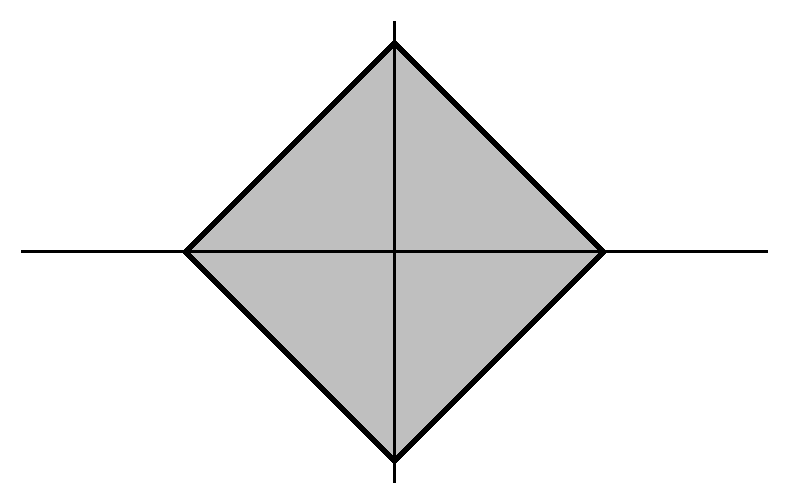
\includegraphics[width=0.15\textwidth]{norm1}\\
\norm{x}_2 & = \displaystyle\left(\sum_{i=1}^n\abs{x_i}^2\right)^{\frac{1}{2}} = \sqrt{x^*x}, & 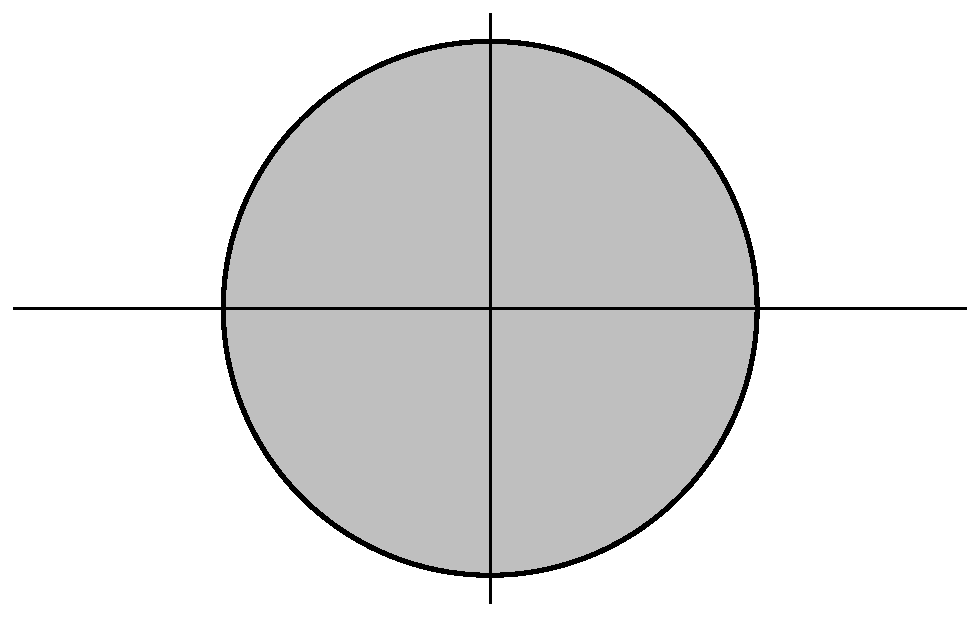
\includegraphics[width=0.15\textwidth]{norm2}\\
\norm{x}_p & = \displaystyle\left(\sum_{i=1}^n\abs{x_i}^p\right)^{\frac{1}{p}},\quad (1\le p < \infty), & 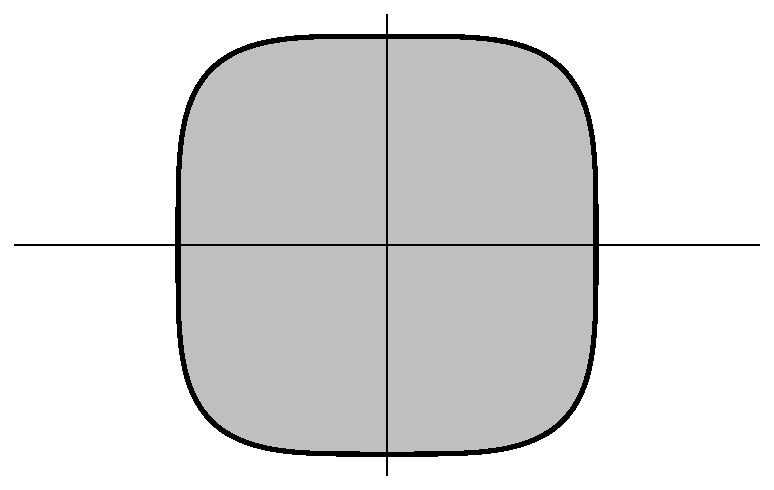
\includegraphics[width=0.15\textwidth]{norm4}\\
\norm{x}_\infty & = \displaystyle\max_{1\le i\le n}\abs{x_i}, & 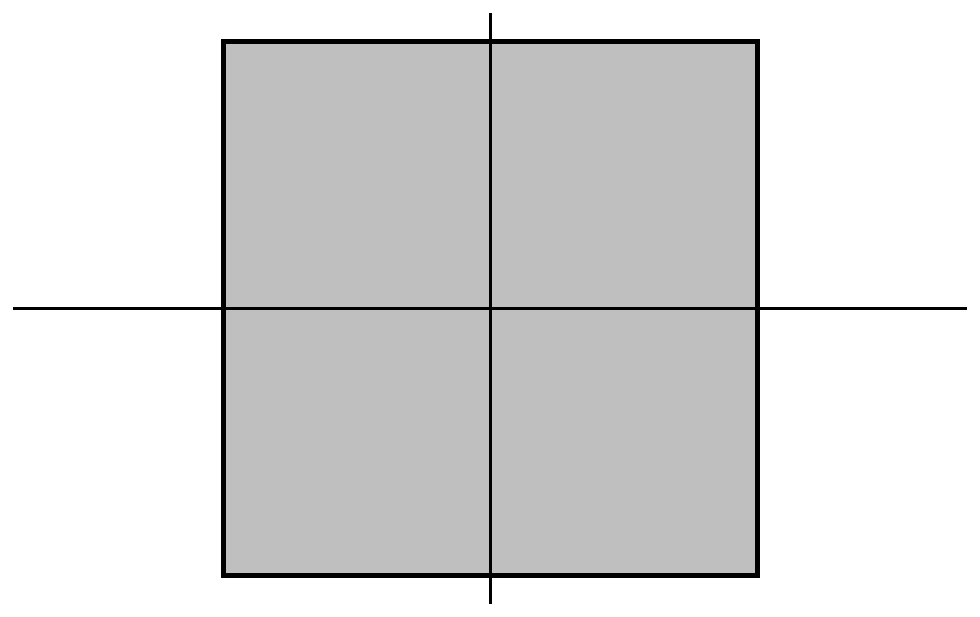
\includegraphics[width=0.15\textwidth]{norminf}\\
\end{array}
\end{equation}

The $2$-norm is the Euclidean length function; its unit ball is spherical. The $1$-norm is known as the Manhattan norm since it is the distance a taxi has to drive in a street grid\footnote{The $1$-norm is also used by airlines to define the maximal allowable size of a suitcase.}. The Sergel plaza in Stockhom, Sweden has the shape of the unit ball in the $4$-norm; the Danish poet Piet Hein popularized this ``superellipse'' as a pleasing shape for objects such as conference tables.

Aside from the $p$-norms, the most useful norms are the {\em weighted $p$-norms}, where each of the coordinates of a vector space is given its own weight. In general, given any norm $\norm{\cdot}$, a weighted norm can be written as:
\begin{equation}
\norm{x}_W = \norm{Wx}.
\end{equation}
Here, $W$ is the diagonal matrix in which the $i^{\rm th}$ diagonal entry is the weight $w_i\ne0$. For example, a weighted $2$-norm $\|\cdot\|_W$ on $\C^n$ is specified as follows:
\begin{equation}
\norm{x}_W = \left(\sum_{i=1}^n\abs{w_ix_i}^2\right)^{\frac{1}{2}}.\hspace*{2.5cm} 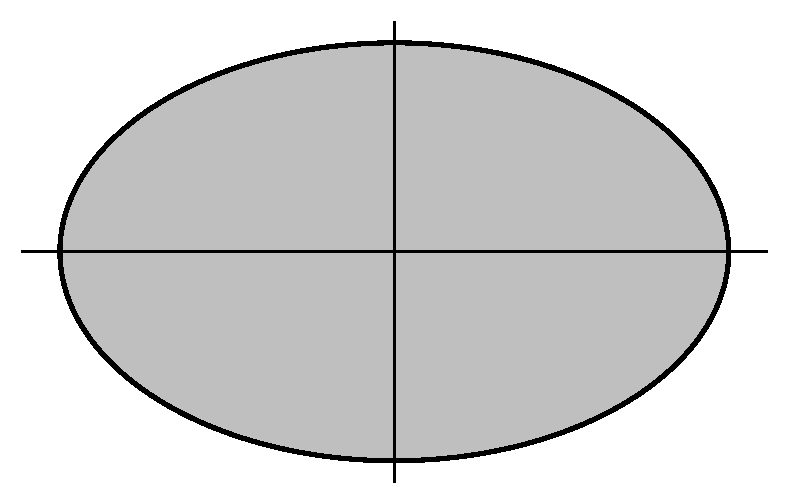
\includegraphics[width=0.15\textwidth]{normW}
\end{equation}
One can also generalize the idea of weighted norms by allowing $W$ to be an arbitrary nonsingular matrix.

The most important norms in this book are the unweighted $2$-norm and its induced matrix norm.

The concept of the $p$-norms can be extended to the case of vector spaces containing infinitely many elements. Such spaces are called sequence spaces, and the following spaces describe sequence spaces that have finite norm.

\begin{definition}
Let $1\le p\le\infty$. The space $\ell^p$ contains the set of all vectors $x\in V$ with finite $p$-norm:
\begin{equation}
\ell^p = \{ x\in V: \norm{x}_p < \infty\}.
\end{equation}
\end{definition}

\begin{example}
Every vector $x\in\R^n$ is in $\ell^p$. Consider the vector $y\in\R^\infty$ whose entries are defined by:
\begin{equation}
y_i = \dfrac{1}{i},\quad{\rm for}\quad i=1,\ldots,\infty.
\end{equation}
Then, $y\in\ell^p$ for every $p>1$ since for every $\epsilon>0$, $\sum_{i=1}^\infty i^{-1-\epsilon} < \infty$ by the integral test for convergence.
\end{example}

While we will not focus on $\ell^p$ spaces in this course, we will be interested in their analogues for functions.

\subsection{Function Spaces}

Let $D\subset\R$ or $\C$ denote the domain of a function $f$. 

\begin{definition}
A function is continuous at every point $c\in D$ if $f(c)$ exists and if $\displaystyle\lim_{\substack{x\to c \\ x \in D}}f(x) = f(c)$. \end{definition}

\begin{definition} The space:
\begin{itemize}
\item $C(D)$ contains all continuous functions on $D$;
\item $C^n(D)$ contains all functions whose $n^{\rm th}$ derivatives are continuous on $D$;
\item $C^\infty(D)$ contains all functions with continuous derivatives of all orders on $D$; and,
\item $A(D)$ contains all functions analytic on $D$. That is, they are equal to their Taylor series at every point in $D$.
\end{itemize}
\end{definition}

\begin{example}
The functions:
\begin{itemize}
\item $f(x) = \abs{x} \in C(\I)$;
\item $f(x) = \abs{x}^{n+1}\in C^n(\I)$ ($n$ even\footnote{For $n$ odd $\abs{x}^{n+1}$ is a polynomial and polynomials are entire.});
\item $f(x) = \left\{\begin{array}{ccc} e^{-1/x^2} & \for & x\ne 0,\\0 & \for & x = 0,\end{array}\right.\in C^\infty(D)$ for every $0\in D\subset\C$;
\item $f(x) = \dfrac{1}{1+x^2} \in A(D)$ where $D = \{z\in\C:\abs{z}<1\}$ is the open unit disk; and,
\item $f(x) = \sin x\in A(\C)$.
\end{itemize}
\end{example}

The analytic functions $A(\C)$ are so smooth that they are further denoted as {\em entire} functions.

The notion of a vector $p$-norm extends readily to functions that are Lebesgue integrable. For $1\le p < \infty$:
\begin{equation}
\|f\|_p := \left(\int_D\abs{f(x)}^p\ud x\right)^{\frac{1}{p}},
\end{equation}
and for $p=\infty$:
\begin{equation}
\|f\|_\infty := \sup_{x\in D} \abs{f(x)}.
\end{equation}
Sometimes the measure is not uniform. These cases correspond to the weighted $p$-norms:
\begin{equation}
\|f\|_{p,\mu} := \left(\int_D\abs{f(x)}^p\ud\mu(x)\right)^{\frac{1}{p}}.
\end{equation}

\begin{definition}
The space $L^p(D,\ud\mu(x))$ contains all functions Lebesgue\footnote{This definition ignores functions that are zero almost-everywhere, in which case the functions are indistinguishable from zero in norm since $\norm{f}_p=0$.} integrable on $D$ with respect to the measure $\ud\mu(x)$:
\begin{equation}
L^p(D,\ud\mu(x)) := \left\{ f : \norm{f}_{p,\mu} < \infty \right\}.
\end{equation}
\end{definition}

\begin{remark}
\begin{enumerate}
\item When it is clear from the context, the measure $\ud\mu(x)$ will dropped from the weighted $p$-norm;
\item The space $L^p(D) = L^p(D,\ud x)$; and,
\item If the measure $\mu \in C^1(D)$, then the space $L^p(D,{\rm\,d}\mu(x)) = L^p(D,w(x){\rm\,d}x)$ where $w(x) = \mu'(x)$.
\end{enumerate}
\end{remark}

\subsection{Inner Product Spaces}

Inner product spaces are vector spaces with an additional structure called an inner product.
\begin{definition}
An inner product $\langle\cdot,\cdot\rangle: V\times V\to\F$ is a sesquilinear map that assigns a value in the field $\F$ to two vectors in $V$. For all vectors $x,y,z\in V$ and for all scalars $\alpha,\beta\in\F$, the inner product satisfies:
\begin{enumerate}
\item conjugate symmetry: $\langle y,x\rangle = \conj{\langle x,y\rangle}$;
\item linearity in the second argument: $\langle x, \alpha y+\beta z\rangle = \alpha\langle x,y\rangle + \beta\langle x,z\rangle$; and,
\item positive-definiteness: $\langle x,x\rangle \ge 0$, and $\langle x,x\rangle = 0$ only if $x = 0$.
\end{enumerate}
\end{definition}

\begin{example}
For the vector spaces:
\begin{enumerate}
\item $V = \R^n$, we can define the inner product by the conventional dot product:
\[
\langle x,y \rangle := x^\top y = \sum_{i=1}^n x_iy_i;
\]
\item $V = \C^n$, we can define the inner product similarly:
\[
\langle x,y \rangle := x^* y = \sum_{i=1}^n x_i^*y_i;\quad and,
\]
\item $V = L^2(D,\ud\mu(x))$, we can define the inner product as:
\[
\langle f,g\rangle := \int_D\conj{f(x)}g(x)\ud\mu(x).
\]
\end{enumerate}
\end{example}
The inner products for $V = \R^n$ and $\C^n$ can be extended to the case where $n=\infty$.

\begin{example} For the normed vector spaces:
\begin{enumerate}
\item $V = \ell^2$, the norm can be defined in terms of the inner product:
\[
\norm{x}_2 := \sqrt{\langle x,x\rangle};\quad and,
\]
\item $V = L^2(D,\ud\mu(x))$, the norm can be defined similarly:
\[
\norm{f}_2 := \sqrt{\langle f,f\rangle}.
\]
\end{enumerate}
\end{example}

We can see that of the normed vector spaces described so far, $\ell^p$ spaces are generally {\em not} inner product spaces, and neither are the function spaces $L^p(D,\ud\mu(x))$. It is only when $p=2$ that we get normed inner product spaces.

The following inequality, known as the Cauchy--Schwarz inequality, is a useful inequality we will require further on.
\begin{theorem}
Let $u,v$ be arbitrary elements in an inner product space. Then, the following inequality holds:
\begin{equation}
\abs{\langle u,v\rangle} \le \norm{u}_2\norm{v}_2.
\end{equation}
\end{theorem}
\begin{proof}
If $\langle u,v\rangle =0$, the inequality is trivially true. Assume $u\ne 0$ and $v\ne 0$. If $\lambda = \dfrac{\overline{\langle u,v\rangle}}{\norm{v}_2^2}$, then:
\begin{align*}
0 \le \norm{u-\lambda v}_2^2 & = \langle u-\lambda v,u-\lambda v\rangle\\
& = \norm{u}_2^2 -\conj{\lambda}\langle v,u\rangle - \lambda\langle u,v\rangle +\lambda\conj{\lambda}\norm{v}_2^2,\\
& = \norm{u}_2^2 -\dfrac{\abs{\langle u,v\rangle}^2}{\norm{v}_2^2} - \dfrac{\abs{\langle u,v\rangle}^2}{\norm{v}_2^2} +\dfrac{\abs{\langle u,v\rangle}^2}{\norm{v}_2^2},\\
& = \norm{u}_2^2 -\dfrac{\abs{\langle u,v\rangle}^2}{\norm{v}_2^2},
\end{align*}
and the inequality follows by rearranging terms.
\end{proof}

\begin{example}
For the inner product spaces:
\begin{enumerate}
\item $V=\ell^2$, the Cauchy--Schwarz inequality reads:
\[
\abs{\sum_{i=1}^n \conj{x_i}y_i}^2 \le \left(\sum_{i=1}^n\abs{x_i}^2\right)\left(\sum_{i=1}^n\abs{y_i}^2\right);\quad and,
\]
\item $V=L^2(D,\ud\mu(x))$, the Cauchy--Schwarz inequality reads:
\[
\abs{\int_D\conj{f(x)}g(x)\ud\mu(x)}^2 \le \int_D\abs{f(x)}^2\ud\mu(x)\int_D\abs{g(x)}^2\ud\mu(x).
\]
\end{enumerate}
\end{example}

\subsection{Matrix Norms Induced by Vector Norms}

An $m\times n$ matrix can be viewed as a vector in an $mn$-dimensional space: each of the $mn$ entries of the matrix is an independent coordinate. Any $mn$-dimensional norm can therefore be used for measuring the ``size'' of such a matrix.

However, in dealing with a space of matrices, certain special norms are more useful than the vector norms already discussed. These are the {\em induced matrix norms}, defined in terms of the behaviour of a matrix as an operator between its normed domain and range spaces.

Given a vector $p$-norm $\norm{\cdot}_p$, the induced matrix norm $\norm{A}_p$ is the smallest number $C$ for which the following inequality holds for all $x\in\C^n$:
\begin{equation}
\norm{Ax}_p \le C\norm{x}_p.
\end{equation}
In other words, $\norm{A}_p$ is the supremum of the ratios $\norm{Ax}_p/\norm{x}_p$ over all vectors $x\in\C^n$--the maximum factor by which $A$ can ``stretch'' a vector $x$. We say that $\norm{\cdot}_p$ is the matrix norm induced by $\norm{\cdot}_p$.

Because of condition 3.~of Definition~\ref{definition:norm} the action of $A$ is determined by its action on unit vectors. Therefore, the matrix norm can be defined equivalently in terms of the images of the unit vectors under $A$:
\begin{equation}
\norm{A}_p = \sup_{\substack{x\in\C^n\\x\ne0}}\dfrac{\norm{Ax}_p}{\norm{x}_p} = \max_{\substack{x\in\C^n\\ \norm{x}_p = 1}}\norm{Ax}_p.
\end{equation}
This form of the definition can be convenient for visualizing induced matrix norms.

\begin{example}
The matrix:
\begin{equation}
A = \begin{bmatrix}
1 & 2\\ 0 & 2\\
\end{bmatrix},
\end{equation}
maps $\C^2$ to $\C^2$. It also maps $\R^2$ to $\R^2$, which is more convenient if we want to draw pictures and also (it can be shown) sufficient for determining matrix $p$-norms, since the coefficients of $A$ are real.

Figure~\ref{figure:InducedNorms} depicts the action of $A$ on the unit balls of $\R^2$ defined by the $1$-, $2$-, and $\infty$-norms. From this figure, one can see a graphical interpretation of these three norms of $A$. Regardless of the norm, $A$ maps $e_1 = (1,0)^\top$ to the first column of $A$, namely $e_1$ itself, and $e_1=(0,1)^\top$ to the second column of $A$, namely, $(2,2)^\top$. In the $1$-norm, the unit vector $x$ that is amplified most by $A$ is $(0,1)^\top$ (or its negative), and the amplification factor is $4$. In the $\infty$-norm, the unit vector $x$ that is amplified most by $A$ is $(1,1)^\top$ (or its negative), and the amplification factor is $3$. In the $2$-norm, the unit vector that is amplified most by $A$ is the vector indicated by the dashed line in the figure (or its negative), and the amplification factor is approximately $2.9208$. (Note that it must be at least $\sqrt{8}\approx 2.8284$, since $(0,1)^\top$ maps to $(2,2)^\top$.) We shall consider how to calculate such $2$-norm results in Chapter~\ref{chapter:LinearSystems}.

\begin{figure}[htbp]
\begin{center}
{\renewcommand{\tabularxcolumn}[1]{m{#1}}
\begin{tabularx}{\textwidth}{XXXXX}
$1$-norm: &
\hspace*{-1.5cm}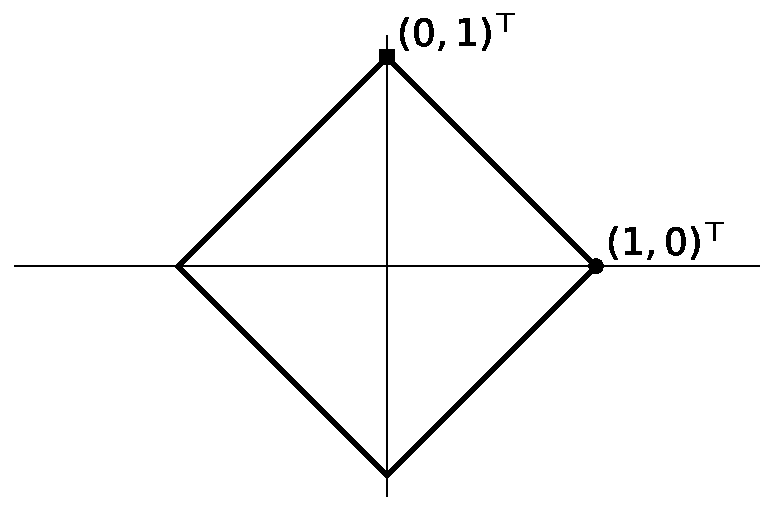
\includegraphics[width=0.25\textwidth]{norm1annotated}&
$\rightarrow$&
\hspace*{-2cm}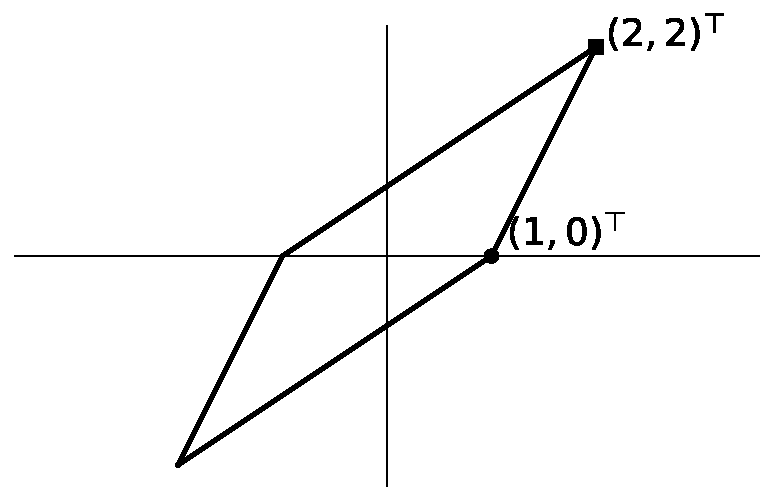
\includegraphics[width=0.25\textwidth]{normA1annotated}&
$\norm{A}_1=4$\\
$2$-norm: &
\hspace*{-1.5cm}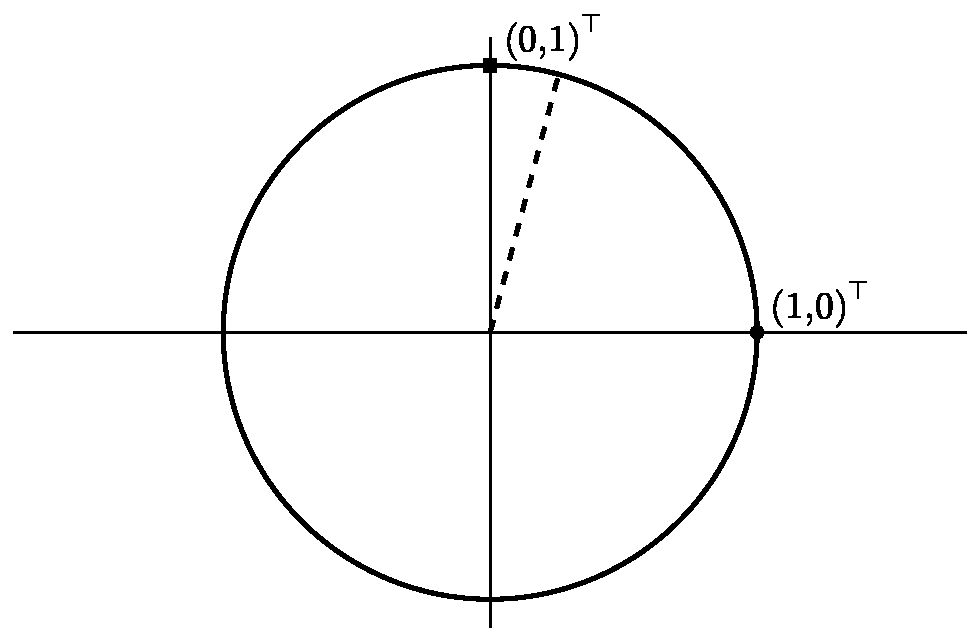
\includegraphics[width=0.25\textwidth]{norm2annotated}&
$\rightarrow$&
\hspace*{-2cm}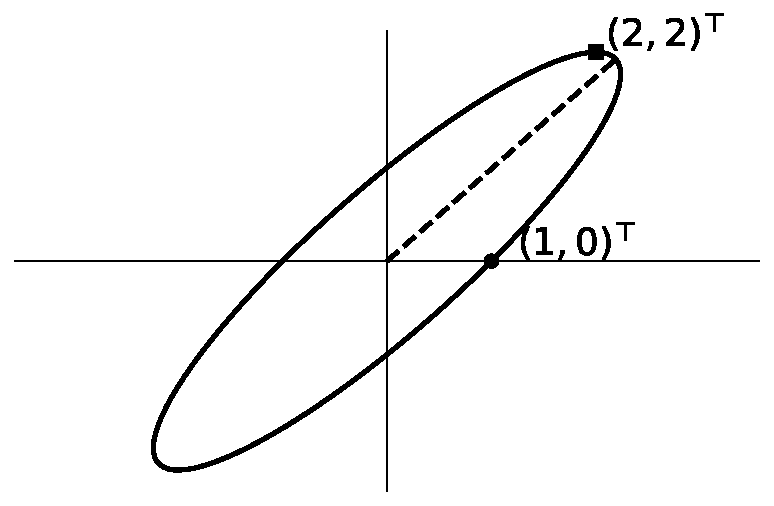
\includegraphics[width=0.25\textwidth]{normA2annotated}&
$\norm{A}_2\approx 2.9208$\\
$\infty$-norm: &
\hspace*{-1.5cm}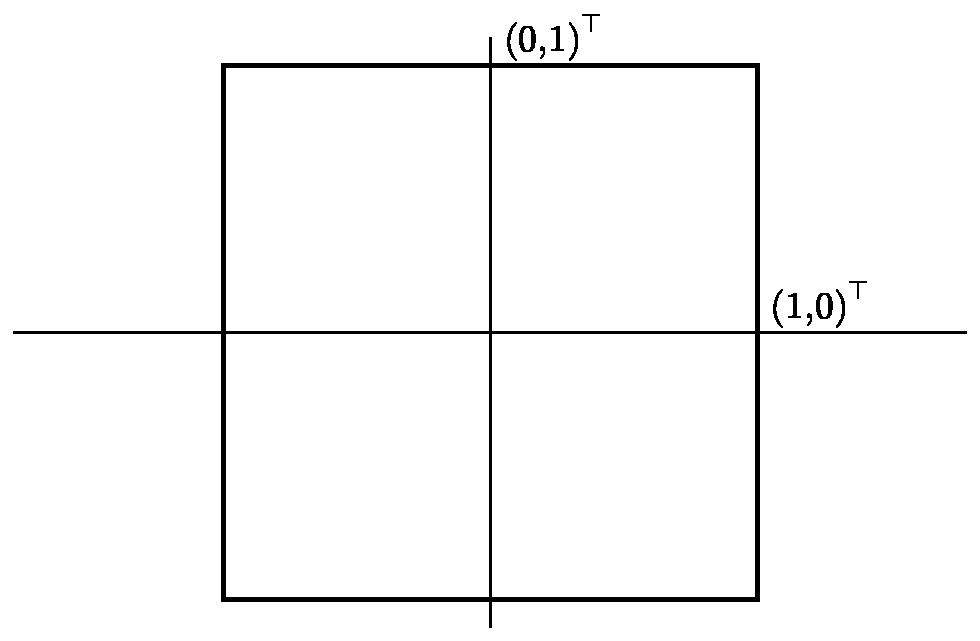
\includegraphics[width=0.25\textwidth]{norminfannotated}&
$\rightarrow$&
\hspace*{-2cm}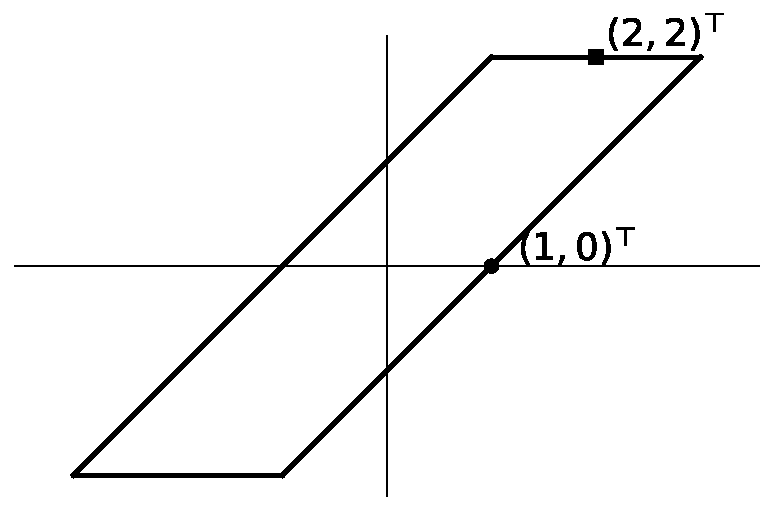
\includegraphics[width=0.25\textwidth]{normAinfannotated}&
$\norm{A}_\infty=3$\\
\end{tabularx}}
\caption{The induced matrix $1$-, $2$-, and $\infty$-norms of $A$.}
\label{figure:InducedNorms}
\end{center}
\end{figure}
\end{example}

\begin{example}\label{example:diagonalpnorm}
The $p$-norm of a diagonal matrix. Let $D$ be the diagonal matrix:
\begin{equation}
D = \begin{bmatrix} d_1\\ &d_2\\&&\ddots\\&&&d_n\end{bmatrix}.
\end{equation}
Then, as in the second row of Figure~\ref{figure:InducedNorms}, the image of the $2$-norm unit sphere under $D$ is an $n$-dimensional ellipse whose semiaxis lengths are given by the numbers $\abs{d_i}$. The unit vectors amplified most by $D$ are those that are mapped to the longest semiaxis of the ellipse, of length $\max_i\{\abs{d_i}\}$. Therefore, we have $\displaystyle \norm{D}_2 = \max_{1\le i\le n}\{\abs{d_i}\}$.

This result for the $2$-norm generalizes to any $p$: if $D$ is diagonal, then $\displaystyle \norm{D}_p = \max_{1\le i\le n}\{\abs{d_i}\}$.
\end{example}

\begin{example}
The $1$-norm of a matrix. If $A$ is any $m\times n$ matrix, then $\norm{A}_1$ is equal to the ``maximum column sum'' of $A$. We explain and derive this result as follows. Write $A$ in terms of its columns:
\begin{equation}
A = \begin{bmatrix} a_1 & \Bigg| & \cdots & \Bigg| & a_n\end{bmatrix},
\end{equation}
where each $a_j$ is an $m$-vector. Consider the diamond-shaped $1$-norm unit ball in $\C^n$, illustrated in Figure~\ref{figure:InducedNorms}. This is the set $\{x\in\C^n:\sum_{j=1}^n\abs{x_j} \le 1\}$. Any vector $Ax$ in the image of this set satisfies:
\begin{equation}
\norm{Ax}_1 = \norm{\sum_{j=1}^nx_ja_j}_1 \le \sum_{j=1}^n\abs{x_j}\norm{a_j}_1 \le \max_{1\le j\le n}\norm{a_j}_1.
\end{equation}
Therefore, the induced matrix $1$-norm satisfies $\norm{A}_1 \le \max_{1\le j\le n}\norm{a_j}_1$. By choosing $x=e_j$, where $j$ maximizes $\norm{a_j}_1$, we attain this bound, and thus the matrix norm is:
\begin{equation}
\norm{A}_1 = \max_{1\le j\le n}\norm{a_j}_1.
\end{equation}
\end{example}

\begin{example}
The $\infty$-norm of a matrix. By much the same argument, it can be shown that the $\infty$-norm of an $m\times n$ matrix is equal to the ``maximum row sum:''
\begin{equation}
\norm{A}_\infty = \max_{1\le i\le m}\norm{a_i^*}_1,
\end{equation}
where $a_i^*$ denotes the $i^{\rm th}$ row of $A$.
\end{example}

Finally, it should be clear that induced norms are submultiplicative, since:
\[
\norm{AB}_p = \sup_{\substack{x\in\C^n\\x\ne0}}\dfrac{\norm{ABx}_p}{\norm{x}_p} = \sup_{\substack{x\in\C^n\\x\ne0\\Bx\ne0}}\dfrac{\norm{ABx}_p}{\norm{Bx}_p}\dfrac{\norm{Bx}_p}{\norm{x}_p} \le \sup_{\substack{y\in\C^n\\y\ne0}}\dfrac{\norm{Ay}_p}{\norm{y}_p}\sup_{\substack{x\in\C^n\\x\ne0}}\dfrac{\norm{Bx}_p}{\norm{x}_p} = \norm{A}_p\norm{B}_p.
\]

\section{Computer Representation of Numbers}

Bits are the smallest piece of information that can be stored in memory on a digital computer. Their role is similar to the role played by atomic particles in quantum physics. The simplest type of numbers we can store with one bit are the Boolean numbers \verb+true+ and \verb+false+. If bits can take on at least two distinct values, such as yes/no or on/off, then Boolean numbers can be represented in one bit.

\subsection{Integers}

The most important integers we can represent on a digital computer are those nearest to $0$. Let $b\in\N$ be a {\em radix}, which is Latin for root or base. Integers can be represented in radix-$b$ as:
\[
\pm(d_kd_{k-1}\cdots d_0)_b = \pm\left(d_kb^k + d_{k-1}b^{k-1} + \cdots + d_0\right),
\]
where the numbers $0\le d_k < b$. In this representation, integers from $0$ to:
\[
(b-1)(b^k+b^{k-1}+\cdots+1) = b^{k+1}-1,
\]
each have a unique signature, and similarly for negative integers from\footnote{We can represent one more negative integer because we only need one $0$.} $-b^{k+1}$ up to $-1$. Using a finite number of bits, a finite number of integers can be represented on a digital computer. As the sign bit behaves just as a Boolean number, we need one extra bit for its inclusion.

\subsection{Fixed-Point Numbers}

Fixed-point numbers are approximations to real numbers $\R$ with a fixed number of digits before the radix point `.' and another fixed number of digits after the radix point:
\[
\pm(d_kd_{k-1}\cdots d_0.d_{-1}\cdots d_{-n})_b = \pm\left(d_kb^k + d_{k-1}b^{k-1} + \cdots + d_0 + d_{-1}b^{-1} + \cdots + d_{-n}b^{-n}\right).
\]
Because fixed-point operations can easily produce results that require more bits than the operands\footnote{If $c = a+b$, then $+$ is the operator and $a$ and $b$ are operands.}, there is possibility for information loss. In scientific computing, fixed-point numbers have fallen from favour because of the need to have scale-invariance in calculations: consider performing any calculation with Planck's constant $h \approx 6.63\times10^{-34}{\rm\,J}\cdot{\rm s}$ and the speed of light squared $c^2 \approx 8.99\times10^{16}{\rm\,m}^2/{\rm s}^2$. This would be an expensive calculation in fixed-point arithmetic, yet it could more easily be done by hand.

\subsection{Floating-Point Numbers}

Modern computers are all binary\footnote{In the 1950's, the Soviets experimented with a balanced ternary (or trinary) computer called Setun, whose bits took the values $\{-1,0,1\}$. The mass production of binary computers has diminished the importance of ternary computing, though it may make a comeback with optical computing.}, whose binary bits can take the value $0$ or $1$. Groups of eight contiguous bits make up a byte; $2^{10}$ bytes make a kilobyte (KB); $2^{20}$ bytes make a megabyte (MB); $2^{30}$ bytes make a gigabyte (GB) and so on and so forth.

The IEEE Standard for Floating-Point Arithmetic (IEEE 754) includes a directive on how to create floating-point numbers to approximate the real numbers on a computer. (Normalized) floating-point numbers are alternative approximations to the reals $\R$ with a fixed number of digits after the radix point {\em multiplied by} a power $p-M$ of the base $2$:
\[
\pm 2^{p-M} \times (1.d_{-1}\cdots d_{-n})_2  = \pm\left(2^{p-M} + d_{-1}2^{p-M-1} + \cdots + d_{-n}2^{p-M-n}\right).
\]
As with the integers and fixed-point numbers, one bit is used to store the sign of the floating-point number, $n$ bits are used for the fractional part known as the {\em mantissa}, and the {\em exponent} $p$ is represented by an unsigned integer. If we use $m$ bits to represent $p$, then we can choose to use the $2^m$ integers in the range $0 \le p < 2^m$. In total, then, we require $1+m+n$ bits to represent the floating-point number. $M$ is known as the {\em exponent bias}.

The IEEE 754 standard prescribes Table~\ref{table:IEEEFloatingPoint} for binary floating-point numbers.

\begin{table}[htdp]
\caption{IEEE 754 standard for binary signed floating-point representation of numbers.}
\begin{center}
\begin{tabular}{ccccccccc}
\hline
Common Name & Base & Digits & Decimal Digits & E Bits & E min & E max & Decimal E max & $M$\\
\hline
Half precision  & $2$ & $10$ & $3.01$ & $5$ & $-14$ & $+15$ & $4.51$ & $15$\\
Single precision  & $2$ & $23$ & $6.92$ & $8$ & $-126$ & $+127$ & $38.23$ & $127$\\
Double precision  & $2$ & $52$ & $15.65$ & $11$ & $-1022$ & $+1023$ & $307.95$ & $1023$\\
\hline
\end{tabular}
\end{center}
\label{table:IEEEFloatingPoint}
\end{table}%

Notice in Table~\ref{table:IEEEFloatingPoint} that the exponent minimum and maximum values fall just short of the maximum allowable range given the number of bits. Subnormal numbers, that is, numbers below $2^{-1022}$ in double precision for example, can only be represented with fewer digits because some of these digits take the surrogate role of extending the power of the exponent.\footnote{Furthermore, subnormal numbers are denormalized and thus start with a $0$ rather than a $1$.} Indeed, the smallest representable number in double precision is $2^{-1022-52} = 2^{-1074}$.

\begin{example}
\begin{itemize}
\item Numbers in double precision, with exponent bias $M=1023$, are stored as:

$\underbrace{\red a}_{\rm 1~sign~bit}\underbrace{\green bbbbbbbbbbb}_{\rm 11~exponent~bits}\underbrace{\blue cccccccccccccccccccccccccccccccccccccccccccccccccccc}_{\rm 52~significand~bits}$

\item For example, $1.0$ is represented by:

{\red0}{\green01111111111}{\blue0000000000000000000000000000000000000000000000000000}

\item and $-29.0$ is:

{\red1}{\green10000000011}{\blue1101000000000000000000000000000000000000000000000000}
\end{itemize}
\end{example}

Floating-point numbers are more versatile than fixed-point numbers because they are distributed in a way which preserves an approximately constant relative precision throughout the range of values they can represent: the density of floating-point numbers accumulates near $0$ and disperses at infinity. In double precision, floating-point numbers are equally distributed in $[\tfrac{1}{2},1)$ with spacing $2^{-53}$, equally distributed in $[1,2)$ with spacing $2^{-52}$, equally distributed in $[2,4)$ with spacing $2^{-51}$ and so on and so forth, and equally distributed in $[\tfrac{1}{4},\tfrac{1}{2})$ with spacing $2^{-54}$, and so on and so forth, as illustrated below.
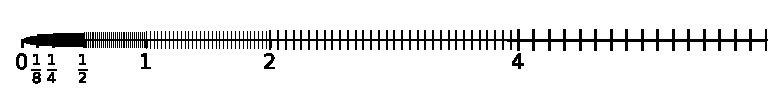
\includegraphics[width=\textwidth]{FloatingPoint}

\subsubsection{How continuous is real life?}

Having decided to approximate real numbers by floating-point numbers on a computer, we might ask how accurately we can represent real life. Avogadro's number $N_A \approx 6.02\times10^{23}{\rm\,molecules}/{\rm mol}$ tells us how many molecules of anything are in one mol. Now, for the sake of the argument, let us take $1{\rm\,m}^3$ of the air with density $\rho = 1.225{\rm\,kg}/{\rm m}^3$ in between you and me. In this cubic meter of air, consisting of roughly $78\%$ nitrogen with a molar mass of $M(N_2) = 28.02{\rm\,g}/{\rm mol}$, we find that there are:
\[
N_A \times M(N_2)^{-1} \times \dfrac{1000{\rm\,g}}{1{\rm\,kg}} \times \rho \times 1{\rm\,m}^3 \approx 2.63\times10^{25}{\rm\,molecules},
\]
of nitrogen in this cubic meter of air. If we assume they are uniformly distributed, then there are only:
\[
\sqrt[3]{2.63\times10^{25}}{\rm\,molecules} \approx 3\times10^8{\rm\,molecules},
\]
lined up in $1{\rm~m}$ in any given direction.

On the other hand, with IEEE double precision floating-point numbers we can distinguish numbers at the scale of one unit of least precision (ulp), that is, the value the least significant digit represents if it is $1$, which is $\approx2.2045\times10^{-16}$ in double precision. Therefore, while we sometimes think of real life as continuous and digital computation as discrete, it is now the case that the level of discreteness on today's computers can be regarded as more refined than real life!

\subsection{The Standard Model}

To store a real number, that is, to obtain a machine representation of a real number, we must truncate the fractional part of the binary expansion of the real number to $n$ bits, the number of bits in the mantissa. This is done by truncating (ignoring all digits after the $n^{\rm th}$ bit) or by rounding. In the latter, if the $(n+1)^{\rm th}$ bit of the expansion of the given number is one, then we round up (taking the first $n$ bits and adding one to the last bit). Otherwise, we simply take the first $n$ bits as in truncation.

Floating-point arithmetic does not obey the usual rules of arithmetic such as the laws of associativity and distributivity. When programming, it is better practice to avoid statements such as:
\begin{verbatim}
if x == .3 then...
\end{verbatim}
Here, rounding errors may mean that the conditional code block is not executed even if the mathematical value of $x$ is $.3$. In this case, it is better to test \verb+if |x-.3| < tol+ where \verb+tol+ is some small tolerance.

For a real number $x$, we denote floating-point approximations to quantities by $\fl(x)$. Using Higham's standard model for floating-point arithmetic~\cite{Higham-02}, we assume that whenever $x$ and $y$ are floating-point numbers and $\circledast$ is one of the four arithmetic operations $+$, $-$, $\times$, or $\div$, we have:
\begin{equation}
\fl(x\circledast y) = (x\circledast y)(1+\delta)^{\pm1},\quad{\rm where}\quad |\delta| \le \epsilon,
\end{equation}
where $\epsilon$ is a unit of least precision.

\begin{lemma}[Higham~\cite{Higham-02}]
If $|\delta_i|\le \epsilon$, and $\rho_i=\pm1$ for $i=1,\ldots,n$, and $n\epsilon<1$, then:
\begin{equation}
\langle n \rangle := \prod_{i=1}^n(1+\delta_i)^{\rho_i} = 1+\theta_n,\qquad |\theta_n| \le \dfrac{n\epsilon}{1-n\epsilon} =:\gamma_n.
\end{equation}
\end{lemma}
\begin{proof}
The proof is by induction.
\end{proof}
The notation $\langle n \rangle$ is useful as a counter to show the accumulation of $n$ relative errors due to rounding. The counters can be manipulated using the rules:
\begin{align}
\langle m\rangle + \langle n\rangle & = \langle\max\{m,n\}\rangle,\\
\langle m\rangle - \langle n\rangle & = \langle\max\{m,n\}\rangle,\\
\langle m\rangle\langle n\rangle & = \langle m+n\rangle,\\
\dfrac{\langle m\rangle}{\langle n\rangle} & = \langle m+n\rangle.
\end{align}

\subsection{Cancellation Error}

Cancellation error is the loss of significant digits when subtracting two nearly equal floating-point numbers. In base-$10$ and with $6$ digits, suppose we wish to find the difference of $1.2345671$ and $1.2345660$. After rounding:
\[
\fl(1.234567-1.234566) = 0.000001 = 1.000000\times10^{-6},
\]
a result which has only one correct digit. This phenomenon can lead to an answer which is completely different from the exact one, especially over the course of a long sequence of operations.

\begin{example}
In base-$10$ and with three digits:
\[
\fl(\fl(\sqrt{9.01})-3.00) = \fl(3.00-3.00) = 0,
\]
which is very different from the exact answer $\approx 1.6662\times10^{-3}$. 

Observe that:
\[
\sqrt{9.01}-3 = (\sqrt{9.01}-3)\dfrac{\sqrt{9.01}+3}{\sqrt{9.01}+3} = \dfrac{0.01}{\sqrt{9.01}+3}.
\]
Calculation of this quantity using the last expression has no cancellation error and leads to $1.67\times10^{-3}$ which is as good as one can expect with three digits.
\end{example}

\begin{example}
Solve $x^2+10^9x-3=0$. By the quadratic formula, the two roots are:
\[
x_- = \dfrac{-10^9-\sqrt{10^{18}+12}}{2},\qquad x_+ = \dfrac{-10^9+\sqrt{10^{18}+12}}{2}.
\]
There is no cancellation in $x_-$ which can be computed accurately in double precision. On the other hand, $x_+$ is a difference of nearly equal numbers. In double precision, the result is exactly zero. As above, a better calculation is:
\[
x_+ = \dfrac{-10^9+\sqrt{10^{18}+12}}{2}\dfrac{10^9+\sqrt{10^{18}+12}}{10^9+\sqrt{10^{18}+12}} = \dfrac{6}{10^9+\sqrt{10^{18}+12}},
\]
which is accurately computed in double precision.
\end{example}

\begin{example}
Consider evaluation of $f(x) = \dfrac{\log(1+x)}{x}$ in a neighbourhood of $x=0$. By l'H\^opital's rule, $f(0)=1$. The na\"ive way to evaluate $f$ suffers from serious cancellation error near $x=0$. In floating-point arithmetic, a better way is the following:
\[
\left\{ \begin{array}{ccc}
\dfrac{\log(\fl(1+x))}{\fl(\fl(1+x)-1)}, & \for & \fl(1+x)\ne 1,\\
1, & \for & \fl(1+x)=1.
\end{array}\right.
\]
Another alternative is to use the (standard) library function $\logop$, defined by its Taylor series near $x=1$ and by $\log\fl(1+x)$ sufficiently far away to cause no loss of accuracy, such that $f(x) = \logop(x)/x$. Figure~\ref{figure:log1pdx} shows the relative error in approximating $f$ using all three methods.
\begin{figure}[htbp]
\begin{center}
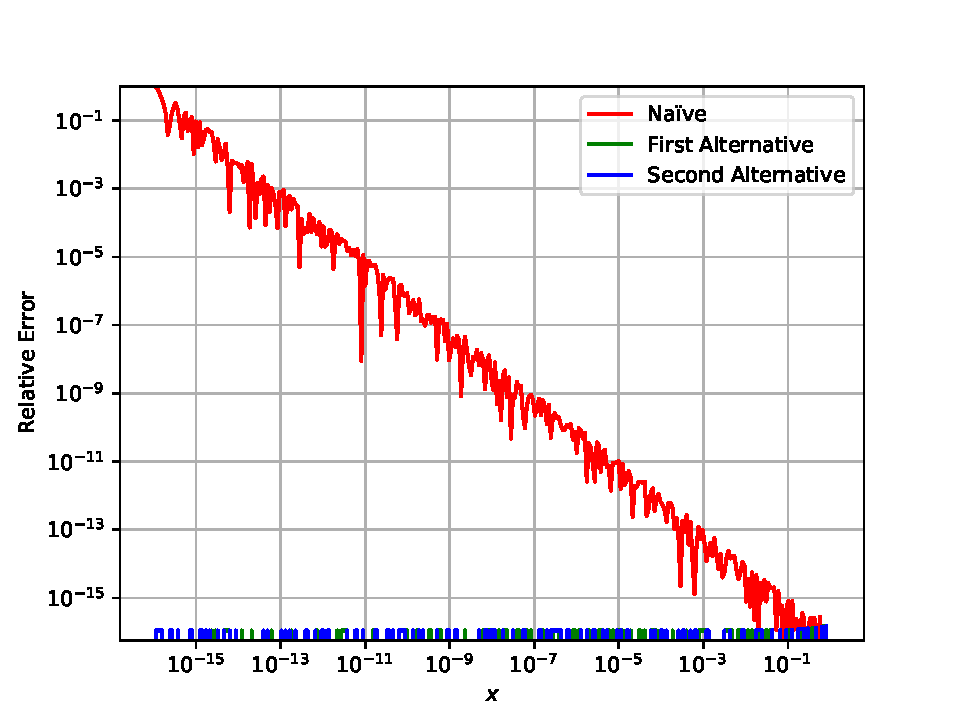
\includegraphics[width=0.65\textwidth]{log1pdx}
\caption{Comparison of the na\"ive and alternative methods for computing $f(x) = \frac{\log(1+x)}{x}$.}
\label{figure:log1pdx}
\end{center}
\end{figure}
\end{example}

Sums of floating-point numbers are ubiquitous in scientific computing. They occur when evaluating inner products, norms, means, variances, and all kinds of nonlinear functions. Although at first sight summation might appear to offer little scope for algorithmic ingenuity, the usual ``recursive summation'' (with various orderings) is just one of a variety of possible techniques. We describe several summation methods and their error analyses in the next example. No one method is uniformly more accurate than the others, but some guidelines can be given on the choice of method in particular cases.

\begin{example}
Consider the computation of $\displaystyle S_n = \sum_{i=1}^nx_i$ using the following algorithms:
\begin{enumerate}
\item Recursive summation, where we set $s=0$ and recursively add $x_i$ to $s$ for $i=1,\ldots,n$; and,
\item Pairwise summation (also know as cascade summation), where the $x_i$ are summed in pairs according to:
\[
y_i = x_{2i-1}+x_{2i},\quad{\rm for}\quad i=1,\ldots\lfloor\tfrac{n}{2}\rfloor,\quad (y_{(n+1)/2} = x_n\hbox{ if }n\hbox{ is odd}),
\]
and this pairwise summation repeats recursively on the $y_i$, obtaining the sum in $\lceil\log_2n\rceil$ stages.
\end{enumerate}
Using the standard model, recursive summation leads to the accumulation of $\langle n-1\rangle$ rounding errors, while pairwise summation only leads to the accumulation of $\langle \lceil\log_2 n\rceil\rangle$ rounding errors. For example, for recursive summation of $S_8$, we have:
\begin{align*}
\fl(S_8) & = \fl(\fl(\fl(\fl(\fl(\fl(\fl(x_1+x_2)+x_3)+x_4)+x_5)+x_6)+x_7)+x_8),\\
& = (((((((x_1+x_2)\langle1\rangle+x_3)\langle1\rangle+x_4)\langle1\rangle+x_5)\langle1\rangle+x_6)\langle1\rangle+x_7)\langle1\rangle+x_8)\langle1\rangle,\\
& = (((((((x_1+x_2)\langle2\rangle+x_3\langle1\rangle)+x_4)\langle1\rangle+x_5)\langle1\rangle+x_6)\langle1\rangle+x_7)\langle1\rangle+x_8)\langle1\rangle,\\
& = ((((((x_1+x_2+x_3)\langle2\rangle+x_4)\langle1\rangle+x_5)\langle1\rangle+x_6)\langle1\rangle+x_7)\langle1\rangle+x_8)\langle1\rangle,\\
& = (((((x_1+x_2+x_3+x_4)\langle3\rangle+x_5)\langle1\rangle+x_6)\langle1\rangle+x_7)\langle1\rangle+x_8)\langle1\rangle,\\
& = ((((x_1+x_2+x_3+x_4+x_5)\langle4\rangle+x_6)\langle1\rangle+x_7)\langle1\rangle+x_8)\langle1\rangle,\\
& = (((x_1+x_2+x_3+x_4+x_5+x_6)\langle5\rangle+x_7)\langle1\rangle+x_8)\langle1\rangle,\\
& = ((x_1+x_2+x_3+x_4+x_5+x_6+x_7)\langle6\rangle+x_8)\langle1\rangle,\\
& = S_8\langle7\rangle.
\end{align*}
On the other hand, for pairwise summation of $S_8$, we have:
\begin{align*}
\fl(S_8) & = \fl(\fl(\fl(x_1+x_2) + \fl(x_3+x_4)) + \fl(\fl(x_5+x_6) + \fl(x_7+x_8))),\\
& = (((x_1+x_2)\langle1\rangle + (x_3+x_4)\langle1\rangle)\langle1\rangle + ((x_5+x_6)\langle1\rangle + (x_7+x_8)\langle1\rangle)\langle1\rangle)\langle1\rangle,\\
& = ((x_1+x_2+x_3+x_4)\langle2\rangle + (x_5+x_6+x_7+x_8)\langle2\rangle)\langle1\rangle,\\
& = S_8\langle3\rangle.
\end{align*}
Note that there are even other alternative methods, and even changing the direction of the recursive summation can lead to an improvement in certain sums. For example, if the sequence $\abs{x_i}$ is decreasing, the reverse recursive summation can be even more accurate than pairwise summation, exhibiting no error growth with $n$! This shows that when we start making assumptions on $x_i$, the error analysis with counters can be made more precise. This also shows that no algorithm is uniformly more accurate. Figure~\ref{figure:summation} compares forward/reverse recursive and pairwise summation for a given sequence.
\begin{figure}[htbp]
\begin{center}
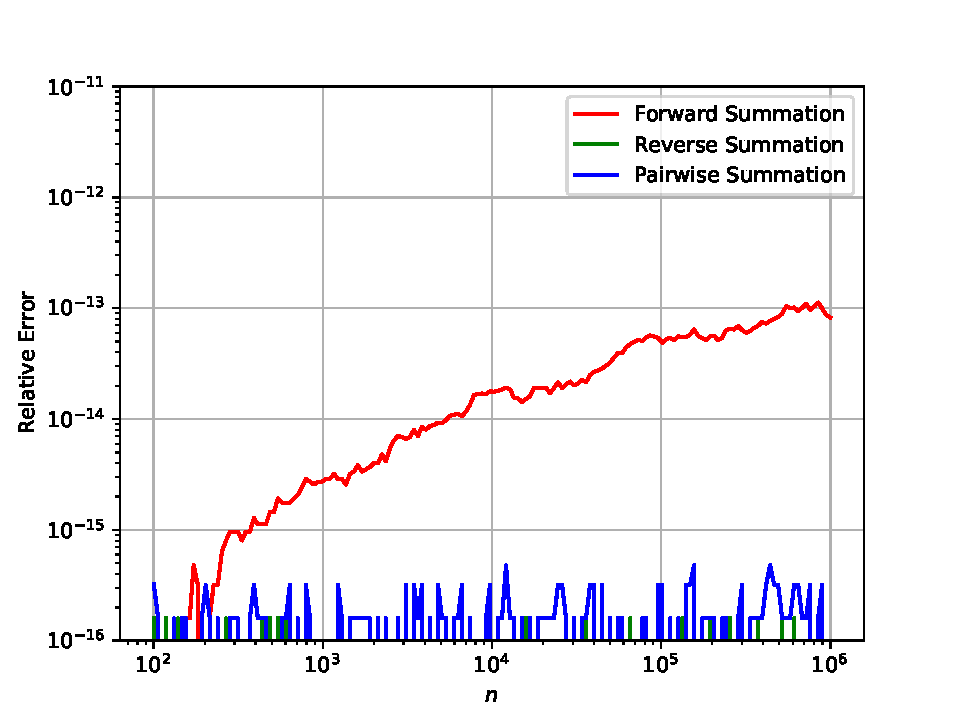
\includegraphics[width=0.65\textwidth]{summation}
\caption{Comparison of the recursive and pairwise summation algorithms for $\displaystyle S_n = \sum_{i=1}^n\dfrac{(-1)^i}{i}$.}
\label{figure:summation}
\end{center}
\end{figure}
\end{example}

\section{Conditioning and Stability}

A problem typically has an input and an output. The input consists of a set of data, say, the coefficients of some equation, and the output of another set of numbers uniquely determined by the input, say, all the roots of the equation in some prescribed order. If we collect the input in a vector $x\in X$, and the output in the vector $y\in Y$, where $X$ and $Y$ are normed vector spaces, we may thus think of a problem as a map $f$, given by:
\begin{equation}
f:X\to Y,\quad y = f(x).
\end{equation}
What we are interested in is the sensitivity of the map $f$ at some given point $x$ to a small perturbation of $x$, that is, how much bigger (or smaller) is the perturbation in $y$ compared to the perturbation in $x$? In particular, we wish to measure the degree of sensitivity by a single number -- the {\em condition number} of the map $f$ at the point $x$. We emphasize that, as we perturb $x$, the function $f$ is always assumed to be evaluated exactly, with infinite precision. The condition of $f$, therefore is an inherent property of the map $f$ and does not depend on any algorithmic considerations concerning its implementation in finite precision on a computer.

This is not to say that knowledge of the condition of a problem is irrelevant to any algorithmic solution of the problem. On the contrary, the reason is that quite often the {\em computed solution} $y^*$, using a specific algorithm in finite precision, can be demonstrated to be the {\em exact} solution to a ``nearby'' problem, that is:
\begin{equation}
y^* = f(x^*),
\end{equation}
where $x^*$ is a point close to the given data $x$:
\begin{equation}
x^* = x+\Delta x,
\end{equation}
and moreover, the distance $\norm{\Delta x}_X$ of $x^*$ to $x$ can be estimated in terms of the machine precision. Therefore, if we know how strongly (or weakly) the map $f$ reacts to a small perturbation, such as $\Delta x$, we can say something about the error $\norm{y^*-y}_Y$ in the solution caused by this perturbation. This, indeed, is an important technique of error analysis -- know as {\em backward error analysis} -- which was pioneered in the 1950's by Givens, Lanczos, and Wilkinson.

\begin{example}
\begin{enumerate}
\item For a given matrix $A\in\R^{m\times n}$, define the problem of matrix-vector multiplication $f:\R^n\to\R^m$ with the Euclidean norms on the input and output:
\begin{equation}
f(x) = Ax.
\end{equation}
This problem encodes the sensitivity of matrix-vector multiplication to perturbations in the {\em vector}.
\item For a given vector $x\in\R^n$, define the problem of matrix-vector multiplication $f:\R^{m\times n}\to\R^m$ with the (induced) $2$-norms on the input and output:
\begin{equation}
f(A) = Ax.
\end{equation}
This problem encodes the sensitivity of matrix-vector multiplication to perturbations in the {\em matrix}.
\item Define the whole problem of matrix-vector multiplication $f:\R^{m\times n}\times\R^n\to\R^m$:
\begin{equation}
f(A,x) = Ax.
\end{equation}
Clearly, we can attach the $2$-norm to the output. For the input, we attach the norm:
\begin{equation}
\norm{(A,x)} = \max\{\norm{A}_2,\norm{x}_2\}.
\end{equation}
This problem encodes the sensitivity of matrix-vector multiplication to perturbations in {\em both} the matrix and the vector.
\item For a given vector $x\in\R^n$, define the problem of inverse matrix-vector multiplication (solving a linear system) $f:\R^n\to\R^m$ with the (induced) $2$-norms on the input and output:
\begin{equation}
f(x) = A^{-1}x.
\end{equation}
This problem encodes the sensitivity of matrix inversion to perturbations in the {\em vector}.
\end{enumerate}
\end{example}

Maps $f$ between more general spaces (in particular, function spaces) have also been considered from the point of view of conditioning, but eventually, these spaces are reduced to finite-dimensional spaces for practical implementation.

We can measure the error using either {\em absolute} or {\em relative} error. The absolute error for the input $x$ perturbed by $\Delta x$ is:
\begin{equation}
\Delta y = f(x+\Delta x) - f(x),
\end{equation}
while the relative error (if $f:X\to\R$ has one-dimensional output) is:
\begin{equation}
\dfrac{\Delta y}{y} = \dfrac{f(x+\Delta x)-f(x)}{f(x)},\qquad y\ne 0.
\end{equation}

\begin{definition}
The {\em absolute condition number} of a problem is a measure of how much the absolute error in the input is magnified to cause absolute error in the output:
\begin{equation}
\cond_{\rm abs}(f,\epsilon) := \sup_{\norm{\Delta x}_X \le \epsilon}\dfrac{\norm{f(x+\Delta x)-f(x)}_Y}{\norm{\Delta x}_X}.
\end{equation}
\end{definition}
We see that by this definition, the condition number gives us a bound on the absolute error subject to an $\epsilon$-perturbation in the input:
\begin{equation}
\norm{f(x+\Delta x)-f(x)}_Y \le \cond_{\rm abs}(f,\epsilon)\norm{\Delta x}_X.
\end{equation}

\begin{definition}
The {\em relative condition number} of a problem is a measure of how much the relative error in the input is magnified to cause relative error in the output:
\begin{equation}
\cond_{\rm rel}(f,\epsilon) := \sup_{\norm{\Delta x}_X \le \epsilon}\dfrac{\norm{f(x+\Delta x)-f(x)}_Y}{\norm{\Delta x}_X}\dfrac{\norm{x}_X}{\norm{f(x)}_Y}.
\end{equation}
\end{definition}
We see that by this definition, the condition number gives us a bound on the relative error subject to an $\epsilon$-perturbation in the input:
\begin{equation}
\dfrac{\norm{f(x+\Delta x)-f(x)}_Y}{\norm{f(x)}_Y} \le \cond_{\rm rel}(f,\epsilon)\dfrac{\norm{\Delta x}_X}{\norm{x}_X}.
\end{equation}

\begin{example}
Consider the problem of evaluating the function $f\in C^1(D)$ at some point $x\in D\subset\R$. The relative condition number is:
\[
\cond_{\rm rel}(f,\epsilon) = \sup_{\abs{\Delta x} \le \epsilon}\dfrac{\abs{f(x+\Delta x)-f(x)}}{\abs{\Delta x}}\dfrac{\abs{x}}{\abs{f(x)}}.
\]
If the perturbations are truly small, then the limiting value as $\epsilon\to0$ can be taken as a sensible approximation of the relative condition number:
\[
\cond_{\rm rel}(f,\epsilon) \approx \lim_{\epsilon\to0} \cond_{\rm rel}(f,\epsilon) = \abs{\dfrac{xf'(x)}{f(x)}}.
\]
\end{example}

\begin{definition}
The $p$-norm {\em condition number of a square matrix} is defined by:
\begin{equation}
\cond_p(A) := \norm{A}_p\norm{A^{-1}}_p.
\end{equation}
\end{definition}

The condition number of a matrix gives a least upper bound on the relative condition number of the problems of matrix-vector multiplication and solution of linear systems described earlier.

\begin{example}
\begin{enumerate}
\item For the problem of matrix-vector multiplication subject to perturbations in the vector, the relative condition number is:
\[
\cond_{\rm rel}(f,\epsilon) = \sup_{\norm{\Delta x}_p \le \epsilon}\dfrac{\norm{A(x+\Delta x)-Ax}_p}{\norm{\Delta x}_p}\dfrac{\norm{x}_p}{\norm{Ax}_p} = \dfrac{\norm{x}_p}{\norm{Ax}_p}\sup_{\norm{\Delta x}_p \le \epsilon}\dfrac{\norm{A\Delta x}_p}{\norm{\Delta x}_p} = \dfrac{\norm{x}_p}{\norm{Ax}_p}\norm{A}_p.
\]
The condition number is bounded by $\cond_p(A)$ since:
\[
\cond_{\rm rel}(f,\epsilon) = \dfrac{\norm{A^{-1} Ax}_p}{\norm{Ax}_p}\norm{A}_p \le \dfrac{\norm{A^{-1}}_p\norm{Ax}_p}{\norm{Ax}_p}\norm{A}_p = \cond_p(A).
\]
\item For the problem of solution of linear systems subject to perturbations in the vector, the relative condition number is:
\begin{align*}
\cond_{\rm rel}(f,\epsilon) & = \sup_{\norm{\Delta x}_p \le \epsilon}\dfrac{\norm{A^{-1}(x+\Delta x)-A^{-1}x}_p}{\norm{\Delta x}_p}\dfrac{\norm{x}_p}{\norm{A^{-1}x}_p},\\
& = \dfrac{\norm{x}_p}{\norm{A^{-1}x}_p}\sup_{\norm{\Delta x}_p \le \epsilon}\dfrac{\norm{A^{-1}\Delta x}_p}{\norm{\Delta x}_p} = \dfrac{\norm{x}_p}{\norm{A^{-1}x}_p}\norm{A^{-1}}_p.
\end{align*}
The condition number is {\em still} bounded by $\cond_p(A)$ since:
\[
\cond_{\rm rel}(f,\epsilon) = \dfrac{\norm{AA^{-1}x}_p}{\norm{A^{-1}x}_p}\norm{A^{-1}}_p \le \dfrac{\norm{A}_p\norm{A^{-1}x}_p}{\norm{A^{-1}x}_p}\norm{A^{-1}}_p = \cond_p(A).
\]
\end{enumerate}
\end{example}

\begin{example}
The Hilbert matrix is the square matrix of dimension $n$ with entries $[H_n]_{i,j} = \dfrac{1}{i+j-1}$. This symmetric matrix has an extremely large $2$-norm condition number. A result due to Szeg\H o states that:
\begin{equation}\label{eq:Szego}
\cond_2(H_n) \sim \dfrac{\pr(\sqrt{2}+1)^{4n+4}}{2^{\frac{15}{4}}\sqrt{\pi n}},\quad{\rm as}\quad n\to\infty.
\end{equation}
Table~\ref{table:Hilbert} shows some numerical values of the condition number of $H_n$ with respect to the dimension $n$. In fact, the rapid growth of the condition number implies that beyond $n=12$, neither the matrix-vector product nor the solution of a linear system can be computed with any reliability in $64$-bit floating-point arithmetic.
\begin{table}[htdp]
\caption{The $2$-norm condition number of Hilbert matrices.}
\begin{center}
\begin{tabular}{rl@{$\times$}ll@{$\times$}l}
\hline
$n$ & \multicolumn{2}{c}{$\cond_2(H_n)$} & \multicolumn{2}{c}{Estimate~\eqref{eq:Szego}}\\
\hline
$5$ & $4.76607250242561$ & $10^5$ & $2.88200032765989$ & $10^{7}$\\
$10$ & $1.6026286870216889$ & $10^{13}$ & $9.219189347346499$ & $10^{14}$\\
$15$ & $6.116565791619838$ & $10^{20}$ & $3.405342605196914$ & $10^{22}$\\
$20$ & $2.4521565858153033$ & $10^{28}$ & $1.334151505013483$ & $10^{30}$\\
$25$ & $1.0096548421909462$ & $10^{36}$ & $5.398384956972705$ & $10^{37}$\\
$30$ & $4.227806388187525$ & $10^{43}$ & $2.2293945465873128$ & $10^{45}$\\
$35$ & $1.7910802642986633$ & $10^{51}$ & $9.337427577656723$ & $10^{52}$\\
$40$ & $7.652913898310316$ & $10^{58}$ & $3.951345265521789$ & $10^{60}$\\
\hline
\end{tabular}
\end{center}
\label{table:Hilbert}
\end{table}%
\end{example}

Note that this example illustrates an {\em extreme} scenario, where the condition number of the family of Hilbert matrices grows extremely rapidly with respect to the dimension $n$. Such problems are deemed {\em ill-conditioned}. In many cases of interest, the condition number will be low enough for us to obtain reasonable accuracy in floating-point arithmetic. These problems are deemed {\em well-conditioned}.

\begin{remark}\label{remark:ConditionNumberFactorization}
The condition number of the {\em problem} is different from the condition number of the {\em algorithm} we use to solve the problem. For example, suppose we wish to solve the linear system:
\[
Ax = b.
\]
One useful approach is to develop a factorization of $A = BC$, where the inverses of the matrices $B$ and $C$ can be applied to the vector $b$ in fewer operations than a dense solve. In this case, the algorithm consists of:
\begin{enumerate}
\item Solve for $y := B^{-1}b$; and,
\item Solve for $x = C^{-1}y$.
\end{enumerate}
Using matrix inequalities, we can compare condition numbers of the problem and the algorithm:
\begin{align*}
\cond_p(A) = \cond_p(BC) & = \norm{BC}_p\norm{(BC)^{-1}}_p = \norm{BC}_p\norm{C^{-1}B^{-1}}_p,\\
& \le \norm{B}_p\norm{C}_p\norm{C^{-1}}_p\norm{B^{-1}}_p = \cond_p(B)\cond_p(C).
\end{align*}
Therefore, the condition number of the algorithm, consisting of the product $\cond_p(B)\cond_p(C)$, is {\em at least as large} as the condition number of the problem, but depending on our choice of the factorization $BC$, it could be much worse!
\end{remark}

Algorithms that do not needlessly generate ill-conditioning, that is, algorithms for which the condition number of the problem and the condition number of algorithm do not differ egregiously, are said to be stable algorithms. While this concept is rather vague, in certain instances the stability of a given algorithm can be made precise.

\section{Theorems of Calculus}

\begin{theorem}[Mean Value Theorem]
If $f\in C([a,b])$, where $a<b$, and if $f\in C^1(a,b)$, then $\exists c\in(a,b)$ for which:
\[
f'(c) = \dfrac{f(b)-f(a)}{b-a}.
\]
\end{theorem}

\begin{theorem}[Integral Mean Value Theorem]
If $f,g\in C([a,b])$, and $g(x)\ge0$ on this interval, then $\exists c\in(a,b)$ for which:
\[
\int_a^bf(x)g(x)\ud x = f(c)\int_a^bg(x)\ud x.
\]
\end{theorem}

\begin{theorem}[Intermediate Value Theorem]
If $f\in C([a,b])$ and $c$ is any number between $f(a)$ and $f(b)$ then there is at least one number $\xi\in(a,b)$ such that $f(\xi) = c$.
\end{theorem}

\begin{theorem}[Taylor's Theorem]\label{eq:Taylor}
Let $k\in\N$ and let the function $f$ be $k$ times differentiable at the point $a$. Then Taylor's approximation is:
\[
f(x) = f(a) + f'(a)(x-a) + \cdots + \dfrac{f^{(k)}(a)}{k!}(x-a)^k + r_k(x),
\]
where $r_k(x)$ is a remainder term. The formul\ae~for $r_k(x)$ are due to several others:
\begin{description}
\item[Peano form of the remainder] $r_k(x) = o(|x-a|^k)$, that is, as $x\to a$, the remainder tends to zero faster than the $k^{\rm th}$ power of the difference;
\item[Lagrange form of the remainder] if $f\in C^{k+1}(a,x)$ and if $f\in C^k([a,x])$, then $\exists c\in(a,x)$ for which:
\[
r_k(x) = \dfrac{f^{(k+1)}(c)}{(k+1)!}(x-a)^{k+1};\hbox{ and},
\]
\item[Cauchy form of the remainder] if $f\in C^{k+1}(a,x)$ and if $f\in C^k([a,x])$, then $\exists c\in(a,x)$ for which:
\[
r_k(x) = \dfrac{f^{(k+1)}(c)}{k!}(x-c)^{k}(x-a).
\]
\end{description}
\end{theorem}
Each form of the remainder in Taylor's theorem is useful in a different context.

\section{Asymptotic Analysis and Complexity}

It is important to be able to describe the characteristics of numerical algorithms. While wall time of an algorithm is certainly important, mathematically it is interesting to understand how the algorithm scales with increasing, say, the problem dimension $n$. If it doubles, 
\begin{itemize}
\item how much longer can we expect to wait?
\item how much larger do the errors grow?
\item how much more space must be allocated to carry out the extra computations?
\end{itemize}

To this end, we will find that notation from asymptotic analysis will be useful. This is an extension of our natural capabilities of estimation, and is even more effective when coupled with the $p$-norms.

\begin{definition}
\begin{enumerate}
\item If there exists an $0<M<\infty$ such that:
\begin{equation}
|f(z)| \le M|g(z)|,\quad{\rm as}\quad z\to z_0,~z\in D,
\end{equation}
then we say $f(z) = \OO(g(z))$ ($f$ is on the order of $g$) as $z\to z_0$. Equivalently:
\begin{equation}
\lim_{\substack{z\to z_0\\z\in D}}\abs{\dfrac{f(z)}{g(z)}} = M.
\end{equation}
\item If for all $0<M<\infty$:
\begin{equation}
|f(z)| < M|g(z)|,\quad{\rm as}\quad z\to z_0,~z\in D,
\end{equation}
then we say $f(z) = o(g(z))$ as $z\to z_0$. Equivalently:
\begin{equation}
\lim_{\substack{z\to z_0\\z\in D}}\abs{\dfrac{f(z)}{g(z)}} = 0.
\end{equation}
\item If $f(z) = \OO(g(z))$ with the constant $M=1$, then we say $f(z) \sim g(z)$ ($f$ is asymptotic to $g$) as $z\to z_0$. Equivalently:
\begin{equation}
\lim_{\substack{z\to z_0\\z\in D}}\abs{\dfrac{f(z)}{g(z)}} = 1.
\end{equation}
\end{enumerate}
\end{definition}

\begin{example}
Using Taylor's theorem and the geometric series, we know that:
\begin{enumerate}
\item $\sin x \sim x,\quad{\rm as}\quad x\to0$;
\item $\cos x = 1 + \OO(x^2),\quad{\rm as}\quad x\to0$;
\item $\dfrac{e^x-1}{x} \sim 1,\quad{\rm as}\quad x\to0$; and,
\item $\displaystyle \dfrac{1}{1-x^2} = -\dfrac{1}{x^2(1-1/x^2)} = -\dfrac{1}{x^2}\sum_{n=0}^\infty\left(\dfrac{1}{x^2}\right)^n = -\dfrac{1}{x^2}+o(x^{-3})\quad{\rm as}\quad x\to\infty$.
\end{enumerate}
\end{example}

\section{Simple Numerical Algorithms}

\subsection{Horner's Rule}

Horner's rule~\cite{Horner-109-308-19} is an algorithm for evaluating polynomials in the monomial basis. Let $p_n(x) = \sum_{k=0}^n c_kx^k$.
\begin{algorithm}[Horner~\cite{Horner-109-308-19}]~
\begin{description}
\item[Step 1:] Initialization:

{\tt S = c[n]}.
\item[Step 2:] The main loop:
\begin{verbatim}
for k = n-1:-1:0
    S = c[k] + x*S
end
\end{verbatim}
\end{description}
$S$ is the result of evaluating $p_n$ at the point $x$.
\end{algorithm}
This algorithm is derived by re-expressing the polynomial $p_n$ as:
\[
p_n(x) = c_0 + x(c_1 + x(c_2 + \cdots + x(c_{n-1}+c_nx))).
\]
Horner's rule requires:
\begin{itemize}
\item $n$ additions and $n$ multiplications, or $\OO(n)$ flops; and,
\item $1$ unit of storage during execution, or $\OO(1)$ storage.
\end{itemize}
It is an example of a perfectly fine algorithm for numerically evaluating polynomials in the monomial basis.

\subsection{Bisection Method}

The bisection method is used to compute a solution of the equation $f(x) = 0$ in an interval $x\in[a,b]$. Based on the Intermediate Value Theorem, a continuous function $f$ which changes sign on $[a,b]$ has at least one zero in the open interval $(a,b)$. Bisection adds to this a comparison with the function evaluated at the midpoint $c = \frac{a+b}{2}$ to determine in which interval to continue to subdivide. Pseudo-code for the algorithm is as follows:

\begin{algorithm}[Bisection]~\\
\begin{description}
\item[Step 1:] Initialization:
\begin{verbatim}
fa = f(a)
fb = f(b)
if fa*fb > 0
    error("Bisection cannot guarantee a root")
end
if fa == 0
    return a
elseif fb == 0
    return b
end
absbma = abs(b-a)
\end{verbatim}
\item[Step 2:] The main loop:
\begin{verbatim}
while abs(b-a) > absbma*tol
    c = (a+b)/2
    fc = f(c)
    if fa*fc > 0 # f(a) and f(c) have the same sign
        a = c
        fa = fc
    elseif fa*fc < 0 # f(a) = f(c) have opposite sign
        b = c
        fb = fc
    else # fa*fc == 0 which means f(c) == 0.
    	return c
    end
end
c = (a+b)/2
return c
\end{verbatim}
\end{description}
$c$ is the result of bisecting until we find a zero.
\end{algorithm}

If we let $c_n$ denote the coordinate of the $n^{\rm th}$ iteration of the bisection method and $\displaystyle x^* = \lim_{n\to\infty} c_n$, then it is straightforward to reason that:
\begin{equation}\label{eq:bisectionerror}
\abs{x^* - c_n} \le \frac{\abs{b-a}}{2^n},
\end{equation}
since the error is at least halved after every iteration.

\section{Problems}

\begin{enumerate}

\item Vector and matrix $p$-norms are related by various inequalities, often involving the dimensions $m$ or $n$. For each of the following, verify the inequality and give an example of a nonzero vector or matrix (for general $m$, $n$) for which equality is achieved. In this problem, $x$ is an $n$-vector and $A$ is an $m\times n$ matrix.
\begin{enumerate}
\item $\norm{x}_\infty \le \norm{x}_2$;
\item $\norm{x}_2 \le \sqrt{n}\norm{x}_\infty$;
\item $\norm{A}_\infty \le \sqrt{n}\norm{A}_2$; and,
\item $\norm{A}_2 \le \sqrt{m}\norm{A}_\infty$.
\end{enumerate}

\item Let the matrix $A = uv^\top$ be the {\em outer product} of the vectors $u\in\R^m$ and $v\in\R^n$ such that $A_{i,j} = u_iv_j$. Use the Cauchy--Schwarz inequality to show that $\norm{A}_2 = \norm{u}_2\norm{v}_2$.

\item Convert:
\begin{itemize}
\item the binary number $(0.111101)_2$ into decimal; and,
\item the octal number $(0.3416)_8$ into binary.
\end{itemize}

\item \begin{enumerate}
\item Write a {\sc Julia} function {\tt bisection(a,b,f,tol)} that implements the bisection method;
\item Use Eq.~\eqref{eq:bisectionerror} to determine precisely the number $n$ of iterations that are required to reduce the error $\abs{x^*-c_n}$ below a tolerance $\varepsilon>0$;
\item Write a new function, say {\tt bisection2(a,b,f,tol)}, that implements the bisection method with a {\tt for} loop using precisely $n$ iterations (no fewer, no more) rather than the {\tt while} loop; and,

\item Use both functions with a tolerance {\tt tol = eps()} to compute a zero of:
\begin{itemize}
\item $f(x) = 2\cos(2x)+x^3-e^x$ in $[0,5]$; and,
\item $g(x) = \sin(15x)$ in $[-1,1]$.
\end{itemize}
Report and explain your results.
\end{enumerate}

\item The condition number of the Hilbert matrices grows so rapidly that using a built-in computer function \verb+cond+ will {\em not} accurately compute the condition number past about $n=12$. Instead, use the definition of $\cond_2(A) := \norm{A}_2\norm{A^{-1}}_2$ together with the inverse Hilbert matrices with elements given by:
\[
[H_n^{-1}]_{i,j} = (-)^{i+j}(i+j-1)\binom{n+i-1}{n-j}\binom{n+j-1}{n-i}\binom{i+j-2}{i-1}^2,
\]
following these steps.
\begin{enumerate}
\item Use properties of binomial coefficients to simplify the expression to the following:
\[
[H_n^{-1}]_{i,j} = \dfrac{(-)^{i+j}n^2}{i+j-1}\binom{n-1}{i-1}\binom{n-1}{j-1}\binom{n+i-1}{i-1}\binom{n+j-1}{j-1};
\]
\item Derive the recurrences:
\[
[H_n^{-1}]_{i,j} = -\dfrac{i+j-2}{i+j-1}\cdot\dfrac{n-i+1}{i-1}\cdot\dfrac{n+i-1}{i-1}\cdot[H_n^{-1}]_{i-1,j},
\]
and:
\[
[H_n^{-1}]_{i,j} = -\dfrac{i+j-2}{i+j-1}\cdot\dfrac{n-j+1}{j-1}\cdot\dfrac{n+j-1}{j-1}\cdot[H_n^{-1}]_{i,j-1},
\]
to be able to populate the lower half of the inverse recursively starting from $[H_n^{-1}]_{1,1} = n^2$; and,
\item Use symmetry to populate the upper half, and compute the $2$-norm condition number by its definition. Furthermore, use the fact that the entries of $H_n^{-1}$ are integers to organize the arithmetic to minimize the number of rounding errors. Replicate Table~\ref{table:Hilbert}. What is the largest $n$ for which you can compute $\cond_2(H_n)?$
\end{enumerate}

\item The integrals $E_n(z) := \displaystyle \int_z^\infty \dfrac{e^{-x}}{x^n}\ud x$ are known as the family of {\em exponential integrals}. Derive the recurrence relation:
\[
E_n(z) = \dfrac{e^{-z}}{z^n} - nE_{n+1}(z).
\]
Using an inequality on the family of integrals, derive:
\[
E_n(z) = \dfrac{e^{-z}}{z^n} + \OO\left(\dfrac{e^{-z}}{z^{n+1}}\right),\quad{\rm as}\quad z\to\infty.
\]
Use the recurrence relation to derive the first few terms of the asymptotic expansion:
\[
ze^zE_1(z) \sim 1 - \dfrac{1}{z} + \dfrac{2}{z^2} - \dfrac{6}{z^3} + \cdots + = \sum_{n=0}^\infty \dfrac{n!}{(-z)^n},\quad{\rm as}\quad z\to\infty.
\]

\end{enumerate}

% !TEX root = ./MATH2160.tex
\chapter{Linear Systems of Equations}\label{chapter:LinearSystems}

Given a nonsingular matrix $A\in\C^{n\times n}$ and a vector $b\in\C^n$, the goal is to find $x\in\C^n$ such that $Ax=b$. Equivalently, find $x=\pr(x_1,x_2,\ldots,x_n)^\top$ for which:
\begin{equation}
\begin{array}{ccc}
A_{1,1}x_1 + A_{1,2}x_2+\cdots+A_{1,n}x_n & = & b_1,\\
A_{2,1}x_1 + A_{2,2}x_2+\cdots+A_{2,n}x_n & = & b_2,\\
\vdots \qquad \vdots \qquad \cdots \qquad \vdots & & \vdots \\
A_{n,1}x_1 + A_{n,2}x_2+\cdots+A_{n,n}x_n & = & b_n.
\end{array}
\end{equation}
This is without a doubt the most important problem in scientific computing; many problems in science and engineering are often restated as a linear system of equations. For instance, after discretization, a system of linear partial differential equations becomes a system of linear equations.

We shall discuss two classes of methods for solving linear systems. The first class of methods are direct methods, with Gaussian elimination as the poster child. Direct methods are designed to return the exact solution (modulo rounding errors) in a finite number of steps. The second class of methods are iterative methods, which are designed to converge only after an infinite number of steps. Each class of methods is useful for different classes of linear systems. In particular, iterative methods are primarily used for the solution of large (data-)sparse linear systems\footnote{Sparsity in a matrix means {\em many} of its entries are zero. Data sparsity in a matrix means that while many entries may {\em not} be zero, the entries are prescribed by a formula involving a very small number of degrees of freedom. For example, in the data-sparse outer-product $A=uv^\top$, the $mn$ entries of $A$ are all determined by only $m+n$ entries in $u$ and $v$.}.

We shall also consider the solution of overdetermined systems $Ax=b$, where $A\in\C^{m\times n}$ where $m>n$ and $x\in\C^n$ and $b\in\C^m$. The so-called least squares solution of the system can be obtained by solving the square system $A^* Ax = A^* b$. While directly multiplying both sides of the equation by $A^*$ roughly doubles the inaccuracy, we will explore matrix factorizations that provide well-conditioned algorithms for least squares solutions.

\section{Gaussian Elimination}

Gaussian Elimination (GE) is the prototypical direct method for small to medium systems ($n<1000$). In this section, we shall start the discussion with the basic version, which does not work for all matrices. Then, the full version will be given in the following section.

\subsection{Without Pivoting}

\begin{example}
Consider the system:
\begin{align*}
x+2y-z & = 3\\
2x+y-2z & = 3\\
-3x+y+z & = -6.
\end{align*}
In the basic version of GE, we augment the matrix with the righthand side as:
\[
\begin{bmatrix}
1 & 2 & -1 & 3\\
2 & 1 & -2 & 3\\
-3 & 1 & 1 & -6\\
\end{bmatrix}.
\]
Let $r_i$ denote the $i^{\rm th}$ row of the above augmented matrix. The notation $r_i \leftarrow r_i + ar_j$ is used to denote replacing row $i$ by row $i$ plus $a$ times row $j$. GE performs a sequence of row operations to reduce the augmented matrix to upper triangular form. For this example, performing $r_2 \leftarrow -2r_1+r_2$ and $r_3\leftarrow 3r_1+r_3$ results in:
\[
\begin{bmatrix}
1 & 2 & -1 & 3\\
0 & -3 & 0 & -3\\
0 & 7 & -2 & 3\\
\end{bmatrix}.
\]
Notice that after these operations, the first column is zero except for the first entry. Next, we perform $r_3\leftarrow \tfrac{7}{3}r_2+r_3$ and we obtain:
\[
\begin{bmatrix}
1 & 2 & -1 & 3\\
0 & -3 & 0 & -3\\
0 & 0 & -2 & -4\\
\end{bmatrix}.
\]
Note that the new matrix is now upper triangular. The solution can easily be calculated by back substitution: from the last equation, $-2z=-4$ or $z=2$; from the second equation, $-3y=-3$ or $y=1$; and, from the first equation:
\[
x+2y-z=3,
\]
or using our values for $y$ and $z$, we find $x=3$.
\end{example}

The full algorithm of Gaussian Elimination can be described in terms of overwriting the entries of the augmented matrix.

\begin{algorithm}[Gaussian Elimination]~\\
for columns $j=1,2,\ldots,n-1,$\\
\hspace*{0.75cm} for rows $i=j+1,j+2,\ldots,n,$
\[
r_i \leftarrow r_i- \dfrac{A_{i,j}}{A_{j,j}}r_j,\quad{\rm and}\quad b_i \leftarrow b_i-\dfrac{A_{i,j}}{A_{j,j}}b_j.\\
\]
\hspace*{0.75cm} end\\
end
\end{algorithm}

Let us calculate the complexity of GE. Since the notation $r_i \leftarrow r_i - \dfrac{A_{i,j}}{A_{j,j}}r_j$ is equivalent to:

for columns $k=j+1,j+2,\ldots,n,$
\[
A_{i,k} \leftarrow A_{i,k} - \dfrac{A_{i,j}}{A_{j,j}}A_{j,k},
\]
end

This is approximately $2(n-j)$ flops as the multiplier $\dfrac{A_{i,j}}{A_{j,j}}$ is calculated only once. N.B. $A_{j,j}$ is called the {\em pivot}. Overall, therefore, the complexity of GE is approximately:
\[
\sum_{j=1}^{n-1} 2(n-j)^2 = 2\sum_{l=1}^{n-1}l^2 = 2\dfrac{n(n-1)(2n-1)}{6} = \dfrac{2}{3}n^3+\OO(n^2),
\]
flops. The calculations involving the vector $b$ are:
\[
\sum_{j=1}^{n-1}2(n-j) = 2\sum_{l=1}^{n-1}l = 2\dfrac{n(n-1)}{2} = n^2+\OO(n),
\]
flops.

\begin{example}\label{example:SecondGE}
We wish to solve:
\[
\begin{bmatrix} 3 & -1 & 2\\ 1 & 2 & 3\\ 2 & -2 & -1\end{bmatrix}\begin{bmatrix} x_1\\x_2\\x_3\end{bmatrix} = \begin{bmatrix}12\\11\\2\end{bmatrix}:\hbox{is represented as} \begin{bmatrix} 3 & -1 & 2 & 12\\ 1 & 2 & 3 & 11\\ 2 & -2 & -1 & 2\end{bmatrix}.
\]
\[
\begin{array}{c} r_2 \leftarrow r_2 - \frac{1}{3}r_1\\ r_3 \leftarrow r_3 - \frac{2}{3} r_1\end{array} \Rightarrow \begin{bmatrix} 3 & -1 & 2 & 12\\ 0 & \frac{7}{3} & \frac{7}{3} & 7\\ 0 & -\frac{4}{3} & -\frac{7}{3} & -6\end{bmatrix}
\]
\[
r_3 \leftarrow r_3 + \tfrac{4}{7}r_2 \Rightarrow \begin{bmatrix} 3 & -1 & 2 & 12\\ 0 & \frac{7}{3} & \frac{7}{3} & 7\\ 0 & 0 & -1 & -2\end{bmatrix}
\]
We then use back substitution to obtain:
\begin{align*}
x_3 & = 2,\\
x_2 & = \dfrac{3}{7}\left(7 - \frac{7}{3}\cdot2\right) = 1,\\
x_1 & = \dfrac{1}{3}\left(12 - (-1)\cdot1-2\cdot2\right) = 3.
\end{align*}
\end{example}

\subsection{With Partial Pivoting}

Na\"ive GE does not always work! Consider the system:
\begin{equation}\label{eq:badGE}
\begin{bmatrix} 0 & 1\\ 1 & 0\end{bmatrix}\begin{bmatrix}x_1\\x_2\end{bmatrix} = \begin{bmatrix} 1\\2\end{bmatrix},
\end{equation}
whose solution is clearly $x = (2,1)^\top$. If we apply the generic GE algorithm, it will fail at the first step due to division by zero. We are free, however, to re-order the equations (i.e. the rows) into any order that suits us. Clearly, a better ordering of the system~\eqref{eq:badGE} is:
\begin{equation}\label{eq:goodGE}
\begin{bmatrix} 1 & 0\\ 0 & 1\end{bmatrix}\begin{bmatrix}x_1\\x_2\end{bmatrix} = \begin{bmatrix} 2\\1\end{bmatrix},
\end{equation}

On paper, then, it will suffice to ensure that, at every step in the GE algorithm, we re-order the remaining equations to ensure we are not pivoting with $0$. However, we can take this argument further and consider the system with a very small parameter $\epsilon\ne0$:
\begin{equation}\label{eq:badGEeps}
\begin{bmatrix} \epsilon & 1\\ 1 & \epsilon\end{bmatrix}\begin{bmatrix}x_1\\x_2\end{bmatrix} = \begin{bmatrix} 1\\2\end{bmatrix},
\end{equation}
whose solution is $x = \left(\tfrac{2-\epsilon}{1-\epsilon^2},\tfrac{1-2\epsilon}{1-\epsilon^2}\right)^\top \approx (2,1)^\top$ for small $\epsilon$. If we apply the generic GE algorithm, then we find:
\begin{equation}
\begin{bmatrix} \epsilon & 1\\ 0 & \epsilon-\epsilon^{-1}\end{bmatrix}\begin{bmatrix}x_1\\x_2\end{bmatrix} = \begin{bmatrix} 1\\2-\epsilon^{-1}\end{bmatrix}.
\end{equation}
In double precision, $\epsilon-\epsilon^{-1}$ is indistinguishable from $-\epsilon^{-1}$ when $\abs{\epsilon}\le 7.450580596923828\times10^{-9}$. Therefore, in this r\'egime, the matrix is numerically equivalent to:
\begin{equation}
\fl\left(\begin{bmatrix} \epsilon & 1\\ 0 & \epsilon-\epsilon^{-1}\end{bmatrix}\right) = \begin{bmatrix} \epsilon & 1\\ 0 & -\epsilon^{-1}\end{bmatrix}.
\end{equation}
The solution of the numerically equivalent system is $x_2 = 1-2\epsilon$, and $x_1 = \epsilon^{-1}(1-x_2)$. Clearly, there is no issue in computing $x_2$, and its numerical value even approaches $\tfrac{1-2\epsilon}{1-\epsilon^2}$ as $\epsilon\to0$. However, computing $x_1$ via this algorithm results in a loss of accuracy on the order of $-\log_{10}(\epsilon)$ digits, due to the subtractive cancellation involved in $1-x_2$.

To mitigate the accumulation and amplification of disastrous rounding errors, we can interchange rows at every intermediate step in the GE algorithm to ensure we are pivoting with the entry with the largest magnitude at step $j$, $j_{\rm max} = \argmax_{j\le i\le n}\abs{A_{i,j}}$ and $r_j \leftrightarrow r_{j_{\rm max}}$. This will ensure that we are not multiplying/dividing by exceptionally small/large values, and thus the amplification of rounding errors is minimized.

\begin{example}\label{eq:LastGE}
Apply GE with partial pivoting to $\begin{bmatrix} 2 & 1 & 1 & 0\\ 4 & 3 & 3 & 1\\ 8 & 7 & 9 & 5\\ 6 & 7 & 9 & 8\end{bmatrix}$. First, we permute rows:
\[
r_3\leftrightarrow r_1 \Rightarrow \begin{bmatrix} 8 & 7 & 9 & 5\\ 4 & 3 & 3 & 1\\ 2 & 1 & 1 & 0\\ 6 & 7 & 9 & 8\end{bmatrix}.
\]
Then, we eliminate:
\[
\begin{array}{c} r_2\leftarrow r_2 - \frac{1}{2}r_1\\ r_3\leftarrow r_3-\frac{1}{4}r_1\\ r_4\leftarrow r_4-\frac{3}{4}r_1\end{array} \Rightarrow \begin{bmatrix} 8 & 7 & 9 & 5\\ 0 & -\frac{1}{2} & -\frac{3}{2} & -\frac{3}{2}\\ 0 & -\frac{3}{4} & -\frac{5}{4} & -\frac{5}{4}\\ 0 & \frac{7}{4} & \frac{9}{4} & \frac{17}{4}\end{bmatrix}.
\]
Again, we permute rows:
\[
r_2\leftrightarrow r_4 \Rightarrow  \begin{bmatrix} 8 & 7 & 9 & 5\\ 0 & \frac{7}{4} & \frac{9}{4} & \frac{17}{4}\\ 0 & -\frac{3}{4} & -\frac{5}{4} & -\frac{5}{4}\\ 0 & -\frac{1}{2} & -\frac{3}{2} & -\frac{3}{2}\end{bmatrix},
\]
and we eliminate:
\[
\begin{array}{c} r_3\leftarrow r_3 + \frac{3}{7}r_2\\ r_4 \leftarrow r_4 + \frac{2}{7}r_2\end{array} \Rightarrow  \begin{bmatrix} 8 & 7 & 9 & 5\\ 0 & \frac{7}{4} & \frac{9}{4} & \frac{17}{4}\\ 0 & 0 & -\frac{2}{7} & \frac{4}{7}\\ 0 & 0 & -\frac{6}{7} & -\frac{2}{7}\end{bmatrix}.
\]
Finally, we permute rows:
\[
r_3\leftrightarrow r_4 \Rightarrow  \begin{bmatrix} 8 & 7 & 9 & 5\\ 0 & \frac{7}{4} & \frac{9}{4} & \frac{17}{4}\\ 0 & 0 & -\frac{6}{7} & -\frac{2}{7}\\ 0 & 0 & -\frac{2}{7} & \frac{4}{7}\end{bmatrix},
\]
and we eliminate:
\[
r_4\leftarrow r_4 - \tfrac{1}{3}r_3 \Rightarrow  \begin{bmatrix} 8 & 7 & 9 & 5\\ 0 & \frac{7}{4} & \frac{9}{4} & \frac{17}{4}\\ 0 & 0 & -\frac{6}{7} & -\frac{2}{7}\\ 0 & 0 & 0 & \frac{2}{3}\end{bmatrix}.
\]
\end{example}

In practice, GE with partial pivoting is a numerically stable algorithm, though there are academic examples where rounding errors increase exponentially quickly as a function of the number of unknowns in the linear system. Such examples, fortunately, rarely occur in practice. There is a more numerically stable algorithm, known as GE with full pivoting. In this algorithm, at the $j^{\rm th}$ pass of the process, we choose the largest entry in the $(n-j+1)\times(n-j+1)$ submatrix to be the pivot. GE with full pivoting is rarely used in practice due to the extra complexity involved in searching for the pivot, especially since partial pivoting is usually quite adequate.

\section{Taking Advantage of Structure I}

\subsection{Triangular Matrices}

\begin{definition}
A {\em lower (upper) triangular matrix} is a square matrix whose entries above (below) the main diagonal are all zero. If $L\in\C^{n\times n}$ is a lower triangular matrix and $U\in\C^{n\times n}$ is an upper triangular matrix:
\[
L = \begin{bmatrix}
L_{1,1} & & & 0\\
L_{2,1} & L_{2,2}\\
\vdots & \vdots & \ddots\\
L_{n,1} & L_{n,2} & \cdots & L_{n,n}\\
\end{bmatrix},
\quad{\rm and}\quad
U = \begin{bmatrix}
U_{1,1} & U_{1,2} & \cdots & U_{1,n}\\
& U_{2,2} & \cdots & U_{2,n}\\
& & \ddots & \vdots\\
0 & & & U_{n,n}\\
\end{bmatrix}.
\]
A lower (upper) triangular matrix is {\em strictly lower (upper) triangular} if the diagonal entries are zero. Any matrix that is simultaneously upper and lower triangular is {\em diagonal}.
\end{definition}

Triangular matrices have a many properties that make them convenient to work with. For example, the (conjugate) transpose of a lower (upper) triangular matrix is an upper (lower) triangular matrix. As well, recall that the determinant of a triangular matrix is the product of the diagonal entries of the matrix. Similarly, the diagonal entries of a triangular matrix are the eigenvalues of the matrix.

\begin{algorithm}[Forward substitution]
Let $L\in\C^{n\times n}$ be a lower triangular matrix, and let $y,b\in\C^n$. If $Ly = b$, then:
\begin{enumerate}
\item $y_1 = L_{1,1}^{-1}b_1$; and for $i=2,\ldots,n$,
\item $\displaystyle y_i = L_{i,i}^{-1}\left(b_i - \sum_{j=1}^{i-1}L_{i,j}y_j\right)$.
\end{enumerate}
\end{algorithm}

\begin{algorithm}[Backward substitution]
Let $U\in\C^{n\times n}$ be an upper triangular matrix, and let $y,b\in\C^n$. If $Uy = b$, then:
\begin{enumerate}
\item $y_n = U_{n,n}^{-1}b_n$; and for $i=n-1,\ldots,1$,
\item $\displaystyle y_i = U_{i,i}^{-1}\left(b_i - \sum_{j=i+1}^nU_{i,j}y_j\right)$.
\end{enumerate}
\end{algorithm}

Using forward (backward) substitution, the inverse of a lower (upper) triangular matrix can be applied to a vector in $n^2+\OO(n)$ operations, which is faster than Gaussian elimination for an unstructured matrix. Clearly, a diagonal matrix can be inverted in $n$ operations.

\begin{example}
If $\begin{bmatrix} 1 &0&0\\ 2&3&0\\4&8&3\\\end{bmatrix}y = \begin{bmatrix}1\\2\\3\\\end{bmatrix}$, then:
\begin{align*}
y_1 & = 1,\\
y_2 & = \dfrac{1}{3}\left(2 - 2\cdot1\right) = 0,\\
y_3 & = \dfrac{1}{3}\left(3 - 4\cdot1-8\cdot0\right) = -\dfrac{1}{3}.
\end{align*}
\end{example}

\begin{definition}
A {\em unit} lower (upper) triangular matrix is a lower (upper) triangular matrix whose diagonal entries are all $1$.
\end{definition}

\subsection{Permutation Matrices}

\begin{definition}
Let $p$ be a permutation of the set $\{1,\ldots,n\}$. A {\em row permutation} matrix $P_n^r\in\R^{n\times n}$ is a matrix whose rows are the $p^{\rm th}$ rows of the identity $P_n^r = I_n[p,:]$. Similarly, a {\em column permutation} matrix $P_n^c\in\R^{n\times n}$ is a matrix whose columns are the $p^{\rm th}$ columns of the identity $P_n^c = I_n[:,p]$.
\end{definition}

Row permutation matrices applied to the left of a matrix $A\in\C^{n\times n}$ permute the rows of the matrix $A$ according to the permutation $p$. Column permutation matrices applied to the right of a matrix permute the columns of the matrix $A$ according to the permutation $p$. In other words:
\[
P_n^rA = A[p,:],\quad{\rm and}\quad AP_n^c = A[:,p].
\]

Row and column permutation matrices corresponding to the same permutation $p$ are inverses, and indeed, $P_n^{r,-1} = P_n^{r,\top} = P_n^c$ and $P_n^{c,-1} = P_n^{c,\top} = P_n^r$.

\subsection{Unitary (and Orthogonal) Matrices}

\begin{definition}
A {\em unitary matrix} $Q\in\C^{n\times n}$ is a matrix whose rows and columns are all mutually orthonormal. In other words:
\[
QQ^* = Q^* Q = I.
\]
An {\em orthogonal matrix} $Q\in\R^{n\times n}$ is a unitary matrix with real entries. In this case, $QQ^\top = Q^\top Q = I$.
\end{definition}

Unitary matrices are an important class of matrices because they will enable us to derive new types of matrix factorizations with better conditioning. Indeed, unitary matrices can be viewed as the class of matrices whose conjugate transpose is the inverse, $Q^{-1} = Q^*$, and specializing on the class of orthogonal matrices, $Q^{-1} = Q^\top$. This simple identification allows for $\OO(n^2)$ (fast) inversion via matrix-vector multiplication.

\begin{lemma}\label{lemma:unitary2norm}
For any unitary matrix $Q\in\C^{n\times n}$, $\norm{Q}_2=1$.
\end{lemma}
\begin{proof}
We prove that for any vector $x\in\C^n$, $\norm{Qx}_2 = \norm{x}_2$. The result then follows by the definition of the induced $2$-norm:
\[
\norm{Q}_2 = \sup_{\substack{x\in\C^n\\x\ne0}}\dfrac{\norm{Qx}_2}{\norm{x}_2}.
\]
Since the space $\ell^2$ is an inner product space, we identify the square of the $2$-norm with the inner product:
\[
\norm{Qx}_2^2 = \langle Qx,Qx\rangle = \pr(Qx)^*Qx = x^*Q^*Qx = x^*Ix = x^*x = \langle x,x\rangle = \norm{x}_2^2.
\]
\end{proof}
This lemma is very powerful because it allows us to prove the following theorem regarding the $2$-norm condition number of unitary matrices.
\begin{theorem}
For any unitary matrix $Q\in\C^{n\times n}$, $\cond_2(Q)=1$.
\end{theorem}
\begin{proof}
By definition:
\[
\cond_2(Q) = \norm{Q}_2\norm{Q^{-1}}_2 = \norm{Q}_2\norm{Q^*}_2.
\]
Since $Q^*$ is also a unitary matrix, it follows from Lemma~\ref{lemma:unitary2norm} that $\norm{Q}_2 = 1$ and $\norm{Q^*}_2 = 1$.
\end{proof}

Unitary matrices have a host of other properties which make them excellent to work with. Lemma~\ref{lemma:unitary2norm} has a geometrical interpretation of unitary matrices. Since $\norm{Qx}_2 = \norm{x}_2$, the vector $x$ is {\em neither} expanded nor contracted by the transformation $Q$. This allows us to identify $Q$ with a change of basis that is simply a rotation of the coordinates in $\C^n$.

Two classes of unitary matrices can be derived from this geometrical interpretation. The first class is known as Givens rotation matrices. The second class is known as Householder reflector matrices. They are named after the mathematicians who identified them first.

\begin{example}
Let $\theta\in[0,2\pi)$, let $c = \cos\theta$ and $s=\sin\theta$, and let $i,j\in\{1,\ldots,n\}$. The $n\times n$ {\em Givens matrix}:
\[
G(i,j,\theta) = \begin{bmatrix}
1 & \cdots & 0 & \cdots & 0 & \cdots & 0\\
\vdots & \ddots & \vdots & & \vdots & & \vdots\\
0 & \cdots & c & \cdots & s & \cdots & 0\\
\vdots & & \vdots & \ddots & \vdots & & \vdots\\
0 & \cdots & -s & \cdots & c & \cdots & 0\\
\vdots & & \vdots & & \vdots & \ddots & \vdots\\
0 & \cdots & 0 & \cdots & 0 & \cdots & 1\\
\end{bmatrix},
\]
where the first $c$ appears at the intersection of the $i^{\rm th}$ row and column, and the second $c$ appears at the intersection of the $j^{\rm th}$ row and column, is an orthogonal matrix. This can be observed by identifying $G(i,j,\theta)$ as a clockwise rotation of a vector in the $i$ and $j$ coordinates by the angle $\theta$. It can also be proved by multiplying by $G(i,j,\theta)^\top$ and recovering the identity.
\end{example}

\begin{example}
Let $0\ne w\in\R^n$. The $n\times n$ {\em Householder matrix}:
\[
H(w) := I - \dfrac{2}{\langle w,w\rangle} ww^\top,
\]
is an orthogonal matrix. This follows from:
\begin{align*}
H(w)H(w)^\top & = \left(I - \dfrac{2}{\langle w,w\rangle} ww^\top\right)\left(I - \dfrac{2}{\langle w,w\rangle} ww^\top\right),\\
& = I - \dfrac{4}{\langle w,w\rangle}ww^\top + \dfrac{4}{\langle w,w\rangle^2}w (w^\top w)w^\top,\\
& = I.
\end{align*}
Householder matrices can be identified as reflections about the hyperplane defined by $w\cdot x = 0$.
\end{example}

Why are the Givens and Householder matrices so important? Due to the following theorem, we can express {\em any} orthogonal matrix $Q$ as a product of Givens and/or Householder matrices.
\begin{theorem}\label{theorem:unitaryproduct}
The product of unitary (orthogonal) matrices is unitary (orthogonal).
\end{theorem}

\section{Matrix Factorizations}

\subsection{LU Factorization}

The basic operation of the algorithm of Gaussian elimination is the replacement of row $i$ with row $i$ plus some constant multiple of row $j$. The computational complexity of Gaussian elimination consists of $\frac{2}{3}n^3+\OO(n^2)$ for the operations on the matrix $A$, and $n^2+\OO(n)$ for the operations on the vector $b$. Suppose we are required to calculate the solution of both $Ax=b$ and $Ax=c$. It would be ideal to save as much work as possible in the first ``solve'' so that successive solves can be computed by only operating on the input data $(b,c,\ldots)$. This is achieved by the $LU$ factorization of the matrix $A$, where $L$ is a lower triangular matrix, and $U$ is an upper triangular matrix:
\begin{equation}
\begin{bmatrix}
A_{1,1} & A_{1,2} & \cdots & A_{1,n}\\
A_{2,1} & A_{2,2} & \cdots & A_{2,n}\\
\vdots & \vdots & \ddots & \vdots\\
A_{n,1} & A_{n,2} & \cdots & A_{n,n}\\
\end{bmatrix}
=
\begin{bmatrix}
L_{1,1} & & & 0\\
L_{2,1} & L_{2,2}\\
\vdots & \vdots & \ddots\\
L_{n,1} & L_{n,2} & \cdots & L_{n,n}\\
\end{bmatrix}
\begin{bmatrix}
U_{1,1} & U_{1,2} & \cdots & U_{1,n}\\
& U_{2,2} & \cdots & U_{2,n}\\
& & \ddots & \vdots\\
0 & & & U_{n,n}\\
\end{bmatrix}.
\end{equation}
As there are $\displaystyle \sum_{l=1}^n l = \frac{n(n+1)}{2}$ unknowns in $L$ and similarly in $U$, the LU factorization of a matrix $A$ is not unique. In order to enforce uniqueness, we factorize $A$ into a {\em unit} lower triangular matrix $L$ and an upper triangular matrix $U$, removing the ambiguity:
\begin{equation}
\begin{bmatrix}
A_{1,1} & A_{1,2} & \cdots & A_{1,n}\\
A_{2,1} & A_{2,2} & \cdots & A_{2,n}\\
\vdots & \vdots & \ddots & \vdots\\
A_{n,1} & A_{n,2} & \cdots & A_{n,n}\\
\end{bmatrix}
=
\begin{bmatrix}
1 & & & 0\\
L_{2,1} & 1\\
\vdots & \vdots & \ddots\\
L_{n,1} & L_{n,2} & \cdots & 1\\
\end{bmatrix}
\begin{bmatrix}
U_{1,1} & U_{1,2} & \cdots & U_{1,n}\\
& U_{2,2} & \cdots & U_{2,n}\\
& & \ddots & \vdots\\
0 & & & U_{n,n}\\
\end{bmatrix}.
\end{equation}

By expanding the matrix-matrix product, it is clear that $A_{1,1} = 1\cdot U_{1,1}$, and thus $U_{1,1}$ is readily determined. We could continue this process, but we want to draw analogy to GE. Note that in each step of GE, we seek row transformations in order to introduce zeros below the column pivot. For every column, we can accumulate all this work into a special unit lower triangular matrix. Let $v\in\C^{n-j}$, and consider the matrix:
\begin{equation}
M_n(v) := \begin{bmatrix}
1 & & 0 & & & & 0\\
& \ddots\\
0 & & 1\\
& & & 1\\
& & & v_1 & 1 & & 0\\
& & & \vdots & & \ddots\\
0 & & & v_{n-j} & 0 & & 1\\
\end{bmatrix}.
\end{equation}
This matrix is the unit lower triangular matrix with the entries of the vector $v$ in the $j^{\rm th}$ column below the main diagonal. This class of matrices is useful in storing the multipliers for every row in each iteration of GE.

\begin{example}
In Example~\ref{example:SecondGE}, we solved the system:
\[
\begin{bmatrix} 3 & -1 & 2\\ 1 & 2 & 3\\ 2 & -2 & -1\end{bmatrix}\begin{bmatrix} x_1\\x_2\\x_3\end{bmatrix} = \begin{bmatrix}12\\11\\2\end{bmatrix},
\]
by GE. The row operations were:
\[
\begin{array}{c} r_2 \leftarrow r_2 - \frac{1}{3}r_1\\ r_3 \leftarrow r_3 - \frac{2}{3} r_1\end{array},
\]
followed by:
\[
r_3 \leftarrow r_3 + \tfrac{4}{7}r_2.
\]
These row operations can be represented with the $M$ matrices as:
\[
M_3((-\tfrac{1}{3},-\tfrac{2}{3})^\top) = \begin{bmatrix} 1 & & 0\\ -\frac{1}{3} & 1\\ -\frac{2}{3} & & 1\end{bmatrix},
\]
and:
\[
M_3((\tfrac{4}{7})^\top) = \begin{bmatrix} 1 & & 0\\ & 1\\ & \frac{4}{7} & 1\end{bmatrix}.
\]
\end{example}

The class of $M$ matrices satisfies a couple powerful properties.

\begin{lemma}\label{lemma:MinverseLU} Let $v\in\C^{n-j}$. Then:
\begin{equation}
M_n(v)^{-1} = M_n(-v).
\end{equation}
\end{lemma}

\begin{lemma}\label{lemma:MuMv} Let $u\in\C^{n-j}$ and let $v\in\C^{n-k}$ where $j<k$. Then:
\begin{equation}
M_n(u)M_n(v) = M_n(u)+M_n(v)-I.
\end{equation}
\end{lemma}

These properties allow us to accumulate the multipliers in GE into a product of unit lower triangular matrices, whose inverses are known. The products of these inverses are then accumulated into a single unit lower triangular matrix.

\begin{example}
In Example~\ref{example:SecondGE}, we solved the system:
\[
\begin{bmatrix} 3 & -1 & 2\\ 1 & 2 & 3\\ 2 & -2 & -1\end{bmatrix}\begin{bmatrix} x_1\\x_2\\x_3\end{bmatrix} = \begin{bmatrix}12\\11\\2\end{bmatrix},
\]
by GE. The row operations were: 
\[
M_3((-\tfrac{1}{3},-\tfrac{2}{3})^\top) = \begin{bmatrix} 1 & & 0\\ -\frac{1}{3} & 1\\ -\frac{2}{3} & & 1\end{bmatrix},
\]
followed by:
\[
M_3((\tfrac{4}{7})^\top) = \begin{bmatrix} 1 & & 0\\ & 1\\ & \frac{4}{7} & 1\end{bmatrix}.
\]
Thus,
\[
M_3((\tfrac{4}{7})^\top)M_3((-\tfrac{1}{3},-\tfrac{2}{3})^\top)A = \begin{bmatrix} 3 & -1 & 2\\ 0 & \frac{7}{3} & \frac{7}{3}\\ 0 & 0 & -1\end{bmatrix} = U.
\]
By successively inverting the $M$ matrices and accumulating the result:
\[
A = \begin{bmatrix} 1\\ \frac{1}{3} & 1\\\frac{2}{3}&-\frac{4}{7}&1\end{bmatrix}\begin{bmatrix} 3 & -1 & 2\\ & \frac{7}{3} & \frac{7}{3}\\ & & -1\end{bmatrix} = LU.
\]
\end{example}

The $LU$ factorization of $A$ carries the same complexity\footnote{After all, it is just an organization of the arithmetic.} as GE with respect to operations on the matrix $A$, but does not include any operations with an input vector $b$. When we want to solve a system $Ax=b$, we can:
\begin{enumerate}
\item Compute the factorization $A=LU$ in $\frac{2}{3}n^3+\OO(n^2)$ operations;
\item Solve the system $Ly = b$ via forward substitution in $n^2+\OO(n)$ operations; and,
\item Solve the system $Ux = y$ via backward substitution in $n^2+\OO(n)$ operations.
\end{enumerate}

We know that GE is numerically stable with partial pivoting, and in this case, we would also like to store pivot information in the $LU$ factorization.

\begin{example}
In Example~\ref{eq:LastGE}, we applied GE with partial pivoting to $\begin{bmatrix} 2 & 1 & 1 & 0\\ 4 & 3 & 3 & 1\\ 8 & 7 & 9 & 5\\ 6 & 7 & 9 & 8\end{bmatrix}$. The row permutations and eliminations can be written succinctly as:
\begin{align*}
& M_4((-\tfrac{1}{3})^\top)I_4[(1,2,4,3)^\top,:]M_4((\tfrac{3}{7},\tfrac{2}{7})^\top)I_4[(1,4,3,2)^\top,:]\\
& \times M_4((-\tfrac{1}{2},-\tfrac{1}{4},-\tfrac{3}{4})^\top) I_4[(3,2,1,4)^\top,:]A = \begin{bmatrix} 8 & 7 & 9 & 5\\ 0 & \frac{7}{4} & \frac{9}{4} & \frac{17}{4}\\ 0 & 0 & -\frac{6}{7} & -\frac{2}{7}\\ 0 & 0 & 0 & \frac{2}{3}\end{bmatrix} = U.
\end{align*}
If we invert the multiplication and permutation matrices, we find:
\[
A = I_4[(3,2,1,4)^\top,:]^\top M_4((\tfrac{1}{2},\tfrac{1}{4},\tfrac{3}{4})^\top) I_4[(1,4,3,2)^\top,:]^\top M_4((-\tfrac{3}{7},-\tfrac{2}{7})^\top) I_4[(1,2,4,3)^\top,:]^\top M_4((\tfrac{1}{3})^\top) U
\]
If we carry out the matrix-matrix multiplications, then we find:
\[
A = \begin{bmatrix}\frac{1}{4} & -\frac{3}{7} & \frac{1}{3} & 1\\ \frac{1}{2} & -\frac{2}{7} & 1 & 0\\ 1 & 0 & 0 & 0\\ \frac{3}{4} & 1 & 0 & 0\end{bmatrix}U,
\]
The rows of the matrix multiplying $U$ can then be permuted\footnote{This much is straightforward: one need only organize the ones such that they are on the diagonal.} such that it is unit lower triangular:
\[
\underbrace{\begin{bmatrix} 1 & 0 & 0 & 0\\ \frac{3}{4} & 1 & 0 & 0\\\frac{1}{2} & -\frac{2}{7} & 1 & 0\\ \frac{1}{4} & -\frac{3}{7} & \frac{1}{3} & 1\end{bmatrix}}_{L} = \underbrace{\begin{bmatrix} 0 & 0 & 1 & 0\\ 0 & 0 & 0 & 1\\ 0 & 1 & 0 & 0\\ 1 & 0 & 0 & 0\end{bmatrix}}_{P} \begin{bmatrix}\frac{1}{4} & -\frac{3}{7} & \frac{1}{3} & 1\\ \frac{1}{2} & -\frac{2}{7} & 1 & 0\\ 1 & 0 & 0 & 0\\ \frac{3}{4} & 1 & 0 & 0\end{bmatrix}.
\]
Thus, $PA = LU$.
\end{example}

Similarly to the $LU$ factorization, the $LUP$ factorization can be used to solve linear systems as follows:
\begin{enumerate}
\item Compute the factorization $PA=LU$ in $\frac{2}{3}n^3+\OO(n^2)$ operations;
\item Solve the system $Ly = Pb$ via forward substitution in $n^2+\OO(n)$ operations; and,
\item Solve the system $Ux = y$ via backward substitution in $n^2+\OO(n)$ operations.
\end{enumerate}

\subsection{QR Factorization}

We have seen that unitary and orthogonal matrices have interesting properties that make them useful. In this section, we combine the fact that the product of unitary (orthogonal) matrices is unitary (orthogonal) and the fact that unitary (orthogonal) matrices have an $\OO(n^2)$ inverse to consider another factorization of a square matrix $A\in\C^{n\times n}$. Such a factorization is the $QR$ factorization, where $Q$ is a unitary matrix and $R$ is an upper triangular matrix. Due to the added degrees of freedom, $QR$ factorizations are not unique\footnote{Non-uniqueness is irrelevant for the $QR$ factorization.}; however, we will assert existence of the factorization by constructions. The main advantage of the $QR$ factorization is that, viewed as an algorithm for solving linear systems, it is a well-conditioned algorithm since unitary (orthogonal) matrices have $2$-norm condition number $1$.
\begin{theorem}
Given a square matrix $A\in\C^{n\times n}$, there exists a unitary matrix $Q$ and an upper triangular matrix $R$ such that:
\[
A = QR.
\]
\end{theorem}
Without loss of generality, we will focus on real square matrices $A\in\R^{n\times n}$ with orthogonal $QR$ factorizations\footnote{The technical details of the unitary $QR$ factorization for $A\in\C^{n\times n}$ needlessly complicate the matter.}.

\subsubsection{Construction via Givens Matrices}

\begin{lemma}\label{lemma:GivensZero}
Given $u\in\R^n$, there exists a $\theta\in[0,2\pi)$ such that:
\[
G(i,j,\theta)u = \begin{bmatrix}u_1\\\vdots \\u_{i-1}\\ r\\ u_{i+1}\\\vdots\\ u_{j-1}\\ 0\\u_{j+1}\\\vdots\\u_n\end{bmatrix} =: v,
\]
say, where $r = \sqrt{u_i^2+u_j^2}$.
\end{lemma}
\begin{proof}
Recall that the Givens matrix is:
\[
G(i,j,\theta) = \begin{bmatrix}
1 & \cdots & 0 & \cdots & 0 & \cdots & 0\\
\vdots & \ddots & \vdots & & \vdots & & \vdots\\
0 & \cdots & c & \cdots & s & \cdots & 0\\
\vdots & & \vdots & \ddots & \vdots & & \vdots\\
0 & \cdots & -s & \cdots & c & \cdots & 0\\
\vdots & & \vdots & & \vdots & \ddots & \vdots\\
0 & \cdots & 0 & \cdots & 0 & \cdots & 1\\
\end{bmatrix},
\]
Multiplying through, we note that the Givens matrix leaves every entry of $u$ untouched except the $i^{\rm th}$ and the $j^{\rm th}$ entries:
\[
G(i,j,\theta)u = \begin{bmatrix}u_1\\\vdots \\u_{i-1}\\ cu_i + s u_j\\ u_{i+1}\\\vdots\\ u_{j-1}\\ -su_i + c u_j\\u_{j+1}\\\vdots\\u_n\end{bmatrix} = \begin{bmatrix}u_1\\\vdots \\u_{i-1}\\ r\\ u_{i+1}\\\vdots\\ u_{j-1}\\ 0\\u_{j+1}\\\vdots\\u_n\end{bmatrix}.
\]
From the $j^{\rm th}$ equation, we know that $\tan\theta = \dfrac{u_j}{u_i}$, or equivalently:
\[
s = \dfrac{u_j}{\sqrt{u_i^2+u_j^2}},\quad{\rm and}\quad c = \dfrac{u_i}{\sqrt{u_i^2+u_j^2}}.
\]
\end{proof}
Since there {\em always} exists an angle $\theta$ by which we can ``rotate'' the vector $u$ in order to introduce a zero in entry $j$, we will use the notation $G(i,j)$ to denote the Givens matrix that uses entry $i$ to introduce a zero in entry $j$.

Now, if $u$ denotes the first column of $A\in\R^{n\times n}$, apply the Givens rotation to ``zero'' the $n,1$ entry of $A$ using the $n-1,1$ entry:
\[
G(n-1,n)A = \begin{bmatrix}
A_{1,1} & A_{1,2} & \cdots & A_{1,n}\\
A_{2,1} & A_{2,2} & \cdots & A_{2,n}\\
\vdots & \vdots & \ddots & \vdots\\
\sqrt{A_{n-1,1}^2+A_{n,n}^2} & \times & \cdots & \times\\
0 & \times & \cdots & \times\\
\end{bmatrix},
\]
where the $\times$ denotes a general, modified entry. Continue by introducing a zero in the $n-1,1$ entry of the modified matrix using the $n-2,1$ entry:
\[
G(n-2,n-1)G(n-1,n)A = \begin{bmatrix}
A_{1,1} & A_{1,2} & \cdots & A_{1,n}\\
A_{2,1} & A_{2,2} & \cdots & A_{2,n}\\
\vdots & \vdots & \ddots & \vdots\\
\sqrt{A_{n-2,1}^2+A_{n-1,1}^2+A_{n,n}^2} & \times & \cdots & \times\\
0 & \times & \cdots & \times\\
0 & \times & \cdots & \times\\
\end{bmatrix}.
\]
Thus it is clear that we may introduce zeros in the $n-1$ entries below the $1,1$ entry, zeros in the $n-2$ entries below the $2,2$ entry, and so on and so forth until we have introduced zeros in every position below the main diagonal:
\[
\underbrace{G(n-1,n)\cdots \cdots G(2,3)\cdots G(n-1,n) G(1,2) \cdots G(n-1,n)}_{Q^\top}A = \begin{bmatrix}
\times & \times & \cdots & \times\\
0 & \times & \cdots & \times\\
\vdots & \ddots & \ddots & \vdots\\
0 & \cdots & 0 & \times
\end{bmatrix} =: R.
\]

\subsubsection{Construction via Householder Matrices}

\begin{lemma}\label{lemma:HouseholderZero}
Given $u\in\R^n$, there exists a $w\in\R^n$ such that:
\[
H(w)u = \begin{bmatrix} \alpha\\ 0\\ \vdots\\0\end{bmatrix} =: v,
\]
say, where $\alpha = \pm\sqrt{\langle u,u\rangle}$.
\end{lemma}
\begin{proof}
Let $w = \gamma(u-v)$ where $\gamma\ne0$. Recall that $\langle u,u\rangle = \langle v,v\rangle$. Thus:
\begin{align*}
w^\top w & = \gamma^2(u-v)^\top(u-v) = \gamma^2(u^\top u - u^\top v - v^\top u + v^\top v),\\
& = \gamma^2(2u^\top u -2u^\top v) = 2\gamma^2u^\top(u-v) = 2\gamma u^\top w = 2\gamma w^\top u.
\end{align*}
Let us apply $H(w)$ to $u$:
\begin{align*}
H(w)u & = \left(I-\dfrac{2}{w^\top w}ww^\top\right)u,\\
& = u - \dfrac{2}{2\gamma w^\top u} w w^\top u.
\end{align*}
Here, we can cancel the factor $2w^\top u$ from the numerator and denominator to obtain:
\[
H(w)u = u - \dfrac{1}{\gamma}w = u - (u-v) = v.
\]
\end{proof}
Lemma~\ref{lemma:HouseholderZero}, is useful in showing that Householder matrices can be used to introduce as many as $n-1$ {\em zeros} in a vector of length $n$. 
Now, if $u$ is the first column of the $n$-by-$n$ matrix $A$, then let:
\[
H(w_1)A = \left[\begin{array}{c|ccc} \alpha & \times & \cdots & \times\\ \hline 0 & \multicolumn{3}{c}{\multirow{3}{*}{$B$}}\\ \vdots\\0\\ \end{array}\right].
\]
The resulting matrix has zeros introduced below the first entry, which is now $\alpha$, $\times$ denotes a general entry of the matrix, and where $B\in\R^{n-1\times n-1}$. Similarly for $B$, we can find $\hat{w}\in\R^{n-1}$ such that:
\[
H(\hat{w})B = \left[\begin{array}{c|ccc} \beta & \times & \cdots & \times\\ \hline 0 & \multicolumn{3}{c}{\multirow{3}{*}{$C$}}\\ \vdots\\0\\ \end{array}\right].
\]
Since $H(\hat{w})$ is orthogonal, we can embed it in the identity matrix of size $n$-by-$n$:
\[
\left[\begin{array}{c|ccc} 1 & 0 & \cdots & 0\\ \hline 0 & \multicolumn{3}{c}{\multirow{3}{*}{$H(\hat{w})$}}\\ \vdots\\0\\ \end{array}\right] =: H(w_2),\quad{\rm where}\quad w_2 = \begin{bmatrix} 0\\\hat{w}\end{bmatrix}.
\]
Then:
\[
H(w_2)H(w_1)A = \left[\begin{array}{cc|ccc} \alpha & \times & \times & \cdots & \times\\ 0 & \beta & \times & \cdots & \times\\ \hline 0 & 0 & \multicolumn{3}{c}{\multirow{3}{*}{$C$}}\\ \vdots &\vdots\\0 & 0\\ \end{array}\right].
\]
Continuing in this manner for the $n-1$ steps, we obtain:
\begin{equation}
\underbrace{H(w_{n-1})\cdots H(w_2)H(w_1)}_{Q^\top}A = 
\begin{bmatrix} \alpha & \times & \cdots & \times\\
0 & \beta & \cdots & \times\\
\vdots & \ddots & \ddots & \vdots\\
0 & \cdots & 0 & \omega\\
\end{bmatrix} =: R,
\end{equation}
an upper triangular matrix! Since the product of orthogonal matrices is also an orthogonal matrix, we have constructed the $QR$ factorization of $A = QR$.

\subsubsection{Givens Matrices vs.~Householder Matrices}

In certain scenarios, there are advantages to using either the Givens matrices or the Householder matrices to form the $QR$ factorization of $A$. Givens rotations are efficient to use on a parallel computer because every Givens rotation only modifies two rows of the matrix $A$. Therefore, a large matrix can be distributed between processors and Givens rotations can be performed in parallel. In contrast, Householder matrices are very efficient on a serial computer due to low-level optimization of code such as inner products in Basic Linear Algebra Subprograms (BLAS).

\begin{remark}
Recall that the $2$-norm condition number of a square matrix $A\in\C^{n\times n}$, $\cond_2(A) = \norm{A}_2\norm{A^{-1}}_2$, provides a least upper bound on the relative errors we can expect in matrix-vector multiplication and solution of linear systems. Furthermore, in Remark~\ref{remark:ConditionNumberFactorization}, we distinguished between the condition number of the {\em problem} and the condition number of the {\em algorithm} we use to solve the problem. We considered a factorization $A=BC$ as a useful algorithm for linear systems, only if the matrices $B$ and $C$ can be used efficiently to:
\begin{enumerate}
\item Solve for $y := B^{-1}b$; and,
\item Solve for $x = C^{-1}y$.
\end{enumerate}
Using matrix inequalities, we compared condition numbers of the problem and the algorithm:
\begin{align*}
\cond_p(A) = \cond_p(BC) & = \norm{BC}_p\norm{(BC)^{-1}}_p = \norm{BC}_p\norm{C^{-1}B^{-1}}_p,\\
& \le \norm{B}_p\norm{C}_p\norm{C^{-1}}_p\norm{B^{-1}}_p = \cond_p(B)\cond_p(C),
\end{align*}
concluding that the condition number of the algorithm is {\em at least as large} as the condition number of the problem. This is certainly true for the $LU$ factorization of a matrix, but for the $QR$, we can do better. Consider comparing the following condition numbers:
\begin{align*}
\cond_2(R) = \cond_2(Q^* A) & = \norm{Q^* A}_2\norm{(Q^*A)^{-1}}_2 = \norm{Q^*A}_2\norm{A^{-1}Q}_2,\\
& \le \norm{Q^*}_2\norm{A}_2 \norm{A^{-1}}_2\norm{Q}_2 = \norm{A}_2\norm{A^{-1}}_2 = \cond_2(A).
\end{align*}
On the one hand it follows from the generic inequality for {\em any} factorization that:
\[
\cond_2(A) \le \cond_2(R),
\]
and from the inequality just derived:
\[
\cond_2(R) \le \cond_2(A).
\]
This can be true if and only if $\cond_2(A) = \cond_2(R)$. Since the $QR$ factorization has exactly the same condition number as the problem, it is a well-conditioned algorithm for solving linear systems.
\end{remark}

\subsubsection{Least Squares Approximation}

By the same upper triangularization procedures of Givens and Householder, given a matrix $A\in\C^{m\times n}$ with $m>n$, it should not be inconceivable that we can also find a factorization:
\[
A = QR,
\]
where $Q\in\C^{m\times n}$ has $n$ orthonormal columns and where $R\in\C^{n\times n}$ is upper triangular. This is known as the {\em reduced} $QR$ factorization.

The reduced $QR$ factorization can be used to solve the least squares problem $Ax=b$, where $A\in\C^{m\times n}$ with $m>n$ is the matrix of an over-determined system. Recall that the least squares solution is given by:
\[
A^*Ax = A^*b.
\]
However, forming the matrix-matrix product $A^*A$ is costly and can double the relative size of the matrix, risking doubling the loss of accuracy. Alternatively, let $A=QR$ be the reduced $QR$ factorization of $A$. Then:
\begin{align*}
(QR)^*QRx & = (QR)^*b,\\
R^*Q^*QRx & = R^*Q^*b,\\
Q^*QRx & = Q^*b.
\end{align*}
Since $Q$ has orthonormal columns, $Q^*Q = I_n$, and thus the solution of the linear system via the reduced $QR$ factorization, $x = R^{-1}Q^*b$, is {\em equivalent} to the least squares approximation, and avoids the formation of $A^*A$.

\subsection{Spectral Decomposition}

A square matrix $A\in\C^{n\times n}$ may transform some vectors $v\in\C^n$ only by stretching them, that is:
\begin{equation}\label{eq:eigvalvec}
Av = \lambda v,
\end{equation}
for some $\lambda\in\C$. Such vectors are known as {\em eigenvectors} of $A$ and the factors $\lambda$ are known as {\em eigenvalues}. To find all the eigenvalues of a matrix, we rewrite~\eqref{eq:eigvalvec} as the homogeneous system:
\begin{equation}
(A-\lambda I)v = 0.
\end{equation}
To ensure that we do not obtain the trivial ``zero'' eigenvector solution, we assert that $\det(A-\lambda I)=0$, guaranteeing that the linear system is singular. The determinant then defines the degree-$n$ {\em characteristic polynomial} of $A$:
\[
p(\lambda) := \det(A-\lambda I).
\]
By the fundamental theorem of algebra, we know that $p(\lambda)$ has exactly $n$ roots in the complex plane, though they may not be distinct. Let $\{\lambda_i\}_{i=1}^n$ denote the set of solutions of the characteristic equation $p(\lambda) = 0$. The set $\{\lambda_i\}_{i=1}^n$ is also known as the {\em spectrum} of the matrix $A$.

Certain matrices allow for a canonical decomposition in terms of all of its eigenvalues and eigenvectors.

\begin{definition}
Let $A\in\C^{n\times n}$ be a square matrix with $n$ linearly independent eigenvectors $v_1,\ldots,v_n$. Then $A$ can be factored as:
\[
A = V\Lambda V^{-1},
\]
where the columns of $V$ are the eigenvectors $v_1,\ldots,v_n$ and $\Lambda = \diag(\lambda_1,\ldots,\lambda_n)$.
\end{definition}
If $A$ admits the {\em spectral decomposition}, or {\em eigendecomposition}, described above then we say that $A$ is {\em diagonalizable}. Generally speaking, not all matrices are diagonalizable. However, under certain conditions on $A$, the spectral decomposition can be described in terms of orthogonal or unitary matrices $V$.

\begin{definition}
A {\em symmetric} matrix $A\in\R^{n\times n}$ is a matrix that satisfies $A=A^\top$, or $A_{i,j} = A_{j,i}$ for every $i,j=1,\ldots,n$.
\end{definition}

\begin{definition}
An {\em Hermitian} matrix $A\in\C^{n\times n}$ is a matrix that satisfies $A=A^*$, or $A_{i,j} = \conj{A_{j,i}}$ for every $i,j=1,\ldots,n$.
\end{definition}

\begin{lemma}\label{lemma:SymmetricEigenvaluesAreReal}
Let $A\in\R^{n\times n}$ be a symmetric matrix:
\begin{enumerate}
\item Eigenvalues of $A$ are real;
\item Eigenvectors of $A$ are real; and,
\item Eigenvectors of distinct eigenvalues of $A$ are orthogonal.
\end{enumerate}
\end{lemma}
\begin{proof} We prove the results in order.
\begin{enumerate}
\item Let $v\in\C^n$ be an eigenvector and let $\lambda\in\C$ be an eigenvalue, $Av=\lambda v$. Taking complex conjugates:
\begin{align}
\conj{Av} & = \conj{\lambda v},\nonumber\\
=\conj{A}\conj{v} = A\conj{v} & = \conj{\lambda}\conj{v}.\label{eq:SymmetricEigenvaluesAreReal}
\end{align}
Next, apply $\conj{v}^\top$ to the eigenvalue equation to obtain:
\begin{align*}
\conj{v}^\top Av & = \conj{v}^\top \lambda v,\\
=\underbrace{(A^\top\conj{v})^\top v}_{\hbox{by $x^\top A = (A^\top x)^\top$}} = \underbrace{(A\conj{v})^\top v}_{\hbox{by symmetry}} = \underbrace{(\conj{\lambda}\conj{v})^\top v}_{\hbox{by~\eqref{eq:SymmetricEigenvaluesAreReal}}} = \conj{\lambda}\conj{v}^\top v & = \lambda\conj{v}^\top v.
\end{align*}
We conclude that:
\[
(\lambda-\conj{\lambda})\langle v, v\rangle = 0.
\]
Since $v$ is an eigenvector of $A$, its inner product with itself cannot be zero and thus $\lambda = \conj{\lambda}$.
\item The eigenvector $v\in\ker(A-\lambda I)$, where $A-\lambda I\in\R^{n\times n}$. Vectors in the kernel of real homogeneous linear systems are real.
\item Let $Av_1 = \lambda_1v_1$ and $Av_2 = \lambda_2v_2$, with $\lambda_1,\lambda_2$ distinct. Apply $v_1^\top$ to the second eigenvalue equation to obtain:
\begin{align*}
v_1^\top Av_2 & = v_1^\top \lambda_2v_2,\\
= (A^\top v_1)^\top v_2 = (A v_1)^\top v_2 = (\lambda_1v_1)^\top v_2 = \lambda_1v_1^\top v_2 & = \lambda_2 v_1^\top v_2.
\end{align*}
We conclude that:
\[
(\lambda_1-\lambda_2)\langle v_1, v_2\rangle = 0.
\]
Since $\lambda_1\ne\lambda_2$, $\langle v_1,v_2\rangle = 0$.
\end{enumerate}
\end{proof}

\begin{theorem}\label{theorem:SymmetricSpectralTheorem}
Let $A\in\R^{n\times n}$ be a symmetric matrix. Then, the spectral decomposition of $A$ can be described in terms of orthonormal eigenvectors $q_1,\ldots,q_n$ and real eigenvalues:
\[
A = Q\Lambda Q^\top,
\]
where $Q\in\R^{n\times n}$ is an orthogonal matrix whose columns are the orthonormal eigenvectors $q_1,\ldots,q_n$ and $\Lambda = \diag(\lambda_1,\ldots,\lambda_n)\in\R^{n\times n}$.
\end{theorem}
\begin{proof}
By Lemma~\ref{lemma:SymmetricEigenvaluesAreReal}, it is clear that eigenvalues and eigenvectors of $A$ are real, and eigenvectors of distinct eigenvalues are orthogonal. Thus, in the simple case that the eigenvalues of $A$ are distinct, the proof is complete. More generally, let $q_1$ be a $2$-normalized eigenvector associated with $\lambda_1$. Construct an orthogonal matrix with $q_1$ in the first column, $Q_1 := \begin{bmatrix} q_1 & \tilde{Q}_1\end{bmatrix}$. Then:
\[
Q_1^\top A Q_1 = \begin{bmatrix} q_1^\top \lambda_1 q_1 & q_1^\top A\tilde{Q}_1\\ \tilde{Q}_1^\top\lambda_1 q_1 & \tilde{Q}_1^\top A \tilde{Q}_1 \end{bmatrix}.
\]
Now, since $Q_1^\top A Q_1$ is symmetric and $\tilde{Q}_1$ is chosen to be orthogonal to $q_1$, all entries in the first row and column are zero except the first entry, which is the eigenvalue $\lambda_1$. Furthermore, the characteristic polynomial informs us that $A$ and $Q_1^\top A Q_1$ have the same eigenvalues. In the lower right corner, $\tilde{Q}_1^\top A\tilde{Q}_1$ is symmetric, and we continue finding orthonormal eigenvectors to $\lambda_2,\ldots,\lambda_n$ until the dimension of $\R^n$ is depleted.
\end{proof}

The following theorem is the complex analogue of Theorem~\ref{theorem:SymmetricSpectralTheorem}.

\begin{theorem}\label{theorem:HermitianSpectralTheorem}
Let $A\in\C^{n\times n}$ be an Hermitian matrix. Then, the spectral decomposition of $A$ can be described in terms of orthonormal eigenvectors $q_1,\ldots,q_n$ and real eigenvalues:
\[
A = Q\Lambda Q^*,
\]
where $Q\in\C^{n\times n}$ is a unitary matrix whose columns are the orthonormal eigenvectors $q_1,\ldots,q_n$, and $\Lambda = \diag(\lambda_1,\ldots,\lambda_n)\in\R^{n\times n}$.
\end{theorem}

\subsection{Singular Value Decomposition}

Not every square matrix is diagonalizable. In fact, it is not so complicated to construct a counter-example:
\[
A = \begin{bmatrix} 1 & 1\\ 0 & 1\end{bmatrix}.
\]
This matrix has the eigenvalue $1$ with multiplicity $2$, and it is {\em impossible} to construct linearly independent eigenvectors.

However, there are certain instances in which {\em another} canonical decomposition is useful. This other decomposition is also applicable more generally to rectangular matrices as well.

\begin{theorem}
Let $A\in\C^{m\times n}$. Then, the {\em singular value} decomposition of $A$ is:
\[
A = U\Sigma V^*,
\]
where $U\in\C^{m\times m}$ and $V\in\C^{n\times n}$ are unitary matrices and $\Sigma\in\R^{m\times n}$ is a diagonal matrix with non-increasing {\em singular values} $\sigma_1\ge\sigma_2\ge\cdots\ge\sigma_{\min\{m,n\}}$. The columns of $U$ are known as left singular vectors, while the columns of $V$ are known as right singular vectors.
\end{theorem}
\begin{proofsketch}
The matrix $AA^*\in\C^{m\times m}$ is Hermitian, i.e. $(AA^*)^* = A^{**}A^* = AA^*$. Therefore, by Theorem~\ref{theorem:HermitianSpectralTheorem}, it has the spectral decomposition:
\[
AA^* = U\Lambda_1 U^*.
\]
Similarly, $A^*A\in\C^{n\times n}$ is also Hermitian and has the spectral decomposition:
\[
A^*A = V\Lambda_2 V^*.
\]
Making no assumptions on the form of $\Sigma$, if we take $A=U\Sigma V^*$, then:
\begin{align*}
AA^* & = U\Sigma V^* (V\Sigma^*U^*) = U\Sigma\Sigma^* U^*,\\
A^*A & = V\Sigma^* U^* (U\Sigma V^*) = V\Sigma^*\Sigma V^*.
\end{align*}
Thus, $\Sigma\Sigma^* = \Lambda_1$ and $\Sigma^*\Sigma = \Lambda_2$ are both diagonal matrices. We can choose $\Sigma$ to be a diagonal matrix, and it turns out that\footnote{Omitting parts of the proof beyond the scope of this course.} the nonzero eigenvalues of $AA^*$ and $A^*A$ are the {\em same}, and thus the singular values are just the positive square roots of the nonzero real eigenvalues $\Lambda_1$ and $\Lambda_2$.
\end{proofsketch}

\begin{theorem}\label{theorem:SVD2normcond}
Let $\sigma_1\ge\sigma_2\ge\cdots\ge\sigma_n$ be the real singular values of $A\in\C^{n\times n}$. Then:
\begin{enumerate}
\item $\norm{A}_2 = \sigma_1$;
\item $\displaystyle \norm{A^{-1}}_2 = 1/\sigma_n$; and,
\item $\displaystyle \cond_2(A) = \sigma_1/\sigma_n$.
\end{enumerate}
\end{theorem}

\section{Taking Advantage of Structure II}

Normally, a matrix $A\in\C^{m\times n}$ arising from a particular type of problem will also be endowed with extra structure that will allow either lower storage complexity or faster matrix operations or both. In these cases, it is beneficial to fully describe the structure of the matrix $A$. Below, we enumerate certain matrix structures that allow for increased performance and solution of linear systems much larger than via dense factorizations.

\subsection{Symmetric Positive-Definite Matrices}

We have already seen the property of symmetry (more generally, the Hermitian property) in proving the spectral theorem for symmetric matrices. When we also add {\em positive-definiteness} to the matrix $A$, then even more favourable properties can be derived.

\begin{definition}
Let $A\in\C^{n\times n}$ be an Hermitian matrix. We say that $A$ is {\em symmetric positive-definite} if $z^*Az > 0$ for every nonzero vector $z\in\C^n$.
\end{definition}
Note that if we restrict our attention to real symmetric matrices, then these are symmetric positive-definite if $x^\top A x>0$ for every nonzero vector $x\in\R^n$.

The term positive-definite is derived from the fact that $x^*Ay = \langle x,Ay\rangle =: \langle x,y\rangle_A$ can be used to define an inner product, which has the positive-definite property.

Symmetric positive-definite (SPD) matrices have a unique {\em Cholesky} factorization, which is a symmetric version of the $LU$ factorization. Thus, $A\in\R^{n\times n}$ can be factored into $LL^\top$ and $A\in\C^{n\times n}$ can be factored into $LL^*$. The beauty of the SPD property is that {\em no pivoting\footnote{In fact, row and/or column pivoting generally destroy the SPD property, so the numerical stability without pivoting is nothing short of a mathematical miracle.} is required for numerical stability!}

\subsection{Sparse Matrices}

Often, large matrices, such as matrices with dimensions greater than $10,000$, only have a small fraction of their entries nonzero. In this case, it becomes efficient to store three vectors consisting of the indices $i,j$ such that $A_{i,j}\ne0$ and the nonzero entries themselves. These matrices have fast matrix-vector products and are therefore generally amenable to solution via iterative methods.

\subsection{Banded Matrices}

\begin{definition}
A matrix $A\in\C^{m\times n}$ is {\em banded} with lower bandwidth $p$ and upper bandwidth $q$ if:
\[
A_{i,j} = 0,\quad{\rm for}\quad i-j > p,\quad{\rm or}\quad i-j < -q.
\]
In other words:
\[
A = \begin{bmatrix}
A_{1,1} & \cdots & A_{1,q+1} & 0 & \cdots & 0\\
\vdots & & & \ddots & \ddots & \vdots\\
A_{p+1,1} & & & & \ddots & 0\\
0 & \ddots & & & & A_{m-q,n}\\
\vdots & \ddots & \ddots & & & \vdots\\
0 & \cdots & 0 & A_{m,n-p} & \cdots & A_{m,n}\\
\end{bmatrix}.
\]
A {\em banded} matrix $A$ has bandwidth $r = \max\{p,q\}$.
\end{definition}

Banded matrices can be stored more compactly by only storing the nonzero terms within the bandwidth. Banded matrices also have banded $LU$ and $QR$ factorizations; therefore solution of linear systems of square banded matrices can be performed in $\OO(r^2n)$ operations. Banded matrices are a special class of sparse matrices, where the sparsity pattern is known {\em a priori}.

\begin{example}
The banded matrix:
\[
A = \begin{bmatrix} 2 & -1\\ -1 & 2 & -1\\ \frac{1}{2} & -1 & 2 & -1\\ & \frac{1}{2} & -1 & 2 & -1\\ & & \frac{1}{2} & -1 & 2\end{bmatrix},
\]
has the banded $LU$ factorization:
\[
L = \begin{bmatrix} 1\\ -\frac{1}{2} & 1\\ \frac{1}{4} & -\frac{1}{2} & 1\\ & \frac{1}{3} & -\frac{4}{9} & 1\\ & & \frac{1}{3} & -\frac{3}{7} & 1\end{bmatrix},\qquad
U = \begin{bmatrix} 2 & -1\\ & \frac{3}{2} & -1\\ & & \frac{3}{2} & -1\\ & & & \frac{14}{9} & -1\\ & & & & \frac{11}{7}\end{bmatrix}.
\]
\end{example}

\section{Iterative Solvers}

Dense factorizations calculate the exact solution (modulo rounding errors) of a linear system in a finite number of steps. A second class of methods, called iterative solvers, usually converge to the exact solution after infinitely many iterations. At first, it may seem odd why one would want to consider iterative solvers at all. But in actuality, there are several good reasons. In many applications requiring the solution of partial differential equations, the linear systems involved are extremely large, say $10^6\times10^6$ or larger. A na\"ive approach involving dense factorizations such as $LU$ and $QR$ requires storage of all $\OO(10^{12})$ entries of the entire matrix, since during the factorization process, zero entries in the matrix do not imply zero entries in the factorization. Currently, no personal computer can store $10^{12}$ floating-point numbers in double precision in random access memory (RAM), and thus one would need to rely on secondary memory (hard drive storage) which drastically slows down the solution process. Another consideration is that the flop count of the $LU$ factorization is approximately $\OO(10^{18})$. Assuming that a personal computer runs at its peak flop rate for the entire calculation, which is roughly $1.5\times10^{11}{\rm\,flops/s}$, then an $LU$ factorization would require $\OO(7\times 10^6)$ seconds, or approximately $77$ days.

Clearly, the above pitfalls concerning the na\"ive dense factorization of a large linear system are enough to warrant an investigation into iterative solvers. Typically, iterative solvers just need access to a matrix-vector product, which is ideal for the class of sparse matrices since only the nonzero entries need to be stored and the matrix-vector product is fast. Another reason for using iterative solvers is that, sometimes we already have a good guess to the solution. In this case, there is a good chance that iterative solvers will converge to a better solution with just a few corrections. Iterative solvers, however, may not converge for arbitrary non-singular matrices. However, for the class of symmetric positive-definite matrices, it has been shown that certain iterative solvers are {\em guaranteed} to converge.

Furthermore, to remedy the problem-dependence of iterative solvers, a technique known as {\em preconditioning} has significantly preoccupied numerical linear algebraists since the first modern iterative solvers were derived.

\subsection{Jacobi and Gauss--Seidel}

Given the linear system $Ax=b$, let $B$ be any non-singular matrix. The system is equivalent to $Bx + (A-B)x = b$, or:
\begin{equation}\label{eq:IterationEquivalentSystem}
x = (I-B^{-1}A)x + B^{-1}b.
\end{equation}
Base on this equation, it is natural to define an iterative method as:
\begin{equation}\label{eq:IterativeMethod}
x^{(k+1)} = G x^{(k)} + B^{-1}b,
\end{equation}
where the matrix $G := I-B^{-1}A$ is called the {\em iteration matrix}. For an efficient iterative method, $B$ should be easy to invert and should be as ``close'' to $A$ as possible such that $\norm{G}$ is small. Unfortunately, these two criteria are conflicting. Considering one extreme scenario where $B=A$, then $I-B^{-1}A = 0$ and only one iteration is necessary to compute the exact solution. However, in that iteration, we solved to original linear system! At the other extreme, if we choose $B=I$, linear solves involving $B$ are trivial, but $I-B^{-1}A = I-A$, is in general the same size as $A$ and the iteration may not converge.

Let $e^{(k)} := x^{(k)} - x$ and let $\rho(G)$ denote the {\em spectral radius} of the matrix $G$:
\[
\rho(G) := \max_{1\le i\le n}\abs{\lambda_i},
\]
where $\lambda_i$ are the eigenvalues of $G$. 

\begin{theorem}
Let $G$ be a diagonalizable matrix, $G = V\Lambda V^{-1}$. Let $x^{(0)}\in\R^n$ be any initial iterate. Then $e^{(k)}\to 0$ iff $\rho(G)<1$.
\end{theorem}
\begin{proof}
Subtracting~\eqref{eq:IterativeMethod} from~\eqref{eq:IterationEquivalentSystem}, we have $e^{(k+1)} = Ge^{(k)}$, or $e^{(k)} = G^ke^{(0)}$. If $\rho(G)\ge1$, let $e^{(0)}$ be a normalized eigenvector of $G$ with eigenvalue of magnitude $\rho(G)$. Clearly, $e^{(k)}$ does not converge to $0$.

On the other hand, suppose $\rho(G)<1$. Then $G^k = V\Lambda^kV^{-1}$. Since every eigenvalue of $\Lambda$ has magnitude less than one, $\Lambda^k\to0$ and hence $G^k\to0$ which implies that $e^{(k)}\to0$.
\end{proof}

We are now prepared to discuss two classical iterative methods. Suppose the matrix $A = L+D+U$ is decomposed into a diagonal matrix $D$, and $L$ and $U$ are strictly lower and upper triangular matrices\footnote{These $L$ and $U$ should not be confused with the factors in the $LU$ factorization of $A$.} with entries corresponding to $A$.

The {\em Jacobi} iteration takes $B=D$ and thus:
\[
x^{(k+1)} = -D^{-1}(L+U)x^{(k)} + D^{-1}b.
\]
Suppose $x^{(k)}$ is known. Applying $L+U$ to $x^{(k)}$ requires $\OO(n^2)$ operations generically, and applying $D^{-1}$ requires $\OO(n)$ operations, requiring $\OO(n^2)$ operations per iteration, generically:
\[
x_i^{(k+1)} = \dfrac{1}{A_{i,i}}\left(b_i-\sum_{j\ne i}A_{i,j}x_j^{(k)}\right),\qquad 1\le i\le n.
\]

The {\em Gauss--Seidel} iteration takes $B=L+D$ and thus:
\[
x^{(k+1)} = -(L+D)^{-1}Ux^{(k)} + (L+D)^{-1} = (L+D)^{-1}(b-Ux^{(k)}).
\]
This scheme is similar to the Jacobi iteration except that the most up-to-date components are used as one sweeps from the first equation to the last equation. Since matrix-vector multiplication and solution of triangular linear systems is required, the complexity is again $\OO(n^2)$ operations per iteration, generically:
\[
x_i^{(k+1)} = \dfrac{1}{A_{i,i}}\left(b_i-\sum_{j< i}A_{i,j}x_j^{(k+1)} - \sum_{j>i}A_{i,j}x_j^{(k)}\right),\qquad 1\le i\le n.
\]
The complexity of Jacobi and Gauss--Seidel improve when iterating with sparse matrices.

Characterizing convergence of an iterative method by the spectral radius is expensive; therefore, an alternative characterization in terms of {\em strict diagonal dominance} can determine whether the Jacobi or Gauss--Seidel iterations will converge.

\begin{definition}
A matrix $A\in\R^{n\times n}$ is said to be {\em strictly diagonally dominant} if for every $1\le i\le n$:
\[
\abs{A_{i,i}} > \sum_{j\ne i} \abs{A_{i,j}}.
\]
\end{definition}

\begin{theorem}\label{theorem:DiagonalDominance}
If $A\in\R^{n\times n}$ is strictly diagonally dominant, then the Jacobi and Gauss--Seidel iterations converge for any initial iterate.
\end{theorem}

\section{Problems}

\begin{enumerate}

\item Prove Lemmas~\ref{lemma:MinverseLU} and~\ref{lemma:MuMv} regarding the multiplication matrices $M_n(v)$.

\item In this problem, we investigate stability of matrix factorizations on a contrived example. In {\sc Julia}, write a function to create the matrix:
\[
A = \begin{bmatrix} 1 & & & & 1\\ -1 & 1 & & & 1\\ \vdots & \ddots & \ddots & & \vdots\\ \vdots & & \ddots & 1 & 1\\ -1 & \cdots & \cdots & -1 & 1\end{bmatrix} \in \R^{n\times n}.
\]
This matrix has ones on the main diagonal, ones in the last column, negative ones below the main diagonal, and zeros everywhere else. Write a {\tt for} loop over dimensions starting at $n=5$, increasing in steps of $5$ to $50$ and inside the {\tt for} loop, compare the relative residual, $\frac{\norm{Ax - b}_2}{\norm{A}_2}$, of solutions $x\in\R^n$ to linear systems with random data $b$ (generated by the {\tt rand} function). Use the {\sc Julia} functions {\tt lu} and {\tt qr} to compute the $LUP$ and $QR$ factorizations\footnote{Type {\tt ?lu} for help on how to use the function {\tt lu}, for example.}, and in each case use the factorizations to solve the linear systems for $x$. Comment on your results\footnote{This is an extreme example which shows that the stability of the $LUP$ factorization is not described in terms of the problem dimension. For this particular family of matrices, the error grows {\em geometrically} with respect to $n$.}.

\item The Cholesky factorization of a real symmetric positive definite matrix is the unique factorization $A=LL^\top$, where $L$ is a lower triangular matrix. Derive the relations for the entries of the matrix $L$. Since the algorithm fails if $A$ is not SPD, the Cholesky factorization is an algorithm to {\em test} for positive-definiteness. Use your algorithm to check whether the following matrices are SPD:
\[
A_1 = \begin{bmatrix} 2 & -1 & \tfrac{1}{2} & 0\\ -1 & 3 & -1 & -1\\ \tfrac{1}{2} & -1 & 4 & -1\\ 0 & -1 & -1 & 5\end{bmatrix},\quad{\rm and}\quad A_2 = \begin{bmatrix} 2 & -1 & -\tfrac{3}{4} & 0\\ -1 & 2 & -1 & -\tfrac{3}{4}\\ -\tfrac{3}{4} & -1 & 2 & -1\\ 0 & -\tfrac{3}{4} & -1 & 2\end{bmatrix}.
\]

\item \begin{enumerate}

\item Show that Givens matrices $G(i,j,\theta)$ have the eigenvalues $e^{\pm\i\theta}$ and $n-2$ eigenvalues $+1$;

\item Show that Householder matrices have one eigenvalue $-1$ and $n-1$ eigenvalues $+1$. {\em Hint: clearly $H(w)w=-w$; then, one must identify $n-1$ vectors for which $H(w)v = v$;}

\item Use Lemma~\ref{lemma:unitary2norm} to show that the eigenvalues of unitary matrices are all on the unit circle;

\item Conclude from part (c) that if $Q$ is a unitary matrix, $\abs{\det(Q)} = 1$; and,

\item Conclude from the singular value decomposition of $A\in\C^{n\times n}$ that $\displaystyle \abs{\det(A)} = \prod_{i=1}^n\sigma_i$.

\end{enumerate}

\item Formally, let $f(x) = a_0 + a_1x + a_2x^2 + \cdots +$ be a power series in $x$. Show that if $A\in\C^{n\times n}$ is diagonalizable, i.e. $A=V\Lambda V^{-1}$, then $f(A) = Vf(\Lambda)V^{-1}$ where $f(\Lambda) = \diag(f(\lambda_1),\ldots,f(\lambda_n))$.

\item Let $A\in\C^{n\times n}$ and consider its $QR$ factorization. After showing that $\cond_2(A) = \cond_2(Q)\cond_2(R) = \cond_2(R)$, we concluded that the $QR$ factorization is a well-conditioned method for solving linear systems, when viewed as an algorithm. Show that:
\begin{enumerate}
\item the eigendecomposition of an Hermitian matrix $A\in\C^{n\times n}$; and,
\item the singular value decomposition of $A\in\C^{n\times n}$;
\end{enumerate}
are also well-conditioned methods for solving linear systems.

\item Prove Theorem~\ref{theorem:SVD2normcond}. {\em Hint: combine Example~\ref{example:diagonalpnorm} and Lemma~\ref{lemma:unitary2norm}.}

\item Prove Theorem~\ref{theorem:DiagonalDominance}. {\em Hint: Use as an initial guess the normalized eigenvector with corresponding eigenvalue equal in absolute value to the spectral radius. Show that strict diagonal dominance bounds the spectral radius by $1$.}

\end{enumerate}
% !TEX root = ./MATH2160.tex
\chapter{Interpolation and Approximation}\label{chapter:InterpolationApproximation}

Given data points $(x_0,f_0),\ldots,(x_n,f_n)$ with distinct absciss\ae~($x_i\ne x_j$ $\forall i\ne j$), we wish to find a function which $f(x)$ which interpolates the data points: $f(x_i) = f_i$ for $i=0,\ldots,n$. The simplest functions that satisfy our ability to interpolate the data are degree-$n$ polynomials $p_n(x)$ which interpolate the data points: $p_n(x_i) = f_i$ for $i=0,\ldots,n$.

Let $\P_n$ denote the space of all polynomials of degree at most $n$.

\section{Lagrange Interpolation}

\subsection{Existence and Uniqueness}

\begin{theorem}
There exists a polynomial $p_n\in\P_n$ such that $p_n(x_i) = f_i$ for $i=0,\ldots,n$.
\end{theorem}
\begin{proof}
Consider, for $k=0,\ldots,n$, the Lagrange basis polynomials:
\begin{equation}\label{eq:LagrangeBasisPolynomial}
\ell_{n,k}(x) = \dfrac{(x-x_0)\cdots(x-x_{k-1})(x-x_{k+1})\cdots(x-x_n)}{(x_k-x_0)\cdots(x_k-x_{k-1})(x_k-x_{k+1})\cdots(x_k-x_n)}\in\P_n.
\end{equation}
Then:
\begin{equation}\label{eq:LagrangeDelta}
\ell_{n,k}(x_i) = \left\{\begin{array}{ccc} 0 & \for & i = 0,\ldots,k-1,k+1,\ldots,n,\\ 1 & \for & i=k.\end{array}\right.
\end{equation}
So now define:
\begin{equation}\label{eq:LagrangeInterpolatingPolynomial}
p_n(x) = \sum_{k=0}^n f_k \ell_{n,k}(x) \in \P_n.
\end{equation}
From~\eqref{eq:LagrangeDelta}, we know that $p_n(x_i) = f_i$ for $i=0,\ldots,n$.
\end{proof}
The polynomial~\eqref{eq:LagrangeInterpolatingPolynomial} is the {\bf Lagrange interpolating polynomial}.

\begin{theorem}
The interpolating polynomial of degree $\le n$ is unique.
\end{theorem}
\begin{proof}
Consider two interpolating polynomials $p_n,q_n\in\P_n$. Their difference $d_n=p_n-q_n\in\P_n$ satisfies $d_n(x_k) = 0$ for $k=0,\ldots,n$. In other words, $d_n$ is a polynomial of degree at most $n$ but has at least $n+1$ distinct roots. The Fundamental Theorem of Algebra states that $d_n\equiv 0\Rightarrow p_n=q_n$.
\end{proof}

Suppose that $f\in C^{n+1}(x_0,x_n)$. Let $f_k = f(x_k)$ for $k=0,\ldots,n$, and let $p_n$ be the Lagrange interpolating polynomial for the data $(x_k,f_k)$ for $k=0,\ldots,n$. How large can the error $f(x)-p_n(x)$ be on the interval $[x_0,x_n]$? Let:
\begin{align}
\ell(x) & := \prod_{i=0}^n(x-x_i) = (x-x_0)(x-x_1)\cdots(x-x_n)\in\P_{n+1},\label{eq:Omega}\\
& = x^{n+1} - \pr(\sum_{i=0}^nx_i)x^n +\cdots+(-1)^{n+1}x_0\cdots x_n.\nonumber
\end{align}

\begin{theorem}\label{theorem:LagrangeInterpolatingRemainder}
For every $x\in[x_0,x_n]$, there exists $\xi = \xi(x) \in (x_0,x_n)$ such that:
\[
r(x) := f(x)-p_n(x) = \ell(x)\dfrac{f^{(n+1)}(\xi)}{(n+1)!},
\]
where $f^{(n+1)}$ is the $(n+1)^{\rm th}$ derivative of $f$.
\end{theorem}
\begin{proof}
It holds trivially for the interpolation points $x=x_k$, for $k=0,\ldots,n$ as $r(x_k) = 0$. Supposing $x\ne x_k$, let:
\[
\phi(t) := r(t) - \dfrac{r(x)}{\ell(x)}\ell(t).
\]
Note that $\phi$, as a function of $t$, vanishes at $n+2$ points: the set $x_k$, for $k=0,\ldots,n$ and the point $x$. Therefore, $\phi'$ will vanish at $n+1$ points $\xi_0,\ldots,\xi_n$ between these points, $\phi''$ will vanish at $n$ points between these new points, and so on and so forth until we conclude that $\phi^{(n+1)}$ will vanish at some (unknown) point $\xi\in(x_0,x_n)$. But:
\[
\phi^{(n+1)}(t) = r^{(n+1)}(t) - \dfrac{r(x)}{\ell(x)}\ell^{(n+1)}(t) = f^{(n+1)}(t) - \dfrac{r(x)}{\ell(x)}(n+1)!,
\]
since $p_n^{(n+1)}(t) \equiv 0$ and since $\ell(t)$ is monic. The result then follows immediately from this identity since $\phi^{(n+1)}(\xi) = 0$.
\end{proof}

\subsection{Recursive Construction of Lagrange Interpolating Polynomials}

Let $L_{i,j}$ be the Lagrange interpolating polynomial at $x_k$ for $k=i,\ldots,j$.

\begin{theorem}
\begin{equation}\label{eq:LagrangeRecursive}
L_{i,j}(x) = \dfrac{(x-x_i)L_{i+1,j}(x)-(x-x_j)L_{i,j-1}(x)}{x_j-x_i}.
\end{equation}
\end{theorem}
\begin{proof}
Let $s(x)$ denote the right-hand side~\eqref{eq:LagrangeRecursive}. Due to the uniqueness of interpolating polynomials, we simply wish to show that $s(x_k) = f_k$. For $k=i+1,\ldots,j-1$, $L_{i+1,j}(x_k) = f_k = L_{i,j-1}(x_k)$, and hence:
\[
s(x_k) = \dfrac{(x_k-x_i)L_{i+1,j}(x_k)-(x_k-x_j)L_{i,j-1}(x_k)}{x_j-x_i} = f_k.
\]
To complete the proof, since $L_{i+1,j}(x_j) = f_j$ and $L_{i,j-1}(x_i) = f_i$, we have that:
\[
s(x_i) = L_{i,j-1}(x_i) = f_i \qand s(x_j) = L_{i+1,j}(x_j) = f_j.
\]
\end{proof}

\subsection{Barycentric Formul\ae}

Note that the function $\ell(x)$ from~\eqref{eq:Omega} can help us rewrite the Lagrange Basis polynomials of~\eqref{eq:LagrangeBasisPolynomial} more compactly:
\begin{equation}
\ell_{n,k}(x) = \dfrac{\ell(x)}{x-x_k}\lim_{z\to x_k}\dfrac{z-x_k}{\ell(z)} = \dfrac{\ell(x)}{x-x_k}\dfrac{1}{\ell'(x_k)}.
\end{equation}
Let $\lambda_k := 1/\ell'(x_k)$. Then, the Lagrange interpolating polynomial~\eqref{eq:LagrangeInterpolatingPolynomial} can be recast as:
\begin{equation}\label{eq:Barycentric1}
p_n(x) = \ell(x)\sum_{k=0}^n \dfrac{\lambda_kf_k}{x-x_k},
\end{equation}
which is known as the {\bf first barycentric formula}. If we divide through by a ``clever'' form of $1$:
\begin{equation}
1 = \ell(x)\sum_{k=0}^n \dfrac{\lambda_k\cdot 1}{x-x_k},
\end{equation}
then we arrive at the {\bf second barycentric formula}:
\begin{equation}\label{eq:Barycentric2}
p_n(x) = \dfrac{\displaystyle\sum_{k=0}^n \dfrac{\lambda_kf_k}{x-x_k}}{\displaystyle\sum_{k=0}^n \dfrac{\lambda_k}{x-x_k}}.
\end{equation}
In the barycentric formul\ae, what might you expect to go wrong when implementing these formul\ae~on a computer? Despite this, it turns out they are completely well-behaved (numerically stable): see~\cite{Higham-24-547-04} for the relatively recent proof.

The benefit of the barycentric formul\ae~is that once the weights $\lambda_k$ for $k=0,\ldots,n$ are computed (in $\OO(n^2)$ operations), numerical evaluation of the interpolant $p_n$ can be performed in $\OO(n)$ operations. This is a significant improvement over the formula~\eqref{eq:LagrangeInterpolatingPolynomial}.

\subsection{Hermite Interpolating Polynomial}

The interpolation process can be generalized to also capture derivative information at the interpolating points. Given data $(x_0,f_0,f_0'),\ldots,(x_n,f_n,f_n')$ with $x_i$ distinct, can we find a polynomial $p$ such that $p(x_i) = f_i$ and $p'(x_i) = f_i'$?

\begin{theorem}
There is a unique polynomial $p_{2n+1}\in\P_{2n+1}$ such that $p_{2n+1}(x_i) = f_i$ and $p_{2n+1}'(x_i) = f_i'$ for $i=0,\ldots,n$.
\end{theorem}
\begin{proof}
Given the Lagrange basis polynomials $\ell_{n,k}(x)$ from~\eqref{eq:LagrangeBasisPolynomial}, let:
\begin{align*}
s_{n,k}(x) & = \ell_{n,k}(x)^2(1-2(x-x_k)\ell_{n,k}'(x_k))\in\P_{2n+1},\\
\qand t_{n,k}(x) & = \ell_{n,k}(x)^2(x-x_k)\in\P_{2n+1}.
\end{align*}
Then:
\begin{equation}
p_{2n+1}(x) = \sum_{k=0}^n\br[f_k s_{n,k}(x) + f_k't_{n,k}(x)],
\end{equation}
interpolates the data.
\end{proof}

\begin{theorem}
Let $f\in C^{2n+2}(x_0,x_n)$ and let $p_{2n+1}$ be the Hermite interpolating polynomial of $f$. For every $x\in[x_0,x_n]$, there exists $\xi = \xi(x) \in (x_0,x_n)$ such that:
\[
r(x) := f(x)-p_{2n+1}(x) = \br[\ell(x)]^2\dfrac{f^{(2n+2)}(\xi)}{(2n+2)!},
\]
where $f^{(2n+2)}$ is the $(2n+2)^{\rm th}$ derivative of $f$.
\end{theorem}

\subsection{Newton's Divided Differences}

An alternative to the reformulation of Lagrange interpolation in barycentric coordinates is the use of Newton's divided differences. Consider the sequence of divided differences:
\begin{align*}
f[x_i] & := f_i,\quad{\rm for}\quad i=0,\ldots,n;\\
f[x_i,x_{i+1}] & := \dfrac{f[x_{i+1}]-f[x_i]}{x_{i+1}-x_i},\quad{\rm for}\quad i=0,\ldots,n-1;\\
f[x_i,x_{i+1},x_{i+2}] & := \dfrac{f[x_{i+1},x_{i+2}]-f[x_i,x_{i+1}]}{x_{i+2}-x_i},\quad{\rm for}\quad i=0,\ldots,n-2;\\
& \vdots\\
f[x_i,\ldots,x_j] & := \dfrac{f[x_{i+1},\ldots,x_j]-f[x_i,\ldots,x_{j-1}]}{x_j-x_i},\quad{\rm for}\quad i=0,\ldots,n-j.
\end{align*}
Using these divided differences, we can iteratively construct an polynomial interpolant through $x_0,\ldots,x_n$.
\begin{theorem}
The {\bf Newton interpolating polynomial}:
\begin{equation}\label{eq:NewtonInterpolatingPolynomial}
p_n(x) = f[x_0] + f[x_0,x_1](x-x_0) + \cdots + f[x_0,\ldots,x_n](x-x_0)\cdots(x-x_{n-1}),
\end{equation}
interpolates the data $(x_k,f_k)$ for $k=0,\ldots,n$.
\end{theorem}
\begin{proof}
Clearly $p_0(x) = f[x_0] = f_0$. Assume the formula~\eqref{eq:NewtonInterpolatingPolynomial} with $n-1$ interpolates the data $(x_k,f_k)$ at $n$ points. Let $q_{n-1}(x)$ be the unique interpolating polynomial through $x_0,\ldots,x_{n-1}$ and let $r_{n-1}(x)$ be the unique interpolating polynomial through $x_1,\ldots,x_n$. Then, we claim:
\begin{equation}\label{eq:NewtonRecursiveConstruction}
p_n(x) = q_{n-1}(x) + \dfrac{x-x_0}{x_n-x_0}(r_{n-1}(x)-q_{n-1}(x)).
\end{equation}
Clearly, $p_n(x_0) = q_{n-1}(x_0) = f_0$ and $p_n(x_n) = q_{n-1}(x_n) + r_{n-1}(x_n) - q_{n-1}(x_n) = r_{n-1}(x_n) = f_n$. For $i = 1,\ldots,n-1$:
\[
p_n(x_i) = q(x_i) + \dfrac{x_i-x_0}{x_n-x_0}(r_{n-1}(x_i)-q_{n-1}(x_i)) = q_{n-1}(x_i) = f_i
\]
Therefore, $p_n(x_i)$ is the unique degree-$n$ interpolant through $x_0,\ldots,x_n$. Now, the coefficient of $x^n$ in $p_n(x)$ must be the same as that of the expression on the right of~\eqref{eq:NewtonRecursiveConstruction}. That is:
\[
f[x_0,\ldots,x_n] = \dfrac{f[x_1,\ldots,x_n]-f[x_0,\ldots,x_{n-1}]}{x_n-x_0},
\]
which is true by definition of Newton's divided differences.
\end{proof}

Newton's divided differences can be computed recursively by organizing the calculation in a tableau:
\[
\begin{array}{cclll}
x_0 & f[x_0] & & & \\
& & f[x_0,x_1] & & \\
x_1 & f[x_1] & & f[x_0,x_1,x_2] &\\
& & f[x_1,x_2] & & \ddots\\
x_2 & f[x_2] & & \ddots & \\
\vdots & \vdots & & & \\
\end{array}
\]
Once the divided differences are computed, numerical evaluation of polynomials in Newton form can be performed in $\OO(n)$ flops. In addition, addition of a new data point can be performed in $\OO(n)$ operations, provided the original tableau is saved.

\begin{example}
Given the data $(0,1)$, $(2,2)$, $(3,4)$, construct the Newton's divided difference table and write down the interpolating polynomial of degree-$2$.
\[
\begin{array}{cccc}
0 & 1 & & \\
& & \tfrac{1}{2} & \\
2 & 2 & & \tfrac{1}{2}\\
& & 2 &\\
3 & 4 & & \\
\end{array}
\]
The Newton interpolating polynomial is then:
\[
p_2(x) = 1 + \tfrac{1}{2}x + \tfrac{1}{2}x(x-2).
\]
\end{example}

\begin{remark}
\begin{enumerate}
\item Sometimes, it is useful to use the divided difference operator notation $\delta^{(n)}[x_0,\ldots,x_n]$ maps continuous functions to their $n^{\rm th}$ Newton divided differences through the points $x_0,\ldots,x_n$.
\item If we take the limit as $(x_0,\ldots,x_n)\to(a,\ldots,a)$, then the Newton interpolating polynomial becomes the Taylor expansion of $f$ at $a$, since divided differences become derivatives in the limit.
\end{enumerate}
\end{remark}

\subsection{Runge phenomenon}

The Weierstrass approximation theorem states that for every $f\in C([a,b])$ there exists a degree-graded set of polynomials $p_n(x)\in\P_n$ for $n\in\N_0$ that approximates $f$ uniformly over $[a,b]$ in the limit as $n\to\infty$, that is:
\begin{equation}
\lim_{n\to\infty}\sup_{x\in[a,b]}\abs{f(x)-p_n(x)} = \lim_{n\to\infty}\norm{f-p_n}_\infty = 0.
\end{equation}
One might expect that many sets of polynomials, and therefore many sets of interpolation points, will converge uniformly to a continuous function. However, it is not so difficult to find a counterexample.

In 1901, Carl Runge showed~\cite{Runge-46-224-01} that interpolation of an analytic function in equispaced points may not converge uniformly to the function $f$ on the interval of interpolation. The function he used to prove such a result is the function $f(x) = (1+x^2)^{-1}$ on $[-5,5]$ using equispaced points. Figure~\ref{figure:Runge} shows the resulting interpolating polynomials, and Figure~\ref{figure:RungeFixed} shows a preview of the benefits of using points clustered near the ends of the interval.

\begin{figure}[htbp]
\begin{center}
\begin{tabular}{ccc}
\hspace*{-0.5cm}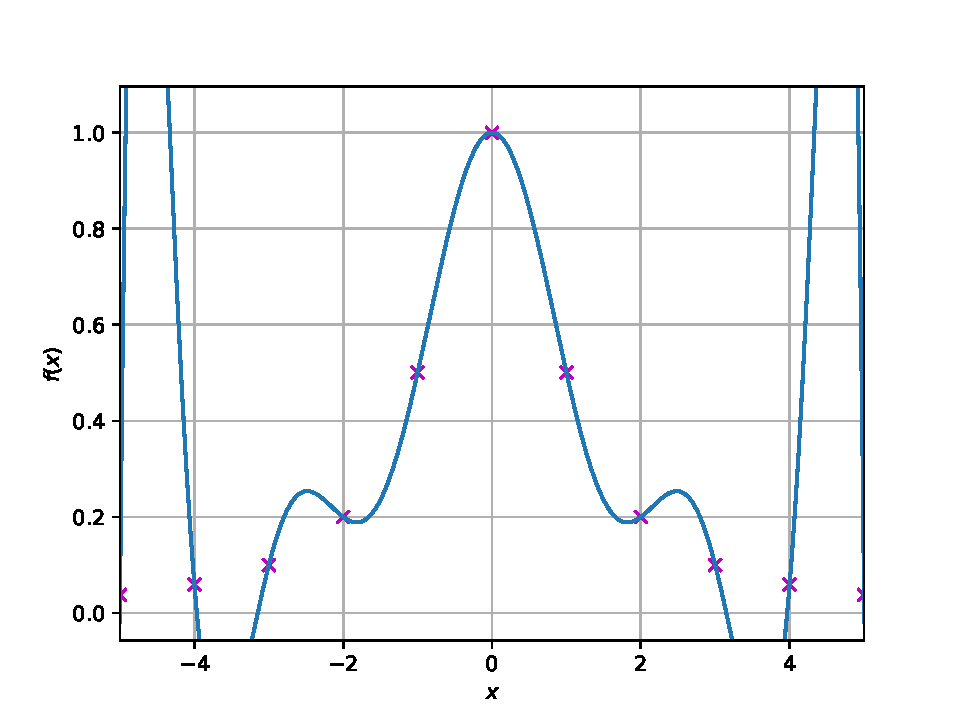
\includegraphics[width=0.35\textwidth]{runge1}&
\hspace*{-0.5cm}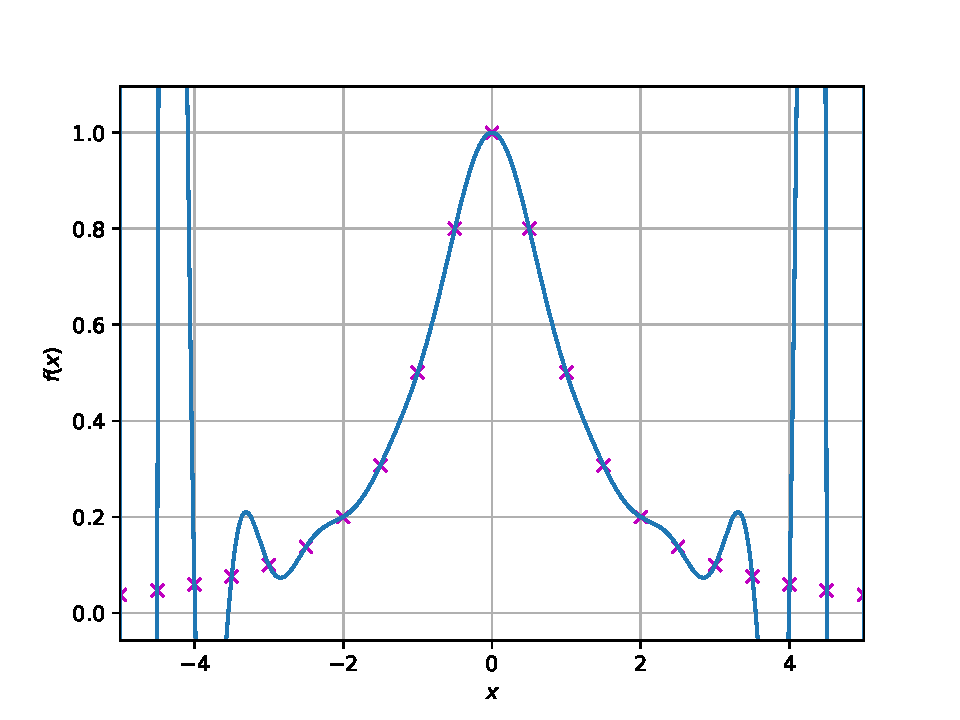
\includegraphics[width=0.35\textwidth]{runge2}&
\hspace*{-0.5cm}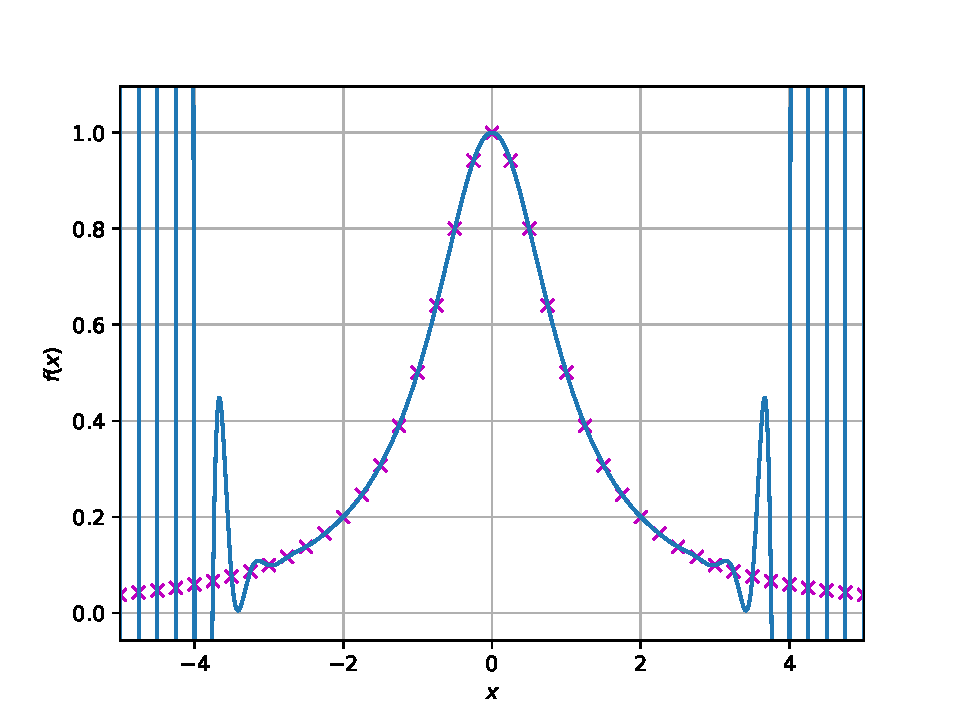
\includegraphics[width=0.35\textwidth]{runge3}\\
(a) & (b) & (c)\\
\end{tabular}
\caption{The Runge phenomenon on interpolating $f(x) = (1+x^2)^{-1}$ on $[-5,5]$: (a) using $11$ equispaced points (b) using $21$ equispaced points (c) using $41$ equispaced points.}
\label{figure:Runge}
\end{center}
\end{figure}

\begin{figure}[htbp]
\begin{center}
\begin{tabular}{ccc}
\hspace*{-0.5cm}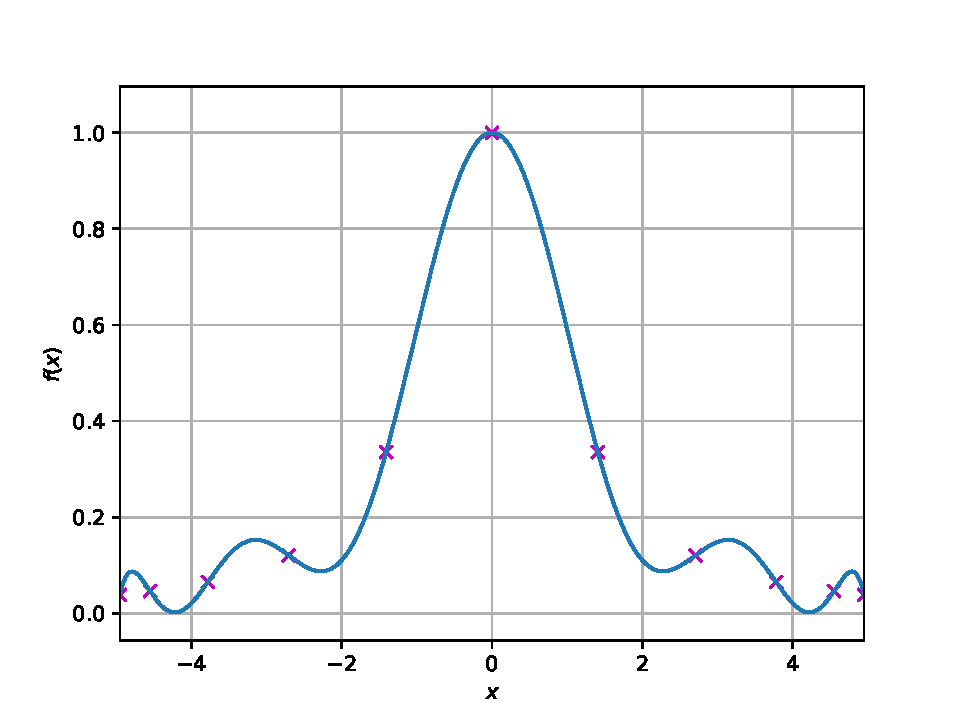
\includegraphics[width=0.35\textwidth]{rungefixed1}&
\hspace*{-0.5cm}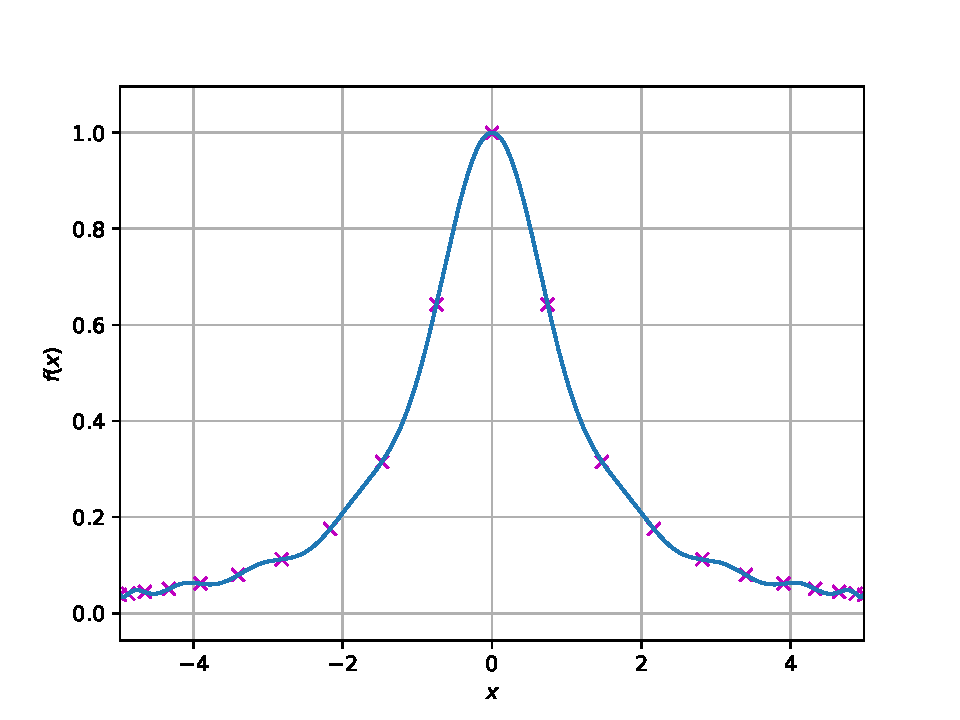
\includegraphics[width=0.35\textwidth]{rungefixed2}&
\hspace*{-0.5cm}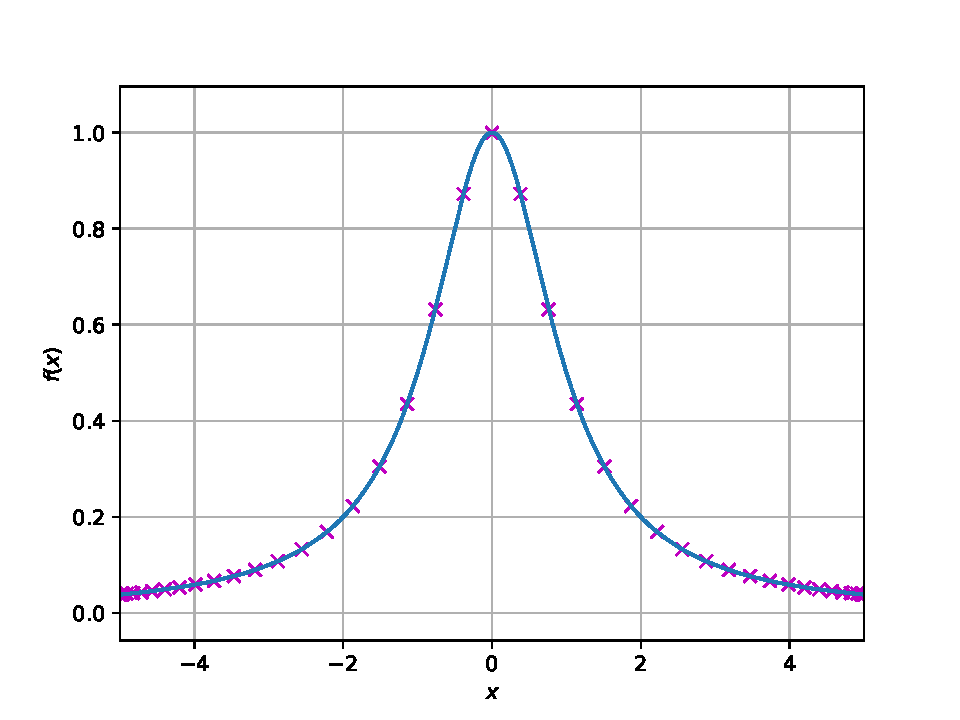
\includegraphics[width=0.35\textwidth]{rungefixed3}\\
(a) & (b) & (c)\\
\end{tabular}
\caption{Uniform convergence on interpolating $f(x) = (1+x^2)^{-1}$ on $[-5,5]$: (a) using $11$ Chebyshev points (b) using $21$ Chebyshev points (c) using $41$ Chebyshev points.}
\label{figure:RungeFixed}
\end{center}
\end{figure}

\section{Best Polynomial Approximation}

Given a function $f:D\to\C$, we wish to find its best polynomial approximation. To measure our progress, we can use $L^p(D,\ud\mu(x))$ spaces and their associated norms: find $p_n\in\P_n$ that is the best polynomial approximation to $f\in L^p(D,\ud\mu(x))$ such that:
\[
\|f-p_n\|_p \le \|f-q\|_p,\qquad\forall q\in\P_n.
\]
Posed in this generality, the problem is still the subject of ongoing research. Therefore, to make any reasonable progress, we will consider the solved problems of best approximation in $L^2$ followed by best approximation in $L^\infty$.

\subsection{Best Polynomial Approximation in $L^2$ and Orthogonal Polynomials}

We now consider the best polynomial approximations in $L^2(D,\ud\mu(x))$, i.e. find $p_n\in\P_n$ such that:
\[
\|f-p_n\|_2 \le \|f-q\|_2,\qquad\forall q\in\P_n.
\]
Supposing $p_n$ has the form $p_n(x) = \sum_{i=0}^n \alpha_i x^i$ then results in the minimization problem:
\[
\min_{(\alpha_0,\ldots,\alpha_n)\in\C^n} \int_D \abs{f(x)-\sum_{i=0}^n \alpha_i x^i}^2\ud\mu(x).
\]
The unique minimizer can be found from the (linear) system:
\[
\dfrac{\partial}{\partial\alpha_k}\int_D \abs{f(x)-\sum_{i=0}^n \alpha_i x^i}^2\ud\mu(x),\quad\hbox{for each}\quad k=0,\ldots,n.
\]
But there is some additional structure that we will exploit rather than solving this system of equations.

\begin{theorem}
If $f\in L^2(D,\ud\mu(x))$ and $p_n\in\P_n$ is such that:
\begin{equation}\label{eq:L2assumption}
\langle r,f-p_n\rangle = 0,\quad \forall r\in\P_n,
\end{equation}
then:
\begin{equation}
\|f-p_n\|_2 \le \|f-r\|_2,\quad \forall r\in\P_n,
\end{equation}
i.e. $p_n$ is a best (weighted) least-squares approximation to $f$ on $D$.
\end{theorem}
\begin{proof}
\begin{align*}
\|f-p_n\|_2^2 & = \abs{\langle f-p_n,f-p_n\rangle}\\
& = \abs{\langle f-r,f-p_n\rangle + \langle r-p_n,f-p_n\rangle},\quad \forall r\in\P_n.
\end{align*}
Since $r-p_n\in\P_n$, the assumption~\eqref{eq:L2assumption} implies that:
\begin{align*}
\|f-p_n\|_2^2 & = \abs{\langle f-r,f-p_n\rangle}\\
& \le \|f-r\|_2\|f-p_n\|_2,
\end{align*}
by the Cauchy--Schwarz inequality.
\end{proof}
\begin{remark}
The converse is also true.
\end{remark}

This gives a direct, albeit poor, way to calculate best polynomial approximations in $L^2$: we wish to find $p_n(x) = \sum_{i=0}^n \alpha_i x^i$ such that:
\begin{equation}
\int_D \conj{x^k}\br[f(x)-\sum_{i=0}^n \alpha_i x^i]\ud\mu(x) = 0,\quad{\rm for}\quad k=0,\ldots,n.
\end{equation}
Rearranging these equations, we have:
\begin{equation}
\sum_{i=0}^n\left(\int_D\conj{x^k}x^i\ud\mu(x)\right)\alpha_i = \int_D \conj{x^k}f(x)\ud\mu(x),\quad{\rm for}\quad k=0,\ldots,n,
\end{equation}
which is the component-wise statement of the matrix equation:
\begin{equation}\label{eq:normalequations}
A\alpha = \varphi,
\end{equation}
to determine the coefficients $\alpha = \pr(\alpha_0,\ldots,\alpha_n)^\top$ from the data $\varphi = \pr(\varphi_0,\ldots,\varphi_n)^\top$, where:
\begin{equation}
A_{k,i} = \int_D \conj{x^k}x^i\ud\mu(x),\quad{\rm and}\quad \varphi_k = \int_D \conj{x^k}f(x)\ud\mu(x).
\end{equation}
The system~\eqref{eq:normalequations} are called the {\bf normal equations}.

\begin{example}
We wish to find the best least-squares approximation to $e^x$ on $[0,1]$ from $\P_1$. We must solve:
\[
\int_0^1 1[e^x -(\alpha_0+\alpha_1x)]\ud x = 0,\quad{\rm and}\quad \int_0^1 x[e^x -(\alpha_0+\alpha_1x)]\ud x = 0.
\]
This is equivalent to:
\begin{align*}
\alpha_0\int_0^1\ud x + \alpha_1\int_0^1x\ud x & = \int_0^1 e^x\ud x,\\
\alpha_0\int_0^1x\ud x + \alpha_1\int_0^1x^2\ud x & = \int_0^1 e^xx\ud x,
\end{align*}
or:
\begin{align*}
\begin{bmatrix}
1 & \frac{1}{2}\\
\frac{1}{2} & \frac{1}{3}\\
\end{bmatrix}
\begin{bmatrix}
\alpha_0\\\alpha_1\\
\end{bmatrix}
\begin{bmatrix}
e-1\\1\\
\end{bmatrix},
\end{align*}
which has the solution $\alpha_0 = 4e-10$ and $\alpha_1 = 18-6e$. Therefore, $p_1(x) = (18-6e)x + (4e-10)$ is the best approximation to $e^x$ in $L^2([0,1],\ud x)$.
\end{example}

\begin{theorem}
The matrix $A$ in~\eqref{eq:normalequations} is nonsingular.
\end{theorem}
\begin{proof}
Suppose $A$ {\em is} singular, i.e. $\exists \alpha\ne 0$ such that $A\alpha = 0$ implying $\alpha^* A\alpha = 0$. This is:
\begin{equation}
\sum_{k=0}^n\conj{\alpha_k}(A\alpha)_k \Longleftrightarrow \sum_{k=0}^n\conj{\alpha_k}\sum_{i=0}^nA_{k,i}\alpha_i = 0.
\end{equation}
Since, by definition $A_{k,i} = \int_D \conj{x^k}x^i\ud\mu(x)$, we find:
\begin{equation}
\Longleftrightarrow \sum_{k=0}^n \conj{\alpha_k} \sum_{i=0}^n \int_D \conj{x^k}x^i\ud\mu(x) \alpha_i = 0.
\end{equation}
Rearranging gives:
\begin{equation}
\int_D\conj{\pr(\sum_{k=0}^n \alpha_kx^k)}\pr(\sum_{i=0}^n \alpha_ix^i)\ud\mu(x) = 0,\quad{\rm or}\quad \left\|\sum_{i=0}^n \alpha_i x^i\right\|_2^2 = 0.
\end{equation}
But this last equality implies that $\sum_{i=0}^n\alpha_ix^i\equiv0$ and thus $\alpha_i\equiv0$ for $i=0,\ldots,n$. We have arrived at a contradiction.
\end{proof}
Invertibility of the matrix $A$ establishes existence and uniqueness of the best polynomial approximation in $L^2(D,\ud\mu(x))$. It does not, however, imply that the normal equations are well-conditioned. To find a well-conditioned solution to this problem, we use our knowledge of the QR factorization for matrices to construct degree-graded polynomial bases that behave significantly better than the monomials.

The solution of the normal equations $A\alpha = \varphi$ for best least-squares polynomial approximation would be trivial if $A$ were diagonal. Instead of using $\{1,x,\ldots,x^n\}$ as a basis for $\P_n$, we shall construct a basis $\{\pi_0,\pi_1,\ldots,\pi_n\}$ in order to diagonalize $A$.

In this basis, our best polynomial approximation $p_n(x) = \sum_{i=0}^n \beta_i\pi_i(x)$, and the normal equations become:
\begin{equation}
\int_D\conj{\pi_k(x)}\br[f(x)-\sum_{i=0}^n\beta_i\pi_i(x)]\ud\mu(x) = 0,\quad{\rm for}\quad k=0,\ldots,n,
\end{equation}
or equivalently:
\[
\sum_{i=0}^n\left(\int_D\conj{\pi_k(x)}\pi_i(x)\ud\mu(x)\right)\beta_i = \int_D\conj{\pi_k(x)}f(x)\ud\mu(x),\quad{\rm for}\quad k=0,\ldots,n,
\]
or:
\begin{equation}
A\beta = \varphi,
\end{equation}
where $\beta = \pr(\beta_0,\ldots,\beta_n)^\top$, $\varphi = \pr(\varphi_0,\ldots,\varphi_n)^\top$ but now:
\begin{equation}
A_{k,i} = \langle \pi_k, \pi_i \rangle = \int_D \conj{\pi_k(x)}\pi_i(x)\ud\mu(x),\quad{\rm and}\quad \varphi_k = \int_D \conj{\pi_k(x)}f(x)\ud\mu(x).
\end{equation}
The matrix $A$ is diagonalized iff:
\[
\langle \pi_k, \pi_i \rangle ~\left\{\begin{array}{ccc} = 0 & \for & i\ne k,\\ \ne 0 & \for & i = k.\end{array}\right.
\]
We can use this (countably infinite) set of conditions to construct the {\bf orthogonal polynomials} with respect to the measure $\ud\mu(x)$. This is known as the Gram--Schmidt procedure.

\begin{lemma} Suppose that $\pi_0,\ldots,\pi_k,$ with $\pi_i\in\P_i$ for each $i$, are orthogonal with respect to the inner product $\langle f,g\rangle = \int_D\conj{f(x)}g(x)\ud\mu(x)$. Then:
\[
\pi_{k+1}(x) = x^{k+1} - \sum_{i=0}^k\delta_i\pi_i(x),
\]
satisfies:
\[
\langle \pi_{j},\pi_{k+1} \rangle = 0,\quad{\rm for}\quad j=0,\ldots,k,\quad{\and}\quad \delta_j = \dfrac{\langle \pi_j,x^{k+1}\rangle}{\langle\pi_j,\pi_j\rangle}.
\]
\end{lemma}
\begin{proof}
For any $j=0,\ldots,k$,
\begin{align*}
\langle\pi_j,\pi_{k+1}\rangle & = \langle \pi_j,x^{k+1}\rangle - \sum_{i=0}^k \delta_i \langle \pi_j,\pi_i\rangle\\
& = \langle \pi_j,x^{k+1}\rangle - \delta_j \langle \pi_j,\pi_j\rangle\quad\hbox{by orthogonality of $\pi_i$ and $\pi_j$ for $i\ne j$},\\
& = 0,\quad\hbox{by definition of $\delta_j$.}
\end{align*}
\end{proof}

\begin{remark}
The Gram--Schmidt procedure constructs orthogonal polynomials inductively starting from $\pi_0(x) = 1$. $\pi_k(x)$ is always of exact degree $k$, so $\{\pi_0,\ldots,\pi_k\}$ is a basis for $\P_k$, $\forall k\in\N_0$. The orthogonal polynomials can be normalized to be {\bf orthonormal}, i.e. $\langle\pi_k,\pi_k\rangle = 1$, to be {\bf monic}, i.e. $\hat{\pi}_k(x) = x^k + \cdots +$, or even have other normalizations such as $\pi_k(1)=1$.
\end{remark}

\subsubsection{Properties of Orthogonal Polynomials}

In order to provide a basis for computational techniques associated with the preceding approximations, as well as for later developments, we next exhibit some useful properties of orthogonal polynomials.

\begin{theorem}\label{theorem:OPzeros}
For every $n\in\N$ and $a,b\in\R$, if the measure $\mu$ is monotonic, the orthogonal polynomials $\pi_n$ with respect to $L^2([a,b],\ud\mu(x))$ possess $n$ distinct real zeros contained in $(a,b)$.
\end{theorem}
\begin{proof}
If $\pi_n$ does not change in sign in $[a,b]$, then:
\[
\int_a^b\pi_n\ud\mu(x) = \langle \pi_0,\pi_n\rangle,
\]
is either positive or negative. In either case, this is a contradiction since the right-hand side must be zero by orthogonality. Hence, $\pi_n$ must have a zero in $(a,b)$. Now, let those real zeros of $\pi_n(x)$ which are of {\em odd} multiplicity, and which lie in $(a,b)$, be denoted by $x_1, x_2,\ldots, x_m,$ and {\em assume} that $m<n$. Then the product:
\[
(x-x_1)(x-x_2)\cdots(x-x_m)\pi_n(x),
\]
does not change sign in $[a,b]$. Since $m<n$, the product $(x-x_1)\cdots(x-x_m)$ is a polynomial of degree less than $n$ and it may be expressed in terms of the basis $\{\pi_k(x)\}_{k=0}^m$. We must have:
\begin{equation}\label{eq:MonotonicOP}
\langle (x-x_1)(x-x_2)\cdots(x-x_m),\pi_n(x)\rangle = 0.
\end{equation}
However, since the measure is monotonic in $[a,b]$, the integrand therefore has the same property, and we have reached a contradiction, as this guarantees that~\eqref{eq:MonotonicOP} must be different from $0$. Hence, it follows that $m=n$, and since the total multiplicity of {\em all} zeros is equal to $n$, all roots must be real and distinct and must lie in $(a,b)$.
\end{proof}

\begin{theorem}\label{theorem:threetermrecurrence}
For every $n\in\N$, the monic orthogonal polynomials $\hat{\pi}_n$ with respect to $L^2([a,b],\ud\mu(x))$ satisfy a three-term recurrence relation of the form:
\begin{equation}\label{eq:threetermrecurrence}
\hat{\pi}_{n+1}(x) = (x-\alpha_n)\hat{\pi}_n(x) - \beta_n\hat{\pi}_{n-1}(x).
\end{equation}
\end{theorem}
\begin{proof}
The case $n=1$ holds trivially. Assume the result holds for $n-1$. Since $\hat{\pi}_{n+1}-x\hat{\pi}_n\in\P_n$ and since $\{\hat{\pi}_0,\ldots,\hat{\pi}_n\}$ is a basis for $\P_n$, it follows that:
\[
\hat{\pi}_{n+1}(x) - x\hat{\pi}_n(x) = -\alpha_n\hat{\pi}_n(x) - \beta_n\hat{\pi}_{n-1} - \sum_{j=0}^{n-2}\gamma_j\hat{\pi}_j(x),
\]
for some constants $\alpha_n$, $\beta_n$, and $\gamma_j$. If we take the inner product with $\hat{\pi}_n$, we obtain:
\[
0 - \langle x\hat{\pi}_n,\hat{\pi}_n\rangle = -\alpha_n\langle\hat{\pi}_n,\hat{\pi}_n\rangle \quad{\rm or}\quad \alpha_n = \dfrac{\langle x\hat{\pi}_n,\hat{\pi}_n\rangle}{\langle\hat{\pi}_n,\hat{\pi}_n\rangle}.
\]
Next, if we take the inner product with $\hat{\pi}_{n-1}$, we obtain:
\[
0 - \langle x\hat{\pi}_n,\hat{\pi}_{n-1}\rangle = -\beta_n\langle\hat{\pi}_{n-1},\hat{\pi}_{n-1}\rangle \quad{\rm or}\quad \beta_n = \dfrac{\langle x\hat{\pi}_n,\hat{\pi}_{n-1}\rangle}{\langle\hat{\pi}_{n-1},\hat{\pi}_{n-1}\rangle} = \dfrac{\langle \hat{\pi}_n,x\hat{\pi}_{n-1}\rangle}{\langle\hat{\pi}_{n-1},\hat{\pi}_{n-1}\rangle} = \dfrac{\langle \hat{\pi}_n,\hat{\pi}_n\rangle}{\langle\hat{\pi}_{n-1},\hat{\pi}_{n-1}\rangle}.
\]
Finally, any of the inner products with $\hat{\pi}_j$ for $j=0,\ldots,n-2$ give:
\[
0 - \langle x\hat{\pi}_n,\hat{\pi}_{j}\rangle = -\gamma_j\langle\hat{\pi}_{j},\hat{\pi}_{j}\rangle.
\]
Since $\deg(x\hat{\pi}_j) = j+1 < n$, each of the $\gamma_j=0$.
\end{proof}

Without loss of generality, orthogonal polynomials $\pi_n$ with any normalization (not necessarily monic) satisfy a three-term recurrence relation. Consider then the notation:
\begin{equation}\label{eq:OPrec}
\pi_{n+1}(x) = (A_nx+B_n)\pi_n(x) -C_n\pi_{n-1}(x),\qquad \pi_{-1}(x) = 0,\quad \pi_0(x) = 1.
\end{equation}
The following algorithm is the extension of Horner's rule for numerical evaluation of polynomials expressed in general orthogonal polynomial bases. The Clenshaw--Smith algorithm writes the sum:
\begin{equation}
p_n(x) = \sum_{k=0}^n c_k \pi_k(x),
\end{equation}
via an inhomogeneous recurrence relation involving the adjoint of~\eqref{eq:OPrec} as follows:
\begin{algorithm}[Clenshaw--Smith~\cite{Clenshaw-9-118-55,Smith-19-33-65}]~
\begin{enumerate}
\item Set:
\begin{equation}
u_{n+1}(x) = u_{n+2}(x) = 0.
\end{equation}
\item For $k=n,n-1,\ldots,0$:
\begin{equation}
u_k(x) = (A_kx+B_k)u_{k+1}(x) - C_{k+1}u_{k+2}(x) + c_k.
\end{equation}
\item Then:
\begin{equation}
p_n(x) = u_0(x).
\end{equation}
\end{enumerate}
\end{algorithm}

The Clenshaw--Smith allows for numerical evaluation of polynomials expressed in orthogonal bases in $\OO(n)$ flops with $\OO(1)$ storage.

\begin{theorem}\label{theorem:ChristoffelDarboux}
Let $\tilde{\pi}_n$ represent the orthonormal polynomials with respect to $L^2([a,b],\ud\mu(x))$. Then, the Christoffel--Darboux formula is:
\begin{equation}\label{eq:ChristoffelDarboux}
\sum_{k=0}^{n-1}\tilde{\pi}_k(x)\tilde{\pi}_k(y) = \sqrt{\beta_n}\dfrac{\tilde{\pi}_n(x)\tilde{\pi}_{n-1}(y) - \tilde{\pi}_{n-1}(x)\tilde{\pi}_n(y)}{x-y}.
\end{equation}
\end{theorem}
\begin{proof}
Multiplying the three-term recurrence relation~\eqref{eq:threetermrecurrence} by $\hat{\pi}_k(y)$ and subtracting the resulting relation from the one with $x$ and $y$ interchanged yields:
\[
(x-y)\hat{\pi}_k(x)\hat{\pi}_k(y) = \beta_k\hat{\pi}_{k-1}(x)\hat{\pi}_k(y) - \beta_k \hat{\pi}_k(x)\hat{\pi}_{k-1}(y) + \hat{\pi}_{k+1}(x)\hat{\pi}_k(y) - \hat{\pi}_k(x)\hat{\pi}_{k+1}(y).
\]
Recall that $\beta_k = \frac{\langle \hat{\pi}_k,\hat{\pi}_k\rangle}{\langle\hat{\pi}_{k-1},\hat{\pi}_{k-1}\rangle}$. So this relation is equivalent to:
\begin{align*}
(x-y)\dfrac{\hat{\pi}_k(x)\hat{\pi}_k(y)}{\langle \hat{\pi}_k,\hat{\pi}_k\rangle} & = \dfrac{\hat{\pi}_{k-1}(x)\hat{\pi}_k(y)}{\langle\hat{\pi}_{k-1},\hat{\pi}_{k-1}\rangle} - \dfrac{\hat{\pi}_k(x)\hat{\pi}_{k-1}(y)}{\langle\hat{\pi}_{k-1},\hat{\pi}_{k-1}\rangle}\\ & - \dfrac{\hat{\pi}_k(x)\hat{\pi}_{k+1}(y)}{\langle \hat{\pi}_k,\hat{\pi}_k\rangle} + \dfrac{\hat{\pi}_{k+1}(x)\hat{\pi}_k(y)}{\langle \hat{\pi}_k,\hat{\pi}_k\rangle}.
\end{align*}
Summing both sides from $k=0$ to $k=n-1$ and observing $\hat{\pi}_{-1}\equiv0$ and the telescoping nature of the summation on the right gives:
\[
\sum_{k=0}^{n-1} \dfrac{\hat{\pi}_k(x)\hat{\pi}_k(y)}{\langle \hat{\pi}_k,\hat{\pi}_k\rangle} = \dfrac{1}{\langle \hat{\pi}_{n-1},\hat{\pi}_{n-1}\rangle} \dfrac{\hat{\pi}_n(x)\hat{\pi}_{n-1}(y) - \hat{\pi}_{n-1}(x)\hat{\pi}_n(y)}{x-y}.
\]
Equation~\eqref{eq:ChristoffelDarboux} only requires orthonormalization.
\end{proof}

\subsubsection{The Classical Orthogonal Polynomials}

The classical orthogonal polynomials are all eigenfunctions of linear second-order homogeneous differential equations of the form:
\begin{equation}
Q(x)\pi_n''(x) + L(x)\pi_n'(x) = \lambda_n\pi_n(x),
\end{equation}
where $Q\in\P_2$ and $L\in\P_1$, and where the eigenvalues are given by $\lambda_n = nL'(x) +\dfrac{n(n-1)}{2}Q''(x)$. With this extra structure, an explicit representation in terms of higher order derivatives can be derived.
\begin{theorem}[p. 24 of Nikiforov and Uvarov~\cite{Nikiforov-Uvarov-88}]\label{theorem:Rodrigues}
The classical orthogonal polynomials $\pi_n\in\P_n$ with respect to the inner product space $L^2(D,w(x)\ud x)$ can be expressed by {\bf Rodrigues' formula}:
\begin{equation}
\pi_n(x) = \dfrac{1}{\kappa_n w(x)}\dfrac{\ud^n}{\ud x^n}\left(w(x)(Q(x))^n\right).
\end{equation}
\end{theorem}

\begin{example}
The Legendre polynomials, denoted by $P_n(x)$, are orthogonal with respect to $L^2(\I,\ud x)$ and are normalized by $P_n(1)=1$. They satisfy the differential equation:
\begin{equation}
(1-x^2)\pi_n''(x) -2x\pi_n'(x) + n(n+1)\pi_n(x) = 0,
\end{equation}
and therefore, Rodrigues' formula states that:
\begin{equation}
P_n(x) = \dfrac{1}{(-2)^nn!}\dfrac{\ud^n}{\ud x^n}\left(1-x^2\right)^n.
\end{equation}
\end{example}

\begin{example}
The Chebyshev polynomials of the first kind, denoted by $T_n(x)$, are orthogonal with respect to $L^2(\I,(1-x^2)^{-\frac{1}{2}}\ud x)$ and are normalized by $T_n(1)=1$. By making the variable transformation $x=\cos\theta$, the inner product becomes:
\[
\langle \pi_k,\pi_j\rangle = \int_0^\pi \pi_k(\cos\theta)\pi_j(\cos\theta)\ud\theta.
\]
Explicitly:
\begin{equation}\label{eq:Tn}
T_n(\cos\theta) = \cos(n\theta),\quad{\rm or}\quad T_n(x) = \cos(n\cos^{-1}(x)).
\end{equation}
\end{example}

\begin{example}
The Chebyshev polynomials of the second kind, denoted by $U_n(x)$, are orthogonal with respect to $L^2(\I,\sqrt{1-x^2}\ud x)$ and normalized by $U_n(1)=n+1$. By making the variable transformation $x=\cos\theta$, the inner product becomes:
\[
\langle \pi_k,\pi_j\rangle = \int_0^\pi \pi_k(\cos\theta)\pi_j(\cos\theta)\sin^2\theta\ud\theta.
\]
Explicitly:
\begin{equation}
U_n(\cos\theta) = \dfrac{\sin((n+1)\theta)}{\sin\theta},\quad{\rm or}\quad U_n(x) = \dfrac{\sin((n+1)\cos^{-1}(x))}{\sqrt{1-x^2}}.
\end{equation}
\end{example}

Table~\ref{table:ClassicalOrthogonalPolynomials} describes the classical orthogonal polynomials. Note that Legendre and Chebyshev polynomials are special cases of Jacobi polynomials. Figure~\ref{figure:TUP} shows the first six polynomials $T_n(x)$, $U_n(x)$, and $P_n(x)$.

\begin{table}[htdp]
\caption{The classical orthogonal polynomials}
\begin{center}
\begin{tabular}{cccc}
\sphline
Name & Jacobi & Laguerre & Hermite\\
\sphline
Notation & $P_n^{(\alpha,\beta)}(x)$ & $L_n(x)$ & $H_n(x)$\\
\sphline
Domain & $\I$ & $[0,\infty)$ & $\R$\\
\sphline
$w(x)$ & $(1-x)^\alpha(1+x)^\beta$ & $e^{-x}$ & $e^{-x^2}$\\
$A_n$ & $\dfrac{(2n+\alpha+\beta+1)(2n+\alpha+\beta+2)}{2(n+1)(n+\alpha+\beta+1)}$ & $-\dfrac{1}{n+1}$ & $2$\\
$B_n$ & $\dfrac{(\alpha^2-\beta^2)(2n+\alpha+\beta+1)}{2(n+1)(n+\alpha+\beta+1)(2n+\alpha+\beta)}$ & $\dfrac{2n+1}{n+1}$ & $0$\\
$C_n$ & $\dfrac{(n+\alpha)(n+\beta)(2n+\alpha+\beta+2)}{(n+1)(n+\alpha+\beta+1)(2n+\alpha+\beta)}$ & $\dfrac{n}{n+1}$ & $2n$\\
$Q(x)$ & $1-x^2$ & $x$ & $1$\\
$\kappa_n$ & $(-2)^nn!$ & $n!$ & $(-1)^n$\\
\sphline
\end{tabular}
\end{center}
\label{table:ClassicalOrthogonalPolynomials}
\end{table}%

\begin{figure}[htbp]
\begin{center}
\begin{tabular}{ccc}
\hspace*{-0.5cm}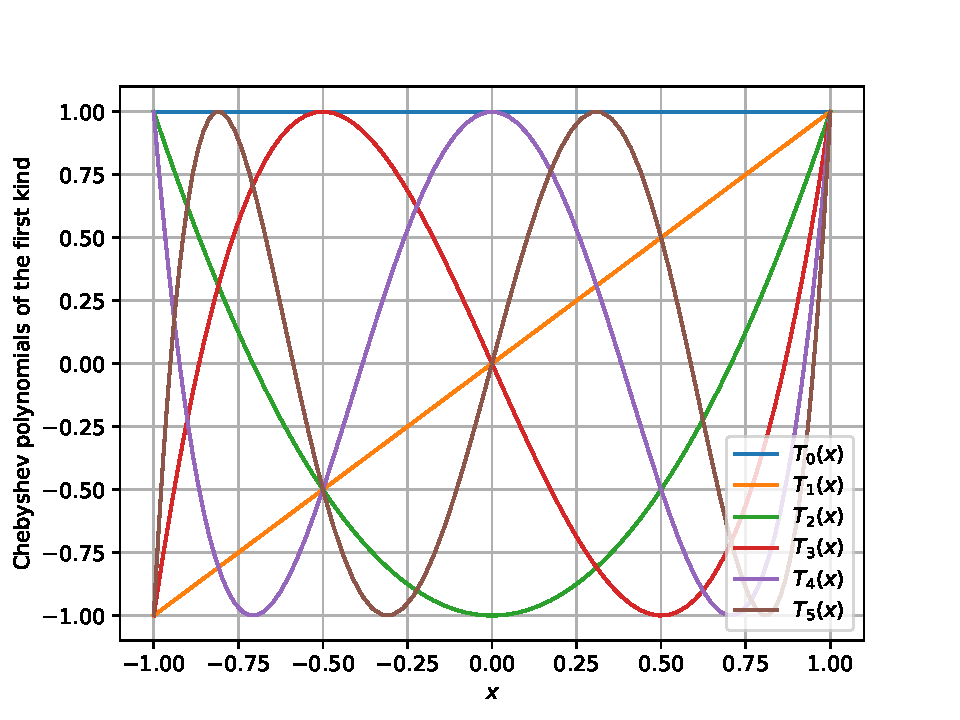
\includegraphics[width=0.35\textwidth]{chebyshevt}&
\hspace*{-0.5cm}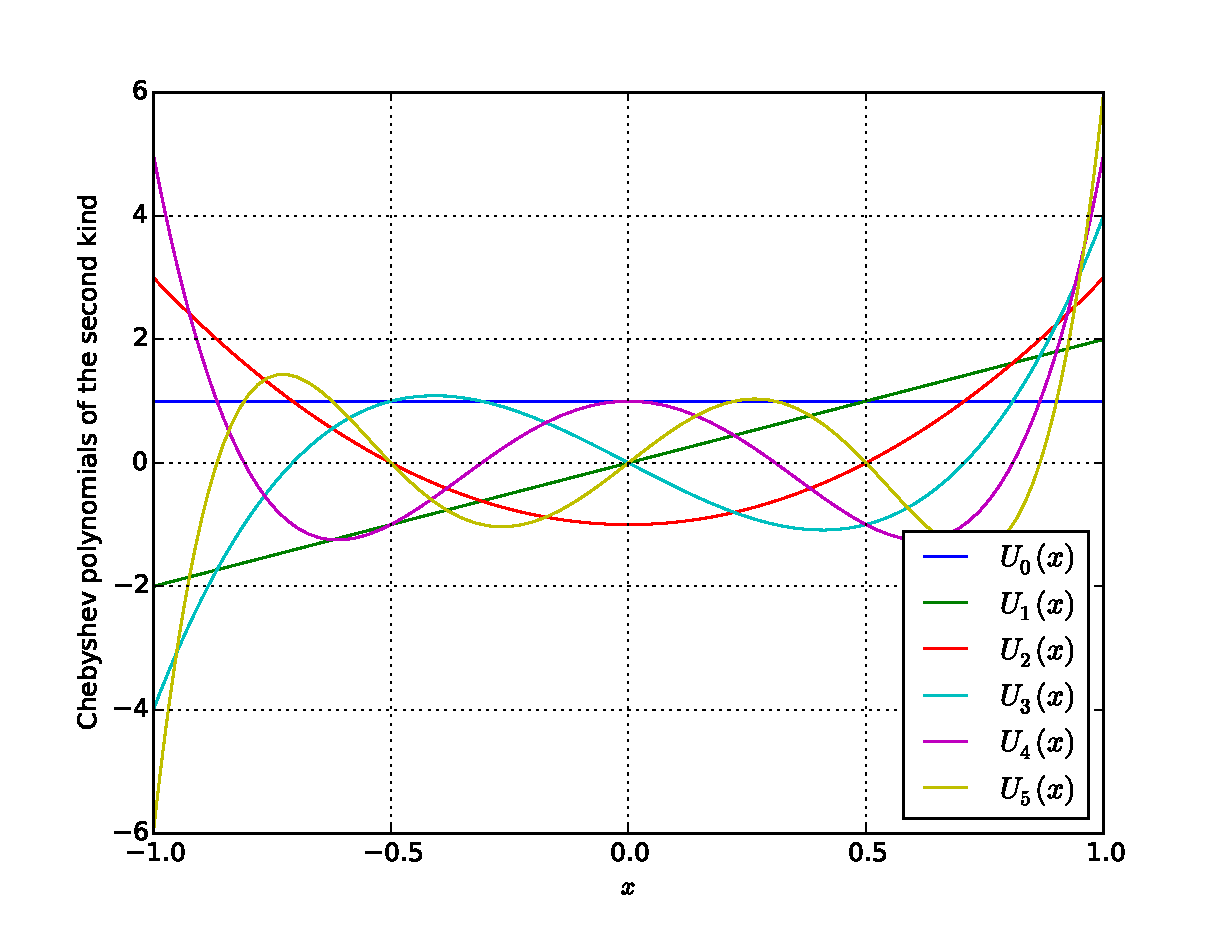
\includegraphics[width=0.35\textwidth]{chebyshevu}&
\hspace*{-0.5cm}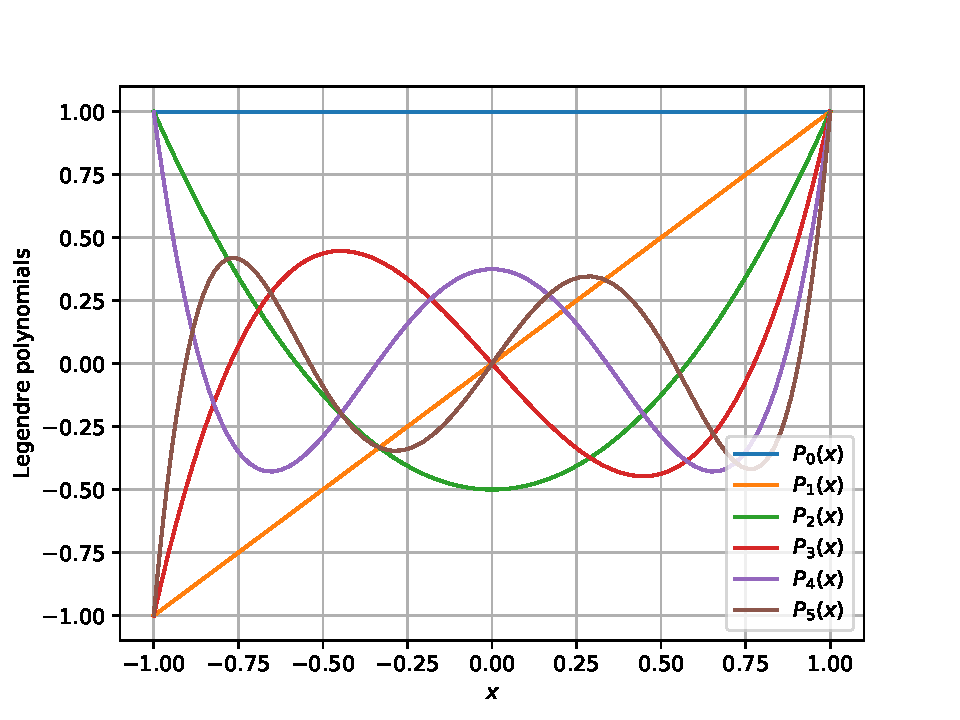
\includegraphics[width=0.35\textwidth]{legendre}\\
(a) & (b) & (c)\\
\end{tabular}
\caption{The first six Chebyshev polynomials of the (a) first kind, (b) second kind, and (c) Legendre polynomials.}
\label{figure:TUP}
\end{center}
\end{figure}

\subsection{Best Polynomial Approximation in $L^\infty$ and The Remez Exchange Algorithm}

We have seen that best polynomial approximation in $L^2$ is a rich and well-developed subject. Best polynomial approximation in $L^\infty$ is just as fascinating, though as the results will show, it is hardly as practical. It turns out that best polynomial approximation in $L^\infty$ is an old idea dating from the time of Chebyshev and Poncelet.

In this section, we consider the best polynomial approximations in $L^\infty([a,b])$, i.e. find $p_n\in\P_n$ such that:
\[
\|f-p_n\|_\infty \le \|f-q\|_\infty,\qquad\forall q\in\P_n.
\]
The main result of this section is to characterize the polynomials of best approximation as {\bf alternants}.
\begin{theorem}[Chap.~10 in Trefethen~\cite{Trefethen-12}]\label{theorem:Equioscillation}
Every $f\in C([a,b])$ has a unique best approximation $p_n\in\P_n$. If $f$ is real, then $p_n$ is real, and in this case a polynomial $q\in\P_n$ is equal to $p_n$ if and only if $f-q$ equioscillates in at least $n+2$ extreme points.
\end{theorem}
\begin{proof}
We partition the proof.
\begin{description}
\item[Existence] We note that $\|f-q\|_\infty$ is a continuous function of $q\in\P_n$. Since one candidate approximation is the zero function, we know that if $p_n$ exists, it lies in $\{q\in\P_n : \|f-q\|_\infty \le \|f\|_\infty\}$. This is a closed and bounded subset of a finite-dimensional space, hence compact (the Bolzano-Weierstrass property), and thus the minimum is attained.
\item[Equioscillation $\Longrightarrow$ optimality] Suppose $f$ and $p$ are real and $(f-p)(x)$ takes equal extreme values with alternating signs at $n+2$ points $x_0<\cdots<x_{n+1}$, and suppose $\|f-q\|_\infty < \|f-p\|_\infty$ for some real polynomial $q\in\P_n$. Then $p-q$ must take nonzero values with alternating signs at the equisocillation points, implying that it takes the value zero in at least $n+1$ points in between. This implies that $p-q\equiv0$, which is a contradiction.
\item[Optimality $\Longrightarrow$ equioscillation] Suppose $f-p$ equioscillates at fewer than $n+2$ points, and set $e = \|f-p\|_\infty$. Without loss of generality, suppose the leftmost extremum is one where $f-p = -e$. Then there are numbers $a < x_1 < \cdots < x_k < b$ with $k\le n$ such that $(f-p)(x) < e$ for $x\in[a,x_1]\cup[x_2,x_3]\cup[x_4,x_5]\cup\cdots\cup$ and $(f-p)(x)>-e$ for $x\in[x_1,x_2]\cup[x_3,x_4]\cup\cdots\cup$. If we define $\delta p(x) := (x_1-x)(x_2-x)\cdots(x_k-x)$, then $(p-\varepsilon\delta p)(x)$ will be a better approximation than $p$ to $f$ for all sufficiently small $\varepsilon>0$.
\item[Uniqueness] Suppose $p$ is a best approximation with equioscillation extrema $x_0<x_1<\cdots<x_{n+1}$, and suppose $\|f-q\|_\infty \le \|f-p\|_\infty$ for some real polynomial $q\in\P_n$. Then, without loss of generality, $(p-q)(x)$ must be nonpositive at $x_0,x_2,x_4,\ldots,$ and nonnegative at $x_1,x_3,x_5,\ldots.$ This implies that $p-q$ has roots in each of the $n+1$ closed intervals $[x_0,x_1], [x_1,x_2],\ldots,[x_n,x_{n+1}]$. We wish to conclude that $p-q$ has at least $n+1$ roots in total, counted with multiplicity, implying that $p=q$. To make the argument we prove by induction that $p-q$ has at least $k$ roots in $[x_0,x_k]$ for each $k$. The case $k=1$ is immediate. For the general case, suppose that $p-q$ has at least $j$ roots in $[x_0,x_j]$ for each $j\le k-1$ but only $k-1$ roots in $[x_0,x_k]$. Then there must be a simple root at $x_{k-1}$. By the induction hypothesis, $p-q$ must have exactly $k-2$ roots in $[x_0,x_{k-2}]$ with a simple root at $x_{k-2}$, $k-3$ roots in $[x_0,x_{k-3}]$ with a simple root at $x_{k-3}$, and so on down to one root in $[x_0,x_1]$, with a simple root at $x_1$. It follows that $p-q$ must be nonzero at $x_0$ and at $x_k$, and since the sign of $p-q$ changes at each of the simple roots $x_1,\ldots,x_{k-1},$ the signs at $x_0$ and $x_k$ must be the same if $k$ is odd and opposite if $k$ is even. On the other hand, from the original alternation condition, we know that $p-q$ must take the same signs at $x_0$ and at $x_k$ if $k$ is even and opposite signs if $k$ is odd.
\end{description}
\end{proof}

Theorem~\ref{theorem:Equioscillation} provides the mathematical foundation for the Remez exchange algorithm, the algorithm that iteratively computes best polynomial approximations in $L^\infty([a,b])$.

\begin{algorithm}\label{algorithm:Remez} The Remez exchange algorithm on $[-1,1]$. Let $p_n(x) = \sum_{k=0}^n c_kT_k(x)$.
\begin{enumerate}
\item Given the points $-1\le x_0<\cdots<x_{n+1}\le1$, solve the linear system of $n+2$ equations:
\[ c_0 + c_1 T_1(x_i) + \cdots + c_nT_n(x_i) + (-1)^ie = f(x_i)\quad{\rm for}\quad i=0,\ldots,n+1,
\]
for the unknowns $c_0,\ldots,c_n$ and $e$.
\item Improve upon the points $x_0<\cdots<x_{n+1}$ and their errors $\pm e$ by finding the local maxima:
\[
\bar{x}_k = \argmax_{x\in(x_{k-1},x_{k+1})}|f(x)-p_n(x)|,\quad{\rm for}\quad k=1,\ldots,n,
\]
and expect $x_0=a$ and $x_{n+1}=b$.
\item Define $z_i := |f(\bar{x}_i)-p_n(\bar{x}_i)|$ for $i=0,\ldots,n+1$. Then with $z_{\min} := \min\{z_i\}$ and $z_{\max} := \max\{z_i\}$ as lower and upper bounds for the best approximation errors, iterate until $z_{\min} \approx z_{\max}$ in the working precision.
\end{enumerate}
\end{algorithm}
The best polynomial approximation is represented in the basis of the Chebyshev polynomials of the first kind so as to render the system as well-conditioned as possible. As simple variable transformation allows for the algorithm to be applied to the general interval $[a,b]$. The Chebyshev nodes are a common choice for the initial set of points because Chebyshev polynomial interpolants give near-best polynomial approximants in $L^\infty([-1,1])$.

Figure~\ref{figure:Remez} shows the approximants generated by the Remez algorithm to the continuous function $f(x) = |x+\tfrac{1}{2}|$.

\begin{figure}[htbp]
\begin{center}
\begin{tabular}{cc}
\hspace*{-0.5cm}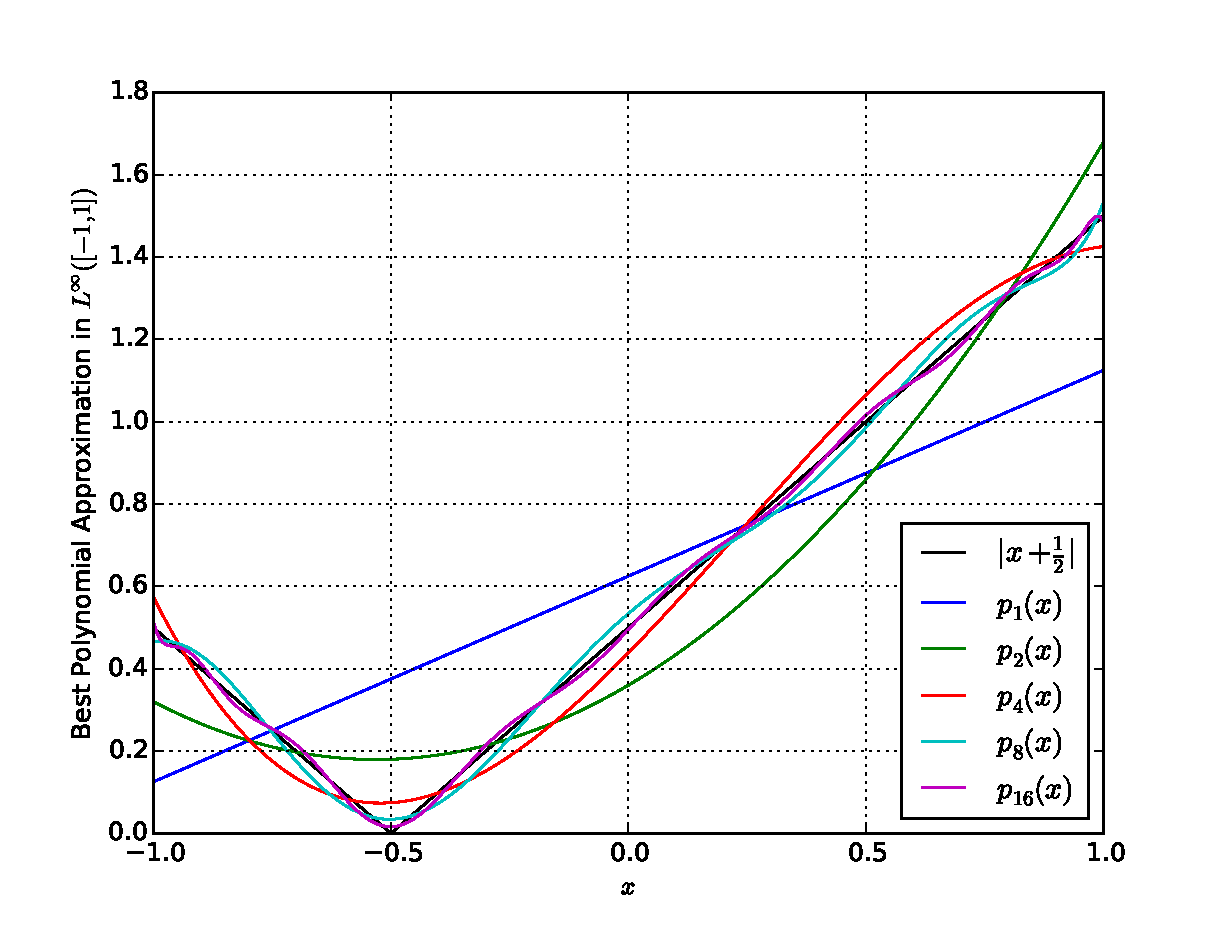
\includegraphics[width=0.525\textwidth]{BPAabs}&
\hspace*{-0.5cm}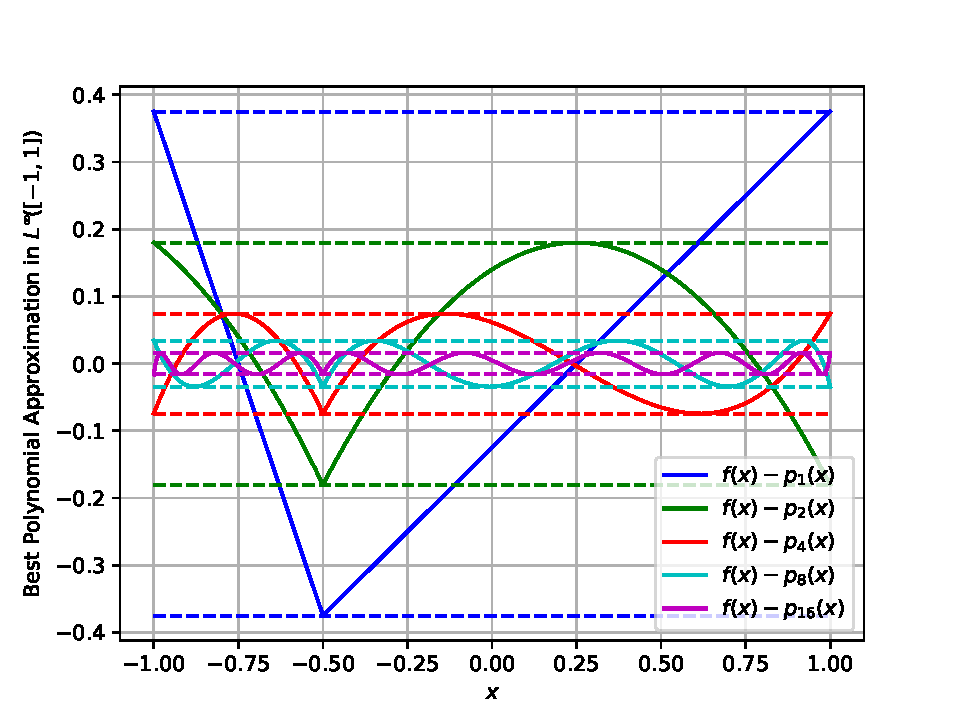
\includegraphics[width=0.525\textwidth]{BPAerrabs}\\
(a) & (b)\\
\end{tabular}
\caption{The Remez algorithm for best polynomial approximation to the continuous function $f(x) = |x+\tfrac{1}{2}|$ on $[-1,1]$: (a) the function and the polynomial approximants (b) the error, showing equioscillation.}
\label{figure:Remez}
\end{center}
\end{figure}


\subsection{The Best Choice of Interpolation Nodes on $\I$}\label{subsection:ChebyshevPointsAreTheBest}

We have now studied Lagrange interpolation; we have seen how best polynomial approximation in $L^2$ leads to the beautiful theory of orthogonal polynomials; and, we have examined the more complicated task of best polynomial approximation in $L^\infty$. We now have all the necessary tools to eliminate the Runge phenomenon that was depicted in Figure~\ref{figure:Runge}. Given the remainder Theorem~\ref{theorem:LagrangeInterpolatingRemainder}, we know that for sufficiently smooth functions, the remainder is given by:
\[
r(x) = f(x)-p_n(x) = \ell(x)\dfrac{f^{(n+1)}(\xi)}{(n+1)!}.
\]
In an effort to obtain uniformly convergent interpolating polynomials, one may ask how best to choose the interpolation points $x_0,\ldots,x_n$. Since the function $\ell(x) = \prod_{i=0}^n(x-x_i)$, we may ask which set of points will minimize the uniform norm:
\[
\inf_{(x_0,\ldots,x_n)\in\I}\|\ell\|_\infty?
\]
This question is answered by the following theorem.
\begin{theorem}
The Chebyshev points of the first kind (i.e. the roots of $T_n(x)$) infimize the norm $\|\ell\|_\infty$ on $\I$.
\end{theorem}
\begin{proof}
From~\eqref{eq:Tn}, it is clear that the Chebyshev polynomials of the first kind have unit uniform norm, $\|T_n\|_\infty = 1$. Furthermore, they {\em equioscillate} between their $n+1$ extrema. Invoking Theorem~\ref{theorem:Equioscillation}, we now see that $T_n$ are the errors associated with {\em best polynomial approximations} (to wit $f(x) = x^n$ and $p_n(x) = x^n-T_n(x)$), and thus infimize the norm. Since $\ell(x)$ is monic, and since the coefficient of $x^n$ in $T_n$ is $2^{n-1}$ (using induction on the recurrence relations), then:
\[
\inf_{(x_0,\ldots,x_n)\in\I}\|\ell\|_\infty = \|2^{-n}T_{n+1}\|_\infty = 2^{-n},
\]
and the points $x_0,\ldots,x_n$ are the roots of $T_{n+1}(x)$:
\[
x_k = \cos\left(\dfrac{k+\frac{1}{2}}{n+1}\pi\right),\quad{\rm for}\quad k=0,\ldots,n.
\]
\end{proof}
Using the Chebyshev points of the first kind as interpolation points leads to the drastic improvement of Figure~\ref{figure:RungeFixed}, and furthermore the uniform approximation bound:
\[
\|f-p_n\|_\infty \le \dfrac{\|f^{(n+1)}\|_\infty}{2^{n}(n+1)!}.
\]

\section{Spline Approximation}

Sometimes a global approximation such as a Lagrange interpolant is not appropriate. For example, if we must sample data at equispaced points, there is no escaping the Runge phenomenon via the selection of a different set of points. In other scenarios, data will be just too ``rough'' to be interpolated efficiently with a global interpolant, shown in Figure~\ref{figure:SplineIntro}.

\begin{figure}[htbp]
\begin{center}
\begin{tabular}{cc}
\hspace*{-0.5cm}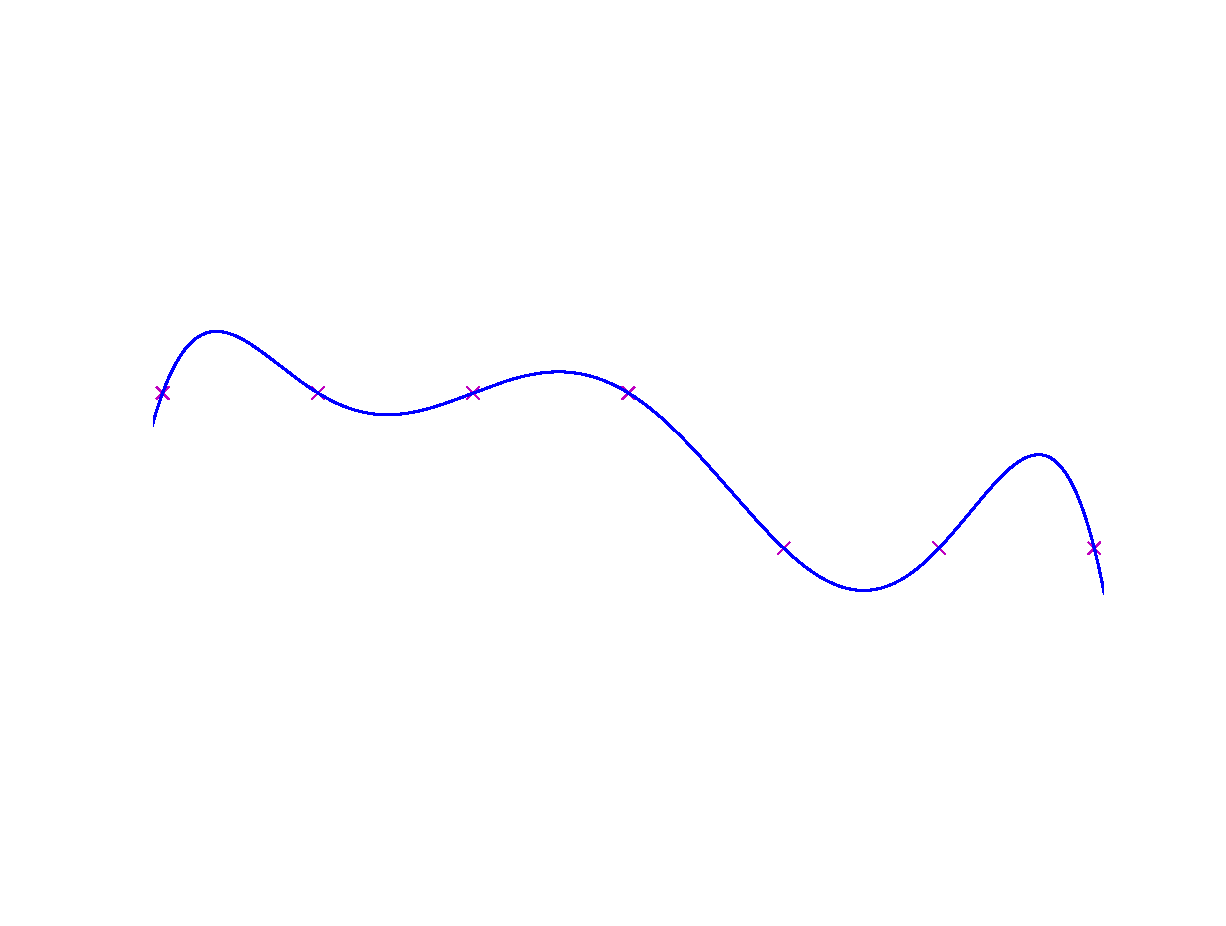
\includegraphics[width=0.45\textwidth]{spline1a}&
\hspace*{-0.5cm}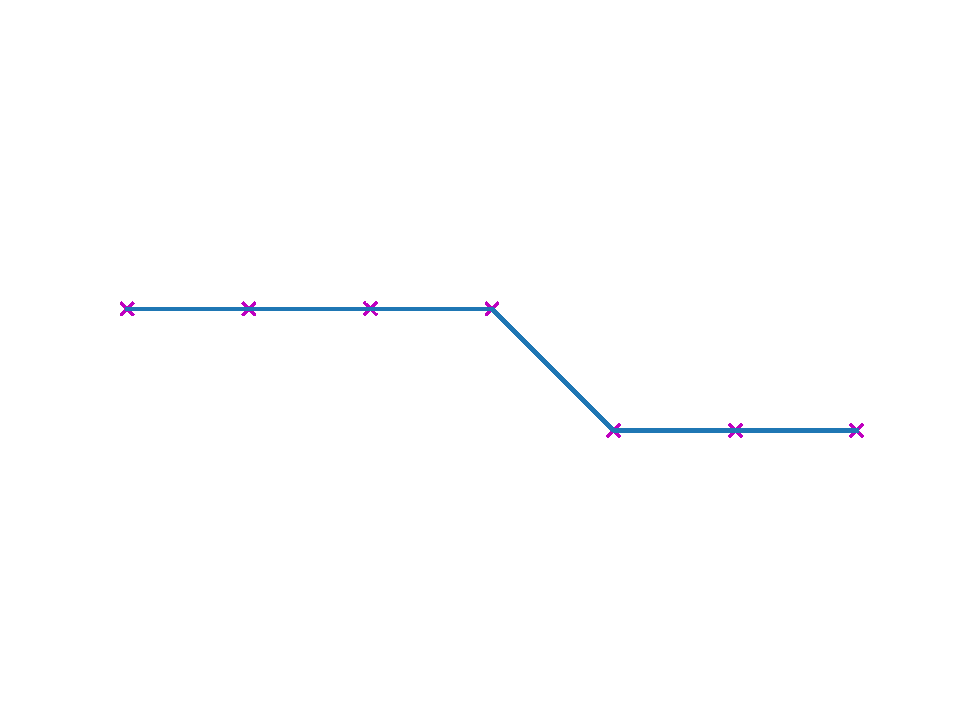
\includegraphics[width=0.45\textwidth]{spline1b}\\
\end{tabular}
\vspace*{-1cm}
\caption{(Piecewise) polynomial approximation of a rough function. Left: the Lagrange interpolant $p_6$ oscillates through the data. Right: the {\bf s}mooth {\bf p}iecewise {\bf line}ar (spline) interpolant, formed via joining consecutive data points, appears to interpolate the data more faithfully.}
\label{figure:SplineIntro}
\end{center}
\end{figure}

Given the theory we have developed for global polynomial approximation via Lagrange interpolating polynomials, it should be clear that there exists a unique solution to the interpolation problem of linear interpolating splines. Furthermore, if we start making regularity assumptions on the data, as if they were samples of a function, then we can demonstrate convergence.

\begin{theorem}\label{theorem:LinearSplineConvergence}
Let $a=x_0<x_1<\cdots<x_n=b$, and let $s(x)$ be the linear interpolating spline. Then, $s\in C([a,b])$ and it is linear on each subinterval $[x_{i-1},x_i]$, for $i=1,\ldots,n$. Let $f(x)\in C^2([a,b])$. Then:
\[
\norm{f-s}_\infty \le \dfrac{h^2}{8}\norm{f''}_\infty,
\]
where $\displaystyle h=\max_{1\le i\le n}(x_i-x_{i-1})$.
\end{theorem}
The nodes $x_i$ for $i=0,\ldots,n$ are known as the {\em knots} of the linear spline.

The linear interpolating spline $s(x)$ can be constructed by calculating slopes of data between knots and using a piecewise definition. Let:
\[
s_i(x) := f(x_{i-1}) + \dfrac{f(x_i)-f(x_{i-1})}{x_i-x_{i-1}}(x-x_{i-1}),\quad{\rm for}\quad i=1,\ldots,n.
\]
Then:
\[
s(x) := \left\{ \begin{array}{ccc}
s_1(x) & \for & x\in[x_0,x_1],\\
\vdots & \vdots & \vdots\\
s_i(x) & \for & x\in[x_{i-1},x_i],\\
\vdots & \vdots & \vdots\\
s_n(x) & \for & x\in[x_{n-1},x_n].\\
\end{array}\right.
\]
Note that we can take either the value of $s_i$ or $s_{i+1}$ at the knot $x_i$ since they are equal.

It may occur that we would like to construct piecewise polynomial interpolants with higher polynomial degree on each subinterval. It is clear that we will want our splines to continue to be interpolatory in nature, thus we will have $2n$ interpolation conditions. With piecewise linear splines, we had $2n$ unknown coefficients and these coefficients are uniquely determined. But if we use piecewise {\em quadratic} splines, then we would have $3n$ unknown coefficients and still only $2n$ interpolation conditions, and generally $(m+1)n$ unknown coefficients with piecewise splines of degree-$m$ and only $2n$ interpolation conditions.

Instead, the added unknowns in piecewise splines of higher degree allow us to enforce continuity of the interpolant, and as many of its higher order derivatives in proportion to the degree. Thus, piecewise quadratics allow for continuity of the first derivative, piecewise cubics allow for continuity of the second derivative, and so on and so forth. These continuity conditions are only applicable at the interior knots $x_1,\ldots,x_{n-1}$, and thus these conditions only give $(m-1)(n-2)$ additional conditions, where $(m-1)$ is the number of derivatives of the spline that are continuous.

Numerous methods have been proposed to add the extra conditions required to ensure that:
\[
\underbrace{(2n)}_{\hbox{interpolation}} + \underbrace{(m-1)(n-2)}_{\hbox{continuity}} + \underbrace{2(m-1)}_{\hbox{extra}} = \underbrace{(m+1)n.}_{\hbox{\# degrees of freedom}}
\]

\begin{example}
Piecewise cubic interpolating splines enforce continuity in the first and second derivatives and require two extra conditions. Three common ways of fulfilling these conditions are:
\begin{enumerate}
\item specify $s'(x_0)=f'(x_0)$ and $s'(x_n) = f'(x_n)$ if derivative information is available;
\item specify $s''(x_0) = 0 = s''(x_n)$, which gives {\em natural} cubic splines; or,
\item enforce continuity of $s'''$ at $x_1$ and $x_n$, which is usually described at the ``not-a-knot'' condition\footnote{This can be reasoned because the continuity of $s'''$ implies that the first two pieces are the same cubic spline on $[x_0,x_2]$, thus $x_1$ is not a knot, and a similar argument for $x_{n-1}$.}.
\end{enumerate}
\end{example}

\begin{comment}
\subsection{B-splines}

In constructing piecewise splines of degree-$m$, one could express the splines in the monomial basis and express the $(m+1)n$ conditions in a sparse\footnote{The system will be sparse because interpolation conditions only involve one piece at a time, and the continuity conditions only involve neighbouring pieces.} linear system of equations. However, using the special {\em basis} splines (B-splines), we find even more structure.

B-splines are themselves natural piecewise polynomials but are only defined {\em locally}, with the following properties:
\[
B_{i,m}(x_i) = 1,\quad{\rm for}\quad i=m/2-1,\ldots,n-m/2+1,
\]
and $B_{i,m}(x)\equiv 0$ for $x\notin(x_{i-m+1},x_{i+m-1})$, and $\deg(B_{i,m}(x)) = m$. The first and last few B-splines have special definitions.

\begin{example}
Construction of the degree-$3$ B-spline with knots $0,1,2,3,4$. On $[0,1]$ we know that:
\[
B_{2,3}(x) = \alpha x^3,
\]
for some $a$ in order that $B_{2,3}$, $B_{2,3}'$, and $B_{2,3}''$ are all continuous at $x=0$. This implies:
\[
B_{2,3}(1) = \alpha,\quad B_{2,3}'(1) = 3\alpha,\quad{\rm and}\quad B_{2,3}''(1) = 6\alpha.
\]
On $[1,2]$, since $B_{2,3}$ is a cubic polynomial, it can be expressed as:
\begin{align*}
B_{2,3}(x) & = B_{2,3}(1) + B_{2,3}'(1)(x-1) + \dfrac{B_{2,3}''(1)}{2}(x-1)^2 + \beta(x-1)^3,\\
& = a + 3a(x-1) + 3a(x-1)^2 + \beta(x-1)^3,
\end{align*}
for some $\beta$. Since we require $B_{2,3}(2) = 1$, then $1 = 7\alpha + \beta$. Now, in order to continue, by symmetry, we must have $B_{2,3}'(2) = 0$, or:
\[
3\alpha+6\alpha + 3\beta = 9\alpha + 3 - 21\alpha = 3-12\alpha = 0,
\]
or $\alpha = \tfrac{1}{4}$ and $\beta = -\tfrac{3}{4}$. Thus:
\[
B_{2,3}(x) = \left\{\begin{array}{ccc}
0 & \for & x<0,\\
\frac{1}{4}x^3 & \for & x\in[0,1],\\
\frac{1}{4} + \frac{3}{4}(x-1) + \frac{3}{4}(x-1)^2 - \frac{3}{4}(x-1)^3 & \for & x\in[1,2],\\
\frac{1}{4} + \frac{3}{4}(3-x) + \frac{3}{4}(3-x)^2 - \frac{3}{4}(3-x)^3 & \for & x\in[2,3],\\
\frac{1}{4}(4-x)^3 & \for & x\in[3,4],\\
0 & \for & x>4.
\end{array}\right.
\]
\end{example}
\end{comment}

\section{Problems}
\begin{enumerate}
\item Na\"ively, one might expect to obtain a formula for the error of the derivative of the Lagrange interpolating polynomial $f'-p_n'$. However, it is not clear that $\xi = \xi(x)$ in Theorem~\ref{theorem:LagrangeInterpolatingRemainder} is even differentiable. An alternative approach leads to the following formula. Prove (and state conditions) that there exist distinct points $z_i\in(x_i,x_{i+1})$ for $i=0,\ldots,n-1$ such that:
\[
\rho_n(x) := f'(x) - p_n'(x) = \dfrac{f^{(n+1)}(\eta)}{n!}\prod_{i=0}^{n-1}(x-z_i),
\]
for some $\eta\in(a,b)$ and for each $x\in[a,b]$. {\em Hint: take the error formula $r(x)$ in Theorem~\ref{theorem:LagrangeInterpolatingRemainder}, and apply the Intermediate Value Theorem on each sub-interval $(x_i,x_{i+1})$ for $i=0,\ldots,n-1$. This gives you the $n$ points $z_i$ where $f'(z_i) - p_n'(z_i) = 0$.}
\item It is sometimes possible to obtain explicit formul\ae~for the barycentric weights $\lambda_k$. Show that for the equispaced nodes in $[-1,1]$, $x_k = -1 + 2k/n$ for $k=0,\ldots,n$, the barycentric weights are:
\[
\lambda_k = \dfrac{(-\tfrac{n}{2})^n}{n!}\binom{n}{k}(-1)^k.
\]
Why may we discard the first part, depending only on $n$, and use the modified weights:
\[
\tilde{\lambda}_k = \binom{n}{k}(-1)^k,
\]
in the second barycentric formula?
\begin{comment}
\item The (symmetrically truncated) cardinal series of a function $f$ is defined by:
\[
C_n(f,h)(x) = \sum_{k=-n}^n f(kh) \sinc\left(\dfrac{x-kh}{h}\right),
\]
where $h>0$ is the spacing of the data and the $\sinc$ function is defined by:
\[
\sinc(x) := \left\{\begin{array}{ccc} \dfrac{\sin(\pi x)}{\pi x}, & \for & x\ne 0,\\ 1, & \for & x = 0.\end{array}\right.
\]
Under appropriate conditions, $C_n(f,h)(x)$ approximates $f(x)$ on $[-nh,nh]$.
\begin{enumerate}
\item Show that:
\[
C_n(f,h)(x) = \dfrac{h}{\pi}\sin\dfrac{\pi x}{h}\sum_{k=-n}^n \dfrac{(-1)^k}{x-kh}f(kh),
\]
or the first barycentric formula for the cardinal series. Since this requires the evaluation of only one value of the sine function, it provides a more efficient way to evaluate the cardinal series that by definition.
\item If instead of approximating $f$ we approximate the weighted function $wf$, where $w>0$, we obtain the modified cardinal series:
\[
C_n(f,h,w)(x) = \dfrac{1}{w(x)}\sum_{k=-n}^n w_kf(kh) \sinc\left(\dfrac{x-kh}{h}\right),
\]
where $w_k = w(kh)$. Under certain conditions on $w$, we may still expect to approximate $f(x)$ on $[-nh,nh]$ by $C_n(f,h,w)(x)$. Use a cardinal series for $w$ to show that:
\[
C_n(f,h,w)(x) \approx \dfrac{\displaystyle\sum_{k=-n}^n \dfrac{(-1)^kw_k}{x-kh}f(kh)}{\displaystyle\sum_{k=-n}^n \dfrac{(-1)^kw_k}{x-kh}}.
\]
This is the second barycentric formula for the cardinal series. It reduces approximation by cardinal series to a rational approximation of $f$.
\item Write a program to approximate $f(x) = \dfrac{1}{1+e^x}$ with a cardinal series on the interval $[-10,10]$ using the weight function $w(x) = e^{-x^2}$.
\end{enumerate}
\end{comment}
\item Generalize Horner's rule for numerical evaluation of polynomials in the monomial basis to numerical evaluation of polynomial interpolants in Newton form.
%\item Under what conditions on the inner product space $L^2(D,w(x)\ud x)$ are even-degree orthogonal polynomials even and odd-degree orthogonal polynomials odd?
\item The Chebyshev expansion of a function $f\in L^2(\I,(1-x^2)^{-\frac{1}{2}}\ud x)$ is determined by:
\[
f(x) \sim \sum_{n=0}^\infty c_n T_n(x),\quad{\rm where}\quad c_n = \dfrac{\langle T_n, f\rangle}{\langle T_n, T_n\rangle}.
\]
In some instances, Chebyshev expansions are known in closed form, such as:
\[
f(x) = \dfrac{1}{x^2+a^2} \sim \dfrac{1}{a\sqrt{a^2+1}}\left(1+2\sum_{n=1}^\infty\dfrac{(-1)^n}{(a+\sqrt{a^2+1})^{2n}}T_{2n}(x)\right),\quad{\rm for}\quad a>0.
\]
\begin{enumerate}
\item Show that:
\[
\langle T_0,T_0\rangle = \pi,\quad{\rm and}\quad \langle T_n,T_n\rangle = \dfrac{\pi}{2},\quad{\rm for}\quad n\in\N.
\]
\item Calculate $\norm{f}_{\infty}$ and $\norm{f}_{2,w}$, the weighted $2$-norm associated with $L^2(\I,(1-x^2)^{-\frac{1}{2}}\ud x)$. {\em Hint: for the weighted $2$-norm, use the Chebyshev expansion and orthogonality of the Chebyshev polynomials.}
\item Let $p_N(x)$ denote the degree-$N$ Chebyshev expansion of $f$.
Which $N( = N(a,\varepsilon))$ is required to satisfy:
\[
\norm{f-p_N}_{2,w} \le \varepsilon\norm{f}_{2,w}?
\]
\item Which $N( = N(a,\varepsilon))$ is required to satisfy:
\[
\norm{f-p_N}_\infty \le \varepsilon\norm{f}_\infty?
\]
\end{enumerate}

\item Calculate the first five orthogonal polynomials with respect to $L^2([-1,-a]\cup[a,1],\ud x)$ for some $a\in[0,1)$. While inapplicable, Theorem~\ref{theorem:OPzeros} makes a statement on the locii of the zeros of orthogonal polynomials with respect to $L^2([a,b],\ud\mu(x))$ for some monotonic measure $\mu$. Can anything be said about the locii of the zeros in the current case? What do you expect when $\lim_{a\to0}\pi_n(x;a)$?
\item Prove Theorem~\ref{theorem:LinearSplineConvergence}.
\end{enumerate}
% !TEX root = ./MATH2160.tex
\chapter{Numerical Differentiation and Integration}\label{chapter:Calculus}

Given a differentiable function, we can always find its derivative, although this may not be inviting if the function is complicated. Numerical differentiation approximates the derivative using only function values. Numerical differentiation formul\ae~can be used for solving initial-value problems and other differential equations. Integration is another problem that can be handled numerically only using function values. Numerical integration is clearly useful since there are many functions that cannot be integrated by hand nor analytically by powerful symbolic software, and often the analytical expressions that {\em do} exist are numerically impractical.

\section{Finite Differences}

Given $f\in C^1((a,b))$, recall that:
\[
f'(x) = \lim_{h\to0}\dfrac{f(x+h)-f(x)}{h}.
\]
For a sufficiently small $h$, we can make the approximation:
\[
f'(x) \approx \dfrac{f(x+h)-f(x)}{h}.
\]
Let us study the error in this approximation, which is known as the {\bf first-order forward difference}. From Taylor's remainder theorem, if we assume $f\in C^2((a,b))$:
\[
\left|f'(x) - \dfrac{f(x+h)-f(x)}{h}\right| \le \dfrac{h}{2}\max_{\xi\in(a,b)}|f''(\xi)|.
\]
Since this error term holds for all $x\in(a,b)$, we say that this approximation is of first-order. If we take a small step backward instead, then we arrive at the backward difference formula:
\[
f'(x) \approx \dfrac{f(x)-f(x-h)}{h},
\]
which has the same upper bound on the error as the forward difference.

In many applications, this is not accurate enough. Higher order schemes can be created by ensuring more terms in the Taylor series are removed as $h\to0$ in the formula. Consider the second-order formula created by averaging the forward and backward differences:
\[
f'(x) \approx \dfrac{f(x+h)-f(x-h)}{2h}.
\]
This is called a centered difference scheme. To see this, subtract the Taylor expansions:
\[
f(x\pm h) = f(x) \pm f'(x)h + \dfrac{f''(x)}{2}h^2 \pm \dfrac{f'''(c_\pm)}{6}h^3,
\]
for some constants $c_\pm\in(x,x\pm h)$ to obtain:
\[
\left|f'(x) - \dfrac{f(x+h)-f(x-h)}{2h}\right| = \left|\dfrac{f'''(c_+) + f'''(c_-)}{12}h^2\right| \le \dfrac{h^2}{6}\max_{\xi\in(a,b)}|f'''(\xi)|,
\]
for all $x\in(a,b)$.

It is not difficult to derive a second-order finite difference approximation of the second derivative. Assume that $f\in C^4((a,b))$. Adding the Taylor expansions:
\[
f(x\pm h) = f(x) \pm f'(x)h + \dfrac{f''(x)}{2}h^2 \pm \dfrac{f'''(x)}{6}h^3 + \dfrac{f^{({\rm iv})}(c_\pm)}{24}h^4,
\]
we obtain, after some algebra:
\[
f''(x) \approx \dfrac{f(x+h)-2f(x) + f(x-h)}{h^2},
\]
and indeed the approximation is second-order since:
\[
\left|f''(x) - \dfrac{f(x+h)-2f(x) + f(x-h)}{h^2}\right| = \left|\dfrac{f^{({\rm iv})}(c_+) + f^{({\rm iv})}(c_-)}{24}h^2\right| \le \dfrac{h^2}{12}\max_{\xi\in(a,b)}|f^{({\rm iv})}(\xi)|.
\]

\subsection{Complex Differences}

Consider using the Taylor expansion of $f$ with a small perturbation into the complex plane:
\[
f(x+\i h) = f(x) + \i f'(x)h - \dfrac{f''(x)}{2}h^2 - \i\dfrac{f'''(c)}{6}h^3,
\]
where $c-x\in\i(0,h)$. This expansion motivates the complex finite difference formula:
\[
f'(x) \approx \Im\left\{\dfrac{f(x+\i h)}{h}\right\},
\]
which is second-order since:
\[
\left|f'(x) - \Im\left\{\dfrac{f(x+\i h)}{h}\right\}\right| = \left|\dfrac{f'''(c)}{6}h^2\right| \le \dfrac{h^2}{6}\max_{\xi\in(x,x+\i h)}|f'''(\xi)|.
\]
Using just a single function evaluation in the complex difference formula, we obtain second-order accuracy equivalent to the centered difference formula! Furthermore, as there is no subtraction involved in the complex finite difference formula, we expect the formula to have better numerical stability properties. Indeed, Figure~\ref{figure:FiniteDifferences} shows the resulting error when numerically differentiating $f(x) = e^x$ at $x=1$ using the first- and second-order finite difference formul\ae~and the second-order complex finite difference formula.

\begin{figure}[htbp]
\begin{center}
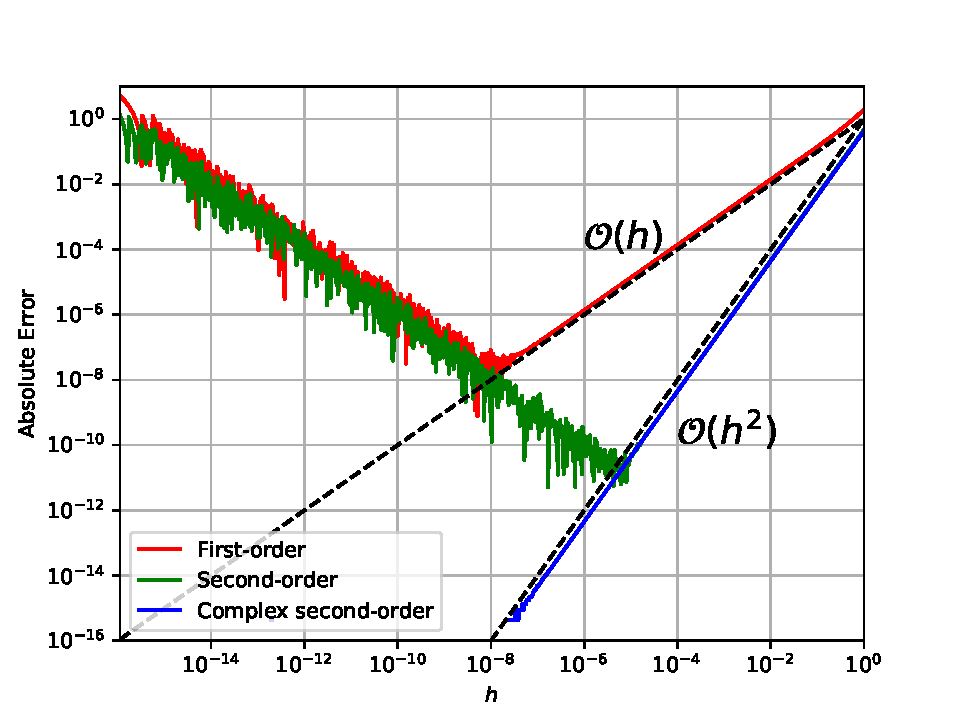
\includegraphics[width=0.65\textwidth]{finitedifferences}
\caption{Comparison of first- and second-order finite difference formul\ae~and the second-order complex finite difference formula for $f(x)=e^x$ at $x=1$. The dashed black lines are representative first- and second-order scalings.}
\label{figure:FiniteDifferences}
\end{center}
\end{figure}

While the complex finite difference formul\ae~are impressive, and relieve the numerical instability of finite difference formul\ae~due to subtractive cancellation, the ability to numerically evaluate a function in the complex plane assumes {\em analyticity}, which is much stronger than the weak assumptions of second- and third-order differentiability. So, any comparison with complex finite differencing is unfair.

\subsection{Dual Numbers and Forward-Mode Automatic Differentiation}

Let $\F$ be the field of real or complex numbers $\R$ or $\C$. Dual numbers extend the field $\F$ with a unit dual $\varepsilon$ to the quotient ring $\D:= \F[\varepsilon]/(\varepsilon^2)$, i.e. the unit dual number satisfies $\varepsilon^2=0$. Thus, it is clear that dual numbers obey the following rules for addition and multiplication:
\[
(a+b\varepsilon) + (c+d\varepsilon) = (a+c) + (b+d)\varepsilon,\quad{\rm and}\quad (a+b\varepsilon)(c+d\varepsilon) = ac + (ad+bc)\varepsilon.
\]
Remarkably, the product of two dual numbers is the product of the two primal components and the dual component can be interpreted as the product rule differentiation formula.
\begin{example}
Let $f(x) = x^2$. Then evaluation at the dual number $x=a+b\varepsilon$ is:
\[
f(a+b\varepsilon) = (a+b\varepsilon)^2 = a^2 + 2ab\varepsilon.
\]
\end{example}
Dual numbers can be interpreted as evaluation at the matrix:
\[
\begin{bmatrix}
a & b\\
0 & a\\
\end{bmatrix},
\]
since this matrix satisfies the addition and multiplication rules of $\D$.
\begin{example}
Let $f(x) = e^x$. The evaluation at the dual number $x=a+b\varepsilon$ can be achieved via the matrix exponential. Since $A:=\diag(a,a)$ and $B:=\begin{bmatrix} 0 & b\\0 & 0\\\end{bmatrix}$ commute, i.e. $AB=BA$, using the property $e^{A+B} = e^Ae^B$, we find:
\[
e^{a+b\varepsilon} = e^{A+B} = e^Ae^B = \begin{bmatrix}e^a & 0\\ 0 & e^a\\\end{bmatrix}\begin{bmatrix}1 & b\\ 0 & 1\\\end{bmatrix} = \begin{bmatrix}e^a & be^a\\ 0 & e^a\\\end{bmatrix} = e^a(1+b\varepsilon).
\]
\end{example}

These simple examples motivate the following definition for evaluation of a function at a dual number.
\begin{definition}
Let $D\subset\F$. Evaluation of $f$ at a dual number $x\in D$ is defined by:
\begin{equation}
f(a+b\varepsilon) := f(a) + \lim_{h\to0}\dfrac{f(a+b\varepsilon h)-f(a)}{h}.
\end{equation}
\end{definition}
When $f$ is differentiable at $a$, we can identify the limit as the derivative:
\[
f(a+b\varepsilon) = f(a) + f'(a)b\varepsilon.
\]

Endowed with only the above properties, dual numbers are a powerful tool for numerical differentiation. In fact, the dual component of the differentiable function $f(a+b\varepsilon)$ {\em is} the function's derivative scaled by $b$, effectively implementing the chain rule differentiation formula since $b$ is allowed to store other differentiation information. Since multiplication of two dual numbers implements the product rule differentiation formula, we have everything we need in order to evaluate complicated derivatives on a computer. In any computer programming language that allows {\em operator overloading}, we can {\em overload} the functions 
\begin{verbatim}
exp(x::Dual) = exp(x.value) * (1 + x.dual * epsilon)
sin(x::Dual) = sin(x.value) + x.dual * cos(x.value) * epsilon
cos(x::Dual) = cos(x.value) - x.dual * sin(x.value) * epsilon
\end{verbatim}
In this pseudocode, the double colon indicates a type assertion, i.e. \verb+x+ must be a number of the type \verb+Dual+, the dot following the variable \verb+x+ accesses the field storing the primal entry \verb+value+ or the dual entry \verb+dual+, and \verb+epsilon+ is used to indicate the unit dual number $\varepsilon$.

Any function that we create from this point onward that uses \verb+exp+, \verb+sin+, or \verb+cos+, can return the derivative in the dual component.

\begin{example}
Evaluate the derivative of $f(x) = e^{\sin x} + \cos(\sin(e^x))$ at the point $x=1$. Using the rules outlined above, we evaluate $f$ at the dual number $x = 1 + \varepsilon$, and obtain:
\[
f(1+\varepsilon) = 3.236585937969746 + 2.243049618601819\varepsilon,
\]
which turns out to be a correctly rounded result in 64-bit floating-point arithmetic.
\end{example}

This use of dual numbers is known as forward-mode automatic differentiation, and is extremely important in optimization problems, where large Jacobian vectors and Hessian matrices are required.

\section{Newton--Cotes Quadrature}

In this section and beyond, the word quadrature can be taken to mean numerical integration.
\begin{definition}
Any formula of the form:
\[
\int_a^b f(x)\ud x \approx \sum_{k=0}^n w_k f(x_k),
\]
where the nodes $x_k\in[a,b]$ and the weights $w_k$ are independent of $f$ is called a {\bf quadrature formula}.
\end{definition}
We have seen that under certain conditions the Lagrange interpolating polynomials can do quite well in approximating a function $f$. Given the $n+1$ equispaced points $x_k = x_0+kh$, for $k=0,\ldots,n$, and where $h=(x_n-x_0)/n$, if $p_n(x_k) = f(x_k)$, how good of an approximation is:
\begin{equation}\label{eq:NewtonCotes}
\int_{x_0}^{x_n} f(x)\ud x \approx \int_{x_0}^{x_n} p_n(x)\ud x ?
\end{equation}
Note that the right-hand side of~\eqref{eq:NewtonCotes} can be expressed using the Lagrange basis polynomials:
\begin{align}
\int_{x_0}^{x_n} p_n(x)\ud x & = \int_{x_0}^{x_n} \sum_{k=0}^n f(x_k) \ell_{n,k}(x)\ud x,\nonumber\\
& = \sum_{k=0}^n f(x_k) \int_{x_0}^{x_n} \ell_{n,k}(x)\ud x,\\
& = \sum_{k=0}^n w_k f(x_k),\nonumber
\end{align}
where the weights:
\begin{equation}\label{eq:NewtonCotesWeights}
w_k := \int_{x_0}^{x_n} \ell_{n,k}(x)\ud x,\quad{\rm for}\quad k=0,\ldots,n,
\end{equation}
are independent of $f$. The specific form~\eqref{eq:NewtonCotes}--\eqref{eq:NewtonCotesWeights} of quadrature formul\ae~based on equispaced points are called the {\bf Newton--Cotes} family of quadrature formul\ae.

Classical examples of the Newton--Cotes family are the:
\begin{description}
\item[Trapezoidal Rule] where the formula:
\[
\int_{x_0}^{x_1}f(x)\ud x \approx \dfrac{h}{2}\br[f(x_0)+f(x_1)],
\]
follows from:
\begin{align*}
\int_{x_0}^{x_1}p_1(x)\ud x & = f(x_0)\int_{x_0}^{x_1}\overbrace{\dfrac{x-x_1}{x_0-x_1}}^{\ell_{1,0}(x)}\ud x + f(x_1)\int_{x_0}^{x_1}\overbrace{\dfrac{x-x_0}{x_1-x_0}}^{\ell_{1,1}(x)}\ud x,\\
& = f(x_0)\dfrac{(x_1-x_0)}{2} + f(x_1)\dfrac{(x_1-x_0)}{2};\hbox{ and},
\end{align*}
\item[Simpson's Rule] with the formula:
\[
\int_{x_0}^{x_2}f(x)\ud x \approx \dfrac{h}{3}\br[f(x_0)+4f(x_1)+f(x_2)].
\]
\end{description}

Using Theorem~\ref{theorem:LagrangeInterpolatingRemainder} characterizing the remainder in the Lagrange interpolating polynomial, we can immediately derive the remainder for the Newton--Cotes family.
\begin{theorem}\label{theorem:NewtonCotesLIRError}
Suppose that $f\in C^{n+1}((x_0,x_n))$. The remainder in the Newton--Cotes family of quadrature formul\ae~is given by:
\begin{equation}
\int_{x_0}^{x_n}[f(x)-p_n(x)]\ud x = \int_{x_0}^{x_n} \dfrac{\ell(x)}{(n+1)!}f^{(n+1)}(\xi(x))\ud x.
\end{equation}
\end{theorem}
Taking the absolute value, we can bound the error by:
\[
\left|\int_{x_0}^{x_n}[f(x)-p_n(x)]\ud x\right| \le \dfrac{1}{(n+1)!}\max_{\xi\in(x_0,x_n)}|f^{(n+1)}(\xi)|\int_{x_0}^{x_n} |\ell(x)|\ud x,
\]
which, for the trapezoidal rule gives:
\[
\left|\int_{x_0}^{x_n}f(x)\ud x - \dfrac{h}{2}\br[f(x_0)+f(x_1)]\right| \le \dfrac{(x_1-x_0)^3}{12}\max_{\xi\in(x_0,x_n)}|f''(\xi)|.
\]
In fact, we can prove tighter results using the Integral Mean Value Theorem.
\begin{theorem}\label{theorem:TrapezoidalIMVTError}
Suppose $f\in C^2((x_0,x_1))$. Then:
\[
\int_{x_0}^{x_1}f(x)\ud x - \dfrac{h}{2}\br[f(x_0)+f(x_1)] = -\dfrac{(x_1-x_0)^3}{12}f''(\xi),\quad\hbox{for some}\quad \xi\in(x_0,x_1).
\]
\end{theorem}

For $n>1$, the bounds generated by Theorem~\ref{theorem:NewtonCotesLIRError} are even more pessimistic. In fact, one can prove better results such as:
\begin{theorem}
Suppose $f\in C^4((x_0,x_2))$. Then:
\[
\left|\int_{x_0}^{x_2}f(x)\ud x - \dfrac{h}{3}\br[f(x_0)+4f(x_1)+f(x_2)]\right| \le \dfrac{(x_2-x_0)^5}{720}\max_{\xi\in(x_0,x_2)}|f^{({\rm iv})}(\xi)|.
\]
\end{theorem}
\begin{proof}
Since $h = (x_2-x_0)/2 = x_1-x_0 = x_2-x_1$, consider the difference $f(x_0) -2f(x_1)+f(x_2) = f(x_1-h)-2f(x_1)+f(x_1+h)$. Using the Taylor expansions:
\begin{align*}
f(x_1-h) & \quad f(x_1) - hf'(x_1) + \tfrac{1}{2}h^2f''(x_1) - \tfrac{1}{6}h^3f'''(x_1) + \tfrac{1}{24}h^4f^{({\rm iv})}(\xi_1)\\
-2f(x_1) & = -2f(x_1) +\\
+f(x_1+h) & \quad f(x_1) + hf'(x_1) + \tfrac{1}{2}h^2f''(x_1) + \tfrac{1}{6}h^3f'''(x_1) + \tfrac{1}{24}h^4f^{({\rm iv})}(\xi_2),
\end{align*}
for some $\xi_1\in(x_0,x_1)$ and $\xi_2\in(x_1,x_2)$, and hence:
\begin{equation}\label{eq:SimpsonsSecondDifference}
f(x_0)-2f(x_1)+f(x_2) = h^2f''(x_1) + \tfrac{1}{24}h^4\br[f^{({\rm iv})}(\xi_1) + f^{({\rm iv})}(\xi_2)] = h^2f''(x_1) + \tfrac{1}{12}h^4f^{({\rm iv})}(\xi_3),
\end{equation}
for some $\xi_3\in(\xi_1,\xi_2)\subset(x_0,x_2)$, due to the Intermediate Value Theorem. Now, for any $x\in[x_0,x_2]$, we again use Taylor expansions to deduce:
\begin{align*}
\int_{x_0}^{x_2}f(x)\ud x & = f(x_1)\int_{x_1-h}^{x_1+h}\ud x + f'(x_1)\int_{x_1-h}^{x_1+h}(x-x_1)\ud x\\
& ~~ + \tfrac{1}{2}f''(x_1)\int_{x_1-h}^{x_1+h}(x-x_1)^2\ud x + \tfrac{1}{6}f'''(x_1)\int_{x_1-h}^{x_1+h}(x-x_1)^3\ud x\\
& ~~ + \tfrac{1}{24}\int_{x_1-h}^{x_1+h} f^{({\rm iv})}(\eta_1(x))(x-x_1)^4\ud x\\
& = 2hf(x_1) + \tfrac{1}{3}h^3f''(x_1) + \tfrac{1}{60}h^5f^{({\rm iv})}(\eta_2)\\
& = \tfrac{h}{3}\br[f(x_0)+4f(x_1)+f(x_2)] + \tfrac{1}{60}h^5f^{({\rm iv})}(\eta_2) - \tfrac{1}{36}h^5f^{({\rm iv})}(\xi_3),\\
& = \int_{x_0}^{x_2}p_2(x)\ud x + \dfrac{1}{180}\left(\dfrac{x_2-x_0}{2}\right)^5(3f^{({\rm iv})}(\eta_2) - 5f^{({\rm iv})}(\xi_3)),
\end{align*}
where $\eta_1(x),\eta_2\in(x_0,x_2)$, and where we have used the Integral Mean Value Theorem and~\eqref{eq:SimpsonsSecondDifference}. Thus, taking moduli, we have:
\[
\left|\int_{x_0}^{x_2}\br[f(x)-p_2(x)]\ud x\right| \le \dfrac{8}{2^5\cdot180}(x_2-x_0)^5\max_{\xi\in(x_0,x_2)}|f^{({\rm iv})}(\xi)|.
\]
\end{proof}

In fact, it is possible to compute a slightly stronger bound.
\begin{theorem}[Theorem 7.2 in S\"uli and Mayers~\cite{Suli-Mayers-03}]
Suppose $f\in C^4((x_0,x_2))$. Then:
\[
\int_{x_0}^{x_2}f(x)\ud x - \dfrac{h}{3}\br[f(x_0)+4f(x_1)+f(x_2)] = -\dfrac{(x_2-x_0)^5}{2880}f^{({\rm iv})}(\xi),
\]
for some $\xi\in(x_0,x_2)$.
\end{theorem}

\begin{remark}
The $n$-point Newton--Cotes formul\ae~are exact if $f\in\P_n$ since $f\in\P_n\Longrightarrow p_n \equiv f$. However, in certain cases, such as Simpson's rule, the degree of exactness is even higher: indeed, if $f\in\P_3$, then $f^{({\rm iv})}\equiv0$ and the formula is exact.
\end{remark}

\subsection{Composite Formul\ae}

In polynomial interpolation, we have seen oscillations and instability set in when approximating high-degree polynomials. One simple fix was to use splines. In direct analogy, for numerical integration we can split an integration interval $[a,b] = [x_0,x_n]$ into $n$ equal subintervals $[x_{i-1},x_i]$ for $i=1,\ldots,n$. Then, we can use a {\bf composite rule}:
\[
\int_a^bf(x)\ud x = \int_{x_0}^{x_n}f(x)\ud x = \sum_{i=1}^n\int_{x_{i-1}}^{x_i}f(x)\ud x,
\]
in which integration through each subinterval is approximated by quadrature. Thus, rather than increase the degree of the polynomials to attain high accuracy, we can increase the number of subintervals.

The first two composite rules are the:
\begin{description}
\item[Composite Trapezoidal Rule] where the formula:
\begin{align*}
\int_{x_0}^{x_n} f(x)\ud x & = \sum_{i=1}^n\left[\dfrac{h}{2}\br[f(x_{i-1})+f(x_i)] - \dfrac{h^3}{12}f''(\xi_i)\right],\\
& = \dfrac{h}{2}\br[f(x_0)+2f(x_1)+\cdots+2f(x_{n-1})+f(x_n)] + e_h^{\rm T},
\end{align*}
where $\xi_i\in(x_{i-1},x_i)$, $h=x_i-x_{i-1} = (x_n-x_0)/n = (b-a)/n$, and the error $e_h^{\rm T}$ is given by:
\[
e_h^{\rm T} = -\dfrac{h^3}{12}\sum_{i=1}^n f''(\xi_i) = -\dfrac{nh^3}{12}f''(\xi) = -(b-a)\dfrac{h^2}{12}f''(\xi),
\]
for some $\xi\in(a,b)$, using the Intermediate Value Theorem $n-1$ times.
\item[Composite Simpson's Rule] where the formula:
\begin{align*}
\int_{x_0}^{x_n} f(x)\ud x & = \sum_{i=1}^{n/2}\left[\dfrac{h}{3}\br[f(x_{2i-2})+4f(x_{2i-1})+f(x_{2i})] - \dfrac{(2h)^5}{2880}f^{({\rm iv})}(\xi_i)\right],\\
& = \dfrac{h}{3}\br[f(x_0)+4f(x_1)+2f(x_2)+\cdots+2f(x_{n-2})+4f(x_{n-1})+f(x_n)] + e_h^{\rm S},
\end{align*}
where $\xi_i\in(x_{2i-2},x_{2i})$, $n$ is an even integer, $h = x_{2i}-x_{2i-1} = (x_n-x_0)/n = (b-a)/n$, and the error $e_h^{\rm S}$ is given by:
\[
e_h^{\rm S} = -\dfrac{(2h)^5}{2880}\sum_{i=1}^{n/2} f^{({\rm iv})}(\xi_i) = -\dfrac{n/2(2h)^5}{2880}f^{({\rm iv})}(\xi) = -(b-a)\dfrac{h^4}{180}f^{({\rm iv})}(\xi),
\]
for some $\xi\in(a,b)$, using the Intermediate Value Theorem $n/2-1$ times.
\end{description}

Figure~\ref{figure:CompositeNewtonCotes} shows the resulting error when numerically integrating $f(x) = e^x$ on $\I$ using the composite trapezoidal and Simpson's rules.

\begin{figure}[htbp]
\begin{center}
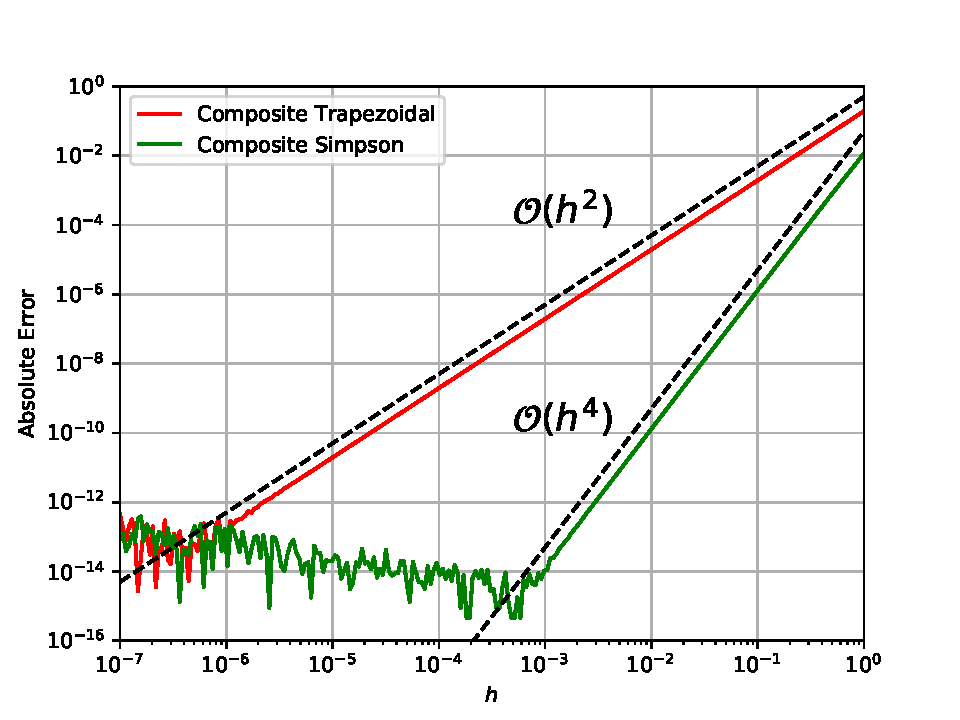
\includegraphics[width=0.65\textwidth]{compositenewtoncotes}
\caption{Comparison of the composite trapezoidal and Simpson's rules for $\int_{-1}^1e^x\ud x$. The dashed black lines are representative second- and fourth-order scalings.}
\label{figure:CompositeNewtonCotes}
\end{center}
\end{figure}

%\subsection{Adaptive Quadrature}
%\subsection{Euler--Maclaurin Summation Formula}

\section{Richardson Extrapolation}

Richardson extrapolation~\cite{Richardson-210-459-11} is an algorithm designed to transform, in certain cases, the asymptotic expansion of the error in a formula into a systematic method that exploits structure of the asymptotic expansion in order to provide a more accurate result. The result is known as an {\em extrapolant} as it is usually beyond reach. Suppose we are interested in the quantity $A$ and we can approximate it by $A_h$, where $h>0$ is some tuneable parameter. Furthermore, suppose we are aware of the asymptotic expansion:
\[
A_h = A + c_1h + c_2h^2 + \cdots + c_nh^n + \OO(h^{n+1}),\quad{\rm as}\quad h\to0.
\]
Such an expansion is motivated by Taylor's theorem, and as such Richardson extrapolation can improve the approximation of derivatives by finite differences and the approximation of integrals by Newton--Cotes quadrature. The next step is to assume we are in the r\'egime where $h$ is truly small, such that we only incur a small error in setting:
\begin{equation}\label{eq:RichardsonExtrapolation}
\hat{A} + \hat{c}_1h + \hat{c}_2h^2 + \cdots + \hat{c}_nh^n = A_h.
\end{equation}
To solve for the $n$ unknowns $\hat{A}$ and $\hat{c}_k$ for $k=1,\ldots,n$, we use $n+1$ distinct values of $h$ to setup and solve the linear system:
\begin{equation}\label{eq:Vandermonde}
\begin{bmatrix}
1 & h_0 & \cdots & h_0^n\\
1 & h_1 & \cdots & h_1^n\\
\vdots & \vdots & \ddots & \vdots\\
1 & h_n & \cdots & h_n^n\\
\end{bmatrix}
\begin{bmatrix} \hat{A}\\\hat{c}_1\\\vdots\\\hat{c}_n\end{bmatrix}
=
\begin{bmatrix} A_{h_0}\\A_{h_1}\\\vdots\\A_{h_n}\end{bmatrix}.
\end{equation}
The matrix in~\eqref{eq:Vandermonde} is known as the Vandermonde matrix. While a direct method would require $\OO(n^3)$ flops for the solution of the unknowns $\hat{A}$ and $\hat{c}_k$, recall that we are only interested in the extrapolant $\hat{A}$: the unknowns $\hat{c}_k$ are auxiliary variables introduced to satisfy the asymptotic expansion. Thus, we may intuitively expect to only require $\OO(n^2)$ operations to only solve for the unknown $\hat{A}$.

We turn to an already familiar tool for the solution. First, we rewrite~\eqref{eq:RichardsonExtrapolation} as follows:
\[
\hat{c}_1 + \hat{c}_2h + \cdots + \hat{c}_nh^{n-1} = \dfrac{A_h-\hat{A}}{h}.
\]
Since the left-hand side is a degree-$(n-1)$ polynomial in $h$, the $n^{\rm th}$ Newton divided difference will annihilate it:
\[
0 \equiv \delta^{(n)}[h_0,\ldots,h_n]\pr(\hat{c}_1 + \hat{c}_2h + \cdots + \hat{c}_nh^{n-1}) = \delta^{(n)}[h_0,\ldots,h_n]\pr(\dfrac{A_h-\hat{A}}{h}).
\]
Since the unknown $\hat{A}$ is a constant (in terms of the parameter $h$), we may isolate for it as follows:
\[
\hat{A} = \dfrac{\displaystyle\delta^{(n)}[h_0,\ldots,h_n]\pr(\frac{A_h}{h})}{\displaystyle\delta^{(n)}[h_0,\ldots,h_n]\pr(\frac{1}{h})}.
\]
Since Newton divided differences can be computed in $\OO(n^2)$ by organizing the calculation in a tableau, we now have a fast method for computing Richardson extrapolants.

\begin{example}
Let us approximate $\pi$ by inscribed polygons in the unit circle. For a regular $n$-gon, the circumference is $2n\sin(\pi/n) \le 2\pi$, so let $C_n = n\sin(\pi/n) \le \pi$ be half the circumference. Indeed, $C_2 = 2\sin(\pi/2) = 2$. Furthermore, we can compute a sequence of circumferences recursively:
\begin{align*}
C_{2n} = 2n\sin(\pi/2n) & = 2n\sqrt{\frac{1}{2}(1-\cos(\pi/n))},\\
& = 2n\sqrt{\frac{1}{2}\left(1-\sqrt{1-\sin^2(\pi/n)}\right)},\\
& = 2n\sqrt{\frac{1}{2}\left(1-\sqrt{1-(C_n/n)^2}\right)}.
\end{align*}
Since this expression is sensitive to rounding errors, we rewrite it as:
\[
C_{2n} = \dfrac{C_n\sqrt{2}}{\sqrt{1+\sqrt{1-(C_n/n)^2}}}.
\]
If we let $h = 1/n^2$, then:
\[
C_{1/\sqrt{h}} = A_h = \dfrac{\sin(\pi \sqrt{h})}{\sqrt{h}} = \pi - \dfrac{\pi^3h}{6} + \dfrac{\pi^5h^2}{120}+\cdots+.
\]

Table~\ref{table:Richardson1} shows the result of applying Richardson extrapolation when $h = 1/n^2$ for $n=2,4,8,\ldots.$ Bold digits represent correct values when approximating $\pi$.
\begin{table}[htdp]
\caption{Richardson extrapolation of the circumference of an $n$-gon.}
\begin{center}
\begin{tabular}{rll}
\hline
$n$ & $C_n$ & Richardson Extrapolants\\
\hline
$2$ & $2.000000000000000$ & $2.000000000000000$\\
$4$ & $2.8284271247461903$ & ${\bf 3.1}04569499661587$\\
$8$ & ${\bf 3}.0614674589207187$ & ${\bf 3.141}4527750222714$\\
$16$ & ${\bf 3.1}21445152258053$ & ${\bf 3.141592}5775443454$\\
$32$ & ${\bf 3.1}365484905459398$ & ${\bf 3.14159265358}3072$\\
$64$ & ${\bf 3.14}0331156954754$ & ${\bf 3.14159265358979}44$\\
$128$ & ${\bf 3.141}277250932774$ & ${\bf 3.14159265358979}5$\\
$256$ & ${\bf 3.1415}138011443027$ & ${\bf 3.14159265358979}5$\\
\hline
$+\infty$ & ${\bf 3.141592653589793\cdots}$ & ${\bf 3.141592653589793\cdots} =\pi$\\
\hline
\end{tabular}
\end{center}
\label{table:Richardson1}
\end{table}%
\end{example}

\section{Gaussian Quadrature}

While the family of (composite) Newton--Cotes quadrature formul\ae~take equispaced nodes, if we relax this restriction, then the resulting quadrature formula can be more accurate. Consider the problem of choosing the nodes and weights in the quadrature formula:
\[
\int_a^bf(x)w(x)\ud x \approx \sum_{k=1}^n w_kf(x_k)
\]
so that the rule is exact for polynomials of degree as high as possible. Being optimistic, with $n$ nodes and weights at our disposal, we hope it will satisfy $2n$ exactness conditions of the type:
\[
\int_a^b x^m w(x)\ud x = \sum_{k=1}^n w_k x_k^m,\quad{\rm for}\quad m=0,\ldots,2n-1.
\]
The word ``hope'' was used in the previous sentence because these last equations, while linear in the weights, are nonlinear in the nodes. Hence, these might {\em a priori} be complex numbers or even real numbers outside of $(a,b)$. In either case, the quadrature formula would be useless. Fortunately, the following theorem relates the nodes of the Gaussian quadrature formula to the zeros of the orthogonal polynomials, and by construction, it follows that these nodes are located within the interval $(a,b)$.

\begin{theorem}\label{theorem:Gaussnodesandweights}
Let $w\ge0$ be a non-negative weight function on $[a,b]$ and let $a,b,\in\R$. Then:
\begin{enumerate}
\item the nodes of the Gaussian quadrature formula are the zeros of the orthogonal polynomial $\pi_n$ with respect to $L^2([a,b],w(x)\ud x)$;
\item The formula:
\[
\int_a^bf(x)w(x)\ud x = \sum_{k=1}^n w_kf(x_k),
\]
is exact for every $f\in\P_{2n-1}$; and,
\item The weights $w_k>0$ for $k=1,\ldots,n$.
\end{enumerate}
\end{theorem}
\begin{proof}
Let $\pi_n$ be the degree-$n$ orthogonal polynomial with respect to $L^2([a,b],w(x)\ud x)$, and let $x_1,\ldots,x_n$ be its zeros. If $f\in\P_{2n-1}$, there exists $q,r\in\P_{n-1}$ such that $f = q\pi_n + r$. Since $x_k$ are the roots of $\pi_n$, it follows that $f(x_k) = r(x_k)$ for $k=1,\ldots,n$. Hence:
\[
r(x) = \sum_{k=1}^n \ell_{n,k}(x) f(x_k),
\]
where $\ell_{n,k}(x)\in\P_{n-1}$ for $k=1,\ldots,n$ are the Lagrange basis polynomials through the roots of $\pi_n$. We integrate to obtain:
\begin{align*}
\int_a^b f(x)w(x)\ud x & = \int_a^b\left(q(x)\pi_n(x)+r(x)\right)w(x)\ud x,\\
& = \int_a^b q(x)\pi_n(x)w(x)\ud x + \int_a^br(x) w(x)\ud x,\\
& = 0 + \sum_{k=1}^nw_kf(x_k),
\end{align*}
where the $q\pi_n$ integrates to $0$ by orthogonality and where:
\[
w_k = \int_a^b \ell_{n,k}(x)w(x)\ud x,\quad{\rm for}\quad k=1,\ldots,n.
\]
Clearly, 1.~holds by applying Theorem~\ref{theorem:OPzeros}, 2.~holds without loss of generality, and 3.~holds by repeating the argument with the alternative interpolant:
\[
f(x) = q(x)\pi_n(x) + \sum_{k=1}^n\left[\ell_{n,k}(x)-\ell_{n,k}^2(x)\right]f(x_k) + \sum_{k=1}^n\ell_{n,k}^2(x)f(x_k),\in\P_{2n-1},
\]
and since $\ell_{n,k}-\ell_{n,k}^2$ is zero at each of the roots, $\pi_n$ is a divisor.
\end{proof}

\begin{remark}
Note that due to the limiting form of the Lagrange basis polynomials:
\begin{equation}\label{eq:GQweights}
w_k = \int_a^b \dfrac{\tilde{\pi}_n(x)w(x)\ud x}{\tilde{\pi}_n'(x_k)(x-x_k)},\quad{\rm for}\quad k=1,\ldots,n.
\end{equation}
To find a more convenient expression for the weights $w_k$, recall the Christoffel--Darboux formula~\eqref{eq:ChristoffelDarboux}:
\[
\sum_{j=0}^{n-1}\tilde{\pi}_j(x)\tilde{\pi}_j(y) = \sqrt{\beta_n}\dfrac{\tilde{\pi}_n(x)\tilde{\pi}_{n-1}(y) - \tilde{\pi}_{n-1}(x)\tilde{\pi}_n(y)}{x-y}.
\]
If we let $y=x_k$ in~\eqref{eq:ChristoffelDarboux}, where $x_k$ is a zero of $\pi_n$, then:
\begin{equation}\label{eq:ChristoffelDarbouxRoot}
\sum_{j=0}^{n-1}\tilde{\pi}_j(x)\tilde{\pi}_j(x_k) = \sqrt{\beta_n}\dfrac{\tilde{\pi}_n(x)\tilde{\pi}_{n-1}(x_k)}{x-x_k}.
\end{equation}
Multiplying by $w(x)$, integrating over $[a,b]$, and comparing the result with~\eqref{eq:GQweights}, we find:
\begin{align*}
1 & = \int_a^b \tilde{\pi}_0(x)\tilde{\pi}_0(x)w(x)\ud x = \int_a^b \tilde{\pi}_0(x)\tilde{\pi}_0(x_k)w(x)\ud x = \int_a^b \sum_{j=0}^{n-1}\tilde{\pi}_j(x)\tilde{\pi}_j(x_k)w(x)\ud x\\
& = \sqrt{\beta_n}\tilde{\pi}_{n-1}(x_k)\int_a^b\dfrac{\tilde{\pi}_n(x)w(x)\ud x}{x-x_k} = \sqrt{\beta_n}\tilde{\pi}_{n-1}(x_k)\tilde{\pi}_n'(x_k)w_k.
\end{align*}
On the other hand, if we take the limit as $x\to x_k$ in~\eqref{eq:ChristoffelDarbouxRoot}, then:
\begin{equation}\label{eq:ChristoffelDarbouxLimit}
\sum_{j=0}^{n-1}[\tilde{\pi}_j(x_k)]^2 = \sqrt{\beta_n}\tilde{\pi}_n'(x_k)\tilde{\pi}_{n-1}(x_k).
\end{equation}
Comparing these two equations, we find:
\begin{equation}\label{eq:GQweights2}
w_k^{-1} = \sum_{j=0}^{n-1}[\tilde{\pi}_j(x_k)]^2,\quad{\rm for}\quad k=1,\ldots,n.
\end{equation}
\end{remark}

This theorem gives the nodes of the Gaussian quadrature formula as the roots of the associated orthogonal polynomials. The following theorem, motivated by Theorems~\ref{theorem:threetermrecurrence},~\ref{theorem:ChristoffelDarboux}, and~\ref{theorem:Gaussnodesandweights}, represents the nodes of Gaussian quadrature (zeros of orthogonal polynomials) as the eigenvalues of a special matrix, and the weights are given in terms of the first components of the eigenvectors.
\begin{theorem}\label{theorem:JacobiMatrix}
Let $\alpha_n$ and $\beta_n$ be the recurrence coefficients defined in Theorem~\ref{theorem:threetermrecurrence} for the monic orthogonal polynomials $\hat{\pi}$:
\[
\alpha_n = \dfrac{\langle \hat{\pi}_n,x\hat{\pi}_n\rangle}{\langle\hat{\pi}_n,\hat{\pi}_n\rangle}\quad{\rm and}\quad \beta_n = \dfrac{\langle \hat{\pi}_n,\hat{\pi}_n\rangle}{\langle\hat{\pi}_{n-1},\hat{\pi}_{n-1}\rangle}.
\]
The eigenvalues of the symmetric {\bf Jacobi matrix}:
\[
J := \begin{bmatrix}
\alpha_0 & \sqrt{\beta_1}\\
\sqrt{\beta_1} & \alpha_1 & \sqrt{\beta_2}\\
& \ddots & \ddots & \ddots\\
& & \sqrt{\beta_{n-2}} & \alpha_{n-2} & \sqrt{\beta_{n-1}}\\
& & & \sqrt{\beta_{n-1}} & \alpha_{n-1}\\
\end{bmatrix},
\]
are the nodes of the Gaussian quadrature formula. Furthermore, let $\mu_0 = \int_a^b w(x)\ud x$ and let $q_k$ denote the $k^{\rm th}$ normalized eigenvector of the Jacobi matrix $J$. Then the weights are given by:
\begin{equation}\label{eq:GQweights3}
w_k = [q_k]_1^2\mu_0.
\end{equation}
\end{theorem}
\begin{proof}
We write the recurrence relation:
\[
\hat{\pi}_{n+1}(x) = (x-\alpha_n)\hat{\pi}_n(x) - \beta_n\hat{\pi}_{n-1}(x),
\]
in matrix form for $k=0,\ldots,n-1$, and obtain:
\[
\hat{J}\begin{bmatrix} \hat{\pi}_0\\\hat{\pi}_1\\\vdots\\\hat{\pi}_{n-1}\end{bmatrix}
=
x\begin{bmatrix} \hat{\pi}_0\\\hat{\pi}_1\\\vdots\\\hat{\pi}_{n-1}\end{bmatrix}
-
\begin{bmatrix} 0\\0\\\vdots\\\hat{\pi}_n\end{bmatrix},
\]
where:
\[
\hat{J} = \begin{bmatrix}
\alpha_0 & 1\\
\beta_1 & \alpha_1 & 1\\
& \ddots & \ddots & \ddots\\
& & \beta_{n-2} & \alpha_{n-2} & 1\\
& & & \beta_{n-1} & \alpha_{n-1}\\
\end{bmatrix}.
\]
Thus, $\tilde{\pi}_n(x_k)$ is zero if and only if $x_k$ is an eigenvalue of the Jacobi matrix $J\tilde{\pi}(x_k) = x_k\tilde{\pi}(x_k)$. The matrix $J$ and $\hat{J}$ only differ in the diagonal similarity transformation $J = S\hat{J}S^{-1}$, where:
\[
S = \begin{bmatrix}
1\\
& 1/\sqrt{\beta_1}\\
& & \ddots\\
& & & 1/\sqrt{\beta_1\cdots\beta_{n-1}}
\end{bmatrix}.
\]
Since the eigenvectors $q_k$ are normalized, $\langle q_k, q_k\rangle = 1$, they can be written as:
\[
q_k = \left(\sum_{j=0}^{n-1}[\tilde{\pi}_j(x_k)]^2\right)^{-1/2}\begin{bmatrix}\tilde{\pi}_0(x_k)\\\tilde{\pi}_1(x_k)\\\vdots\\\tilde{\pi}_{n-1}(x_k)\end{bmatrix}
\]
Since $\tilde{\pi}_0(x_k) \equiv \mu_0^{-1/2}$, the weights~\eqref{eq:GQweights2} are given by~\eqref{eq:GQweights3}.
\end{proof}

\begin{remark}
While $J$ and $\hat{J}$ are similar matrices and therefore have the same spectrum, it is computationally better to work with the symmetric Jacobi matrix $J$.
\end{remark}

\begin{example}
The monic Legendre polynomials satisfy the recurrence relation:
\[
\hat{P}_{n+1}(x) = x\hat{P}_n(x) - \dfrac{n^2}{4n^2-1}\hat{P}_{n-1}(x).
\]
Therefore, the zeros of the Legendre polynomials are the eigenvalues of the matrix:
\[
J_{\rm Legendre} =  \begin{bmatrix}
0 & \sqrt{\tfrac{1}{3}}\\
\sqrt{\tfrac{1}{3}} & 0 & \sqrt{\tfrac{4}{15}}\\
& \ddots & \ddots & \ddots\\
& & \sqrt{\tfrac{(n-2)^2}{4(n-2)^2-1}} & 0 & \sqrt{\tfrac{(n-1)^2}{4(n-1)^2-1}}\\
& & & \sqrt{\tfrac{(n-1)^2}{4(n-1)^2-1}} & 0\\
\end{bmatrix},
\]
Since $\mu_0 = \int_\I\ud x = 2$, for $n=10$, for example, we can reproduce the Table~\ref{table:GaussLegendre}.
\begin{table}[htdp]
\caption{Ten nodes and weights of Gauss quadrature with respect to $L^2(\I,\ud x)$.}
\begin{center}
\begin{tabular}{rll}
\hline
$k$ & Nodes & Weights\\
\hline
$1$ & $-0.9739065285171719$ & $0.06667134430868686$\\
$2$ & $-0.8650633666889844$ & $0.14945134915058303$\\
$3$ & $-0.6794095682990244$ & $0.21908636251598385$\\
$4$ & $-0.4333953941292472$ & $0.2692667193099954$\\
$5$ & $-0.14887433898163138$ & $0.29552422471475015$\\
$6$ & $0.1488743389816315$ & $0.2955242247147527$\\
$7$ & $0.4333953941292473$ & $0.26926671930999535$\\
$8$ & $0.6794095682990242$ & $0.21908636251598348$\\
$9$ & $0.8650633666889844$ & $0.14945134915058114$\\
$10$ & $0.9739065285171715$ &  $0.06667134430868785$\\
\hline
\end{tabular}
\end{center}
\label{table:GaussLegendre}
\end{table}%
Notice the symmetry in the nodes and weights.
\end{example}

Now that we can compute general Gaussian quadrature rules, it is interesting to see how quickly they converge. For this, we have the following theorem.

\begin{theorem}\label{theorem:GaussError}
Let $f\in C^{2n}([a,b])$. Then $\exists \xi\in(a,b)$ such that:
\[
\int_a^bf(x)w(x)\ud x - \sum_{k=1}^nw_kf(x_k) = \langle\hat{\pi}_n,\hat{\pi}_n\rangle\dfrac{f^{(2n)}(\xi)}{(2n)!}.
\]
\end{theorem}

\section{Monte Carlo Integration}

This method approximates the value of an integral by the average of the integrand evaluated at many random points. It is only practical for high-dimensional integrals.

Given $f\in C([a,b])$, we wish to approximate:
\[
I = \int_a^b f(x)\ud x.
\]
Suppose $x_i$ are independent samples from the uniform distribution on $[a,b]$. Then, with $N$ such random points, an approximation to $I$ is:
\[
I_N = \dfrac{b-a}{N}\sum_{i=1}^Nf(x_i).
\]
We now compute two statistics, the expectation $E(I_N)$ and the standard deviation $\sigma(I_N)$:
\begin{align*}
E(I_N) & = \dfrac{b-a}{N}\sum_{i=1}^N E(f),\\
& = (b-a)E(f),\\
& = (b-a)\dfrac{\int_a^bf(x)\ud x}{b-a},\\
& = I.
\end{align*}
This is promising. Next, we compute the variance of $I_N$:
\begin{align*}
\var\left(\dfrac{b-a}{N}\sum_{i=1}^N f(x_i)\right) & = \dfrac{(b-a)^2}{N^2}\var\left(\sum_{i=1}^Nf(x_i)\right)\\
& = \dfrac{(b-a)^2}{N^2}N\var(f).
\end{align*}
Recall that $\var(f) = E(f^2)-E(f)^2$. Then:
\[
\sigma(I_N) = (\var(I_N))^{1/2} = \dfrac{(b-a)(E(f^2)-I^2)^{1/2}}{\sqrt{N}}.
\]
Thus, the standard deviation, which measures the deviation from the expected value and thus is in some sense the ``error'' of the approximation, behaves like $N^{-1/2}$. Since the error of the trapezoidal rule is $\OO(N^{-2})$ for $f\in C^2$, the Monte Carlo method is not competitive for one-dimensional integrals. However, in $d$ dimensions, the error of the trapezoidal rule is $\OO(N^{-2/d})$ while that of the Monte Carlo method is still $\OO(N^{-1/2})$, independent of $d$! Hence, when $d>4$, the Monte Carlo method is more efficient than the trapezoidal rule. As an added bonus, the Monte Carlo method is insensitive to endpoint singularities or cusps of the integrand.

\begin{comment}

In the above description of the Monte Carlo method, we employed the uniform distribution. This may not be the best. Suppose we choose the distribution $p(x)>0$, which of course satisfies:
\[
\int_a^b p(x)\ud x = 1.
\]
Then:
\[
\int_a^bf(x)\ud x = \int_a^bg(x)p(x)\ud x,\qquad g(x) = \dfrac{f(x)}{p(x)}.
\]
We can now define the approximation:
\[
I_N = \dfrac{1}{N}\sum_{i=1}^Ng(x_i),
\]
where $x_i$ has probability distribution $p$. It follows that:
\begin{align*}
E(I_N) & = \dfrac{1}{N}\sum_{i=1}^N E(g) = E(g),\\
& = \int_a^bg(x)p(x)\ud x = \int_a^bf(x)\ud x = I.
\end{align*}
Now:
\begin{align*}
\var(I_N) & = \dfrac{1}{N}\var(g) = \dfrac{1}{N}\left(E(g^2)-E(g)^2\right),\\
& = \dfrac{1}{N}\left[\int_a^bg(x)^2p(x)\ud x - I^2\right] = \dfrac{1}{N}\left[\int_a^b\dfrac{f(x)^2}{p(x)}\ud x - I^2\right].
\end{align*}
Finally:
\[
\sigma(I_N) = \dfrac{1}{\sqrt{N}}\left[\int_a^b\dfrac{f(x)^2}{p(x)}\ud x - I^2\right]^{1/2}.
\]
While the standard deviation is still $\OO(N^{-1/2})$ in general, the constant multiplying $N^{-1/2}$ can be smaller if $p$ is chosen properly.

%\subsection{Antithetic Variates}
%Using antithetic sampling is a method of variance reduction for Monte Carlo methods. For every sample taken $x_i$ , its {\em antithesis} $y_i$ is also used. 

\end{comment}

\section{Problems}

\begin{enumerate}

\item Finite differences have many applications. Consider the first-order ordinary differential equation:
\[
y' = f(t,y),\quad y(0) = y_0.
\]
This is an initial-value problem (IVP).
\begin{enumerate}
\item Use the forward and backward difference formul\ae~to derive Euler's forward and backward approximations:
\[
y(t+h) \approx y(t) + hf(t,y(t)), \quad{\rm and}\quad y(t+h) \approx y(t) + hf(t+h,y(t+h)).
\]
\item Use the forward/backward Euler methods to write a time-stepping code that solves the IVP $y' = y$ with $y(0) = 1$ for $t\in[0,1]$. Keep track of your results in the form of a table, recording the step size $h$ and the final values $y_{\rm Approx}(1) \approx e$.
\item Refine your time-stepping estimates using Richardson extrapolation on the table values. What is your best approximation to $e$?
\end{enumerate}

\item Use the rules of evaluation at dual numbers to determine $f'(1)$ for $f(x) = \sqrt{\sin(e^x)+\cos(x^2)}$, i.e. evaluate $f(1+\varepsilon) = f(1) + f'(1)\varepsilon$.

\item Prove Theorem~\ref{theorem:TrapezoidalIMVTError}.

\item Go to {\tt https://www.wolframalpha.com}, and ask ``What is the rubber ducky curve?'' Use a composite Newton--Cotes quadrature formula to estimate the area enclosed by the parametric curve:
\[
{\rm Area} = \dfrac{1}{2}\int_0^{2\pi}r^2(\theta)\ud\theta,
\]
where $r(\theta) = \sqrt{x^2(\theta)+y^2(\theta)}$. Tabulate the number of points you use and the resulting approximation. {\em And no, the answer is not ``one duck.'' If you don't want to do the duck, go to {\tt https://gist.github.com/simcop2387/5493206} for a full list of Wolfram's curves. Be sure to choose one that is periodic and doesn't involve the Heaviside step function, i.e. they must be plotted on $[0,2\pi)$, otherwise low accuracy will result. Moose, pig, lion, elephant, mammoth, bunny, first cat, Ferrari, Statue of Liberty, etc\ldots, all work. If you are not interested in typing in the formula, check UM Learn for the {\sc Julia} script {\tt duck.jl} for $x(\theta)$ and $y(\theta)$.}

%\item An infinite number of pure mathematicians walk into a bar. The first one asks the bartender for a pint; the second asks for half a pint, and the third asks for another quarter. Bitter and jaded from his/her pure mathematics career path, the bartender pours two pints for all of them to share. A few minutes later, an infinite number of applied mathematicians walk into the same bar. Again, the thirstiest asks the bartender for a pint, but the second asks for only a {\em quarter} pint, and the third asks for a {\em ninth}. In the name of expediency, the bartender pulls out a pen and a sheet of paper and uses Richardson extrapolation to estimate how much beer to pour for the applied mathematicians. What does s/he write down?

\item Hermite polynomials are orthogonal polynomials with respect to $L^2(\R,e^{-x^2}\ud x)$. They satisfy the following recurrence:
\[
H_{n+1}(x) = 2x H_n(x) - 2nH_{n-1}(x), \quad H_0(x) = 1,\quad H_1(x) = 2x.
\]
\begin{enumerate}
\item Derive the recurrence for the {\em monic} Hermite polynomials $\hat{H}_n(x)$.
\item Calculate $\mu_0 = \int_\R e^{-x^2}\ud x$ by writing $\mu_0^2 = \int_\R e^{-x^2}\ud x\times \int_\R e^{-y^2}\ud y$ and using a variable transformation to polar coordinates ($x=r\cos\theta$, $y=r\sin\theta$, and $\ud x\ud y = r\ud r\ud\theta$).
\item Use the above to construct the Jacobi matrix $J_{\rm Hermite}$ and use Theorem~\ref{theorem:JacobiMatrix} to calculate the nodes and weights of Gauss--Hermite quadrature of order $10$.
\end{enumerate}

%\item Prove Theorem~\ref{theorem:GaussError}. {\em Hint: integrate the Hermite interpolating formula}.

\item The function $\displaystyle B_d(s) = \int_{[0,1]^d} (x_1^2+\cdots+x_d^2)^{s/2}\ud x_1\cdots\ud x_d = \int_{[0,1]^d} \norm{x}_2^s\ud^dx$ is called a box integral. Box integrals appear in Jellium physics. Write a Monte Carlo integrator to approximate box integrals. Compare your results with:
\begin{enumerate}
\item $B_4(-2) = \pi\log\pr(2+\sqrt{3}) -2G -\dfrac{\pi^2}{8}$, where $G = 0.91596\,55941\,77219\ldots$ is Catalan's constant; and,
\item $B_d(1) \sim \sqrt{\dfrac{d}{3}}\left(1-\dfrac{1}{10d}\right)$ for $d=10,1\,000,$ and $1\,000\,000$.
\end{enumerate}

\end{enumerate}
% !TEX root = ./MATH2160.tex
\chapter{Fourier Analysis}\label{chapter:FourierAnalysis}

We will discuss interpolation and approximation theory when the function or data have an underlying periodicity. Therefore, instead of living on the unit interval $\I$, we start our investigations with functions that live on the unit circle $\U$. The main result of this section is that Fourier and Laurent coefficients of periodic functions may be obtained in only $\OO(N\log N)$ operations by the fast Fourier transform (FFT). When Cooley and Tukey derived the first modern FFT~\cite{Cooley-Tukey-19-297-65} in 1965, the Americans we able to use it to determine nuclear test sites of the USSR, from seismic data, to within 15 km {\em anywhere on the globe}. Since then, it has become an indispensable algorithm and is essential in digital signal processing. Due to the special form of the Chebyshev polynomials of the first and second kinds, they also admit fast construction of interpolants. The availability of a fast transform from function values to approximate Chebyshev coefficients adds to the long list of fascinating properties that make them ubiquitous in numerical analysis.

Suppose we wish to interpolate the function $f:\U\to\C$ with the Laurent polynomials:
\begin{equation}
f(z) = \sum_{k\in\Z} f_k z^k.
\end{equation}
Since the Laurent polynomials are the orthogonal polynomials on the unit circle $L^2(\U,\ud z)$, the Laurent coefficients $f_k$ may be obtained by:
\begin{equation}
f_k = \dfrac{1}{2\pi\i}\int_\U \dfrac{f(z)}{z^{k+1}}\ud z.
\end{equation}

\section{The Discrete Fourier Transform}

Suppose we wish to interpolate the function $f:\U\to\C$ with only the Laurent modes $k=0,\ldots,N-1$:
\begin{equation}
f(z) \approx f_{N-1}(z) = \sum_{k=0}^{N-1} f_k z^k.
\end{equation}
Using the trapezoidal rule with equispaced points on $\U$:
\begin{equation}\label{eq:ApproximateTaylorCoefficients}
f_k \approx \hat{f}_k := \dfrac{1}{N}\sum_{j=0}^{N-1} f(e^{2\pi\i j/N})e^{-2\pi\i jk/N},\quad{\rm for}\quad k=0,\ldots,N-1.
\end{equation}
Let $z_j^N := e^{2\pi\i j/N}$ and let $\omega := e^{-2\pi\i/N}$. Then, the transformation from function samples $f(z_j^N)$ to approximate projections $\hat{f}_k$ can be represented as the matrix-vector product:
\begin{equation}\label{eq:DFTa}
\begin{bmatrix} \hat{f}_0\\ \hat{f}_1\\ \vdots\\ \hat{f}_{N-1}\\\end{bmatrix}
=
\dfrac{1}{N}
\begin{bmatrix}
1 & 1 & \cdots & 1\\
1 & \omega & \cdots & \omega^{N-1}\\
\vdots & \vdots & \ddots & \vdots\\
1 & \omega^{N-1} & \cdots & \omega^{(N-1)^2}
\end{bmatrix}
\begin{bmatrix} f(z_0^N)\\ f(z_1^N)\\ \vdots\\ f(z_{N-1}^N)\\\end{bmatrix}.
\end{equation}
The matrix in~\eqref{eq:DFTa} is the so-called discrete Fourier transform (DFT) matrix:
\begin{equation}\label{eq:DFT}
\FF_N := \begin{bmatrix}
1 & 1 & \cdots & 1\\
1 & \omega & \cdots & \omega^{N-1}\\
\vdots & \vdots & \ddots & \vdots\\
1 & \omega^{N-1} & \cdots & \omega^{(N-1)^2}
\end{bmatrix}.
\end{equation}

\subsection{The Inverse Discrete Fourier Transform}

Now that we have the coefficients $\hat{f}_k$, it will be interesting to see what happens when we evaluate our approximation $f_{N-1}(x)$ at the equispaced points we used for their construction. In this case, we have:
\begin{equation}
f(e^{2\pi\i j/N}) = \sum_{k=0}^{N-1} e^{2\pi\i jk/N} \hat{f}_k,\quad{\rm for}\quad j=0,\ldots,N-1.
\end{equation}
Using the same definitions as earlier, let $z_j^N := e^{2\pi\i j/N}$ and let $\omega := e^{-2\pi\i/N}$. In matrix form:
\begin{equation}\label{eq:iDFT}
\begin{bmatrix} f(z_0^N)\\ f(z_1^N)\\ \vdots\\ f(z_{N-1}^N)\\\end{bmatrix}
=
\begin{bmatrix}
1 & 1 & \cdots & 1\\
1 & \omega^* & \cdots & \omega^{N-1}{}^*\\
\vdots & \vdots & \ddots & \vdots\\
1 & \omega^{N-1}{}^* & \cdots & \omega^{(N-1)^2}{}^*
\end{bmatrix}
\begin{bmatrix} \hat{f}_0\\ \hat{f}_1\\ \vdots\\ \hat{f}_{N-1}\\\end{bmatrix}.
\end{equation}
Clearly, the inverse discrete Fourier transform (iDFT) matrix~\eqref{eq:iDFT} is the conjugate transpose of the DFT matrix~\eqref{eq:DFT}.
\begin{theorem}
The DFT matrix~\eqref{eq:DFT} satisfies:
\[
\FF_N\FF_N^* = NI_N.
\]
Furthermore, the matrix $\tfrac{1}{\sqrt{N}}\FF_N$ is unitary.
\end{theorem}

\subsection{The Fast Fourier Transform}

Recall that if $\omega := e^{-2\pi\i/N}$, then $\omega^{kN} \equiv 1$ and $\omega^{kN/2} \equiv (-1)^k$ for every $k\in\Z$.

\begin{comment}
Suppose $N=4$ so that:
\begin{equation}
\FF_4 = \begin{bmatrix}
1 & 1 & 1 & 1\\
1 & \omega & \omega^2 & \omega^3\\
1 & \omega^2 & \omega^4 & \omega^6\\
1 & \omega^3 & \omega^6 & \omega^9
\end{bmatrix}
\end{equation}
This matrix can then be reduced as:
\begin{equation}
\FF_4 = \begin{bmatrix}
1 & 1 & 1 & 1\\
1 & \omega & \omega^2 & \omega^3\\
1 & \omega^2 & 1 & \omega^2\\
1 & \omega^3 & \omega^2 & \omega
\end{bmatrix}
\end{equation}

If we swap the second and third columns:
\begin{equation}
\FF_4[:,[1;3;2;4]] = \begin{bmatrix}
1 & 1 & 1 & 1\\
1 & \omega^2 & \omega & \omega^3\\
1 & 1 & \omega^2 & \omega^2\\
1 & \omega^2 & \omega^3 & \omega
\end{bmatrix}
\end{equation}
and then we can write:
\begin{equation}
\FF_4[:,[1;3;2;4]] = \begin{bmatrix}
1 & 0 & 1 & 0\\
0 & 1 & 0 & \omega\\
1 & 0 & -1 & 0\\
0 & 1 & 0 & -\omega\\
\end{bmatrix}
\begin{bmatrix}
\FF_2 & 0\\
0 & \FF_2\\
\end{bmatrix}.
\end{equation}
\end{comment}

\begin{theorem}
Let $N=2^n$, for some $n\in\N_0$. Let $p$ be the permutation $p = (1,3\ldots,N-1,2,4,\ldots,N)^\top$ and let $P_N = I_N[:,p]$ be the odd-even permutation matrix. Let $\Omega_N := \diag(1,\ldots,\omega^{N-1})$. Then:
\begin{equation}\label{eq:Radix2Factorization}
\FF_NP_N = \begin{bmatrix}
I_{N/2} & \Omega_{N/2}\\
I_{N/2} & -\Omega_{N/2}\\
\end{bmatrix}
\begin{bmatrix}
\FF_{N/2} & 0\\
0 & \FF_{N/2}\\
\end{bmatrix}.
\end{equation}
\end{theorem}
\begin{proof}
Multiplying the blocks, we have:
\begin{equation}
\FF_NP_N = 
\begin{bmatrix}
\FF_{N/2} & \Omega_{N/2}\FF_{N/2}\\
\FF_{N/2} & -\Omega_{N/2}\FF_{N/2}\\
\end{bmatrix}.
\end{equation}
We insert the identity $I_{N/2} \equiv {\cal I}_{N/2} := \diag(1,\omega^N,\ldots,\omega^{(N/2-1)N})$ in the lower left block for column-scaling:
\begin{align}
\FF_NP_N & =
\begin{bmatrix}
\begin{bmatrix}
1 & 1 & \cdots & 1\\
1 & \omega^2 & \cdots & \omega^{2(N/2-1)}\\
\vdots & \vdots & \ddots & \vdots\\
1 & \omega^{2(N/2-1)} & \cdots & \omega^{2(N/2-1)^2}
\end{bmatrix}
& \Omega_{N/2}\begin{bmatrix}
1 & 1 & \cdots & 1\\
1 & \omega^2 & \cdots & \omega^{2(N/2-1)}\\
\vdots & \vdots & \ddots & \vdots\\
1 & \omega^{2(N/2-1)} & \cdots & \omega^{2(N/2-1)^2}
\end{bmatrix}\\
\begin{bmatrix}
1 & 1 & \cdots & 1\\
1 & \omega^2 & \cdots & \omega^{2(N/2-1)}\\
\vdots & \vdots & \ddots & \vdots\\
1 & \omega^{2(N/2-1)} & \cdots & \omega^{2(N/2-1)^2}
\end{bmatrix}{\cal I}_{N/2}
& -\Omega_{N/2}\begin{bmatrix}
1 & 1 & \cdots & 1\\
1 & \omega^2 & \cdots & \omega^{2(N/2-1)}\\
\vdots & \vdots & \ddots & \vdots\\
1 & \omega^{2(N/2-1)} & \cdots & \omega^{2(N/2-1)^2}
\end{bmatrix}\\
\end{bmatrix}.
\end{align}
The column scaling in the lower left block ensures that we recover the odd columns of $\FF_N$. For the even columns, if we use the fact that $-\Omega_{N/2} \equiv \diag(\omega^{N/2},\omega^{N/2+1},\ldots,\omega^{N-1})$, then all the row-scaling is correct.
\end{proof}

Now that we have a factorization of the matrix $\FF_N$ in terms of a sparse matrix requiring only $2N$ entries and two copies of the DFT matrix of half the original size. If we continue this process recursively, we can obtain a favourable complexity for applying the DFT matrix to a vector.
\begin{theorem}
Let $N=2^n$, for some $n\in\N_0$. The cost of the matrix-vector product with $\FF_N$ is $N(2n+1)$ or $N(2\log_2(N)+1)$.
\end{theorem}
\begin{proof}
Assume permutation matrices $P_N$ can be applied for free (after all, they only amount to a different indexing). Let $C_N$ denote the cost of applying the matrix $\FF_N$. Then, from the factorization~\eqref{eq:Radix2Factorization} of the matrix $\FF_N$:
\[
C_N = 2N + 2C_{N/2}.
\]
Since there are $n$ powers of $2$ in $N$, $C_N = 2nN+NC_1$. Since $C_1=1$, we have proved the result.
\end{proof}

\begin{example}
The first $N=16$ Taylor coefficients of $e^x$ can be computed as simply as:
\begin{verbatim}
N = 2^4
z = exp.(2*pi*im*(0:N-1)/N)
[real(fft(exp.(z))/N) 1./gamma.(1:N)]
\end{verbatim}
The resulting output is shown in Table~\ref{table:TaylorExponential}.
\begin{table}[htdp]
\caption{The Taylor coefficients of $e^x$ computed using the FFT and the analytical result.}
\begin{center}
\begin{tabular}{rrr}
\hline
$k$ & FFT & $1/k!$\\
\hline
$0$ & $1.0000000000000477$ & $1.000000000000000$\\
$1$ & $1.0000000000000027$ & $1.000000000000000$\\
$2$ & $0.5000000000000002$ & $0.500000000000000$\\
$3$ & $0.16666666666666674$ & $0.16666666666666666$\\
$4$ & $0.041666666666666706$ & $0.041666666666666664$\\
$5$ & $0.008333333333333463$ & $0.008333333333333333$\\
$6$ & $0.001388888888888995$ & $0.001388888888888889$\\
$7$ & $0.00019841269841280873$ & $0.0001984126984126984$\\
$8$ & $2.480158730161497\times10^{-5}$ & $2.48015873015873\times10^{-5}$\\
$9$ & $2.7557319223214805\times10^{-6}$ & $2.7557319223985893\times10^{-6}$\\
$10$ & $2.7557319215443243\times10^{-7}$ & $2.755731922398589\times10^{-7}$\\
$11$ & $2.5052108353074143\times10^{-8}$ & $2.505210838544172\times10^{-8}$\\
$12$ & $2.087675678164036\times10^{-9}$ & $2.08767569878681\times10^{-9}$\\
$13$ & $1.6059027718728913\times10^{-10}$ & $1.6059043836821613\times10^{-10}$\\
$14$ & $1.1470602245822192\times10^{-11}$ & $1.1470745597729725\times10^{-11}$\\
$15$ & $7.646105970593453\times10^{-13}$ & $7.647163731819816\times10^{-13}$\\
\hline
\end{tabular}
\end{center}
\label{table:TaylorExponential}
\end{table}%
Note, as this example shows, that the FFT can only give high {\em absolute} accuracy in the Taylor coefficients.
\end{example}

Since the development of Cooley and Tukey's {\em radix-2} FFT, many others have contributed to derive new algorithms that are optimal for DFTs of other lengths. Suffice it to say, these are beyond the scope of this course, but most computer implementations of the FFT are able to handle any input length. The Cooley--Tukey radix-2 FFT can be described as a {\em divide-and-conquer} algorithm due to the structure of the factorization~\eqref{eq:Radix2Factorization}.

The inverse fast Fourier Transform (iFFT) can be implemented analogously to the FFT with the added complex conjugation and without the scaling by $1/N$.

\begin{example}
Suppose $N>M$. The iFFT can be used to rapidly evaluate Taylor interpolants $p_{M-1}(z)$ on an $N$-point equispaced grid on $\U$ in only $\OO(N\log N)$ operations, by padding the $M$ Taylor coefficients with zeros to degree $N-1$. This can offer significant savings over the generic Horner's rule requiring $\OO(MN)$ operations.
\end{example}

\begin{remark}
The FFT can be extended to construct interpolants using {\em any} Laurent modes, not just Taylor modes. The FFT can also be used to construct trigonometric interpolants using either complex exponentials or sines and cosines.
\end{remark}

\subsection{Aliasing}

Now that we know that the polynomial with coefficients $\hat{f}_k$ is an {\em interpolant}, it is of interest to know how close the coefficients are to the true Laurent coefficients $f_k\approx\hat{f}_k$.
\begin{theorem}\label{theorem:Aliasing}
For $k=0,\ldots,N-1$, the coefficients:
\[
\hat{f}_k = f_k + f_{k-N} + f_{k+N} + f_{k-2N} + f_{k+2N} +\cdots+.
\]
\end{theorem}
\begin{proof}
We insert $f(z) = \sum_{l\in\Z} f_l z^l$ into~\eqref{eq:ApproximateTaylorCoefficients} to obtain:
\[
\hat{f}_k = \dfrac{1}{N}\sum_{j=0}^{N-1} \left(\sum_{l\in\Z}f_le^{2\pi\i jl/N}\right)e^{-2\pi\i jk/N} = \dfrac{1}{N}\sum_{l\in\Z}f_l\sum_{j=0}^{N-1} e^{2\pi\i j(l-k)/N}.
\]
Each of the sums over complex exponentials is $0$ except when $(l-k)/N\in\Z$. In these cases, the sums over complex exponentials are all equal to $N$.
\end{proof}
Theorem~\ref{theorem:Aliasing} shows us that the approximate coefficients $\hat{f}_k$ are equal to the true Laurent coefficients $f_k$, with the addition of higher and lower Laurent coefficients {\em aliased} in. When the function we are approximating has decaying Laurent coefficients, it can be seen that the approximate coefficients $\hat{f}_k\to f_k$ as $N\to\infty$.

\section{The Discrete Cosine Transform}

Suppose we wish to interpolate the function $f:\I\to\C$ with the Chebyshev polynomials of the first kind:
\begin{equation}
f(x) = \sum_{k\in\N_0} f_k T_k(x).
\end{equation}
Since the Chebyshev polynomials are the orthogonal polynomials on the unit interval $L^2(\I,\tfrac{\ud x}{\sqrt{1-x^2}})$, and since:
\begin{equation}
\langle T_k, T_j\rangle = \int_\I\dfrac{T_k(x)T_j(x)}{\sqrt{1-x^2}}\ud x = \int_0^\pi \cos(k\theta)\cos(j\theta)\ud\theta = \left\{\begin{array}{ccc}\pi & \for & k = j = 0,\\
\frac{\pi}{2} & \for & k = j > 0,\\
0 & \for & k \ne j,
\end{array}\right.
\end{equation}
the Chebyshev-$T$ coefficients $f_k$ can be obtained by:
\begin{equation}
f_k = \dfrac{1}{\langle T_k,T_k\rangle}\int_\I \dfrac{f(x)T_k(x)}{\sqrt{1-x^2}}\ud x = \dfrac{2-\delta_{k,0}}{\pi}\int_\I \dfrac{f(x)T_k(x)}{\sqrt{1-x^2}}\ud x.
\end{equation}

Suppose we wish to interpolate the function $f:\I\to\C$ with the first kind Chebyshev polynomials $k=0,\ldots,N-1$:
\begin{equation}
f(x) \approx f_{N-1}(x) = \sum_{k=0}^{N-1} f_k T_k(x).
\end{equation}
Let $x_j^N := \cos(\pi(j+\tfrac{1}{2})/N)$. Using Gauss--Chebyshev quadrature:
\begin{align}
f_k \approx \hat{f}_k & := \dfrac{2-\delta_{k,0}}{N}\sum_{j=0}^{N-1} f(x_j^N)T_k(\cos(\pi (j+\tfrac{1}{2})/N)),\quad{\rm for}\quad k=0,\ldots,N-1,\\
& = \dfrac{2-\delta_{k,0}}{N}\sum_{j=0}^{N-1} f(x_j^N)\cos(\pi k(j+\tfrac{1}{2})/N).
\end{align}
Let $\DD_N$ be the matrix with entries $[\DD_N]_{k,j} = 2\cos(\pi k(j+\frac{1}{2})/N)$. This matrix is the so-called discrete cosine transform matrix of type-II (DCT-II)\footnote{The DCT-II is also known as {\em the} DCT. We adopt this commonality.}. It can be seen that the DCT can be related to the real-to-real map of a DFT with even symmetry in the input data. Thus, a DCT can be applied in $\OO(N\log N)$ operations.

\subsection{The Inverse Discrete Cosine Transform}

Since the operation of applying the DCT is fundamentally the same as the DFT except with assumptions on certain symmetries in the input and output, the DCT has an inverse. Clearly, the inverse discrete cosine transform (iDCT) matrix~\eqref{eq:iDCT} is the transpose of the DCT matrix $\DD_N$. In fact, if we evaluate the interpolant $f_{N-1}(x)$ at the Chebyshev points of the first kind, $x_j^N$, we get:
\begin{equation}
f(x_j^N) = \sum_{k=0}^{N-1} \hat{f}_k T_k(\cos(\pi(j+\tfrac{1}{2})/N)) = \sum_{k=0}^{N-1} \hat{f}_k \cos(\pi k(j+\tfrac{1}{2})/N)).
\end{equation}
In matrix form:
\begin{equation}\label{eq:iDCT}
\begin{bmatrix} f(x_0^N)\\ f(x_1^N)\\ \vdots\\ f(x_{N-1}^N)\\\end{bmatrix}
=
\frac{1}{2}\DD_N^\top
\begin{bmatrix} \hat{f}_0\\ \hat{f}_1\\ \vdots\\ \hat{f}_{N-1}\\\end{bmatrix}.
\end{equation}

\begin{theorem}
The DCT matrix $\DD_N$ satisfies:
\[
\DD_N\DD_N^\top = \begin{bmatrix} 4N\\ & 2N\\ &&\ddots\\&&&2N\\\end{bmatrix}.
\]
Furthermore, the matrix $\sqrt{\tfrac{1}{2N}}\diag(\sqrt{\tfrac{1}{2}},1,\ldots,1)\DD_N$ is orthogonal.
\end{theorem}

\begin{example}\label{Example:DCT}
We use the DCT to calculate the Chebyshev-$T$ coefficients of $e^x$ on $\I$.
\begin{verbatim}
using SpecialFunctions
N = 2^4
x = cospi.((0.5:N-0.5)/N)
fhatT = FFTW.r2r(exp.(x), FFTW.REDFT10)/N; fhatT[1] *= 0.5;
ftrueT = besseli.(0:N-1,1); ftrueT[2:end] *= 2;
@show [fhatT ftrueT]
\end{verbatim}
The resulting output is shown in Table~\ref{table:ChebyshevTExponential}.
\begin{table}[htdp]
\caption{The Chebyshev-$T$ coefficients of $e^x$ computed using the DCT and the analytical result (where $I_k(x)$ is a Bessel function.}
\begin{center}
\begin{tabular}{rrr}
\hline
$k$ & DCT & $(2-\delta_{k,0})I_k(1)$\\
\hline
$0$ & $1.2660658777520084$ & $1.2660658777520082$\\
$1$ & $1.1303182079849703$ & $1.13031820798497$\\
$2$ & $0.27149533953407656$ & $0.2714953395340767$\\
$3$ & $0.04433684984866378$ & $0.04433684984866381$\\
$4$ & $0.0054742404420936785$ & $0.005474240442093732$\\
$5$ & $0.0005429263119138974$ & $0.0005429263119139442$\\
$6$ & $4.497732295427654\times10^{-5}$ & $4.497732295429519\times10^{-5}$\\
$7$ & $3.1984364625158\times10^{-6}$ & $3.1984364624019926\times10^{-6}$\\
$8$ & $1.992124804817033\times10^{-7}$ & $1.9921248066727963\times10^{-7}$\\
$9$ & $1.1036771896790056\times10^{-8}$ & $1.103677172551734\times10^{-8}$\\
$10$ & $5.505896578301994\times10^{-10}$ & $5.50589607967375\times10^{-10}$\\
$11$ & $2.4979670919635447\times10^{-11}$ & $2.4979566169849818\times10^{-11}$\\
$12$ & $1.0391104209722668\times10^{-12}$ & $1.039152230678574\times10^{-12}$\\
$13$ & $3.9919456629178285\times10^{-14}$ & $3.991263356414398\times10^{-14}$\\
$14$ & $1.4363510381087963\times10^{-15}$ & $1.4237580108256627\times10^{-15}$\\
$15$ & $6.938893903907228\times10^{-17}$ & $4.7409261025615024\times10^{-17}$\\
\hline
\end{tabular}
\end{center}
\label{table:ChebyshevTExponential}
\end{table}%
Note, as this example shows, that the DCT can only give high {\em absolute} accuracy in the Chebyshev-$T$ coefficients.
\end{example}

\section{The Discrete Sine Transform}

Suppose we wish to interpolate the function $f:\I\to\C$ with the Chebyshev polynomials of the second kind:
\begin{equation}
f(x) = \sum_{k\in\N_0} f_k U_k(x).
\end{equation}
Since the Chebyshev polynomials are the orthogonal polynomials on the unit interval $L^2(\I,\sqrt{1-x^2}\ud x)$, and since:
\begin{equation}
\langle U_k, U_j\rangle = \int_\I U_k(x)U_j(x)\sqrt{1-x^2}\ud x = \int_0^\pi \sin((k+1)\theta)\sin((j+1)\theta)\ud\theta = \left\{\begin{array}{ccc} \frac{\pi}{2} & \for & k = j \ge 0,\\
0 & \for & k \ne j,
\end{array}\right.
\end{equation}
the Chebyshev-$U$ coefficients $f_k$ can be obtained by:
\begin{equation}
f_k = \dfrac{1}{\langle U_k,U_k\rangle}\int_\I f(x)U_k(x)\sqrt{1-x^2}\ud x = \dfrac{2}{\pi}\int_\I f(x)U_k(x)\sqrt{1-x^2}\ud x.
\end{equation}

Suppose we wish to interpolate the function $f:\I\to\C$ with the second kind Chebyshev polynomials $k=0,\ldots,N-1$:
\begin{equation}
f(x) \approx f_{N-1}(x) = \sum_{k=0}^{N-1} f_k U_k(x).
\end{equation}
Let $x_j^N := \cos(\pi(j+1)/(N+1))$ and let $\omega_j^N = \sin(\pi(j+1)/(N+1))$. Using Gauss--Chebyshev quadrature:
\begin{align}
f_k \approx \hat{f}_k & := \dfrac{2}{N+1}\sum_{j=0}^{N-1} w_j^Nf(x_j^N)U_k(\cos(\pi (j+1)/(N+1))),\quad{\rm for}\quad k=0,\ldots,N-1,\\
& = \dfrac{2}{N+1}\sum_{j=0}^{N-1} \left[\omega_j^Nf(x_j^N)\right]\sin(\pi (k+1)(j+1)/(N+1)).
\end{align}
Let $\DD_N$ be the matrix with entries $[\DD_N]_{k,j} = 2\sin(\pi (k+1)(j+1)/(N+1))$. This matrix is the so-called discrete sine transform matrix of type-I (DST-I)\footnote{We will adopt the same commonality as the DCT-II when we call the DST-I {\em the} DST.}. It can be seen that the DST can be related to the real-to-real map of a DFT with odd symmetry in the input data. Thus, a DST can be applied in $\OO(N\log N)$ operations.

\subsection{The Inverse Discrete Sine Transform}

Since the operation of applying the DST is fundamentally the same as the DFT except with assumptions on certain symmetries in the input and output, the DST has an inverse. Clearly, the inverse discrete sine transform (iDST) matrix~\eqref{eq:iDST} is the transpose of the DST matrix $\DD_N$. In fact, if we evaluate the interpolant $f_{N-1}(x)$ at the Chebyshev points of the second kind, $x_j^N$, we get:
\begin{equation}
f(x_j^N) = \sum_{k=0}^{N-1} \hat{f}_k U_k(\cos(\pi(j+1)/(N+1))) = \sum_{k=0}^{N-1} \hat{f}_k \dfrac{\sin(\pi (k+1)(j+1)/(N+1)))}{\omega_j^N}.
\end{equation}
In matrix form:
\begin{equation}\label{eq:iDST}
\begin{bmatrix} \omega_0^Nf(x_0^N)\\ \omega_1^Nf(x_1^N)\\ \vdots\\ \omega_{N-1}^Nf(x_{N-1}^N)\\\end{bmatrix}
=
\frac{1}{2}\DD_N^\top
\begin{bmatrix} \hat{f}_0\\ \hat{f}_1\\ \vdots\\ \hat{f}_{N-1}\\\end{bmatrix}.
\end{equation}

\begin{theorem}
The DST matrix $\DD_N$ satisfies:
\[
\DD_N\DD_N^\top = 2(N+1)I_N.
\]
Furthermore, the matrix $\dfrac{1}{\sqrt{2(N+1)}}\DD_N$ is orthogonal.
\end{theorem}

\begin{example}\label{Example:DST}
We use the DST to calculate the Chebyshev-$U$ coefficients of $e^x$ on $\I$.
\begin{verbatim}
N = 2^4
x = cospi.((1:N)/(N+1))
wr = sinpi.((1:N)/(N+1))
fhatU = FFTW.r2r(wr.*exp.(x),FFTW.RODFT00)/(N+1)
\end{verbatim}
The resulting output is shown in Table~\ref{table:ChebyshevTExponential}.
\begin{table}[htdp]
\caption{The Chebyshev-$U$ coefficients of $e^x$ computed using the DST and the exact result.}
\begin{center}
\begin{tabular}{rrr}
\hline
$k$ & DST & Exact\\
\hline
$0$ & $1.13031820798497$ & $1.1303182079849698$\\
$1$ & $0.542990679068153$ & $0.5429906790681531$\\
$2$ & $0.13301054954599145$ & $0.13301054954599148$\\
$3$ & $0.02189696176837487$ & $0.021896961768374933$\\
$4$ & $0.0027146315595697563$ & $0.0027146315595697186$\\
$5$ & $0.00026986393772582246$ & $0.0002698639377257711$\\
$6$ & $2.2389055236805698\times10^{-5}$ & $2.2389055236813955\times10^{-5}$\\
$7$ & $1.5936998453884536\times10^{-6}$ & $1.5936998453382377\times10^{-6}$\\
$8$ & $9.933094555562687\times10^{-8}$ & $9.933094552965612\times10^{-8}$\\
$9$ & $5.5058960808261906\times10^{-9}$ & $5.505896079673745\times10^{-9}$\\
$10$ & $2.7477525458179843\times10^{-10}$ & $2.747752278683482\times10^{-10}$\\
$11$ & $1.2469791131048173\times10^{-11}$ & $1.2469826768142837\times10^{-11}$\\
$12$ & $5.188349749829513\times10^{-13}$ & $5.188642363338741\times10^{-13}$\\
$13$ & $1.9957891548555754\times10^{-14}$ & $1.9932612151559182\times10^{-14}$\\
$14$ & $6.791952621236251\times10^{-16}$ & $7.111389153842272\times10^{-16}$\\
$15$ & $1.0449157878825003\times10^{-16}$ & $2.3682880915332792\times10^{-17}$\\
\hline
\end{tabular}
\end{center}
\label{table:ChebyshevUExponential}
\end{table}%
Note, as this example shows, that the DST can only give high {\em absolute} accuracy in the Chebyshev-$U$ coefficients.
\end{example}

\section{Conversion, Differentiation, and Integration}

By exploiting the structure of the discrete Fourier transform, we now have fast methods for computing DFTs, DCTs, and DSTs, and therefore fast methods of obtaining polynomial interpolants in the Taylor, Chebyshev-$T$, and Chebyshev-$U$ bases. On $\I$, we already know from \S~\ref{subsection:ChebyshevPointsAreTheBest} that interpolation in the Chebyshev points of the first kind is optimal\footnote{And interpolation in the Chebyshev points of the second kind is asymptotically optimal, up to a constant factor.}. Therefore, the Chebyshev bases are the most practical ways to store an approximation to a function $f$ on a computer. In this section, we describe the techniques of numerical differentiation and integration with Chebyshev series. Suppose we have the Chebyshev-$T$ expansion:
\begin{equation}\label{eq:ChebyshevTExpansion}
f(x) \approx f_{N-1}^{\rm T}(x) = \sum_{k=0}^{N-1} f_k^{\rm T} T_k(x),
\end{equation}
or the Chebyshev-$U$ expansion:
\begin{equation}\label{eq:ChebyshevUExpansion}
f(x) \approx f_{N-1}^{\rm U}(x) = \sum_{k=0}^{N-1} f_k^{\rm U} U_k(x).
\end{equation}

\subsection{Conversion}

Since we have two bases, the first question that may arise is how to convert between Chebyshev-$T$ and Chebyshev-$U$ expansions? Using the facts that $T_k(\cos\theta) = \cos(k\theta)$ and $\sin\theta U_k(\cos\theta) = \sin((k+1)\theta)$ and the trigonometric identity:
\begin{equation}
\sin\theta\cos(k\theta) = \dfrac{1}{2}\left[\sin((k+1)\theta) - \sin((k-1)\theta)\right],
\end{equation}
we can describe the change of basis from $T\Rightarrow U$ by:
\begin{align}
T_0(x) & = U_0(x),\\
T_1(x) & = \dfrac{U_1(x)}{2},\\
T_k(x) & = \dfrac{U_k(x) - U_{k-2}(x)}{2},\quad{\rm for}\quad k\ge2.
\end{align}
In matrix form, we can represent the change of basis by the banded conversion matrix $\CC_N$:
\begin{equation}
\CC_N = \begin{bmatrix}
1 & 0 & -\tfrac{1}{2}\\
& \tfrac{1}{2} & 0 & -\tfrac{1}{2}\\
& & \ddots & \ddots & \ddots\\
& & & \tfrac{1}{2} & 0 & -\tfrac{1}{2}\\
& & & & \tfrac{1}{2} & 0\\
& & & & & \tfrac{1}{2}\\
\end{bmatrix}.
\end{equation}
Then:
\begin{equation}
\begin{bmatrix} T_0(x) & T_1(x) & \cdots & T_{N-1}(x)\\\end{bmatrix} = \begin{bmatrix} U_0(x) & U_1(x) & \cdots & U_{N-1}(x)\\\end{bmatrix}\CC_N.
\end{equation}

\begin{example}
Given the Chebyshev-$T$ coefficients of $e^x$ on $\I$, from Table~\ref{table:ChebyshevTExponential}, we can compute the Chebyshev-$U$ coefficients of Table~\ref{table:ChebyshevUExponential} in $\OO(N)$ operations by applying the conversion matrix:
\begin{align}
\begin{bmatrix} T_0(x) & T_1(x) & \cdots & T_{N-1}(x)\\\end{bmatrix}\begin{bmatrix}\hat{f}_0^{\rm T}\\\hat{f}_1^{\rm T}\\\vdots\\\hat{f}_{N-1}^{\rm T}\end{bmatrix} & = \begin{bmatrix} U_0(x) & U_1(x) & \cdots & U_{N-1}(x)\\\end{bmatrix}\CC_N\begin{bmatrix}\hat{f}_0^{\rm T}\\\hat{f}_1^{\rm T}\\\vdots\\\hat{f}_{N-1}^{\rm T}\end{bmatrix},\\
& = \begin{bmatrix} U_0(x) & U_1(x) & \cdots & U_{N-1}(x)\\\end{bmatrix}\begin{bmatrix}\hat{f}_0^{\rm U}\\\hat{f}_1^{\rm U}\\\vdots\\\hat{f}_{N-1}^{\rm U}\end{bmatrix}.
\end{align}
Note that there are rounding errors on the order of machine precision.
\end{example}

\begin{remark}
The inverse conversion matrix $\CC_N^{-1}$ can be applied in $\OO(N)$ operations using back substitution.
\end{remark}

\subsection{Differentiation}

We can differentiate the expansion~\eqref{eq:ChebyshevTExpansion} term-by-term using the fact that $T_k(x) = \cos(k\cos^{-1}(x))$ and:
\begin{align}
\dfrac{\ud T_k(x)}{\ud x} & = -k\sin(k\cos^{-1}(x)) \dfrac{\ud \cos^{-1}(x)}{\ud x} = k\dfrac{\sin(k\cos^{-1}(x))}{\sqrt{1-x^2}},\nonumber\\
& = k\dfrac{\sin(k\cos^{-1}(x))}{\sin(\cos^{-1}(x))} = kU_{k-1}(x).\label{eq:ChebyshevTDerivative}
\end{align}
This means that the derivative of the Chebyshev expansion $f_{N-1}^{\rm T}(x)$ can be computed by a {\em scaling} of the coefficients, and a {\em change} of the basis:
\begin{equation}
f'(x) \approx f_{N-1}^{\rm T'}(x) = \sum_{k=0}^{N-1} kf_k^{\rm T} U_{k-1}(x) = \sum_{k=0}^{N-2} (k+1)f_{k+1}^{\rm T}U_k(x).
\end{equation}
If we wanted to take the {\em second} derviative of $f$, then the inverse conversion matrix $\CC_{N-1}^{-1}$ must convert the coefficients to new Chebyshev-$T$ coefficients so that we can continue using the simple formula~\eqref{eq:ChebyshevTDerivative}.

\subsection{Integration}

Using the relation~\eqref{eq:ChebyshevTDerivative}, we can perform indefinite integration of Chebyshev-$U$ expansions:
\begin{equation}
\int U_k(x)\ud x = \int \dfrac{T_{k+1}'(x)}{k+1}\ud x = \dfrac{T_{k+1}(x)}{k+1}.
\end{equation}
This means that the indefinite integral of the Chebyshev expansion $f_{N-1}^{\rm U}(x)$ can be computed by a {\em scaling} of the coefficients, and a {\em change} of basis:
\begin{equation}
\int f(x)\ud x \approx \int f_{N-1}^{\rm U}(x)\ud x = \sum_{k=0}^{N-1} \dfrac{f_k^{\rm U}}{k+1} T_{k+1}(x) =  f_{-1}^{\rm U}T_0(x) + \sum_{k=1}^{N} \dfrac{f_{k-1}^{\rm U}}{k} T_k(x).
\end{equation}
Here, we added the indefinite integration constant $f_{-1}^{\rm U}$.

\subsubsection{Clenshaw--Curtis Quadrature}

Clenshaw--Curtis quadrature~\cite{Clenshaw-Curtis-2-197-60} is the result of combining the conversion matrix $\CC_N$ with the indefinite integration of Chebyshev-$U$ expansions for the purpose of definite integration of Chebyshev-$T$ expansions:
\begin{align}
\int_\I T_0(x)\ud x & = \int_\I U_0(x)\ud x = \left.T_1(x)\right|_{-1}^1 = 2,\\
\int_\I T_1(x)\ud x & = \int_\I \dfrac{U_1(x)}{2}\ud x = \left.\dfrac{T_2(x)}{4}\right|_{-1}^1 = 0,\\
\int_\I T_k(x)\ud x & = \int_\I \dfrac{U_k(x)-U_{k-2}(x)}{2}\ud x = \left.\dfrac{1}{2}\left(\dfrac{T_{k+1}(x)}{k+1}-\dfrac{T_{k-1}(x)}{k-1}\right)\right|_{-1}^1,\\
& = \dfrac{1+(-1)^k}{2}\left(\dfrac{1}{k+1}-\dfrac{1}{k-1}\right) = \dfrac{1+(-1)^k}{2}\left(\dfrac{2}{1-k^2}\right).
\end{align}
Notice that odd terms integrate to zero (as we expect). With the Chebyshev-$T$ expansion~\eqref{eq:ChebyshevTExpansion}, we get the definite integration formula:
\begin{equation}
\int_\I f(x)\ud x \approx \int_\I f_{N-1}^{\rm T}(x)\ud x = 2f_0^{\rm T} + \sum_{k=2,2}^{N-1} \dfrac{2f_k^{\rm T}}{1-k^2}.
\end{equation}

\section{Problems}

\begin{enumerate}
%\item Dividing and conquering is a powerful way of designing new algorithms because, generally speaking, it automatically has a lower complexity than a conventional approach. Consider using a divide-and-conquer approach to polynomial evaluation in the monomial basis of degree-$(N-1)=2^n-1$, where $n\in\N_0$, that can be computed in $\OO(\log N)$ flops. Can you identify any disadvantages to the scheme? {\em Hint: use the recurrence $x^N = (x^{N/2})^2$ to build an $\OO(\log N)$ set of temporary variables storing the powers of $x$ that are powers of two.}

\item Consider $\displaystyle f(z) = \sum_{k=0}^m f_k z^k$ and $\displaystyle g(z) = \sum_{k=0}^n g_k z^k$. Conventionally, the product $\displaystyle f(z)g(z) =: h(z) = \sum_{k=0}^{m+n}h_k z^k$ can be computed, where the coefficients:
\[
h_k=\sum_{j=\max\{0,k-n\}}^{\min\{k,m\}} f_j g_{k-j},
\]
are the Cauchy product of the coefficients of $f$ and $g$.

Estimate the complexity of obtaining all the coefficients $h_k$ using the Cauchy product.

The FFT can be used to speed up multiplication of two functions as follows:
\begin{enumerate}
\item Pad $f$ and $g$ with zero coefficients up to degree $m+n$ such that $\displaystyle f(z) = \sum_{k=0}^{m+n} f_k z^k$ and $\displaystyle g(z) = \sum_{k=0}^{m+n} g_k z^k$;
\item Convert the coefficients $\{f_k\}_{k=0}^{m+n}$ and $\{g_k\}_{k=0}^{m+n}$ to samples of $f$ and $g$ at the $(m+n+1)^{\rm th}$ roots of unity using the iFFT;
\item Use the fact that, pointwise, $h(z_j^{m+n+1}) = f(z_j^{m+n+1})g(z_j^{m+n+1})$ to get samples of $h$; and,
\item Convert samples of $h(z_j^{m+n+1})$ to coefficients $h_k$ using the FFT.
\end{enumerate}
Estimate the complexity of obtaining all the coefficients $h_k$ using the FFT.

\item Theorem~\ref{theorem:Aliasing} may seem benign, but it can actually be used to prove that the maximum absolute approximation error of $\displaystyle \hat{f}_{N-1}(z) = \sum_{k=0}^{N-1}\hat{f}_kz^k$ to $\displaystyle f(z) = \sum_{k=0}^\infty f_kz^k$ is at most twice that of $\displaystyle f_{N-1}(z) = \sum_{k=0}^{N-1}f_kz^k$ with the true Laurent coefficients. Give the proof.

\item Let $N = YYYYMMDD$ be the integer corresponding to your birthdate and consider the function $f(x) = \abs{x}$\verb+ = abs(x)+. If $N$ is odd, calculate the first $N$ approximate Chebyshev-$T$ coefficients via the DCT by adapting the {\sc Julia} code in Example~\ref{Example:DCT}. If $N$ is even, calculate the first $N$ approximate Chebyshev-$U$ coefficients via the DST by adapting the {\sc Julia} code in Example~\ref{Example:DST}. Use the coefficients and the property $T_n(1) = 1$ or $U_n(1) = n+1$ to estimate the value of the interpolant at $x=1$. Find a classmate with opposite parity in their birthdate. Explain in your own terms whose approximation of $1$ is better and why. {\em Note: The absolute value function is merely continuous on $\I$ so we don't expect a fast decay in the coefficients, which is why using tens of millions of points is somehow acceptable.}

\item In Chapter~\ref{chapter:InterpolationApproximation}, we found an explicit expression for the barycentric weights of Lagrange interpolation in equispaced points. It was a hard grind that can be avoided by interpolating at the roots of the classical orthogonal polynomials. Use the fact that $T_{n+1}(x)$ is the orthogonal polynomial whose $n+1$ roots are the Chebyshev points of the first kind to assert:
\[
\prod_{\substack{i=0\\i\ne k}}^n(x-x_i) = \dfrac{2^{-n}T_{n+1}(x)}{x-x_k}.
\]
Combine it with $T_{n+1}'(x) = (n+1)U_n(x)$ to obtain the simple expression:
\[
\tilde{\lambda}_k = (-1)^k\sin\left(\dfrac{k+\tfrac{1}{2}}{n+1}\pi\right),
\]
for the normalized barycentric weights of polynomial interpolants at the Chebyshev points of the first kind. You may now create a Lagrange interpolant through the Chebyshev points in $\OO(n)$ flops!

\end{enumerate}
% !TEX root = ./MATH2160.tex
\chapter{Mathematical Programming}\label{chapter:MathematicalProgramming}

Mathematical programming is the subject of locating optimal solutions of problems or systems when they are formulated mathematically. Many important problems in science and engineering take the shape of a mathematical program. We will investigate a few algorithms for nonlinear programming and the simplex algorithm for linear programming.

\section{Nonlinear Programming}

Let $f:\R^n\to\R$, and let $g_i:\R^n\to\R$ and $h_j:\R^n\to\R$. A nonlinear program (NP) is expressed mathematically as:
\mathprog{f(x)}{g_i(x) \le 0,\quad\for\quad i = 1,\ldots,m}{h_j(x) = 0,\quad\for\quad j = 1,\ldots,p}{NP:standardform}

Of course, any maximization problem may be converted into a minimization problem with a sign change, and this may also be used to reformulate constraint equations.

While numerous algorithms\footnote{Some of these algorithms are even derived from the theory of Lagrange multipliers; methods which use Lagrange multipliers as relaxed constraints that iteratively tighten are known as penalty and barrier methods.} have been designed to take advantage of special structure, we will only look at two such algorithms that are applicable in the case of an unconstrained NP. In this section, we will focus solely on the NP:
\begin{align}
\min_{x\in\R^2} f(x) & := e^{\sin(50x_1)} + \sin(60e^{x_2}) + \sin(70\sin(x_1))\nonumber\\
&\quad + \sin(\sin(80x_2)) - \sin(10(x_1+x_2)) + (x_1^2 + x_2^2)/4,\label{eq:SIAM100DigitChallenge}
\end{align}
which appears as Problem $4$ in ``The SIAM $100$-Digit Challenge''~\cite{Bornemann-Laurie-Wagon-Waldvogel-04}.

The first step any mathematician should take when faced with a NP is to obtain realistic bounds on the minimum and its location. For the function~\eqref{eq:SIAM100DigitChallenge}, on a global scale $f$ is dominated by the quadratic term $(x_1^2+x_2^2)/4$, since the values of the first five terms are all bounded in the intervals $[e^{-1},e]$, $[-1,1]$, $[-1,1]$, $[-\sin1,\sin1]$, and $[-1,1]$, respectively. Thus the overall graph of $f$ resembles a familiar paraboloid, depicted in Figure~\ref{figure:MathProgf} (a). A closer look, however, reveals that the trigonometric and exponential terms introduce significant complexity to the fine structure of the function. A contour plot is depicted on a zoomed-in square in Figure~\ref{figure:MathProgf} (b), showing the $2720$ critical points of $f$ inside the square $[-1,1]^2$.

\begin{figure}[htbp]
\begin{center}
\begin{tabular}{cc}
\hspace*{-0.5cm}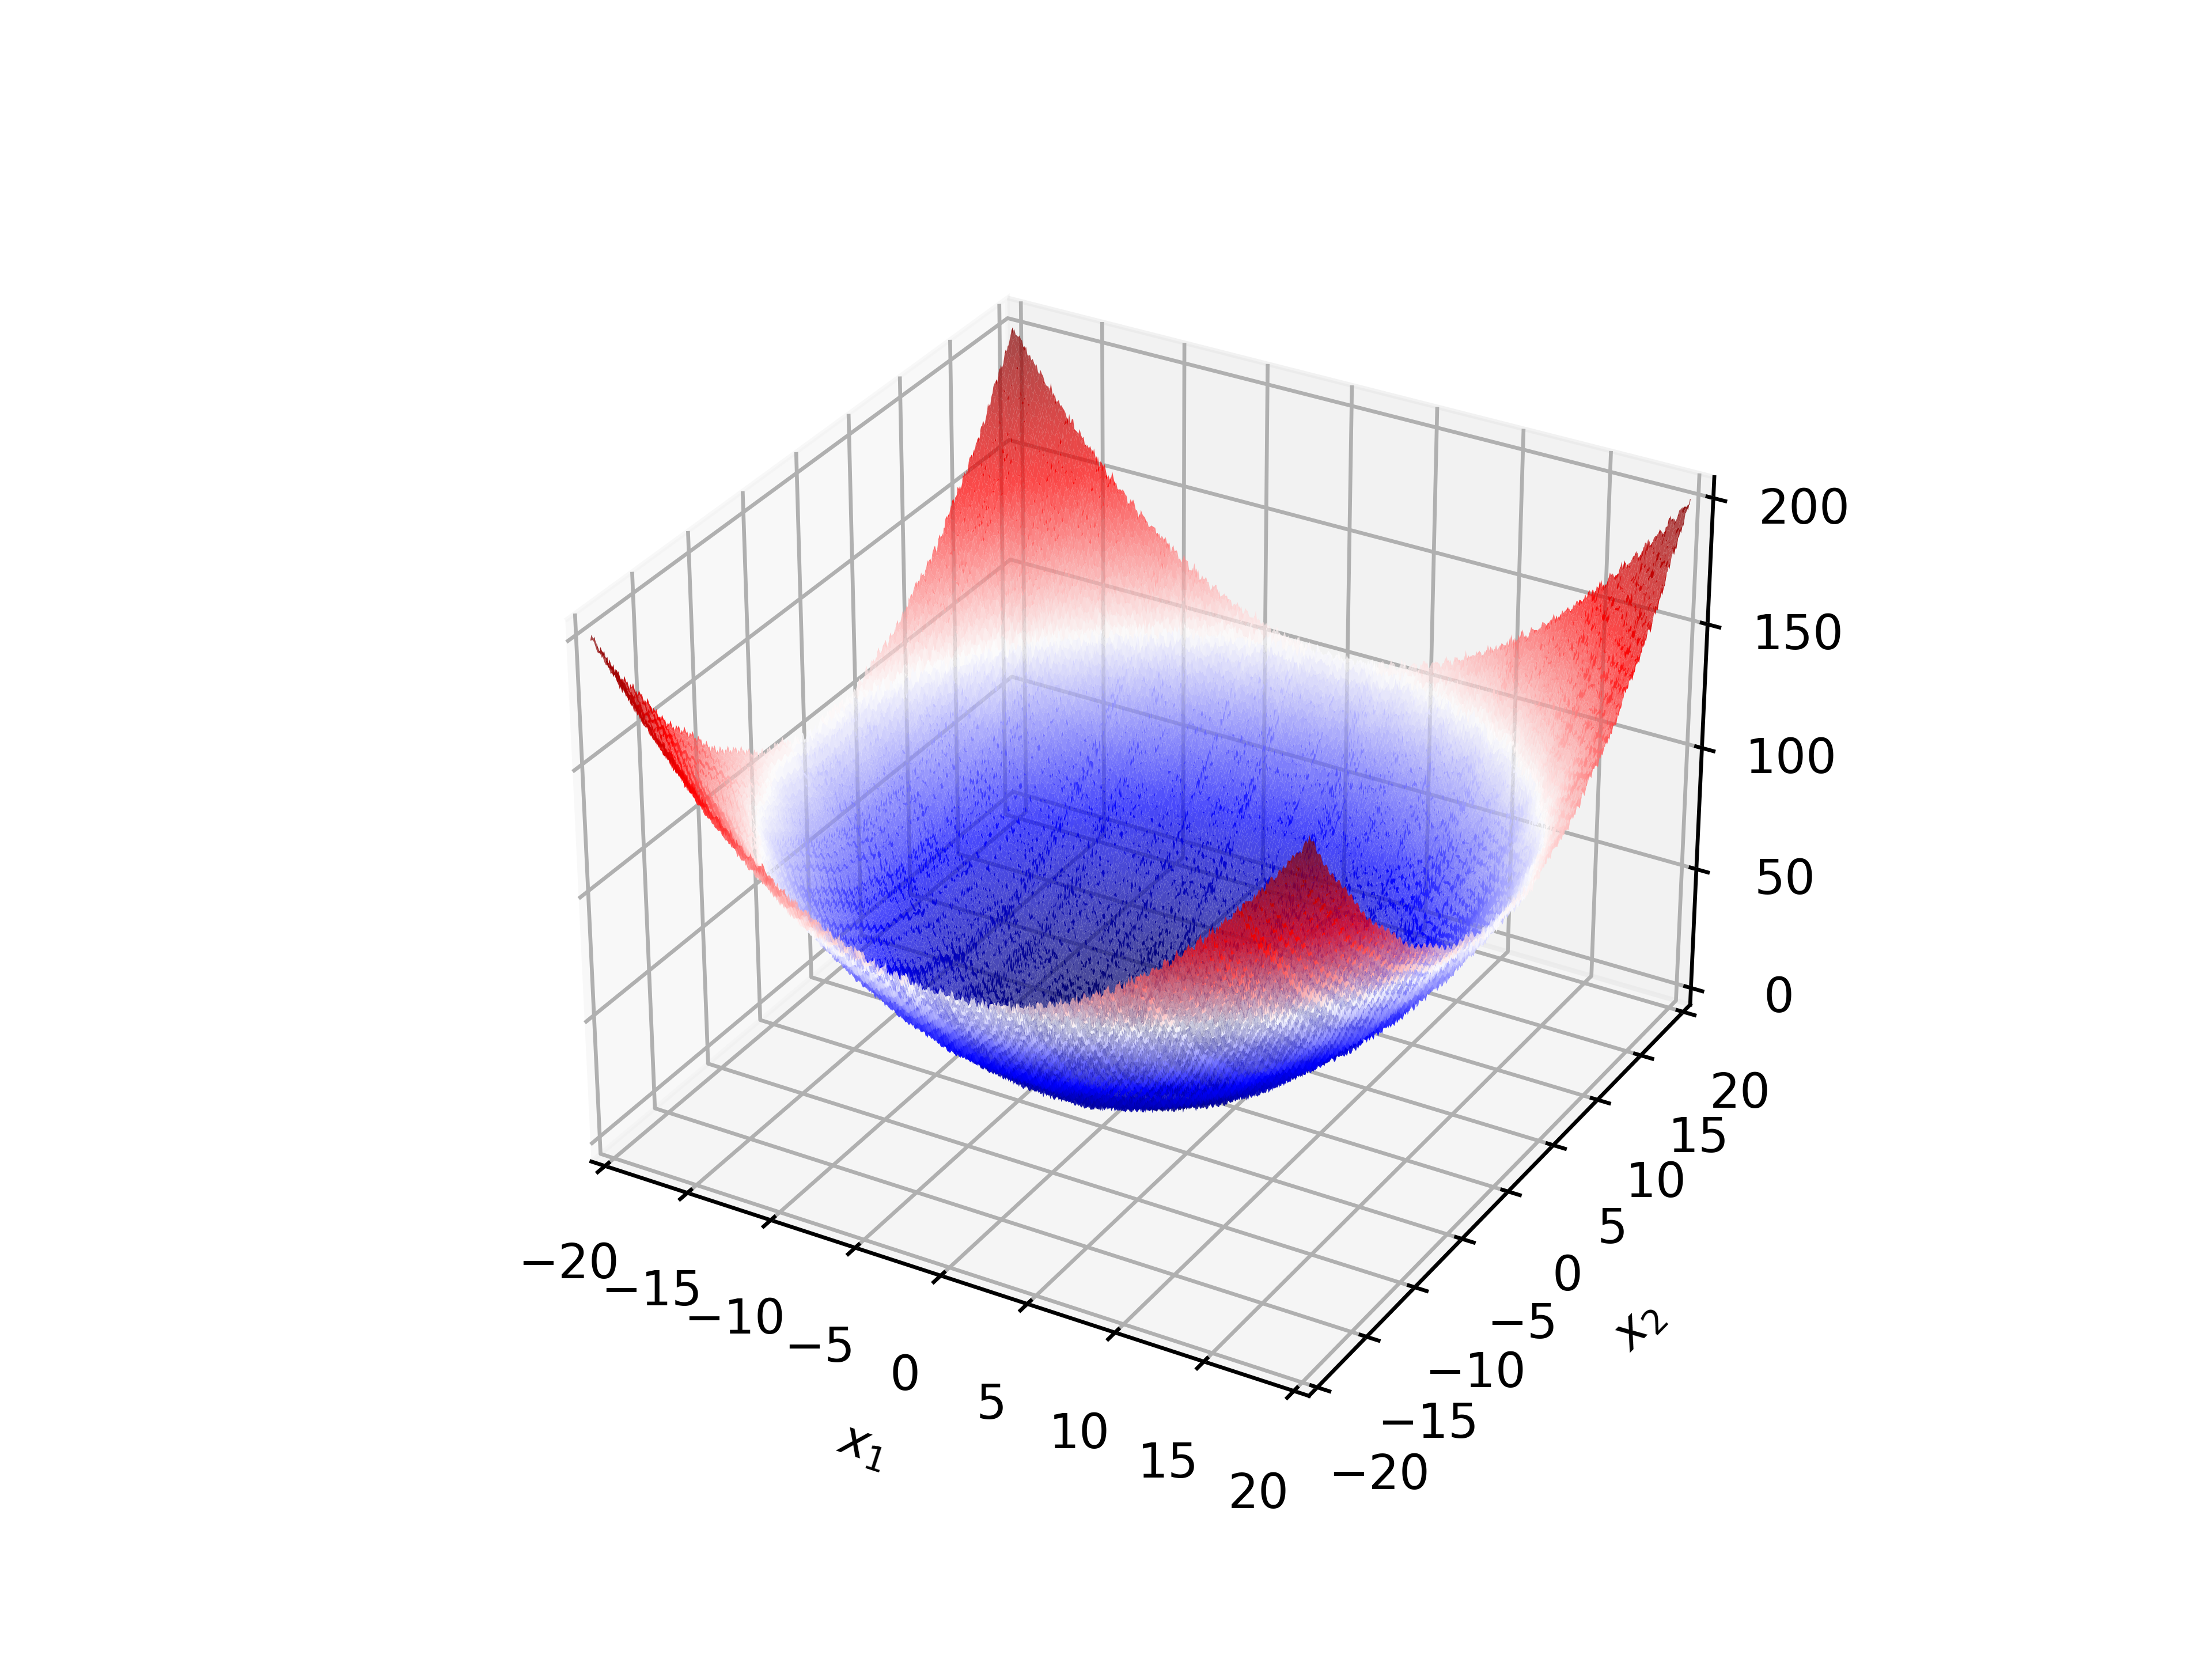
\includegraphics[width=0.525\textwidth]{MathematicalProgrammingf1}&
\hspace*{-0.5cm}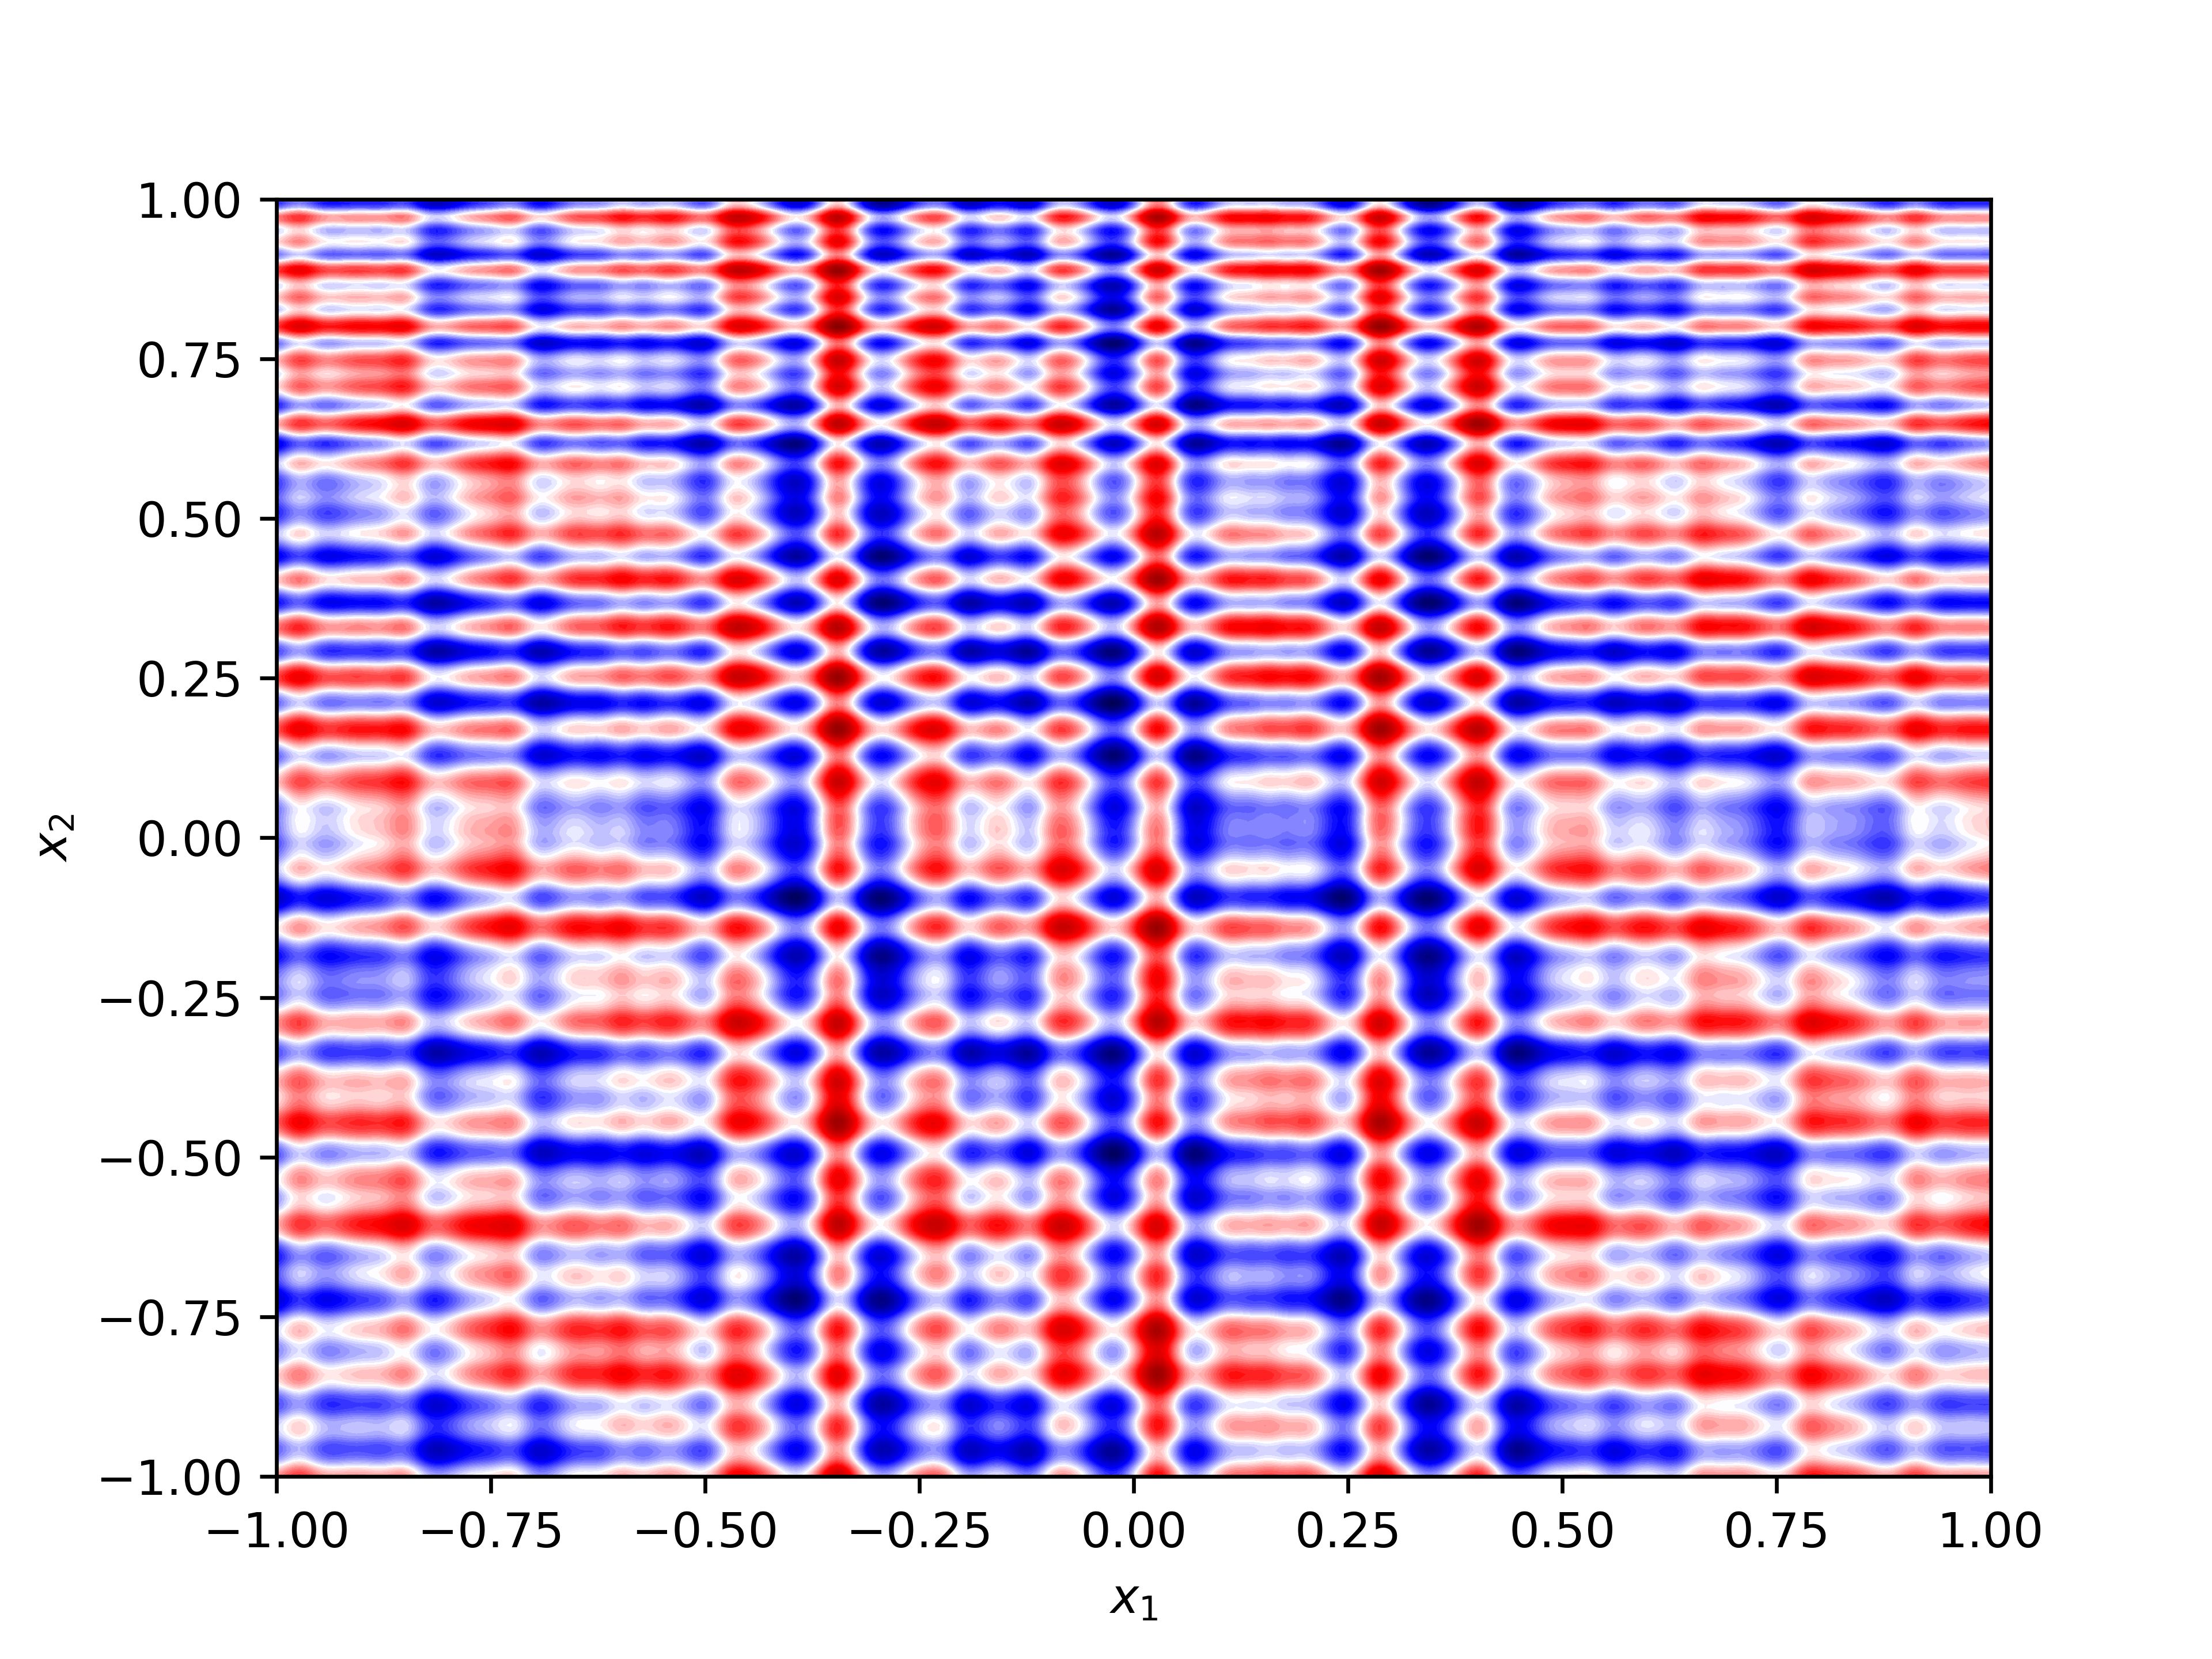
\includegraphics[width=0.525\textwidth]{MathematicalProgrammingf2}\\
(a) & (b)\\
\end{tabular}
\caption{Views of the function~\eqref{eq:SIAM100DigitChallenge}: (a) a surface plot on $[-20,20]^2$ showing the overall paraboloidal shape, and (b) a contour plot on $[-1,1]^2$.}
\label{figure:MathProgf}
\end{center}
\end{figure}

If we evaluate the function at the values of $x_1$ and $x_2$ from $-0.25$ to $0.25$ in steps of $0.01$, we find that the function can be as small as $-3.24$. On the other hand, outside the square $[-1,1]^2$, the function is at least $e^{-1}-1-1-\sin1-1+\frac{1}{4} > -3.23$. Therefore, the global minimum must be inside the square $[-1,1]^2$.

\subsection{Evolutionary Algorithms}

While a grid search can be effective for this particular problem (because the critical points do have a rough lattice structure), it is easy to design a more general search procedure that uses randomness to achieve good coverage of the domain. Several effective algorithms have been derived by abstracting biological processes and theories. Microevolution is a biological theory which describes the dynamics of the gene pool in the members of a species over time. Natural selection and genetic mutation during meiosis are some of the processes that contribute to microevolution. In relation to a NP, for every coordinate $x\in\R^n$, we may associate the {\em fitness value} $f(x)$.

If we begin with a generation of $N_{\rm members}$ random points in a realistic subdomain $D\subset\R^n$, and introduce an additional $N_{\rm members} -1$ points randomly distributed around each of the original $N_{\rm members}$ random points, then we may form a new generation by {\em culling the population} and retaining the $N_{\rm members}$ points-of-best-fit. While we iterate this process, we may use a shrinking scale to define the largest variability of the offspring from their parents.

\begin{algorithm}[Prokaryotic Evolutionary Search]~\\
Inputs: \begin{description} \item[$f(x)$], the objective function;
\item[$D$], the search domain;
\item[$N_{\rm members}$], the number of points in a generation;
\item[$N_{\rm generations}$], the number of generations; and,
\item[$s$], the scaling factor for shrinking the search domain.
\end{description}
Output: an upper bound to the minimum of $f$ in $D$ and its location.
\begin{description}
\item[Step 1:] Initialization:

Let $z$ be the centre of $D$; {\tt parents} = z; and, {\tt fvals = f(z)}.
\item[Step 2:] The main loop:
\begin{verbatim}
for generation = 1:ngenerations
    children = parents
    for p in parents
        append (nmembers-1) random points in D
        centred at p to the children
    end
    fvals = f(children)
    Let parents be the set of nmembers children with lowest fvals
    Shrink D by s
end    
\end{verbatim}
\item[Step 3:] Return:

The smallest value in {\tt fvals} and the corresponding {\tt parent}.
\end{description}
\end{algorithm}

This algorithm may be associated with prokaryotic evolution as the children are strictly descendants from a single parent. If, on the other hand, children may be descendants from two parents, then we obtain a eukaryotic evolutionary search. In the following algorithm, $N_{\rm members}$ children are allowed to be descendants from every pair of parents.

\begin{algorithm}[Eukaryotic Evolutionary Search]~\\
Inputs: \begin{description} \item[$f(x)$], the objective function;
\item[$D$], the search domain;
\item[$N_{\rm members}$], the number of points in a generation; and,
\item[$N_{\rm generations}$], the number of generations.
\end{description}
Output: an upper bound to the minimum of $f$ in $D$ and its location.
\begin{description}
\item[Step 1:] Initialization:

Let {\tt parents} be random points in $D$ and {\tt fvals = f(parents)}.
\item[Step 2:] The main loop:
\begin{verbatim}
for generation = 1:ngenerations
    children = []
    for p in parents, q in parents
        append a random point on the line segment
        in between p and q to the children
    end
    fvals = f(children)
    Let parents be the set of nmembers children with lowest fvals
end    
\end{verbatim}
\item[Step 3:] Return:

The smallest value in {\tt fvals} and the corresponding {\tt parent}.
\end{description}
\end{algorithm}

In Figure~\ref{figure:EvolutionaryAlgorithmError}, an execution of both evolutionary algorithms is depicted for a population with $50$ members, and a scaling factor of $1/2$ for the prokaryotic search. In both (a) and (b), the data represent the discrepancy between the fitness value of every parent in the generation and the global minimum. Clearly, the eukaryotic evolutionary algorithm is able to home in on the global minimum significantly faster than the prokaryotic search. This may be explained as follows: if two parents are equidistant from the global minimum, but on opposite sides (in every coordinate), then we expect a child to appear right over top of the global minimum; on the other hand, no such estimation may be made of prokaryotic evolution.

\begin{figure}[htbp]
\begin{center}
\begin{tabular}{cc}
\hspace*{-0.5cm}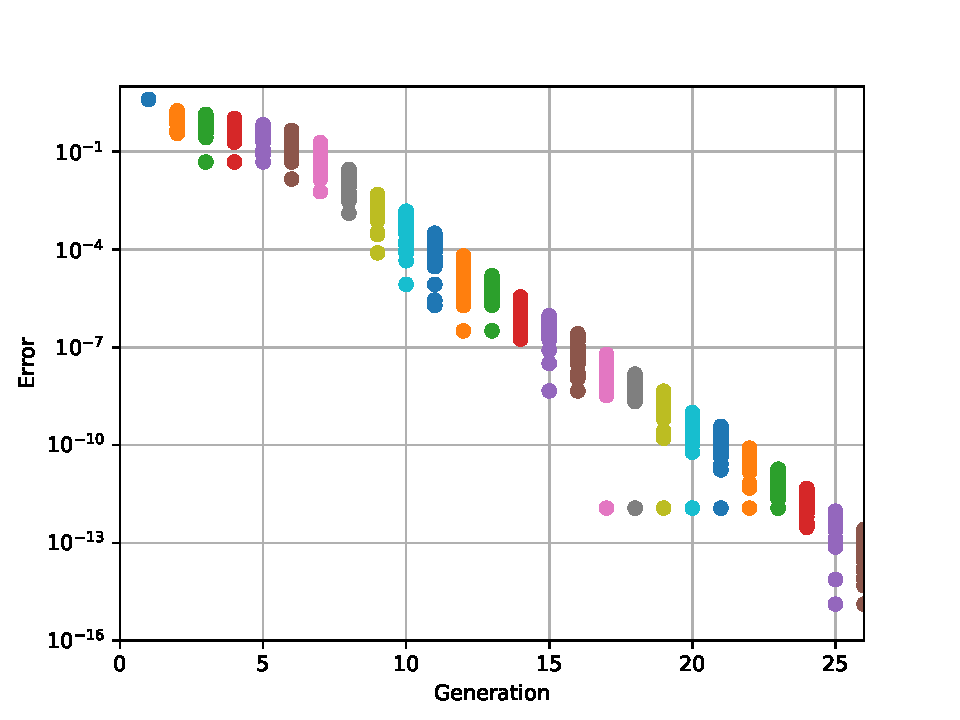
\includegraphics[width=0.525\textwidth]{EvolutionaryAlgorithm1error}&
\hspace*{-0.5cm}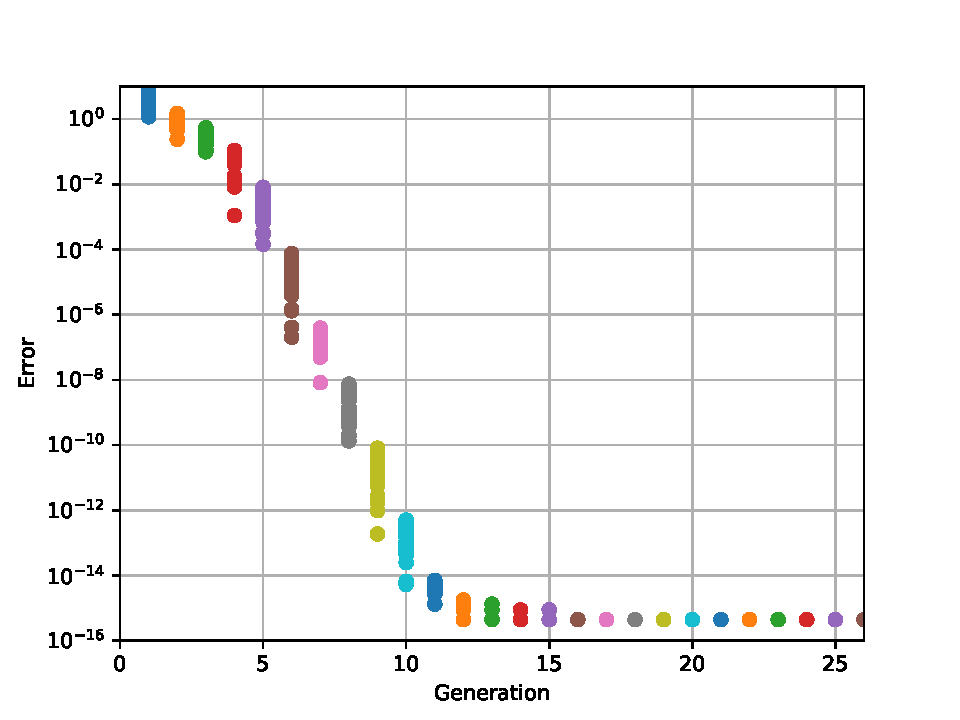
\includegraphics[width=0.525\textwidth]{EvolutionaryAlgorithm2error}\\
(a) & (b)\\
\end{tabular}
\caption{The error of the evolutionary algorithms for the NP~\eqref{eq:SIAM100DigitChallenge} with $50$ members in the population searching through $D=[-1,1]^2$: (a) with prokaryotic search, and (b) with eukaryotic search.}
\label{figure:EvolutionaryAlgorithmError}
\end{center}
\end{figure}

While it is reassuring that the eukaryotic search converges to the global minimum at a faster rate, it is much easier for the algorithm to end up stuck in a local minimizer. Figure~\ref{figure:EvolutionaryAlgorithmProbability} shows the probability of success after $25$ generations of both evolutionary algorithms over $1,000$ iterations. Here, we recognize that the prokaryotic evolutionary search, which supports more random fluctuations throughout the generations, spends more energy ``searching'' through the subdomain $D$ rather than ``settling,'' and is much more likely to succeed with a lower population. This is also reassuring since the earliest living organisms on Earth are thought to be prokaryotes; these organisms had many millions of years to search far and wide for the best (evolutionary) way forward, before eukaryotic search accelerated the process.

\begin{figure}[htbp]
\begin{center}
\begin{tabular}{cc}
\hspace*{-0.5cm}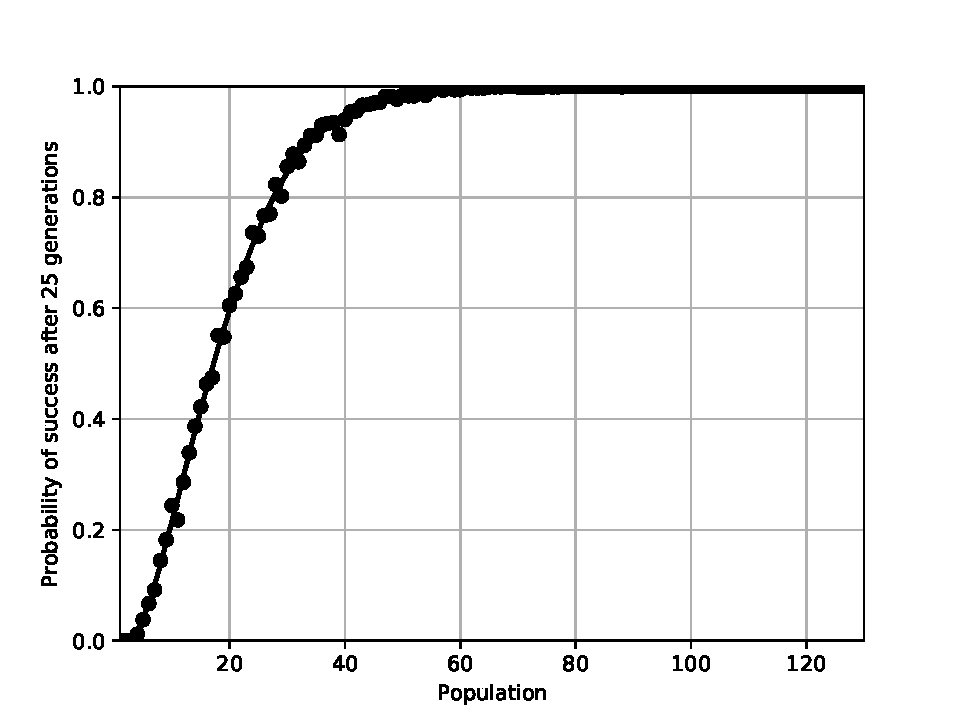
\includegraphics[width=0.525\textwidth]{EvolutionaryAlgorithm1prob}&
\hspace*{-0.5cm}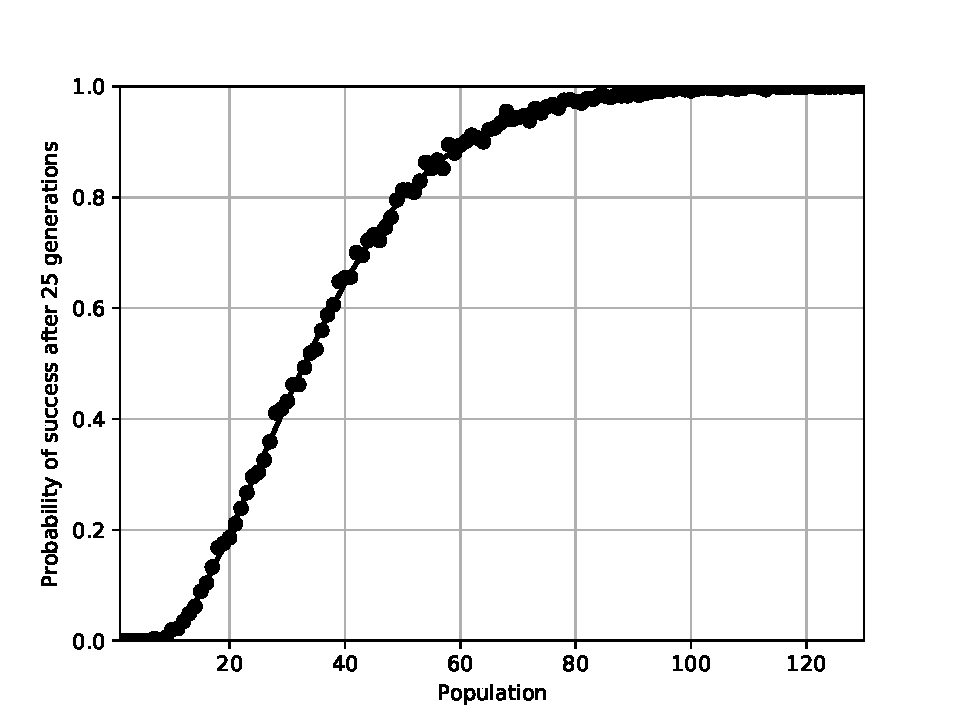
\includegraphics[width=0.525\textwidth]{EvolutionaryAlgorithm2prob}\\
(a) & (b)\\
\end{tabular}
\caption{The probability of success of the evolutionary algorithms over $1,000$ iterations for the NP~\eqref{eq:SIAM100DigitChallenge} searching through $D=[-1,1]^2$: (a) with prokaryotic search, and (b) with eukaryotic search. In both plots, the solid line denotes a degree-$15$ least-squares Chebyshev approximant.}
\label{figure:EvolutionaryAlgorithmProbability}
\end{center}
\end{figure}

Note that both of these algorithms may be adapted to constrained nonlinear programming by rejecting children that do not satisfy the constraints.

\subsection{Quadratic Models}

When we are in striking distance from the global minimizer, we might consider switching to a more efficient algorithm that is able to reproduce extremely high precision results. Recall that a minimizer $x^*$ of a continuously differentiable function $f$ is a critical point:
\[
x^* = \argmin_{x\in\R^n} f(x) \quad \Rightarrow \quad \nabla f(x^*) = 0.
\]
Near a minimizer, we shall approximate a twice continuously differentiable function $f$ by its multivariate Taylor series:
\begin{align*}
f(x+\delta x) & = f(x) + \left[\nabla f(x)\right]^\top \delta x\\
& \quad + \dfrac{1}{2}\delta x^\top \left[\nabla^2 f(x)\right] \delta x + o(\norm{\delta x}^2),\quad {\rm as}\quad \norm{\delta x}\to0.
\end{align*}
To help keep the notation clean, let us introduce $g(x) := \nabla f(x)$ to be the vector of gradients of $f$ and:
\[
H(x) := \nabla^2 f(x) = \begin{bmatrix} \dfrac{\partial^2 f}{\partial x_1^2} & \dfrac{\partial^2 f}{\partial x_1\partial x_2} & \cdots & \dfrac{\partial^2 f}{\partial x_1\partial x_n}\\
\dfrac{\partial^2 f}{\partial x_2\partial x_1} & \dfrac{\partial^2 f}{\partial x_2^2} & \cdots & \dfrac{\partial^2 f}{\partial x_2\partial x_n}\\
\vdots & \vdots & \ddots & \vdots\\
\dfrac{\partial^2 f}{\partial x_n\partial x_1} & \dfrac{\partial^2 f}{\partial x_n\partial x_2} & \cdots & \dfrac{\partial^2 f}{\partial x_n^2}\end{bmatrix},
\]
to be the {\em Hessian}. Then a quadratic approximation to $f$ is:
\[
f(x+\delta x) \approx q(\delta x) = f(x) + g(x)^\top \delta x + \dfrac{1}{2}\delta x^\top H(x) \delta x,
\]
and if we define the vector $\delta x$ by the condition that $\nabla_{\delta x} q(\delta x) = 0$, then we derive Newton's iteration.

\begin{algorithm}[Newton Iteration]~\\
Let $x^{(1)}$ be an initial guess for the global minimizer. For $k\in\N,$
\begin{enumerate}
\item Solve $H(x^{(k)})\delta x^{(k)} = -g(x^{(k)})$, for $\delta x^{(k)}$; and,
\item Set $x^{(k+1)} = x^{(k)} + \delta x^{(k)}$.
\end{enumerate}
\end{algorithm}

The first step in Newton iteration involves the solution of an $n$-by-$n$ system of linear equations. This may be done with a matrix factorization in $\OO(n^3)$ operations\footnote{Quasi-Newton methods are derived by factorizing the matrix $H(x^{(1)})$ once and updating the factorization at every iteration.}. Now that we know how to implement Newton iteration, we may be interested in its convergence properties.

\begin{theorem}
Let $f\in C^2(D)$ and let the Hessian be Lipschitz continuous, i.e. $\abs{H_{i,j}(x) - H_{i,j}(y)} \le K\norm{x-y}$, for some $K>0$, some norm $\norm{\cdot}$, and for $x,y\in D\subset\R^n$. If, for some $k\in\N$, a Newton iterate $x^{(k)}$ is sufficiently close to $x^*\in D$, then Newton's method converges quadratically to $x^*$.
\end{theorem}
\begin{proof}
The Taylor series for each term in $g(x^*)$ is:
\[
0 = g(x^*) = g(x^{(k)}) - H(x^{(k)})e^{(k)} + \OO(\norm{e^{(k)}}^2),
\]
where $e^{(k)} := x^{(k)} - x^*$. Let $x^{(k)}$ be in a neighbourhood of $x^*$ such that $H(x^{(k)})^{-1}$ exists and is bounded above. Such a neighbourhood exists by continuity of $H(x)$. Then, the $k^{\rm th}$ iteration exists, and multiplying through by $H(x^{(k)})^{-1}$ yields:
\[
0 = -\delta x^{(k)} - e^{(k)} + \OO(\norm{e^{(k)}}^2) = -e^{(k+1)} + \OO(\norm{e^{(k)}}^2),
\]
by step 2 of Newton iteration and by definition of $e^{(k+1)}$. Hence by definition of the order notation, there exists a constant $M>0$ such that:
\[
\norm{e^{(k+1)}} \le M\norm{e^{(k)}}^2.
\]
If $x^{(k)}$ is in a neighbourhood for which $\norm{e^{(k)}} < M^{-1}$, then it follows that $\norm{e^{(k+1)}} < \norm{e^{(k)}}$ and by induction, the error contracts and $\displaystyle\lim_{k\to\infty}\norm{e^{(k)}}=0$.
\end{proof}

\section{Linear Programming}

{\em Linear programming} (LP) is a mathematical model for optimizing a linear objective (such as maximum profit or minimum cost) constrained by a list of linear relationships. Linear programming was developed during World War II (independently by the Allies and the Soviet Union) to plan expenditures and returns in order to reduce costs to the army and increase losses to the enemy. It was kept secret until 1947.

The founders of this subject are Leonid Kantorovich, a Russian mathematician who developed LP problems in 1939, George Dantzig, who published the simplex method in 1947, and John von Neumann, who developed the theory of the duality in the same year.

An LP problem in the {\em standard form} is expressed mathematically as:
\mathprog{f(x) := c^\top x}{Ax=b}{x\ge0}{LP:standardform}
where $A\in\R^{m\times n}$ and $m\le n$ (usually $<$). Thus the allowable constraints on the variables are either linear equations or non-negativity bounds. The coefficients $c$ in the linear objective function are often referred to as {\em costs}. An example with four variables ($n=4$) and two equations ($m=2$) is:
\mathprog{x_1 + 2x_2 + 3x_3 + 4x_4}{\begin{array}{rrrrrrrrr} x_1 & + & x_2 & + & x_3 & + & x_4 & = & 1\\
x_1 & & &+ & x_3 & - & 3x_4 & = & \tfrac{1}{2}\end{array}}{x_1\ge0,~x_2\ge0,~x_3\ge0,~x_4\ge0}{LP:example}
More general LP problems can be reduced to standard form without undue difficulty. For example, maximization problems are conveniently re-formulated as $-\hbox{minimize} -f(x)$. Additionally, a general linear inequality $a^\top x \le b$ can be transformed using a slack variable $z$ to the equation $a^\top x + z = b$ and the bound $z\ge 0$. More general bounds $x_i\ge \ell_i$ can be dealt with by a shift of origin, and if no bound exists at all on $x_i$ in the original problem, then the standard form can be reached by introducing non-negative variables $x_i^+$ and $x_i^-$. However, we will concentrate on the solution of problems which are already in the standard form~\eqref{LP:standardform}.

It is important to realize that an LP problem in standard form may have no solution, either because there is no feasible point (the problem is {\em infeasible}), or because $f(x)\to-\infty$ for $x$ in the feasible region (the problem is {\em unbounded}). However, usually there is no difficulty in detecting these situations, and so we will concentrate on the normal case where a solution exists, though it may not be unique.

If~\eqref{LP:standardform} is considered in more detail, it can be seen that if $m=n$, then the equations $Ax=b$ determine a unique solution $x$, and the objective function $c^\top x$ and the bounds $x\ge0$ play no role. In most cases, however, $m<n$ so that the system $Ax=b$ is {\em underdetermined} and $n-m$ degrees of freedom remain. In particular, the system can determine only $m$ variables, given values for the remaining $n-m$ variables. For example, the equations in~\eqref{LP:example-b} can be rearranged as:
\begin{equation}\label{LP:exampleequivalent1}
\begin{array}{rrrrrrr} x_1 & = & \tfrac{1}{2} & - & x_3 & + & 3x_4\\ x_2 & = & \tfrac{1}{2} & & & - & 4x_4\end{array},
\end{equation}
which determines $x_1$ and $x_2$ given values for $x_3$ and $x_4$. Alternatively, the same equations can be rearranged as:
\begin{equation}\label{LP:exampleequivalent2}
\begin{array}{rrrrrrr} x_1 & = & \tfrac{7}{8} & - & \tfrac{3}{4}x_2 & - & x_3\\ x_4 & = & \tfrac{1}{8} & - & \tfrac{1}{4}x_2 &  &\end{array},
\end{equation}
determining $x_1$ and $x_4$ from $x_2$ and $x_3$. It is important to consider what values these remaining $n-m$ variables can take in problems in the standard form. The objective function $c^\top x$ is linear and so contains no curvature which can given rise to a minimizing point. Hence such a point must be created by the conditions $x_i\ge0$ becoming active on the boundary of the feasible region. For example, if~\eqref{LP:exampleequivalent2} is used to eliminate the variables $x_1$ and $x_4$ from the problem~\eqref{LP:example}, then the objective function can be expressed as:
\begin{equation}
c^\top x = x_1 +2x_2 + 3x_3 + 4x_4 = \tfrac{11}{8} + \tfrac{1}{4}x_2 + 2x_3.
\end{equation}
Clearly this function has no minimum value unless the conditions $x_2\ge0$ and $x_3\ge0$ are imposed, in which case the minimum occurs when $x_2=x_3=0$.

To summarize, a solution of an LP problem in standard form always exists at one particular {\em extreme point} or {\em vertex} of the feasible region, with at least $n-m$ variables having {\em zero value}, and the remaining $m$ variables being uniquely determined by the equations $Ax = b$, and taking non-negative values. This result is fundamental to the development of LP methods.

The main difficulty in LP is to find which $n-m$ variables take zero value at the solution and which $m$ variables are not. The first algorithm to solve LP problems is the {\em simplex method}, which tries different sets of possibilities in a systematic way.

\subsection{The Simplex Method}

The simplex method for solving an LP problem in standard form generates a sequence of feasible points $x^{(1)}, x^{(2)},\ldots$ which terminates at a solution. Since there exists a vertex at which the solution occurs, each iterate $x^{(k)}$ is also a vertex. Thus $m$ variables have a non-negative value (usually positive) at $x^{(k)}$ and are referred to as {\em basic variables}, and the remaining $n-m$ variables have zero value and are referred to as {\em nonbasic variables}. In each iteration, the simplex method swaps a basic and nonbasic variable in order to decrease the objective function. The superscript $(k)$ is often omitted for clarity.

In the simplex method, we start by partitioning $A = [A_B | A_N]$ where $A_B$ is non-singular. Partitioning $x^\top = (x_B^\top, x_N^\top)$ conformably and $c^\top = (c_B^\top,c_N^\top)$, then we may write the LP problem~\eqref{LP:standardform} in {\em tableau form}:
\[
\left[\begin{array}{c|c} c^\top & 0\\\hline A & b\end{array}\right] = \left[\begin{array}{cc|c} c_B^\top & c_N^\top & 0\\\hline A_B & A_N & b\end{array}\right].
\]
\begin{example}
The LP problem~\eqref{LP:example} can be reformulated as:
\[
\left[\begin{array}{cccc|c} 1 & 2 & 3 & 4 & 0\\\hline 1 & 1 & 1 & 1 & 1\\ 1 & 0 & 1 & -3 & \tfrac{1}{2}\end{array}\right].
\]
The $2$-by-$2$ sub-block in the lower left is non-singular, $\begin{vmatrix} 1 & 1\\ 1 & 0\end{vmatrix} = -1$, and thus we start by identifying $x_1$ and $x_2$ as the basic variables.
\end{example}
Then, by performing {\em row operations} on the tableau (adding or subtracting multiples of one row from another, or by scaling any row), it is possible to reduce the tableau to the form:
\[
\left[\begin{array}{cc|c} c_B^\top & c_N^\top & 0\\\hline A_B & A_N & b\end{array}\right] \rightarrow \left[\begin{array}{cc|c} 0^\top & \hat{c}_N^\top & -\hat{f}\\\hline I & \hat{A}_N & \hat{b}\end{array}\right],
\]
where $\hat{A}_N = A_B^{-1}A_N$, which represents the {\em reduced form} of the LP problem.
\begin{example}
Performing row operations on the LP problem~\eqref{LP:example}:
\begin{align*}
\begin{array}{c} r_1\leftarrow r_1-r_2\\r_3\leftarrow r_2-r_3\end{array} \Rightarrow \left[\begin{array}{cccc|c} 0 & 1 & 2 & 3 & -1\\\hline 1 & 1 & 1 & 1 & 1\\ 0 & 1 & 0 & 4 & \tfrac{1}{2}\end{array}\right],\\
\begin{array}{c} r_1\leftarrow r_1-r_3\\r_2\leftarrow r_2-r_3\end{array} \Rightarrow \left[\begin{array}{cccc|c} 0 & 0 & 2 & -1 & -\tfrac{3}{2}\\\hline 1 & 0 & 1 & -3 & \tfrac{1}{2}\\ 0 & 1 & 0 & 4 & \tfrac{1}{2}\end{array}\right].
\end{align*}
At this stage, the reduced LP problem is equivalent to:
\mathprog{\tfrac{3}{2} + 2x_3 - x_4}{\begin{array}{rrrrrrrrr} x_1 & & & + & x_3 & - & 3x_4 & = & \tfrac{1}{2}\\
& & x_2 & & & + & 4x_4 & = & \tfrac{1}{2}\end{array}}{x_1\ge0,~x_2\ge0,~x_3\ge0,~x_4\ge0}{LP:examplereduced}
While originally the variables $x_3$ and $x_4$ are the nonbasic variables, and thereby $0$, generally they must be non-negative. Therefore, since the coefficient of $x_4$ is $-1$, a positive perturbation of $x_4$ (less than $1/8$ otherwise $x_2$ would fail its non-negativity constraint!) will decrease the objective.
\end{example}
The next step is to analyze the reduced costs $\hat{c}_N$. If the current vertex is optimal, then the reduced costs satisfy the test:
\begin{equation}\label{eq:LPtest}
\hat{c}_N \ge 0.
\end{equation}
If not, then we permute the nonbasic variable associated with the most negative cost:
\[
j = \argmin_{1\le i \le n-m} [\hat{c}_N]_i,
\]
for the basic variable which is forced to violate its non-negativity constraint first. Row operations are again performed to recover the reduced form of the LP problem. The simplex algorithm terminates when all the reduced costs in the final iteration satisfy the test~\eqref{eq:LPtest}.
\begin{example}
In the LP problem~\eqref{LP:example}, $-1$ is the lowest element in the vector of reduced costs. Therefore, we introduce row operations to make a basis vector to then permute with the basic variable $x_2$:
\begin{align*}
\begin{array}{c} r_3\leftarrow \tfrac{1}{4}r_3\\\end{array} \Rightarrow \left[\begin{array}{cccc|c} 0 & 0 & 2 & -1 & -\tfrac{3}{2}\\\hline 1 & 0 & 1 & -3 & \tfrac{1}{2}\\ 0 & \tfrac{1}{4} & 0 & 1 & \tfrac{1}{8}\end{array}\right],\\
\begin{array}{c} r_1\leftarrow r_1+r_3\\r_2\leftarrow r_2+3r_3\end{array} \Rightarrow \left[\begin{array}{cccc|c} 0 & \tfrac{1}{4} & 2 & 0 & -\tfrac{11}{8}\\\hline 1 & \tfrac{3}{4} & 1 & 0 & \tfrac{7}{8}\\ 0 & \tfrac{1}{4} & 0 & 1 & \tfrac{1}{8}\end{array}\right],\\
\begin{array}{c} c_2\leftrightarrow c_4\\\end{array} \Rightarrow \left[\begin{array}{cccc|c} 0 & 0 & 2 & \tfrac{1}{4} & -\tfrac{11}{8}\\\hline 1 & 0 & 1 & \tfrac{3}{4} & \tfrac{7}{8}\\ 0 & 1 & 0 & \tfrac{1}{4} & \tfrac{1}{8}\end{array}\right].
\end{align*}
After one iteration, the reduced costs are all positive, satisfying the test~\eqref{eq:LPtest}, and therefore we know that the nonbasic variables are exactly $0$. Therefore, the solution to the LP problem~\eqref{LP:example} is $\tfrac{11}{8}$, satisfied by:
\[
x_1 = \tfrac{7}{8},~x_2 = 0,~x_3=0,~x_4 = \tfrac{1}{8}.
\]
\end{example}

\begin{remark}
If more than one iteration of the simplex method is required, it may be difficult for you to keep track of the variables after multiple column permutations. Therefore, it is sufficient to ensure that columns of the identity matrix are present {\em somewhere} in the reduced form at each iteration. The simplex algorithm still terminates when all the reduced costs are positive.
\end{remark}

\begin{example}
\mathprog{\begin{array}{rrrrrrrrr} x_1 & + & 3x_2 & + & x_3 & + & 2x_4 & + & x_5\end{array}}{\begin{array}{rrrrrrrrrrr} x_1 & & & + & 2x_3 & & & + & 4x_5 & = & 3\\
& & 2x_2 & & & + & 3x_4 & & & = & 1\\ x_1 & + & x_2 & + & x_3 & & & & & = & 2\\\end{array}}{x_1\ge0,~x_2\ge0,~x_3\ge0,~x_4\ge0,~x_5\ge0}{LP:example2}
In tableau form, the LP problem is:
\[
\left[\begin{array}{ccccc|c} 1 & 3 & 1 & 2 & 1 & 0\\\hline 1 & 0 & 2 & 0 & 4 & 3\\ 0 & 2 & 0 & 3 & 0 & 1\\ 1 & 1 & 1 & 0 & 0 & 2\end{array}\right].
\]
We perform row operations to obtain a reduced form. Note that the lower left $3$-by-$3$ sub-block is non-singular.
\begin{align*}
\begin{array}{c} ~\\r_3 \leftarrow \tfrac{1}{2}r_3\end{array} \Rightarrow \left[\begin{array}{ccccc|c} 1 & 3 & 1 & 2 & 1 & 0\\\hline 1 & 0 & 2 & 0 & 4 & 3\\ 0 & 1 & 0 & \tfrac{3}{2} & 0 & \tfrac{1}{2}\\ 1 & 1 & 1 & 0 & 0 & 2\end{array}\right]\\
\begin{array}{c} r_1 \leftarrow r_1-r_2\\~\\~\\r_4\leftarrow r_2+r_3-r_4\end{array} \Rightarrow \left[\begin{array}{ccccc|c} 0 & 3 & -1 & 2 & -3 & -3\\\hline 1 & 0 & 2 & 0 & 4 & 3\\ 0 & 1 & 0 & \tfrac{3}{2} & 0 & \tfrac{1}{2}\\ 0 & 0 & 1 & \tfrac{3}{2} & 4 & \tfrac{3}{2}\end{array}\right]\\
\begin{array}{c} r_1 \leftarrow r_1-3r_3+r_4\\r_2\leftarrow r_2-2r_4\\~\\~\end{array} \Rightarrow \left[\begin{array}{ccccc|c} 0 & 0 & 0 & \circled{$-{\rm 1}$} & 1 & -3\\\hline 1 & 0 & 0 & -3 & -4 & 0\\ 0 & 1 & 0 & \fbox{$\tfrac{3}{2}$} & 0 & \tfrac{1}{2}\\ 0 & 0 & 1 & \tfrac{3}{2} & 4 & \tfrac{3}{2}\end{array}\right].
\end{align*}
Now in reduced form, we find that the first reduced cost $[\hat{c}_B]_1<0$, circled, so we will be permuting with the nonbasic variable $x_4$. The second row in the tableau shows that $x_1 -3x_4 - 4x_5=0$. Therefore, increasing $x_4$ will not violate the non-negativity of $x_1$. The third row in the tableau shows that $x_2+\tfrac{3}{2}x_4 = \tfrac{1}{2}$, implying that $x_2$ violates the non-negativity constraint when $x_4\ge\tfrac{1}{3}$. On the other hand, the fourth row in the tableau shows that $x_3+\tfrac{3}{2}x_4+4x_5 = \tfrac{3}{2}$, implying that $x_3$ violates the non-negativity constraint when $x_4\ge1$. Thus, by increasing the nonbasic variable $x_4$, the basic variable $x_2$ will violate the non-negativity constraint before $x_3$. Therefore, the pivot is boxed.
\begin{align*}
\begin{array}{c} ~\\r_3 \leftarrow \tfrac{2}{3}r_3\end{array} \Rightarrow \left[\begin{array}{ccccc|c} 0 & 0 & 0 & -1 & 1 & -3\\\hline 1 & 0 & 0 & -3 & -4 & 0\\ 0 & \tfrac{2}{3} & 0 & 1 & 0 & \tfrac{1}{3}\\ 0 & 0 & 1 & \tfrac{3}{2} & 4 & \tfrac{3}{2}\end{array}\right],\\
\begin{array}{c} r_1\leftarrow r_1+r_3\\r_2\leftarrow r_2 + 3r_3\\~\\r_4\leftarrow r_4-\tfrac{3}{2}r_3\end{array} \Rightarrow \left[\begin{array}{ccccc|c} 0 & \tfrac{2}{3} & 0 & 0 & 1 & -\tfrac{8}{3}\\\hline 1 & 2 & 0 & 0 & -4 & 1\\ 0 & \tfrac{2}{3} & 0 & 1 & 0 & \tfrac{1}{3}\\ 0 & -1 & 1 & 0 & 4 & 1\end{array}\right].
\end{align*}
We have returned the LP problem again to reduced form, but this time the reduced costs are all positive. The minimum of $\tfrac{8}{3}$ is attained at $x = (1,0,1,\tfrac{1}{3},0)^\top$.
\end{example}

It became apparent that the tableau form is inefficient in that it updates the entire tableau $\hat{A}_N$ at each iteration. In fact, all the operations in the simplex method can be carried out with an explicit knowledge of $A_B^{-1}$. Since $A_B^{-1}$ is often smaller than $\hat{A}_N$, the resulting method, known as the {\em revised simplex method}, is usually more efficient. The effect of a basis change is to replace the column $a_p$ by $a_q$ in $A_B^{(k)}$, which can be written as the rank-one change:
\[
A_B^{(k+1)} = A_B^{(k)} + (a_q-a_p)e_p^\top.
\]
By using the Sherman--Morrison formula:
\[
\left(A+uv^\top\right)^{-1} = A^{-1} - \dfrac{A^{-1}uv^\top A^{-1}}{1+v^\top A^{-1}u},
\]
we can update the inverse of $A_B^{(k+1)}$ directly.

For LP problems over hundreds of variables, the Sherman--Morrison formula leads to instabilities due to amplification of rounding errors. Instead, well-conditioned matrix factorizations, such as the $QR$ factorization are employed to ensure stability. The rank-one update can similarly be effected in the $Q$ and $R$ factors. For LP problems over tens of thousands of variables, the sparsity of the matrix $A$ is captured, and a pivoting strategy is used to preserve as much of the original sparsity in the {\em factors} as possible. This is an area of active research.

\section{Problems}

\begin{enumerate}

\item What and where is the global minimum of the function:
\begin{align*}
f(x) & = e^{\sin(50x_1)} + \sin(60e^{x_2})\sin(60x_3) + \sin(70\sin(x_1))\cos(10x_3)\\
& \quad + \sin(\sin(80x_2)) - \sin(10(x_1+x_3)) + (x_1^2+x_2^2+x_3^2)/4~?
\end{align*}

\item Solve the linear program:
\mathprog{\begin{array}{rrrrrrrrrrr} 3x_1 & + & 5x_2 & + & 4x_3 & + & 2x_4 & + & x_5\end{array}}{\begin{array}{rrrrrrrrrrr} x_1 & & & - & 2x_3 & & & + & 4x_5 & = & 1\\
-x_1 & + & 2x_2 & + & 5x_3 & + & 3x_4 & & & = & 2\\ x_1 & & & + & x_3 & + & 2x_4 & & & = & 1\\\end{array}}{x_1\ge0,~x_2\ge0,~x_3\ge0,~x_4\ge0,~x_5\ge0}{LP:problem}

\end{enumerate}

\bibliography{/Users/Mikael/Bibliography/Mik}

\end{document}